\chapter{Atomic Combinations}
\label{chap:bonding}

When you look at the matter, or physical substances, around you, you will realise that atoms seldom exist on their own. More often, the things around us are made up of different atoms that have been joined together. This is called \textbf{chemical bonding}. Chemical bonding is one of the most important processes in chemistry because it allows all sorts of different molecules and combinations of atoms to form, which then make up the objects in the complex world around us. There are, however, some atoms that \textit{do} exist on their own, and which do not bond with others. The \textbf{noble gases} in Group 8 of the Periodic Table behave in this way. They include elements like neon (Ne), helium (He) and argon (Ar). The important question then is, why do some atoms bond but others do not?


% CHILD SECTION START 

\section{Why do atoms bond?}
\label{sec:bonding:why do atoms bond}

As we begin this section, it's important to remember that what we will go on to discuss is a \textit{model} of bonding, that is based on a particular \textit{model} of the atom. You will remember from the discussion on atoms 
%section \ref{sec:atom:models} 
that a model is a \textit{representation} of what is happening in reality. In the model of the atom that you are familiar with, the atom is made up of a central nucleus, surrounded by electrons that are arranged in fixed energy levels (sometimes called \textit{shells}). Within each energy level, electrons move in \textit{orbitals} of different shapes. The electrons in the outermost energy level of an atom are called the \textbf{valence electrons}. This model of the atom is useful in trying to understand how different types of bonding take place between atoms.\\

You will remember from these earlier discussions of electrons and energy levels in the atom, that electrons always try to occupy the \textit{lowest} possible energy level. In the same way, an atom also prefers to exist in the lowest possible energy state so that it is most \textit{stable}. An atom is most stable when all its valence electron orbitals are \textit{full}. In other words, the outer energy level of the atom contains the maximum number of electrons that it can. A stable atom is also an \textit{unreactive} one, and is unlikely to bond with other atoms. This explains why the noble gases are unreactive and why they exist as atoms, rather than as molecules. Look for example at the electron configuration of neon (1s$^{2}$ 2s$^{2}$ 2p$^{6}$). Neon has eight valence electrons in its valence energy shell. This is the maximum that it can hold and so neon is very stable and unreactive, and will not form new bonds. Other atoms, whose valence energy levels are not full, are more likely to bond in order to become more stable. We are going to look a bit more closely at some of the energy changes that take place when atoms bond. 


% CHILD SECTION END 



% CHILD SECTION START 

\section{Energy and bonding}

Let's start by imagining that there are two hydrogen atoms approaching one another. As they move closer together, there are three forces that act on the atoms at the same time. These forces are shown in figure \ref{fig:bondingforces} and are described below:\\

\begin{figure}[!h]
\begin{center}
\begin{pspicture}(-4,-1.5)(4,2)
%\psgrid[gridcolor=lightgray]

\def\bondingforces{\psellipse(-2,0)(1.2,1.2)
\psellipse(2,0)(1.2,1.2)
\psellipse(-2,0)(0.4,0.4)
\psellipse(2,0)(0.4,0.4)
\rput(-2,0){\textbf{+}}
\rput(2,0){\textbf{+}}
\psline(-2.1,0.9)(-1.9,0.9)
\psline(2.1,0.9)(1.9,0.9)
\psline[arrows=<->](-1.7,0.9)(1.7,0.9)
\psline[arrows=<->](-1.7,0.8)(1.5,0.1)
\psline[arrows=<->](-1.5,0)(1.5,0)
\rput(0,1.1){(1)}
\rput(0,0.6){(2)}
\rput(0,0.2){(3)}}
\rput(0,0){\psset{unit=1.5}\bondingforces}
\end{pspicture}
\end{center}
\caption{Forces acting on two approaching atoms: (1) repulsion between electrons, (2) attraction between protons and electrons and (3) repulsion between protons.}
\label{fig:bondingforces}
\end{figure}

\begin{enumerate}
\item{\textbf{repulsive force} between the electrons of the atoms, since like charges repel}
\item{\textbf{attractive force} between the nucleus of one atom and the electrons of another}
\item{\textbf{repulsive force} between the two positively-charged nuclei} 
\end{enumerate}

Now look at figure \ref{fig:bonding:energy} to understand the energy changes that take place when the two atoms move towards each other. \\

\begin{figure}[!h]
\begin{center}
\scalebox{1.2}{
\begin{pspicture}(-4,-4)(6,4)
%\psgrid

\psaxes[ticks=none,labels=none](-4,0)(-4,-3.5)(6,3.5)
\psplot{-3.6}{6}{0.15 x 10 add mul -12 exp 0.15 x 10 add mul -6 exp sub 
10 mul}

\rput{90}(-5,0){Energy}
\psline{->}(-4.7,-2.5)(-4.7,2.5)
\uput[l](-4,3){+}
\uput[l](-4,0){0}
\uput[l](-4,-3){-}

\rput[u](3.5,1){Distance between atomic nuclei}
\psline{->}(1,0.6)(6,0.6)
\uput[u](6,0){A}

\pnode(-2.5,0){qTop}
\pnode(-2.5,-2.5){qBottom}
\pnode(-4,0.4){pLeft}
\pnode(-2.5,0.4){pRight}

\ncline{<->}{qTop}{qBottom}
\Aput{Q}
\ncline{<->}{pLeft}{pRight}
\Aput{P}

\uput[d](-2.5,-2.5){X}

\end{pspicture}
}
\caption{Graph showing the change in energy that takes place as atoms move closer together}
\label{fig:bonding:energy}
\end{center}
\end{figure}

In the example of the two hydrogen atoms, where the resultant force between them is attraction, the energy of the system is zero when the atoms are far apart (point A), because there is no interaction between the atoms. When the atoms move closer together, attractive forces dominate and the atoms are pulled towards each other. As this happens, the \textit{potential energy} of the system decreases because energy would now need to be \textit{supplied} to the system in order to move the atoms apart. However, as the atoms continue to move closer together (i.e. \textit{left} along the horizontal axis of the graph), repulsive forces start to dominate and this causes the potential energy of the system to rise again. At some point, the attractive and repulsive effects are balanced, and the energy of the system is at its minimum (point X). It is at this point, when the energy is at a minimum, that bonding takes place.\\

The distance marked 'P' is the \textbf{bond length}, i.e. the distance between the nuclei of the atoms when they bond. 'Q' represents the \textbf{bond energy} i.e. the amount of energy that must be added to the system to break the bonds that have formed. \textbf{Bond strength} means how strongly one atom attracts and is held to another. The strength of a bond is related to the bond length, the size of the bonded atoms and the number of bonds between the atoms. In general, the shorter the bond length, the stronger the bond between the atoms, and the smaller the atoms involved, the stronger the bond. The greater the number of bonds between the atoms, the greater the bond strength.
Phet simulation on atomic interactions:SIYAVULA-SIMULATION:http://cnx.org/content/m38892/latest/#id63458

% CHILD SECTION END 



% CHILD SECTION START 

\section{What happens when atoms bond?}
\label{sec:bonding:what happens}

A \textbf{chemical bond} is formed when atoms are held together by attractive forces. This attraction occurs when electrons are \textit{shared} between atoms, or when electrons are \textit{exchanged} between the atoms that are involved in the bond. The sharing or exchange of electrons takes place so that the outer energy levels of the atoms involved are filled and the atoms are more stable. If an electron is \textbf{shared}, it means that it will spend its time moving in the electron orbitals around \textit{both} atoms. If an electron is \textbf{exchanged} it means that it is transferred from one atom to another, in other words one atom \textit{gains} an electron while the other \textit{loses} an electron.

\Definition{Chemical bond}{A chemical bond is the physical process that causes atoms and molecules to be attracted to each other, and held together in more stable chemical compounds.}

The type of bond that is formed depends on the elements that are involved. In this section, we will be looking at three types of chemical bonding: \textbf{covalent}, \textbf{ionic} and \textbf{metallic bonding}.

You need to remember that it is the \textit{valence electrons} that are involved in bonding and that atoms will try to fill their outer energy levels so that they are more stable.


% CHILD SECTION END 



% CHILD SECTION START 

\section{Covalent Bonding}
\label{subsec:bonding:covalent}

\subsection{The nature of the covalent bond}

Covalent bonding occurs between the atoms of \textbf{non-metals}. The outermost orbitals of the atoms overlap so that unpaired electrons in each of the bonding atoms can be shared. By overlapping orbitals, the outer energy shells of all the bonding atoms are filled. The shared electrons move in the orbitals around \textit{both} atoms. As they move, there is an attraction between these negatively charged electrons and the positively charged nuclei, and this force holds the atoms together in a covalent bond. 

\Definition{Covalent bond}{Covalent bonding is a form of chemical bonding where pairs of electrons are shared between atoms.}

Below are a few examples. Remember that it is only the \textit{valence electrons} that are involved in bonding, and so when diagrams are drawn to show what is happening during bonding, it is only these electrons that are shown. Circles and crosses represent electrons in different atoms.\\
The following simulation allows you to build some simple covalent molecules.
Phet simulation on covalent molecules:SIYAVULA-SIMULATION:http://cnx.org/content/m38895/latest/#id6348
\begin{wex}{Covalent bonding}{How do hydrogen and chlorine atoms bond covalently in a molecule of hydrogen chloride?}{\westep{Determine the electron configuration of each of the bonding atoms.}
A chlorine atom has 17 electrons, and an electron configuration of 1s$^{2}$ 2s$^{2}$ 2p$^{6}$ 3s$^{2}$ 3p$^{5}$. A hydrogen atom has only 1 electron, and an electron configuration of 1s$^{1}$.
\westep{Determine the number of valence electrons for each atom, and how many of the electrons are paired or unpaired.}
Chlorine has 7 valence electrons. One of these electrons is unpaired. Hydrogen has 1 valence electron and it is unpaired.
\westep{Look to see how the electrons can be shared between the atoms so that the outermost energy levels of both atoms are full.}
The hydrogen atom needs one more electron to complete its valence shell. The chlorine atom also needs one more electron to complete its shell. Therefore \textit{one pair of electrons} must be shared between the two atoms. In other words, one electron from the chlorine atom will spend some of its time orbiting the hydrogen atom so that hydrogen's valence shell is full. The hydrogen electron will spend some of its time orbiting the chlorine atom so that chlorine's valence shell is also full. A molecule of hydrogen chloride is formed (figure \ref{fig:bonding:hydrogen chloride}). Notice the shared electron pair in the overlapping orbitals.
\begin{figure}[H]
\begin{center}
\scalebox{0.7}{
\begin{pspicture}(-7,-4.5)(7,1.5)
%\psgrid
\rput(-3.5,-1.8){\textbf{+}}
% Lower left
\uput[u](-5,-2){
\pscircle(0,0){1}
\qdisk(0.83,0.45){0.2}
\pscircle(3.5,0){1.5}
\uput{0}[u](0,-.2){\scalebox{2}{H}}

\rput(1.25,0){ 
\uput[d](0.83,-0.1){ \scalebox{2}{x}}
\uput{0.01}[l](2.25,1.5){ \scalebox{2}{x}}
\uput{0.01}[r](2.25,1.5){ \scalebox{2}{x}}
\uput[u](3.65,0){ \scalebox{2}{x}}
\uput[d](3.65,0){ \scalebox{2}{x}}
\uput{0.01}[l](2.25,-1.45){ \scalebox{2}{x}}
\uput{0.01}[r](2.25,-1.45){ \scalebox{2}{x}} 
\uput{0}[u](2.25,-.2){\scalebox{2}{Cl}}
}
}

% \psline{->}(0.5,2)(1.5,2)
\psline{->}(0.65,-2)(1.65,-2)

% Lower right
\uput[u](3,-2){
\pscircle(0,0){1}
\pscircle(2.25,0){1.5}
\qdisk(0.83,0.45){0.2}
\uput{0}[u](0,-.2){\scalebox{2}{H}}

\uput[d](0.83,-0.1){ \scalebox{2}{x}}
\uput{0.01}[l](2.25,1.5){ \scalebox{2}{x}}
\uput{0.01}[r](2.25,1.5){ \scalebox{2}{x}}
\uput[u](3.65,0){ \scalebox{2}{x}}
\uput[d](3.65,0){ \scalebox{2}{x}}
\uput{0.01}[l](2.25,-1.45){ \scalebox{2}{x}}
\uput{0.01}[r](2.25,-1.45){ \scalebox{2}{x}} 
\uput{0}[u](2.25,-.2){\scalebox{2}{Cl}}
}
\psline(-4,-1.5)(-3.5,-4)
\psline(-3,-2.5)(-3.5,-4)
\rput(-3.5,-4.4){\Large{unpaired electrons}}
\psline[arrows=<-](-1.5,0)(0,1)
\rput(2,1.5){\Large{paired electrons in valence energy level}}
\psline[arrows=<-](3.8,-2.6)(3.8,-4)
\rput(3.8,-4.5){\Large{overlap of electron orbitals and}}
\rput(3.8,-5){\Large{sharing of electron pair}}
\end{pspicture}
}
\end{center}
\caption{Covalent bonding in a molecule of hydrogen chloride}
\label{fig:bonding:hydrogen chloride}
\end{figure}
}
\end{wex}

\begin{wex}{Covalent bonding involving multiple bonds}{How do nitrogen and hydrogen atoms bond to form a molecule of ammonia (NH$_{3}$)?\\}
{\westep{Determine the electron configuration of each of the bonding atoms.}

A nitrogen atom has 7 electrons, and an electron configuration of 1s$^{2}$ 2s$^{2}$ 2p$^{3}$. A hydrogen atom has only 1 electron, and an electron configuration of 1s$^{1}$.

\westep{Determine the number of valence electrons for each atom, and how many of the electrons are paired or unpaired.}

Nitrogen has 5 valence electrons meaning that 3 electrons are unpaired. Hydrogen has 1 valence electron and it is unpaired.

\westep{Look to see how the electrons can be shared between the atoms so that the outer energy shells of all atoms are full.}

Each hydrogen atom needs one more electron to complete its valence energy shell. The nitrogen atom needs three more electrons to complete its valence energy shell. Therefore \textit{three pairs of electrons} must be shared between the four atoms involved. The nitrogen atom will share three of its electrons so that each of the hydrogen atoms now have a complete valence shell. Each of the hydrogen atoms will share its electron with the nitrogen atom to complete its valence shell (figure \ref{fig:bonding:ammonia}).

\begin{figure}[H]
\scalebox{0.7}{
\begin{pspicture}(-9,1)(9,7)
%\psgrid
\rput(-3.5,4.2){\textbf{+}}
% Upper left
\uput[u](-5,4){
\rput(-1.75,0.25){\scalebox{ 2}{ {\bf 3} }}
\pscircle(-0.25,0){1}
\qdisk(0.58,0.45){0.2}
\uput{0}[u](-0.25,-.2){\scalebox{2}{H}}

\rput(1.25,0){ 
\pscircle(2.25,0){1.5}
\uput[d](0.83,-0.1){ \scalebox{2}{x}} % left side

\uput{0.01}[l](2.25,1.5){ \scalebox{2}{x}} % top
\uput{0.01}[r](2.25,1.5){ \scalebox{2}{x}}

\uput[u](3.65,0){ \scalebox{2}{x}} % right side
\uput{0.01}[l](2.25,-1.45){ \scalebox{2}{x}} % bottom
\uput{0}[u](2.25,-.2){\scalebox{2}{N}} % N label
}
}

\psline{->}(0.5,4)(1.5,4)

% Upper right
\uput[u](3,4){
\rput(-0.25,0){ 
\pscircle(2.25,0){1.5}
\uput[d](0.83,-0.1){ \scalebox{2}{x}} % left side

\uput{0.01}[l](2.25,1.5){ \scalebox{2}{x}} % top
\uput{0.01}[r](2.25,1.5){ \scalebox{2}{x}}

\uput{0.3}[u](3.65,0){ \scalebox{2}{x}} % right side
\uput{0.1}[r](2.25,-1.4){ \scalebox{2}{x}} % bottom
\uput{0}[u](2.25,-.2){\scalebox{2}{N}} % N label
}
\rput(0,0){
\pscircle(-0.25,0){1}
\qdisk(0.58,0.45){0.2}
\uput{0}[u](-0.25,-.2){\scalebox{2}{H}}
} 
\rput(4.5,0){
\pscircle(-0.25,0){1}
\qdisk(-1.1,-0.45){0.2}
\uput{0}[u](-0.25,-.2){\scalebox{2}{H}}
} 
\rput(2.25,-2.25){
\pscircle(-0.25,0){1}
\qdisk(-0.75,0.9){0.2}
\uput{0}[u](-0.25,-.2){\scalebox{2}{H}}
} 
}
\end{pspicture}
}
\caption{Covalent bonding in a molecule of ammonia}
\label{fig:bonding:ammonia}
\end{figure}
}
\end{wex}


The above examples all show \textbf{single covalent bonds}, where only one pair of electrons is shared between \textit{the same two atoms}. If two pairs of electrons are shared between the same two atoms, this is called a \textbf{double bond}. A \textbf{triple bond} is formed if three pairs of electrons are shared.\\

\begin{wex}{Covalent bonding involving a double bond}{How do oxygen atoms bond covalently to form an oxygen molecule?\\}
{
\westep{Determine the electron configuration of the bonding atoms.}
Each oxygen atom has 8 electrons, and their electron configuration is 1s$^{2}$ 2s$^{2}$ 2p$^{4}$. 

\westep{Determine the number of valence electrons for each atom and how many of these electrons are paired and unpaired.}
Each oxygen atom has 6 valence electrons, meaning that each atom has 2 unpaired electrons.

\westep{Look to see how the electrons can be shared between atoms so that the outer energy shells of all the atoms are full.}

Each oxygen atom needs two more electrons to complete its valence energy shell. Therefore \textit{two pairs of electrons} must be shared between the two oxygen atoms so that both valence shells are full. Notice that the two electron pairs are being shared between \textit{the same two} atoms, and so we call this a \textbf{double bond} (figure \ref{fig:bonding:oxygen}).

\begin{figure}[H]
\scalebox{0.7}{
\begin{pspicture}(-9,-4)(9,1)
 %\psgrid
\rput(-3.4,-1.8){\textbf{+}}
% Lower left
\uput[u](-5,-2){
\rput(-2.5,0){ 
\pscircle(2.25,0){1.5}
\uput[u](0.83,-0.1){ \scalebox{2}{x}} % left side
\uput[d](0.83,-0.1){ \scalebox{2}{x}} % left side

\uput{0.01}[l](2.25,1.5){ \scalebox{2}{x}} % top
\uput{0.01}[r](2.25,1.5){ \scalebox{2}{x}}

\uput[u](3.65,0){ \scalebox{2}{x}} % right side
\uput{0.01}[l](2.25,-1.45){ \scalebox{2}{x}} % bottom
\uput{0}[u](2.25,-.2){\scalebox{2}{O}} % O label
}
\rput(1.25,0){ 
\pscircle(2.25,0){1.5}
\uput[d](0.83,-0.1){ \qdisk(0,0){0.2} } % left side

\uput{0.3}[l](2.25,1.5){ \qdisk(0,0){0.2}} % top
\uput{0.3}[r](2.25,1.5){ \qdisk(0,0){0.2}}

\uput{0.3}[u](3.65,0){ \qdisk(0,0){0.2}} % right side
\uput{0.3}[d](3.65,0){ \qdisk(0,0){0.2}} % right side
\uput{0.3}[l](2.25,-1.45){ \qdisk(0,0){0.2}} % bottom
\uput{0}[u](2.25,-.2){\scalebox{2}{O}} % O label
}
}


\psline{->}(0.65,-2)(1.65,-2)


% Lower right
\uput[u](3,-2){
\rput(-1.5,0){ 
\pscircle(2.25,0){1.5}
\uput[u](0.83,-0.1){ \scalebox{2}{x}} % left side
\uput[d](0.83,-0.1){ \scalebox{2}{x}} % left side

\uput{0.01}[l](2.25,1.5){ \scalebox{2}{x}} % top
\uput{0.01}[r](2.25,1.5){ \scalebox{2}{x}}

\uput[u](3.4,0){ \scalebox{2}{x}} % right side
\uput[d](3.4,0){ \scalebox{2}{x}} % right side
\uput{0}[u](2.25,-.2){\scalebox{2}{O}} % O label
}
\rput(1.25,0){ 
\pscircle(2.25,0){1.5}
\uput{0.35}[u](1.06,-0.02){ \qdisk(0,0){0.2} } % left side
\uput{0.35}[d](1.06,-0.02){ \qdisk(0,0){0.2} } % left side

\uput{0.3}[l](2.25,1.5){ \qdisk(0,0){0.2}} % top
\uput{0.3}[r](2.25,1.5){ \qdisk(0,0){0.2}}

\uput{0.3}[u](3.65,0){ \qdisk(0,0){0.2}} % right side
\uput{0.3}[d](3.65,0){ \qdisk(0,0){0.2}} % right side
\uput{0}[u](2.25,-.2){\scalebox{2}{O}} % O label
}
}

\end{pspicture}
}
\caption{A double covalent bond in an oxygen molecule}
\label{fig:bonding:oxygen}
\end{figure}
}
\end{wex}

You will have noticed in the above examples that the number of electrons that are involved in bonding varies between atoms. We say that the \textbf{valency} of the atoms is different. 

\Definition{Valency}{The number of electrons in the outer shell of an atom which are able to be used to form bonds with other atoms.}

In the first example, the valency of both hydrogen and chlorine is one, therefore there is a single covalent bond between these two atoms. In the second example, nitrogen has a valency of three and hydrogen has a valency of one. This means that three hydrogen atoms will need to bond with a single nitrogen atom. There are three \textit{single} covalent bonds in a molecule of ammonia. In the third example, the valency of oxygen is two. This means that each oxygen atom will form two bonds with another atom. Since there is only one other atom in a molecule of O$_{2}$, a \textit{double covalent} bond is formed between these two atoms.

\Tip{There is a relationship between the valency 
of an element and its position on the Periodic Table. For the elements in groups 1 to 4, the valency is the 
same as the group number. For elements in groups 5 to 7, the valency is calculated by subtracting the group number from 8. For example, the valency of fluorine (group 7) is 8-7=1, while the valency of calcium (group 2) is 2. Some elements have more than one possible valency, so you always need to be careful when you are writing a chemical formula. Often, if there is more than one possibility in terms of valency, the valency will be written in a bracket after the element symbol e.g. carbon (IV) oxide, means that in this molecule carbon has a valency of 4.}


\Exercise{Covalent bonding and valency\\}{
\begin{enumerate}
\item{Explain the difference between the \textit{valence electrons} and the \textit{valency} of an element.}
\item{Complete the table below by filling in the number of valence electrons and the valency for each of the elements shown:
\begin{center}
\begin{tabular}{|p{2cm}|p{2.5cm}|p{2.5cm}|p{2cm}|}\hline
\textbf{Element} & \textbf{No. of valence electrons} & \textbf{No. of electrons needed to fill outer shell} & \textbf{Valency}\\\hline
F & & &\\\hline
Ar & & &\\\hline
C & & &\\\hline
N & & &\\\hline
O & & &\\\hline
\end{tabular}
\end{center}
}
\item{Draw simple diagrams to show how electrons are arranged in the following covalent molecules:
	\begin{enumerate}
	\item{Water (H$_{2}$O)}
	\item{Chlorine (Cl$_{2}$)}
	\end{enumerate}
}
\end{enumerate}
}



% CHILD SECTION END 



% CHILD SECTION START 

\section{Lewis notation and molecular structure}

Although we have used diagrams to show the structure of molecules, there are other forms of notation that can be used, such as \textbf{Lewis notation} and \textbf{Couper notation}. \textbf{Lewis notation} uses dots and crosses to represent the \textbf{valence electrons} on different atoms. The chemical symbol of the element is used to represent the nucleus and the core electrons of the atom.\\

So, for example, a hydrogen atom would be represented like this:
\begin{center}
\begin{pspicture}(1.5,1.5)(2.5,2.1)
%\psgrid[gridcolor=lightgray]
\rput(2,2){\Large \textbf{H}}
\rput(2.5,2){$\bullet$}
\end{pspicture}
\end{center}

A chlorine atom would look like this:
\begin{center}
\begin{pspicture}(-1,-0.6)(2,0.4)
%\psgrid[gridcolor=lightgray]
\rput(1,0){\Large \textbf{Cl}}
\uput{9pt}[d](1,0){$\times$ $\times$}
\rput{90}(1,0){\uput{9pt}[d](0,0){$\times$ $\times$}}
\rput{180}(1,0){\uput{9pt}[d](0,0){$\times$ $\times$}}
\rput{270}(1,0){\uput{9pt}[d](0,0){$\times$}}
\end{pspicture}
\end{center}

A molecule of hydrogen chloride would be shown like this:

\begin{center}
\begin{pspicture}(-1,-0.6)(2,0.6)
%\psgrid[gridcolor=lightgray]
\rput(1,0){\Large \textbf{Cl}}
\uput{9pt}[d](1,0){$\times$ $\times$}
\rput{90}(1,0){\uput{9pt}[d](0,0){$\times$ $\times$}}
\rput{180}(1,0){\uput{9pt}[d](0,0){$\times$ $\times$}}
\rput{270}(1,0){\uput{9pt}[d](0,0){$\times$ $\bullet$}}
\rput(0,0){\Large \textbf{H}}
\end{pspicture}
\end{center}

The dot and cross in between the two atoms, represent the pair of electrons that are shared in the covalent bond. 

\begin{wex}{Lewis notation: Simple molecules\\}{Represent the molecule $H_{2}O$ using Lewis notation\\}
{\westep{For each atom, determine the number of valence electrons in the atom, and represent these using dots and crosses. }

The electron configuration of hydrogen is 1s$^{1}$ and the electron configuration for oxygen is 1s$^{2}$ 2s$^{2}$ 2p$^{4}$. Each hydrogen atom has one valence electron, which is unpaired, and the oxygen atom has six valence electrons with two unpaired.

\begin{figure}[H]
\begin{center}
\begin{pspicture}(-2,-0.5)(2,0.5)
%\psgrid[gridcolor=gray]
\rput(-1,0){\Large \textbf{H}}
\uput{10pt}[r](-1,0){$\bullet$}
\rput(1,0){\Large \textbf{O}}
\uput{9pt}[d](1,0){$\times$}
\rput{90}(1,0){\uput{9pt}[d](0,0){$\times$ $\times$}}
\rput{180}(1,0){\uput{9pt}[d](0,0){$\times$ $\times$}}
\rput{270}(1,0){\uput{9pt}[d](0,0){$\times$}}
\rput(-1.5,0){\Large 2}
\end{pspicture}
\end{center}
\end{figure}

\westep{Arrange the electrons so that the outermost energy level of each atom is full.}
The water molecule is represented below.

\begin{figure}[H]
\begin{center}
\begin{pspicture}(-0.2,-0.4)(2,0.4)
%\psgrid[gridcolor=gray]
\rput(0.1,0){\Large \textbf{H}}
\rput(1,0){\Large \textbf{O}}
\uput{9pt}[d](1,0){$\times$ $\bullet$}
\rput{90}(1,0){\uput{9pt}[d](0,0){$\times$ $\times$}}
\rput{180}(1,0){\uput{9pt}[d](0,0){$\times$ $\times$}}
\rput{270}(1,0){\uput{9pt}[d](0,0){$\times$ $\bullet$}}
\rput(1,-0.8){\Large \textbf{H}}
\end{pspicture}
\end{center}
\end{figure}
}
\end{wex}


\begin{wex}{Lewis notation: Molecules with multiple bonds\\}{Represent the molecule HCN using Lewis notation\\}
{\westep{For each atom, determine the number of valence electrons that the atom has from its electron configuration.}

The electron configuration of hydrogen is 1s$^{1}$, the electron configuration of nitrogen is 1s$^{2}$ 2s$^{2}$ 2p$^{3}$ and for carbon is 1s$^{2}$ 2s$^{2}$ 2p$^{2}$. This means that hydrogen has one valence electron which is unpaired, carbon has four valence electrons, all of which are unpaired, and nitrogen has five valence electrons, three of which are unpaired.

\begin{figure}[H]
\begin{center}
\begin{pspicture}(-2,-0.5)(4,0.5)
%\psgrid[gridcolor=gray]
\rput(-1,0){\Large \textbf{H}}
\uput{10pt}[r](-1,0){$\bullet$}
\rput(1,0){\Large \textbf{C}}
\uput{9pt}[d](1,0){$\times$}
\rput{90}(1,0){\uput{9pt}[d](0,0){$\times$}}
\rput{180}(1,0){\uput{9pt}[d](0,0){$\times$}}
\rput{270}(1,0){\uput{9pt}[d](0,0){$\times$}}
\rput(3,0){\Large \textbf{N}}
\uput{9pt}[d](3,0){$\bullet$}
\rput{90}(3,0){\uput{9pt}[d](0,0){$\bullet$}}
\rput{180}(3,0){\uput{9pt}[d](0,0){$\bullet$ $\bullet$}}
\rput{270}(3,0){\uput{9pt}[d](0,0){$\bullet$}}
\end{pspicture}
\end{center}
\end{figure}


\westep{Arrange the electrons in the HCN molecule so that the outermost energy level in each atom is full.}
The HCN molecule is represented below. Notice the three electron pairs between the nitrogen and carbon atom. Because these three covalent bonds are between the same two atoms, this is a \textit{triple} bond.

\begin{figure}[H]
\begin{center}
\begin{pspicture}(-2,-0.4)(4,0.4)
%\psgrid[gridcolor=gray]
\rput(0.1,0){\Large \textbf{H}}
\rput(1,0){\Large \textbf{C}}
\rput{270}(1,0){\uput{9pt}[d](0,0){$\times$ $\bullet$}}
\rput{90}(1,0){\uput{9pt}[d](0,0){$\times$ $\times$ $\times$}}
\rput(2,0){\Large \textbf{N}}
\rput{90}(2,0){\uput{9pt}[d](0,0){$\bullet$ $\bullet$}}
\rput{270}(2,0){\uput{9pt}[d](0,0){$\bullet$ $\bullet$ $\bullet$}}
\end{pspicture}
\end{center}
\end{figure}
}
\end{wex}

\begin{wex}{Lewis notation: Atoms with variable valencies\\}{Represent the molecule H$_{2}$S using Lewis notation\\}

{\westep{Determine the number of valence electrons for each atom.}
Hydrogen has an electron configuration of 1s$^{1}$ and sulfur has an electron configuration of 1s$^{2}$ 2s$^{2}$ 2p$^{6}$ 3s$^{2}$ 3p$^{4}$. Each hydrogen atom has one valence electron which is unpaired, and sulfur has six valence electrons. Although sulfur has a variable valency, we know that the sulfur will be able to form 2 bonds with the hydrogen atoms. In this case, the valency of sulfur must be two.

\begin{figure}[H]
\begin{center}
\begin{pspicture}(-2,-0.4)(2,0.4)
%\psgrid[gridcolor=gray]
\rput(-1,0){\Large \textbf{H}}
\uput{10pt}[r](-1,0){$\bullet$}
\rput(-1.5,0){\Large 2}
\rput(1,0){\Large \textbf{S}}
\uput{9pt}[d](1,0){$\times$}
\rput{90}(1,0){\uput{9pt}[d](0,0){$\times$ $\times$}}
\rput{180}(1,0){\uput{9pt}[d](0,0){$\times$ $\times$}}
\rput{270}(1,0){\uput{9pt}[d](0,0){$\times$}}
\end{pspicture}
\end{center}
\end{figure}


\westep{Arrange the atoms in the molecule so that the outermost energy level in each atom is full.}
The H$_{2}$S molecule is represented below.\\

\begin{figure}[H]
\begin{center}
\begin{pspicture}(-0.2,-0.4)(2,0.4)
%\psgrid[gridcolor=gray]
\rput(0.1,0){\Large \textbf{H}}
\rput(1,0){\Large \textbf{S}}
\uput{9pt}[d](1,0){$\times$ $\bullet$}
\rput{90}(1,0){\uput{9pt}[d](0,0){$\times$ $\times$}}
\rput{180}(1,0){\uput{9pt}[d](0,0){$\times$ $\times$}}
\rput{270}(1,0){\uput{9pt}[d](0,0){$\times$ $\bullet$}}
\rput(1,-0.8){\Large \textbf{H}}
\end{pspicture}
\end{center}
\end{figure}
}
\end{wex}

Another way of representing molecules is using \textbf{Couper notation}. In this case, only the electrons that are involved in the bond between the atoms are shown. A line is used for each covalent bond. Using Couper notation, a molecule of water and a molecule of HCN would be represented as shown in figures \ref{fig:couper:water} and \ref{fig:couper:HCN} below.

\begin{figure}[!h]
\begin{center}
\begin{pspicture}(-0,-0.8)(2,0.5)
%\psgrid[gridcolor=gray]
\rput(0.1,0){\Large \textbf{H}}
\rput(1,0){\Large \textbf{O}}
\rput(1,-0.8){\Large \textbf{H}}
\psline(0.4,0)(0.7,0)
\psline(1,-0.2)(1,-0.5)
\end{pspicture}
\caption{A water molecule represented using Couper notation}
\label{fig:couper:water}
\end{center}
\end{figure}

\begin{figure}[!h]
\begin{center}
\begin{pspicture}(-0,-0.8)(2,0.5)
%\psgrid[gridcolor=gray]
\rput(0.1,0){\Large \textbf{H}}
\rput(1,0){\Large \textbf{C}}
\psline(1.3,0.1)(1.7,0.1)
\psline(1.3,0)(1.7,0)
\psline(1.3,-0.1)(1.7,-0.1)
\rput(2,0){\Large \textbf{N}}
\psline(0.4,0)(0.7,0)
\end{pspicture}
\end{center}
\caption{A molecule of HCN represented using Couper notation}
\label{fig:couper:HCN}
\end{figure}

\Extension{Dative covalent bonds\\}{

A \textbf{dative covalent bond} (also known as a coordinate covalent bond) is a description of covalent bonding between two atoms in which both electrons shared in the bond come from the same atom. This happens when a Lewis base (an electron donor) donates a pair of electrons to a Lewis acid (an electron acceptor). Lewis acids and bases will be discussed in section \ref{sec:reactiontypes:acid-base} in chapter \ref{chap:reactiontypes}. \\

One example of a molecule that contains a dative covalent bond is the ammonium ion (NH$_{4}^{+}$) shown in the figure below. The hydrogen ion H$^{+}$ does not contain any electrons, and therefore the electrons that are in the bond that forms between this ion and the nitrogen atom, come only from the nitrogen.

\begin{center}
\begin{pspicture}(-1,-2)(10,2)
%\psgrid[gridcolor=gray]
\rput(0.1,0){\Large \textbf{H}}
\rput(1,0){\Large \textbf{N}}
\uput{9pt}[d](1,0){$\times$ $\bullet$}
\rput{90}(1,0){\uput{9pt}[d](0,0){$\times$ $\times$}}
\rput{180}(1,0){\uput{9pt}[d](0,0){$\times$ $\times$}}
\rput{270}(1,0){\uput{9pt}[d](0,0){$\times$ $\bullet$}}
\rput(1,-0.8){\Large \textbf{H}}
\rput(1.9,0){\Large \textbf{H}}
\rput(2.8,0){\Large \textbf{+}}
\rput(4,0){\Large \textbf{[H]$^{+}$}}
\psline[arrows=->](5,0)(6,0)
\rput(6.8,0){
\rput(0.1,0){\Large \textbf{H}}
\rput(1,0){\Large \textbf{N}}
\uput{9pt}[d](1,0){$\times$ $\bullet$}
\rput{90}(1,0){\uput{9pt}[d](0,0){$\times$ $\times$}}
\rput{180}(1,0){\uput{9pt}[d](0,0){$\times$ $\times$}}
\rput{270}(1,0){\uput{9pt}[d](0,0){$\times$ $\bullet$}}
\rput(1,-0.8){\Large \textbf{H}}
\rput(1.9,0){\Large \textbf{H}}
\rput(1,0.8){\Large \textbf{H}}
}

\end{pspicture}
\end{center}

}

\Exercise{Atomic bonding and Lewis notation\\}{

\begin{enumerate}
\item{Represent each of the following \textit{atoms} using Lewis notation:
	\begin{enumerate}
	\item{beryllium}
	\item{calcium}
	\item{lithium}
	\end{enumerate}
}
\item{Represent each of the following \textit{molecules} using Lewis notation:
	\begin{enumerate}
	\item{bromine gas (Br$_{2}$)}
	\item{carbon dioxide (CO$_{2}$)}
	\end{enumerate}
}
\item{Which of the two molecules listed above contains a double bond?}

\item{Two chemical reactions are described below. 
	\begin{itemize}
	\item{nitrogen and hydrogen react to form NH$_{3}$}
	\item{carbon and hydrogen bond to form a molecule of CH$_{4}$}
	\end{itemize}

For each reaction, give:
	\begin{enumerate}
	\item{the valency of each of the atoms involved in the reaction}
	\item{the Lewis structure of the product that is formed} 
	\item{the chemical formula of the product}
	\item{the name of the product}
	\end{enumerate}
}
\item{A chemical compound has the following Lewis notation:

\begin{center}
\begin{pspicture}(1,-1)(2,0.4)
%\psgrid[gridcolor=gray]
\rput(0.1,0){\Large \textbf{X}}
\rput(1,0){\Large \textbf{Y}}
\uput{9pt}[d](1,0){$\times$ $\bullet$}
\rput{90}(1,0){\uput{9pt}[d](0,0){$\times$ $\times$}}
\rput{180}(1,0){\uput{9pt}[d](0,0){$\times$ $\times$}}
\rput{270}(1,0){\uput{9pt}[d](0,0){$\times$ $\bullet$}}
\rput(1,-0.8){\Large \textbf{H}}
\end{pspicture}
\end{center}


	\begin{enumerate}
	\item{How many valence electrons does element Y have?}
	\item{What is the valency of element Y?}
	\item{What is the valency of element X?}
	\item{How many covalent bonds are in the molecule?}
	\item{Suggest a name for the elements X and Y.}
	\end{enumerate}
}

\end{enumerate}
\practiceinfo
}



% CHILD SECTION END 



% CHILD SECTION START 

\section{Electronegativity}

\textbf{Electronegativity} is a measure of how strongly an atom pulls a shared electron pair towards it. The table below shows the electronegativities (obtained from www.thecatalyst.org/electabl.html) of a number of elements:

\begin{table}[!h]
\begin{center}
\caption{Table of electronegativities for selected elements}
\begin{tabular}{|l|c|}\hline
\textbf{Element} & \textbf{Electronegativity}\\\hline
Hydrogen (H) & 2.1\\\hline
Sodium (Na) & 0.9\\\hline
Magnesium (Mg) & 1.2\\\hline
Calcium (Ca) & 1.0\\\hline
Chlorine (Cl) & 3.0\\\hline
Bromine (Br) & 2.8\\\hline
\end{tabular}
\end{center}
\end{table}

\Definition{Electronegativity}{Electronegativity is a chemical property which describes the power of an atom to attract electrons towards itself.}

The greater the electronegativity of an element, the stronger its attractive pull on electrons. For example, in a molecule of hydrogen bromide (HBr), the electronegativity of bromine (2.8) is higher than that of hydrogen (2.1), and so the shared electrons will spend more of their time closer to the bromine atom. Bromine will have a slightly negative charge, and hydrogen will have a slightly positive charge. In a molecule like hydrogen ($H_{2}$) where the electronegativities of the atoms in the molecule are the same, both atoms have a neutral charge. \\

\begin{IFact}{
The concept of electronegativity was introduced by \textit{Linus Pauling} in 1932, and this became very useful in predicting the nature of bonds between atoms in molecules. In 1939, he published a book called 'The Nature of the Chemical Bond', which became one of the most influential chemistry books ever published. For this work, Pauling was awarded the Nobel Prize in Chemistry in 1954. He also received the Nobel Peace Prize in 1962 for his campaign against above-ground nuclear testing.
}
\end{IFact}

\subsection{Non-polar and polar covalent bonds}

Electronegativity can be used to explain the difference between two
types of covalent bonds. \textbf{Non-polar covalent bonds} occur between two
identical non-metal atoms, e.g. H$_2$, Cl$_2$ and O$_2$. Because the two atoms
have the same electronegativity, the electron pair in the covalent
bond is shared equally between them. However, if two different
non-metal atoms bond then the shared electron pair will be pulled more
strongly by the atom with the highest electronegativity. As a result, a \textbf{polar covalent bond} is formed where one atom will have a slightly negative charge and the other a slightly
positive charge. This is represented using the symbols $\delta^{+}$ (slightly positive) and $\delta^{-}$ (slightly negative). So, in a molecule such as hydrogen chloride (HCl), hydrogen is $H^{\delta^{+}}$ and chlorine is $Cl^{\delta^{-}}$.

\subsection{Polar molecules}

Some molecules with polar covalent bonds are \textbf{polar molecules},
e.g. H$_2$O. But not \textit{all} molecules with polar covalent bonds are polar. An example is $CO_{2}$. Although $CO_{2}$ has two polar covalent bonds (between
C$^{\delta +}$ atom and the two O$^{\delta -}$ atoms), the molecule itself is not polar. The
reason is that CO$_2$ is a linear molecule and is therefore
symmetrical. So there is no difference in charge between the two ends
of the molecule. The \textit{polarity} of molecules affects properties such as \textit{solubility}, \textit{melting points} and \textit{boiling points}.

\Definition{Polar and non-polar molecules\\}{

A \textbf{polar molecule} is one that has one end with a slightly positive charge, and one end with a slightly negative charge. A \textbf{non-polar molecule} is one where the charge is equally spread across the molecule.
}
Presentation on polar molecules:SIYAVULA-PRESENTATION:http://cnx.org/content/m38898/latest/#slidesharefigure
\Exercise{Electronegativity\\}{

\begin{enumerate}
\item{In a molecule of hydrogen chloride (HCl),
	\begin{enumerate}
	\item{What is the electronegativity of hydrogen}
	\item{What is the electronegativity of chlorine?}
	\item{Which atom will have a slightly positive charge and which will have a slightly negative charge in the molecule?}
	\item{Is the bond a non-polar or polar covalent bond?}
	\item{Is the molecule polar or non-polar?}
	\end{enumerate}
}

\item{Complete the table below:

\begin{tabular}{|p{1.4cm}|p{2.7cm}|p{2.6cm}|p{2.6cm}|}\hline
\textbf{Molecule} & \textbf{Difference in electronegativity between atoms} & \textbf{Non-polar/polar covalent bond} & \textbf{Polar/non-polar molecule}\\\hline
H$_{2}$O & & & \\\hline
HBr & & & \\\hline
F$_{2}$ & & & \\\hline
CH$_{4}$ & & & \\\hline 
\end{tabular}
}
\end{enumerate}
\practiceinfo
}

% CHILD SECTION END 



% CHILD SECTION START 

\section{Ionic Bonding}

\subsection{The nature of the ionic bond}

You will remember that when atoms bond, electrons are either \textit{shared} or they are \textit{transferred} between the atoms that are bonding. In covalent bonding, electrons are shared between the atoms. There is another type of bonding, where electrons are \textit{transferred} from one atom to another. This is called \textbf{ionic bonding}.\\

Ionic bonding takes place when the difference in electronegativity between the two atoms is more than 1.7. This usually happens when a metal atom bonds with a non-metal atom. When the difference in electronegativity is large, one atom will attract the shared electron pair much more strongly than the other, causing electrons to be transferred from one atom to the other.

\Definition{Ionic bond}{
An ionic bond is a type of chemical bond based on the electrostatic forces between two oppositely-charged ions. When ionic bonds form, a metal donates one or more electrons, due to having a low electronegativity, to form a positive ion or cation. The non-metal atom has a high electronegativity, and therefore readily gains electrons to form a negative ion or anion. The two ions are then attracted to each other by electrostatic forces. 
}

\textbf{Example 1:}\\

In the case of NaCl, the difference in electronegativity is 2.1. Sodium has only one valence electron, while chlorine has seven. Because the electronegativity of chlorine is higher than the electronegativity of sodium, chlorine will attract the valence electron of the sodium atom very strongly. This electron from sodium is transferred to chlorine. Sodium loses an electron and forms a $Na^{+}$ ion. Chlorine gains an electron and forms a $Cl^{-}$ ion. The attractive force between the positive and negative ion holds the molecule together.\\

The balanced equation for the reaction is:

\begin{equation*}
Na + Cl \rightarrow NaCl
\end{equation*}

This can be represented using Lewis notation:

\begin{figure}[!h]
\begin{center}
\begin{pspicture}(-3,-1.4)(6,1)
		%\psgrid
		\psline[linearc=0.25]{->}(-1.5,-0.2)(-1.2,-0.6)(-0.8,-0.2)
		\rput(-1.2,-0.8){electron transer from}
		\rput(-1.2,-1.1){sodium to chlorine}
		\rput(-1.1,0){\textbf{+}}
		\rput(-2.1,0){ \scalebox{2}{Na}}
		\uput{15pt}[r](-2.1,0){$\bullet$}
		\rput(-0.3,0){
			\uput{0.05}[l](0,0.5){$\times$}		% Top
			\uput{0.05}[r](0,0.5){$\times$}
			\uput{0.05}[u](0.5,0){$\times$}		% Right
			\uput{0.05}[d](0.5,0){$\times$}
			\uput{0.05}[l](0,-0.5){$\times$}		% Bottom
			\uput{0.05}[r](0,-0.5){$\times$}	
			\uput{0.05}[u](-0.5,0){$\times$}		% Left			
			\rput(-0.2,0){ \scalebox{2}{Cl}}

		}

		\psline[arrowsize=0.2]{->}(0.75,0)(1.75,0)
		
		\rput(4.05,0){ \scalebox{2}{[Na]$ ^+ $[\hspace{0.02cm}  Cl \hspace{0.02cm}]$^-$} }
		\rput(4.7,0){
			\uput{0.05}[l](0,0.5){$\times$}		% Top
			\uput{0.05}[r](0,0.5){$\times$}
			\uput{0.05}[u](0.5,0){$\times$}		% Right
			\uput{0.05}[d](0.5,0){$\times$}
			\uput{0.05}[l](0,-0.5){$\times$}		% Bottom
			\uput{0.05}[r](0,-0.5){$\times$}	
			\uput{0.05}[u](-0.5,0){$\times$}		% Left			
			\uput{0.05}[d](-0.5,0){$\bullet$}
		}
		
	\end{pspicture}
	
\caption{Ionic bonding in sodium chloride}
\end{center}
\end{figure}


\textbf{Example 2:}\\

Another example of ionic bonding takes place between magnesium (Mg) and oxygen (O) to form magnesium oxide (MgO). Magnesium has two valence electrons and an electronegativity of 1.2, while oxygen has six valence electrons and an electronegativity of 3.5. Since oxygen has a higher electronegativity, it attracts the two valence electrons from the magnesium atom and these electrons are transferred from the magnesium atom to the oxygen atom. Magnesium loses two electrons to form $Mg^{2+}$, and oxygen gains two electrons to form $O^{2-}$. The attractive force between the oppositely charged ions is what holds the molecule together.\\

The balanced equation for the reaction is:

\begin{equation*}
2Mg + O_{2} \rightarrow 2MgO
\end{equation*}

Because oxygen is a diatomic molecule, two magnesium atoms will be needed to combine with one oxygen molecule (which has two oxygen atoms) to produce two molecules of magnesium oxide (MgO).

\begin{figure}[!h]
\begin{center}
\begin{pspicture}(-3,-1.2)(6,1)
		%\psgrid
		\psline[linearc=0.25]{->}(-1.8,0.6)(-1.2,0.8)(-0.7,0)
		\psline[linearc=0.25]{->}(-1.2,-0.2)(-0.6,-0.6)(-0.2,-0.4)
		\rput(-1,-1){two electrons transferred}
		\rput(-1,-1.3){from Mg to O}
		\rput(-2,0){ \scalebox{2} {Mg}}
		\uput{17pt}[r](-2,0){$\bullet$}
		\uput{12pt}[u](-2,0){$\bullet$}

		\rput(0,0){ \scalebox{2} {O}}

		\rput(0,0){
			\uput{0.05}[l](0,0.5){$\times$}		% Top
			\uput{0.05}[r](0,0.5){$\times$}
			\uput{0.05}[u](0.5,0){$\times$}		% Right
			\uput{0.05}[d](0.5,0){$\times$}
			\uput{0.05}[r](0,-0.5){$\times$}	
			\uput{0.05}[u](-0.5,0){$\times$}		% Left			
			
		}
		\psline[arrowsize=0.2]{->}(0.75,0)(1.75,0)
		
		\rput(4.35,0){ \scalebox{2}{[Mg]$ ^{2+} $[\hspace{0.1cm}  O \hspace{0.1cm}]$^{2-}$} }
		\rput(5,0){
			\uput{0.05}[l](0,0.5){$\times$}		% Top
			\uput{0.05}[r](0,0.5){$\times$}
			\uput{0.05}[u](0.5,0){$\times$}		% Right
			\uput{0.05}[d](0.5,0){$\times$}
			\uput{0.1}[l](0,-0.5){$\bullet$}		% Bottom
			\uput{0.05}[r](0,-0.5){$\times$}	
			\uput{0.05}[u](-0.5,0){$\times$}		% Left			
			\uput{0.1}[d](-0.5,0){$\bullet$}
		}
		
	\end{pspicture}
	
\end{center}		
\caption{Ionic bonding in magnesium oxide}
\end{figure}

\Tip{Notice that the number of electrons that is either lost or gained by an atom during ionic bonding, is the same as the \textbf{valency} of that element}

\Exercise{Ionic compounds\\}{

\begin{enumerate}
\item{Explain the difference between a \textit{covalent} and an \textit{ionic} bond.}
\item{Magnesium and chlorine react to form magnesium chloride.}
	\begin{enumerate}
	\item{What is the difference in electronegativity between these two elements?}
	\item{Give the chemical formula for:}
		\begin{itemize}
		\item{a magnesium ion}
		\item{a choride ion}
		\item{the ionic compound that is produced during this reaction}
		\end{itemize}
	\item{Write a balanced chemical equation for the reaction that takes place.}
	\end{enumerate}
\item{Draw Lewis diagrams to represent the following ionic compounds:
	\begin{enumerate}
	\item{sodium iodide (NaI)}
	\item{calcium bromide (CaBr$_{2}$)}
	\item{potassium chloride (KCl)}
	\end{enumerate}
}
\end{enumerate}
\practiceinfo
}

\subsection{The crystal lattice structure of ionic compounds}

Ionic substances are actually a combination of lots of ions bonded
together into a giant molecule. The arrangement of ions in a regular,
geometric structure is called a \textbf{crystal lattice}. So in
fact NaCl does not contain one Na and one Cl ion, but rather a lot of
these two ions arranged in a crystal lattice where the ratio of Na to
Cl ions is 1:1. The structure of a crystal lattice is shown in figure \ref{fig:atomcomb:crystal lattice}.\\

\begin{figure}[h]
\begin{center}
\begin{pspicture}(-3,-3)(3,3)
%\psgrid
\psline(2.4,2.4)(4.4,2.4)
\rput(6.5,2.4){atom of element 1 (e.g. Na)}
\psline(2.4,0.4)(4.4,0.4)
\rput(6.5,0.4){atom of element 2 (e.g. Cl)}
\psline(2.2,-1.8)(4.4,-1.8)
\rput(6.8,-1.8){ionic bonds hold atoms together}
\rput(6.8,-2.2){in the lattice structure}

  \psset{Alpha=75,Beta=20}
  \psset{xMin=-3,xMax=3,yMin=-3,yMax=3,zMin=-3,zMax=3}
%   \pstThreeDCoor
   \pstThreeDLine(-2,-2,-2)(-2,-2,2) \pstThreeDLine(-2,-2,2)(-2,2,2)
   \pstThreeDLine(-2,2,2)(-2,2,-2) \pstThreeDLine(-2,2,-2)(-2,-2,-2)
   \pstThreeDLine(-2,-2,0)(-2,2,0) \pstThreeDLine(-2,0,-2)(-2,0,2)

   \pstThreeDLine(0,-2,-2)(0,-2,2) \pstThreeDLine(0,-2,2)(0,2,2)
   \pstThreeDLine(0,2,2)(0,2,-2) \pstThreeDLine(0,2,-2)(0,-2,-2)
   \pstThreeDLine(0,-2,0)(0,2,0) \pstThreeDLine(0,0,-2)(0,0,2)

  \pstThreeDLine(2,-2,-2)(2,-2,2) \pstThreeDLine(2,-2,2)(2,2,2)
  \pstThreeDLine(2,2,2)(2,2,-2) \pstThreeDLine(2,2,-2)(2,-2,-2)
  \pstThreeDLine(2,-2,0)(2,2,0) \pstThreeDLine(2,0,-2)(2,0,2)

  \pstThreeDLine(-2,2,2)(2,2,2) \pstThreeDLine(-2,0,2)(2,0,2)
  \pstThreeDLine(-2,-2,2)(2,-2,2)
  \pstThreeDLine(-2,2,0)(2,2,0) \pstThreeDLine(-2,0,0)(2,0,0)
  \pstThreeDLine(-2,-2,0)(2,-2,0)
  \pstThreeDLine(-2,2,-2)(2,2,-2) \pstThreeDLine(-2,0,-2)(2,0,-2)
  \pstThreeDLine(-2,-2,-2)(2,-2,-2)

  \SpecialCoor
  \psset{dotstyle=*,dotscale=3.2}
  \pstThreeDDot(-2,-2,-2)\pstThreeDDot(-2,2,-2)\pstThreeDDot( 0,0,-2)
  \pstThreeDDot( 2,-2,-2)\pstThreeDDot( 2,2,-2)
  \pstThreeDDot(-2,0, 0)\pstThreeDDot( 0,-2, 0)\pstThreeDDot( 0,2, 0)
  \pstThreeDDot( 2,0, 0)
  \pstThreeDDot(-2,-2, 2)\pstThreeDDot(-2,2, 2)\pstThreeDDot( 0,0, 2)
  \pstThreeDDot( 2,-2, 2)\pstThreeDDot( 2,2, 2)

  \psset{dotstyle=o,dotscale=3}
  \pstThreeDDot(-2,0,-2)\pstThreeDDot( 0,-2,-2)\pstThreeDDot( 0,2,-2)
  \pstThreeDDot( 2,0,-2)
  \pstThreeDDot(-2,-2, 0)\pstThreeDDot(-2,2, 0)\pstThreeDDot( 0,0, 0)
  \pstThreeDDot( 2,-2, 0)\pstThreeDDot( 2,2, 0)
  \pstThreeDDot(-2,0, 2)\pstThreeDDot( 0,-2, 2)\pstThreeDDot( 0,2, 2)
  \pstThreeDDot( 2,0, 2)

%  \psgrid
\end{pspicture}
\end{center}
\caption{The crystal lattice arrangement in an ionic compound (e.g. NaCl)}
\label{fig:atomcomb:crystal lattice}
\end{figure}

\subsection{Properties of Ionic Compounds}
\label{subsec:bonding:ionic properties}

Ionic compounds have a number of properties:

\begin{itemize}
\item{Ions are arranged in a lattice structure}
\item{Ionic solids are crystalline at room temperature}
\item{The ionic bond is a strong electrical attraction. This means that ionic compounds are often hard and have high melting and boiling points}
\item{Ionic compounds are brittle, and bonds are broken along planes when the compound is stressed}
\item{Solid crystals don't conduct electricity, but ionic solutions do}
\end{itemize}



% CHILD SECTION END 



% CHILD SECTION START 

\section{Metallic bonds}

\subsection{The nature of the metallic bond}

The structure of a metallic bond is quite different from covalent and ionic bonds. In a metal bond, the valence electrons are \textit{delocalised}, meaning that an atom's electrons do not stay around that one nucleus. In a metallic bond, the positive atomic nuclei (sometimes called the 'atomic kernels') are surrounded by a sea of delocalised electrons which are attracted to the nuclei (figure \ref{fig:an:metallic bond}). 

\Definition{Metallic bond}{
Metallic bonding is the electrostatic attraction between the positively charged atomic nuclei of metal atoms and the delocalised electrons in the metal.
}

\begin{figure}[h]
\begin{center}
\begin{pspicture}(-3,-3)(3,3)
  \psset{Alpha=75,Beta=20}
  \psset{xMin=-3,xMax=3,yMin=-3,yMax=3,zMin=-3,zMax=3}
%  \pstThreeDCoor
  \pstThreeDLine(-2,-2,-2)(-2,-2,2) \pstThreeDLine(-2,-2,2)(-2,2,2)
  \pstThreeDLine(-2,2,2)(-2,2,-2) \pstThreeDLine(-2,2,-2)(-2,-2,-2)
  \pstThreeDLine(-2,-2,0)(-2,2,0) \pstThreeDLine(-2,0,-2)(-2,0,2)

  \pstThreeDLine(0,-2,-2)(0,-2,2) \pstThreeDLine(0,-2,2)(0,2,2)
  \pstThreeDLine(0,2,2)(0,2,-2) \pstThreeDLine(0,2,-2)(0,-2,-2)
  \pstThreeDLine(0,-2,0)(0,2,0) \pstThreeDLine(0,0,-2)(0,0,2)

  \pstThreeDLine(2,-2,-2)(2,-2,2) \pstThreeDLine(2,-2,2)(2,2,2)
  \pstThreeDLine(2,2,2)(2,2,-2) \pstThreeDLine(2,2,-2)(2,-2,-2)
  \pstThreeDLine(2,-2,0)(2,2,0) \pstThreeDLine(2,0,-2)(2,0,2)

  \pstThreeDLine(-2,2,2)(2,2,2) \pstThreeDLine(-2,0,2)(2,0,2)
  \pstThreeDLine(-2,-2,2)(2,-2,2)
  \pstThreeDLine(-2,2,0)(2,2,0) \pstThreeDLine(-2,0,0)(2,0,0)
  \pstThreeDLine(-2,-2,0)(2,-2,0)
  \pstThreeDLine(-2,2,-2)(2,2,-2) \pstThreeDLine(-2,0,-2)(2,0,-2)
  \pstThreeDLine(-2,-2,-2)(2,-2,-2)

  \psset{dotstyle=o,dotscale=3.3}
  \pstThreeDDot(-2,-2,-2)\pstThreeDDot(-2,2,-2)\pstThreeDDot( 0,0,-2)
  \pstThreeDDot( 2,-2,-2)\pstThreeDDot( 2,2,-2)
  \pstThreeDDot(-2,0, 0)\pstThreeDDot( 0,-2, 0)\pstThreeDDot( 0,2, 0)
  \pstThreeDDot( 2,0, 0)
  \pstThreeDDot(-2,-2, 2)\pstThreeDDot(-2,2, 2)\pstThreeDDot( 0,0, 2)
  \pstThreeDDot( 2,-2, 2)\pstThreeDDot( 2,2, 2)

  \pstThreeDDot(-2,0,-2)\pstThreeDDot( 0,-2,-2)\pstThreeDDot( 0,2,-2)
  \pstThreeDDot( 2,0,-2)
  \pstThreeDDot(-2,-2, 0)\pstThreeDDot(-2,2, 0)\pstThreeDDot( 0,0, 0)
  \pstThreeDDot( 2,-2, 0)\pstThreeDDot( 2,2, 0)
  \pstThreeDDot(-2,0, 2)\pstThreeDDot( 0,-2, 2)\pstThreeDDot( 0,2, 2)
  \pstThreeDDot( 2,0, 2)

  \psset{dotstyle=+,dotscale=1.5}
  \pstThreeDDot(-2,-2,-2)\pstThreeDDot(-2,2,-2)\pstThreeDDot( 0,0,-2)
  \pstThreeDDot( 2,-2,-2)\pstThreeDDot( 2,2,-2)
  \pstThreeDDot(-2,0, 0)\pstThreeDDot( 0,-2, 0)\pstThreeDDot( 0,2, 0)
  \pstThreeDDot( 2,0, 0)
  \pstThreeDDot(-2,-2, 2)\pstThreeDDot(-2,2, 2)\pstThreeDDot( 0,0, 2)
  \pstThreeDDot( 2,-2, 2)\pstThreeDDot( 2,2, 2)
  \pstThreeDDot(-2,0,-2)\pstThreeDDot( 0,-2,-2)\pstThreeDDot( 0,2,-2)
  \pstThreeDDot( 2,0,-2)
  \pstThreeDDot(-2,-2, 0)\pstThreeDDot(-2,2, 0)\pstThreeDDot( 0,0, 0)
  \pstThreeDDot( 2,-2, 0)\pstThreeDDot( 2,2, 0)
  \pstThreeDDot(-2,0, 2)\pstThreeDDot( 0,-2, 2)\pstThreeDDot( 0,2, 2)
  \pstThreeDDot( 2,0, 2)

  \psset{dotstyle=*,dotsize=2pt}
  \multido{\ixpos=-2+2}{3}{\multido{\iypos=-1+2}{2}{
      \multido{\izpos=-1+2}{2}{\pstThreeDDot(\ixpos,\iypos,\izpos)}
    }
  }
  \multido{\iypos=-2+2}{3}{\multido{\ixpos=-1+2}{2}{
      \multido{\izpos=-1+2}{2}{\pstThreeDDot(\ixpos,\iypos,\izpos)}
    }
  }
  \multido{\izpos=-2+2}{3}{\multido{\iypos=-1+2}{2}{
     \multido{\ixpos=-1+2}{2}{\pstThreeDDot(\ixpos,\iypos,\izpos)}
    }
  }

\end{pspicture}
\end{center}
\caption{Positive atomic nuclei (+) surrounded by delocalised electrons ($\bullet$)}
\label{fig:an:metallic bond}
\end{figure}


\subsection{The properties of metals}

Metals have several unique properties as a result of this arrangement:

\begin{itemize}
\item{\textit{Thermal conductors}

Metals are good conductors of heat and are therefore used in cooking utensils such as pots and pans. Because the electrons are loosely bound and are able to move, they can transport heat energy from one part of the material to another.}

\item{\textit{Electrical conductors}

Metals are good conductors of electricity, and are therefore used in electrical conducting wires. The loosely bound electrons are able to move easily and to transfer charge from one part of the material to another.}

\item{\textit{Shiny metallic lustre}

Metals have a characteristic shiny appearance and are often used to make jewellery. The loosely bound electrons are able to absorb and reflect light at all frequencies, making metals look polished and shiny.}

\item{\textit{Malleable and ductile}

This means that they can be bent into shape without breaking (malleable) and can be stretched into thin wires (ductile) such as copper, which can then be used to conduct electricity. Because the bonds are not fixed in a particular direction, atoms can slide easily over one another, making metals easy to shape, mould or draw into threads.}

\item{\textit{Melting point}

Metals usually have a high melting point and can therefore be used to make cooking pots and other equipment that needs to become very hot, without being damaged. The high melting point is due to the high strength of metallic bonds.}

\item{\textit{Density}

Metals have a high density because their atoms are packed closely together.}

\end{itemize} 

\Exercise{Chemical bonding\\}{

\begin{enumerate}
\item{Give two examples of everyday objects that contain..
	\begin{enumerate}
	\item{covalent bonds}
	\item{ionic bonds}
	\item{metallic bonds}
	\end{enumerate}
}
\item{Complete the table which compares the different types of bonding:
\begin{center}
\begin{tabular}{|l|l|l|l|}\hline
 & \textbf{Covalent} & \textbf{Ionic} & \textbf{Metallic}\\\hline
Types of atoms involved & & & \\\hline
Nature of bond between atoms & & & \\\hline 
Melting Point (high/low) & & & \\\hline
Conducts electricity? (yes/no) & & & \\\hline
Other properties & & & \\\hline
\end{tabular}
\end{center}
}

\item{Complete the table below by identifying the type of bond (covalent, ionic or metallic) in each of the compounds:}

\begin{center}
\begin{tabular}{|l|c|}\hline
\textbf{Molecular formula} & \textbf{Type of bond}\\\hline
H$_{2}$SO$_{4}$ & \\\hline
FeS & \\\hline
NaI & \\\hline
MgCl$_{2}$ & \\\hline
Zn & \\\hline
\end{tabular}
\end{center}

\item{Which of these substances will conduct electricity most effectively? Give a reason for your answer.}

\item{Use your knowledge of the different types of bonding to explain the following statements:
	\begin{enumerate}
	\item{Swimming during an electric storm (i.e. where there is lightning) can be very dangerous.}
	\item{Most jewellery items are made from metals.}
	\item{Plastics are good insulators.}
	\end{enumerate}
}
\end{enumerate}
\practiceinfo
}



% CHILD SECTION END 



% CHILD SECTION START 

\section{Writing chemical formulae}

\subsection{The formulae of covalent compounds}

To work out the formulae of covalent compounds, we need to use the valency of the atoms in the compound. This is because the valency tells us how many bonds each atom can form. This in turn can help to work out how many atoms of each element are in the compound, and therefore what its formula is. The following are some examples where this information is used to write the chemical formula of a compound.\\

\begin{wex}{Formulae of covalent compounds}{Write the chemical formula for water\\}
{\westep{Write down the elements that make up the compound.}
A molecule of water contains the elements \textit{hydrogen} and \textit{oxygen}.
\westep{Determine the valency of each element}
The valency of hydrogen is 1 and the valency of oxygen is 2. This means that oxygen can form two bonds with other elements and each of the hydrogen atoms can form one.
\westep{Write the chemical formula}
Using the valencies of hydrogen and oxygen, we know that in a single water molecule, two hydrogen atoms will combine with one oxygen atom. The chemical formula for water is therefore:
\begin{center}
\textbf{H$_2$O}.
\end{center}}
\end{wex}

\begin{wex}{Formulae of covalent compounds}{Write the chemical formula for magnesium oxide\\}
{\westep{Write down the elements that make up the compound.}
 A molecule of magnesium oxide contains the elements \textit{magnesium} and \textit{oxygen}.  
\westep{Determine the valency of each element}
The valency of magnesium is 
2, while the valency of oxygen is also 2. In a molecule of magnesium oxide, one atom of magnesium will combine with one atom 
of oxygen. \\
\westep{Write the chemical formula}
The chemical formula for magnesium oxide is therefore: 

\begin{center}
\textbf{MgO}
\end{center}}
\end{wex}

\begin{wex}{Formulae of covalent compounds}{Write the chemical formula for copper (II) chloride.\\}

{\westep{Write down the elements that make up the compound.}
A molecule of copper (II) chloride contains the elements \textit{copper} and \textit{chlorine}.  
\westep{Determine the valency of each element}
The valency of copper is 2, while 
the valency of chlorine is 1. In a molecule of copper (II) chloride, two atoms of chlorine will combine with one atom of copper.
\westep{Write the chemical formula}
The chemical formula for copper (II) chloride is therefore: 

\begin{center}
\textbf{CuCl$_{2}$}
\end{center}}
\end{wex}

\subsection{The formulae of ionic compounds}

The overall charge of an ionic compound will always be zero and so the negative and positive charge must be the same size. We can use this information to work out what the chemical formula of an ionic compound is if we know the charge on the individual ions. In the case of NaCl for example, the charge on the sodium is +1 and the charge on the chlorine is -1. The charges balance (+1-1=0) and therefore the ionic compound is neutral. In MgO, magnesium has a charge of +2 and oxygen has a charge of -2. Again, the charges balance and the compound is neutral. Positive ions are called \textbf{cations} and negative ions are called \textbf{anions}.\\

Some ions are made up of groups of atoms, and these are called \textbf{compound ions}. It is a good idea to learn the compound ions that are shown in table \ref{tab:ac:wcf:compound ion charges}

\begin{table}[h]
\caption{Table showing common compound ions and their formulae}
\label{tab:ac:wcf:compound ion charges}
\begin{center}
\begin{tabular}{|l|l|}\hline
\textbf{Name of compound ion} & \textbf{formula}\\\hline
Carbonate & CO$_3$$^2$$^-$\\\hline
Sulfate & SO$_4$$^2$$^-$\\\hline
Hydroxide & OH$^-$\\\hline
Ammonium & NH$_{4}$$^{+}$\\\hline
Nitrate & NO$_{3}$$^{-}$\\\hline
Hydrogen carbonate & HCO$_3$$^-$\\\hline
Phosphate & PO$_{4}$$^{3-}$\\\hline
Chlorate & ClO$_{3}$$^{-}$\\\hline
Cyanide & CN$^{-}$\\\hline
Chromate & CrO$_{4}$$^{2-}$\\\hline
Permanganate & MnO$_{4}$$^{-}$\\\hline
\end{tabular}
\end{center}
\end{table}

In the case of ionic compounds, the valency of an ion is the same as its charge (Note: valency is always expressed as a 
\textit{positive} number e.g. valency of the chloride ion is 1 and not -1). Since an ionic compound is always \textit{neutral}, 
the positive charges in the compound must balance out the negative. The following are some examples:\\

\begin{wex}{Formulae of ionic compounds}{Write the chemical formula for potassium iodide.\\}

{\westep{Write down the ions that make up the compound.}
Potassium iodide contains potassium and iodide ions. 
\westep{Determine the valency and charge of each ion.}
Potassium iodide contains the ions K$^+$ (valency = 1; charge = +1) and I$^-$ (valency = 1; charge = -1). In order to balance the charge in a single molecule, one atom of potassium will be needed for every one atom of iodine.
\\

\westep{Write the chemical formula}
The chemical formula for potassium iodide is therefore: 

\begin{center}
\textbf{KI}
\end{center}}
\end{wex}

\begin{wex}{Formulae of ionic compounds}{Write the chemical formula for sodium sulfate.\\}
{\westep{Write down the ions that make up the compound.}
Sodium sulfate contains sodium ions and sulfate ions.
\westep{Determine the valency and charge of each ion.}
Na$^+$ (valency = 1; charge = +1) and SO$_4$$^2$$^-$ (valency = 2; charge = -2). 

\westep{Write the chemical formula.}
Two sodium ions will be needed to balance the charge of the sulfate ion. The chemical formula for sodium sulfate is therefore: 

\begin{center}
\textbf{Na$_2$SO$_4$}
\end{center}}
\end{wex}

\begin{wex}{Formulae of ionic compounds}{Write the chemical formula for calcium hydroxide.\\}
{\westep{Write down the ions that make up the compound.}
Calcium hydroxide contains calcium ions and hydroxide ions.
\westep{Determine the valency and charge of each ion.}
Calcium hydroxide contains the ions Ca$^2$$^+$ (charge = +2) and OH$^-$ (charge = -1). In order to balance the charge in a single molecule, two hydroxide ions will be needed for every ion of calcium. 
\westep{Write the chemical formula.}
The chemical formula for calcium hydroxide is therefore: 

\begin{center}
\textbf{Ca(OH)$_2$}
\end{center}}
\end{wex}

\Exercise{Chemical formulae\\}{

\begin{enumerate}
\item{
Copy and complete the table below:\\

\begin{center}
\begin{tabular}{|l|c|c|c|}\hline
\textbf{Compound} & \textbf{Cation} & \textbf{Anion} & \textbf{Formula}\\\hline
 & Na$^{+}$ & Cl$^{-}$ & \\\hline
potassium bromide & & Br$^{-}$ & \\\hline
 & NH$_{4}^{+}$ & Cl$^{-}$ & \\\hline
potassium chromate & & & \\\hline
 & & & PbI \\\hline
potassium permanganate & & & \\\hline
calcium phosphate & & & \\\hline
\end{tabular}
\end{center}
}

\item{Write the chemical formula for each of the following compounds:

\begin{enumerate}
\item{hydrogen cyanide}
\item{carbon dioxide}
\item{sodium carbonate}
\item{ammonium hydroxide}
\item{barium sulphate}
\end{enumerate}
}
\end{enumerate}
\practiceinfo
}



% CHILD SECTION END 



% CHILD SECTION START 

\section{The Shape of Molecules}

\subsection{Valence Shell Electron Pair Repulsion (VSEPR) theory}

The shape of a covalent molecule can be predicted using the Valence Shell Electron Pair Repulsion (VSEPR) theory. This is a model in chemistry that tries to predict the shapes of molecules. Very simply, VSEPR theory says that the valence electron pairs in a molecule will arrange themselves around the central atom of the molecule so that the repulsion between their negative charges is as small as possible. In other words, the valence electron pairs arrange themselves so that they are as far apart as they can be. The number of valence electron pairs in the molecule determines the dhape of that molecule.\\

\Definition{Valence Shell Electron Pair Repulsion Theory\\}{Valence shell electron pair repulsion (VSEPR) theory is a model in chemistry, which is used to predict the shape of individual molecules, based upon the extent of their electron-pair repulsion. \\

VSEPR theory is based on the idea that the geometry of a molecule is mostly determined by repulsion among the pairs of electrons around a central atom. The pairs of electrons may be bonding or non-bonding (also called lone pairs). Only valence electrons of the central atom influence the molecular shape in a meaningful way.} 

\subsection{Determining the shape of a molecule}

To predict the shape of a covalent molecule, follow these steps:\\

\textit{Step 1:} 

Draw the molecule using Lewis notation. Make sure that you draw \textit{all} the electrons around the molecule's central atom.\\

\textit{Step 2:} 

Count the number of electron pairs around the central atom.\\

\textit{Step 3:} 

Determine the basic geometry of the molecule using the table below. For example, a molecule with two electron pairs around the central atom has a \textit{linear} shape, and one with four electron pairs around the central atom would have a \textit{tetrahedral} shape. The situation is actually more complicated than this, but this will be discussed later in this section.\\

\begin{table}[!h]
\begin{center}
\caption{The effect of electron pairs in determining the shape of molecules}
\begin{tabular}{|c|l|}\hline
\textbf{Number of electron pairs} & \textbf{Geometry}\\\hline
2 & linear \\\hline
3 & trigonal planar \\\hline
4 & tetrahedral \\\hline
5 & trigonal bipyramidal \\\hline
6 & octahedral \\\hline
\end{tabular}
\end{center}
\end{table}

Figure \ref{fig:bonding:shapes} shows each of these shapes. Remember that the shapes are 3-dimensional, and so you need to try to imagine them in this way. In the diagrams, the thicker lines represents those parts of the molecule that are 'in front' (or coming out of the page), while the dashed lines represent those parts that are 'at the back' (or going into the page) of the molecule.\\

\begin{figure}[!h]
\begin{center}
\begin{pspicture}(0,-1.5)(8,4)
%\psgrid[gridcolor=gray]
\def\line{\psline(0.1,0)(0.8,0)\pscircle(0.9,0){0.1}}
\def\lined{\psline[linestyle=dashed](0.1,0)(0.8,0)\pscircle(0.9,0){0.1}}
\def\linet{\psline[linewidth=2pt](0.1,0)(0.8,0)\pscircle(0.9,0){0.1}}

\rput(1,3){
\pscircle(-0.9,0){0.1}
\psline(-0.8,0)(0.8,0)
\pscircle(0.9,0){0.1}
\psarc{<->}(0,0){0.5}{0}{180}
\uput[u](0,0.5){$180^{\circ}$}
\uput[d](0,0){linear}
}

\rput(4,3){
\pscircle(0,0){0.1}
\rput{90}{\line}
\rput{210}{\line}
\rput{330}{\line}
\psarc{<->}(0,0){0.5}{90}{210}
\uput{12pt}[ul](0,0){$120^{\circ}$}
\uput[d](0,-0.5){trigonal planar}
}

\rput(7,3){
\pscircle(0,0){0.1}
\rput{90}{\line}
\rput{199}{\lined}
\rput{251}{\linet}
\rput{-19}{\line}
\psarcn{<->}(0,0){0.5}{90}{-19}
\uput{12pt}[ul](0,0){$109^{\circ}$}
\uput[d](0,-1){tetrahedral}
}

\rput(2,0.2){
\pscircle(0,0){0.1}
\def\line{\psline(0.1,0)(0.8,0)\pscircle(0.9,0){0.1}}
\rput{0}{\line}
\rput{90}{\line}
\rput{120}{\lined}
\rput{270}{\line}
\rput{210}{\linet}
\psarc{<->}(0,0){0.4}{0}{90}
\uput{12pt}[ur](0,0){$90^{\circ}$}
\uput[d](0,-1){trigonal bipyramidal}
}

\rput(6,0.2){
\pscircle(0,0){0.1}
\def\line{\psline(0.1,0)(0.8,0)\pscircle(0.9,0){0.1}}
\rput{45}{\lined}
\rput{90}{\line}
\rput{135}{\lined}
\rput{225}{\linet}
\rput{270}{\line}
\rput{315}{\linet}
\psarc{<->}(0,0){0.4}{45}{90}
\rput(0.85;62){$90^{\circ}$}
\uput[d](0,-1){octahedral}
}
\end{pspicture}
\end{center}
\caption{Some common molecular shapes}
\label{fig:bonding:shapes}
\end{figure}

\begin{wex}{The shapes of molecules}{Determine the shape of a molecule of $O_{2}$\\}
{\westep{Draw the molecule using Lewis notation}

\begin{figure}[H]
\begin{center}
\begin{pspicture}(-2,-1)(2,1)
%\psgrid[gridcolor=gray]
\rput(-0.6,0){\Large \textbf{O}}
\rput(0.6,0){\Large \textbf{O}}
\rput{90}(-0.6,0){\uput{9pt}[d](0,0){$\times$ $\times$}}
\rput{270}(-0.6,0){\uput{9pt}[d](0,0){$\times$ $\times$}}
\uput{10pt}[u](-0.6,0){$\times$ $\times$}
\rput{90}(0.6,0){\uput{9pt}[d](0,0){$\bullet$ $\bullet$}}
\rput{270}(0.6,0){\uput{9pt}[d](0,0){$\bullet$ $\bullet$}}
\uput{10pt}[u](0.6,0){$\bullet$ $\bullet$}
\end{pspicture}
\end{center}
\end{figure}
\westep{Count the number of electron pairs around the central atom}

There are two electron pairs.\\
\westep{Determine the basic geometry of the molecule}
Since there are two electron pairs, the molecule must be linear.
}
\end{wex}

\begin{wex}{The shapes of molecules\\}{Determine the shape of a molecule of $BF_{3}$\\}

{\westep{Draw the molecule using Lewis notation}

\begin{figure}[H]
\begin{center}
\begin{pspicture}(-2,-1)(3,2)
%\psgrid[gridcolor=gray]
\rput(-0.3,0){\Large \textbf{F}}
\rput(0.6,0){\Large \textbf{B}}
\rput(1.5,0){\Large \textbf{F}}
\rput(0.6,0.9){\Large \textbf{F}}

\uput{10pt}[u](-0.3,0){$\bullet$ $\bullet$}
\rput{270}(-0.3,0){\uput{9pt}[d](0,0){$\bullet$ $\bullet$}}
\uput{10pt}[d](-0.3,0){$\bullet$ $\bullet$}

\rput{90}(0.6,0){\uput{9pt}[d](0,0){$\times$ $\bullet$}}
\rput{270}(0.6,0){\uput{9pt}[d](0,0){$\times$ $\bullet$}}
\uput{9pt}[u](0.6,0){$\bullet$ $\times$}

\uput{10pt}[u](1.5,0){$\bullet$ $\bullet$}
\rput{90}(1.5,0){\uput{9pt}[d](0,0){$\bullet$ $\bullet$}}
\uput{10pt}[d](1.5,0){$\bullet$ $\bullet$}

\uput{10pt}[u](0.6,0.9){$\bullet$ $\bullet$}
\rput{90}(0.6,0.9){\uput{9pt}[d](0,0){$\bullet$ $\bullet$}}
\rput{270}(0.6,0.9){\uput{9pt}[d](0,0){$\bullet$ $\bullet$}}
\end{pspicture}
\end{center}
\end{figure}
\westep{Count the number of electron pairs around the central atom}
There are three electron pairs.
\westep{Determine the basic geometry of the molecule}
Since there are three electron pairs, the molecule must be trigonal planar.
}
\end{wex}

\Extension{More about molecular shapes\\}{

Determining the shape of a molecule can be a bit more complicated. In the examples we have used above, we looked only at the number of \textbf{bonding electron pairs} when we were trying to decide on the molecules' shape. But there are also other electron pairs in the molecules. These electrons, which are not involved in bonding but which are also around the central atom, are called \textbf{lone pairs}. The worked example below will give you an indea of how these lone pairs can affect the shape of the molecule.
}

\begin{wex}{Advanced\\}{Determine the shape of a molecule of $NH_{3}$\\}

{\westep{Draw the molecule using Lewis notation}

\begin{figure}[H]
\begin{center}
\begin{pspicture}(-2,-0.8)(3,1)
%\psgrid[gridcolor=gray]
\psline[linearc=0.25]{<-}(0.5,0.6)(1,0.9)(1.5,1)
\rput(3.2,1){lone pair of electrons}
\rput(-0.3,0){\Large \textbf{H}}
\rput(0.6,0){\Large \textbf{N}}
\rput(1.5,0){\Large \textbf{H}}
\rput(0.6,-0.9){\Large \textbf{H}}

\rput{90}(0.6,0){\uput{9pt}[d](0,0){$\times$ $\bullet$}}
\rput{270}(0.6,0){\uput{9pt}[d](0,0){$\times$ $\bullet$}}
\uput{9pt}[u](0.6,0){$\times$ $\times$}
\uput{9pt}[d](0.6,0){$\times$ $\bullet$}
\end{pspicture}
\end{center}
\end{figure}
\westep{Count the number of electron pairs around the central atom}
There are four electron pairs.
\westep{Determine the basic geometry of the molecule}
Since there are four electron pairs, the molecule must be tetrahedral.
\westep{Determine how many lone pairs are around the central atom}
There is one lone pair of electrons and this will affect the shape of the molecule.\\
\westep{Determine the final shape of the molecule}
The lone pair needs more space than the bonding pairs, and therefore pushes the three hydrogen atoms together a little more. The bond angles between the hydrogen and nitrogen atoms in the molecule become 106 degrees, rather than the usual 109 degrees of a tetrahedral molecule. The shape of the molecule is \textit{trigonal pyramidal}.
}
\end{wex}

\Activity{Group work}{Building molecular models\\}{
In groups, you are going to build a number of molecules using marshmallows to represent the atoms in the molecule, and toothpicks to represent the bonds between the atoms. In other words, the toothpicks will hold the atoms (marshmallows) in the molecule together. Try to use different coloured marshmallows to represent different elements.

You will build models of the following molecules:

HCl, $CH_{4}$, $H_{2}O$, HBr and NH$_{3}$\\

For each molecule, you need to:\\

\begin{itemize}
\item{Determine the basic geometry of the molecule}
\item{Build your model so that the atoms are as far apart from each other as possible (remember that the electrons around the central atom will try to avoid the repulsions between them).}
\item{Decide whether this shape is accurate for that molecule or whether there are any lone pairs that may influence it.}
\item{Adjust the position of the atoms so that the bonding pairs are further away from the lone pairs.}
\item{How has the shape of the molecule changed?}
\item{Draw a simple diagram to show the shape of the molecule. It doesn't matter if it is not 100\% accurate. This exercise is only to help you to visualise the 3-dimensional shapes of molecules.\\}
\end{itemize}

Do the models help you to have a clearer picture of what the molecules look like? Try to build some more models for other molecules you can think of.
Presentation on shapes on molecules:SIYAVULA-PRESENTATION:http://cnx.org/content/m38905/latest/#slidesharefigure1
}



% CHILD SECTION END 



% CHILD SECTION START 

\section{Oxidation numbers}
\label{sec:oxidation numbers}

When reactions occur, an exchange of electrons takes place. \textbf{Oxidation} is the \textit{loss} of electrons from an atom, while \textbf{reduction} is the \textit{gain} of electrons by an atom. By giving elements an oxidation number, it is possible to keep track of whether that element is losing or gaining electrons during a chemical reaction. The loss of electrons in one part of the reaction must be balanced by a gain of electrons in another part of the reaction.

\Definition{Oxidation number}{
A simplified way of understanding an oxidation number is to say that it is the charge an atom would have if it was in a compound composed of ions.
}

There are a number of rules that you need to know about oxidation numbers, and these are listed below. These will probably not make much sense at first, but once you have worked through some examples, you will soon start to understand!

\begin{enumerate}
\item{\textbf{Rule 1:} An element always has an oxidation number of zero, since it is neutral.

In the reaction \rm${H_{2} + Br_{2} \rightarrow 2HBr}$, the oxidation numbers of hydrogen and bromine on the left hand side of the equation are both zero. 
}

\item{\textbf{Rule 2:} In most cases, an atom that is part of a molecule will have an oxidation number that has the same numerical value as its valency.}

\item{\textbf{Rule 3:} Monatomic ions have an oxidation number that is equal to the charge on the ion. 

The chloride ion $Cl^{-}$ has an oxidation number of -1, and the magnesium ion $Mg^{2+}$ has an oxidation number of +2. 
}
\item{\textbf{Rule 4:} In a molecule, the oxidation number for the whole molecule will be zero, unless the molecule has a charge, in which case the oxidation number is equal to the charge.}

\item{\textbf{Rule 5:} Use a table of electronegativities to determine whether an atom has a positive or a negative oxidation number. For example, in a molecule of water, oxygen has a higher electronegativity so it must be negative because it attracts electrons more strongly. It will have a negative oxidation number (-2). Hydrogen will have a positive oxidation number (+1).}

\item{\textbf{Rule 6:} An oxygen atom usually has an oxidation number of -2, although there are some cases where its oxidation number is -1.}

\item{\textbf{Rule 7:} The oxidation number of hydrogen is usually +1. There are some exceptions where its oxidation number is -1.}

\item{\textbf{Rule 8:} In most compounds, the oxidation number of the halogens is -1.}

\end{enumerate}

\Tip{You will notice that the oxidation number of an atom is the same as its valency. Whether an oxidation number os positive or negative, is determined by the electronegativities of the atoms involved.}

\begin{wex}{Oxidation numbers\\}{Give the oxidation numbers for all the atoms in the reaction between sodium and chlorine to form sodium chloride.

\begin{center}
\rm${Na + Cl \rightarrow NaCl}$
\end{center}
}

{\westep{Determine which atom will have a positive or negative oxidation number}
Sodium will have a positive oxidation number and chlorine will have a negative oxidation number.\\}

{\westep{Determine the oxidation number for each atom}
Sodium (group 1) will have an oxidation number of +1. Chlorine (group 7) will have an oxidation number of -1. \\}

{\westep{Check whether the oxidation numbers add up to the charge on the molecule}
In the equation \rm${Na + Cl \rightarrow NaCl}$, the overall charge on the NaCl molecule is +1-1=0. This is correct since NaCl is neutral. This means that, in a molecule of NaCl, sodium has an oxidation number of +1 and chlorine has an oxidation number of -1. The oxidation numbers for sodium and chlorine (on the left hand side of the equation) are zero since these are elements.
}
\end{wex}

\begin{wex}{Oxidation numbers\\}{Give the oxidation numbers for all the atoms in the reaction between hydrogen and oxygen to produce water. The unbalanced equation is shown below:

\begin{center}
\rm${H_{2} + O_{2} \rightarrow H_{2}O}$
\end{center}
}

{\westep{Determine which atom will have a positive or negative oxidation number}
Hydrogen will have a positive oxidation number and oxygen will have a negative oxidation number.\\}

{\westep{Determine the oxidation number for each atom}
Hydrogen (group 1) will have an oxidation number of +1. Oxygen (group 6) will have an oxidation number of -2. \\}

{\westep{Check whether the oxidation numbers add up to the charge on the molecule}
In the reaction \rm${H_{2} + O_{2} \rightarrow H_{2}O}$, the oxidation numbers for hydrogen and oxygen (on the left hand side of the equation) are zero since these are elements. In the water molecule, the sum of the oxidation numbers is 2(+1)-2=0. This is correct since the oxidation number of water is zero. Therefore, in water, hydrogen has an oxidation number of +1 and oxygen has an oxidation number of -2.
}
\end{wex}

\begin{wex}{Oxidation numbers\\}{Give the oxidation number of sulfur in a sulphate ($SO_{4}^{2-}$) ion\\}

{\westep{Determine which atom will have a positive or negative oxidation number}
Sulfur has a positive oxidation number and oxygen will have a negative oxidation number.\\}

{\westep{Determine the oxidation number for each atom}
Oxygen (group 6) will have an oxidation number of -2. The oxidation number of sulfur at this stage is uncertain.\\}

{\westep{Determine the oxidation number of sulfur by using the fact that the oxidation numbers of the atoms must add up to the charge on the molecule}
In the polyatomic $SO_{4}^{2-}$ ion, the sum of the oxidation numbers must be -2. Since there are four oxygen atoms in the ion, the total charge of the oxygen is -8. If the overall charge of the ion is -2, then the oxidation number of sulfur must be +6.
}
\end{wex}

\Exercise{Oxidation numbers\\}{

\begin{enumerate}
\item{Give the oxidation numbers for each element in the following chemical compounds:
	\begin{enumerate}
	\item{NO$_{2}$}
	\item{BaCl$_{2}$}
	\item{H$_{2}$SO$_{4}$}
	\end{enumerate}
}

\item{Give the oxidation numbers for the reactants and products in each of the following reactions:

\begin{enumerate}
\item{$\rm{C + O_{2} \rightarrow CO_{2}}$}
\item{$\rm{N_{2} + 3H_{2} \rightarrow 2NH_{3}}$}
\item{Magnesium metal burns in oxygen}
\end{enumerate}
}
\end{enumerate}
\practiceinfo
}

\summary{aaa}

\begin{itemize}
\item{A \textbf{chemical bond} is the physical process that causes atoms and molecules to be attracted together and to be bound in new compounds.}
\item{Atoms are more \textbf{reactive}, and therefore more likely to bond, when their outer electron orbitals are not full. Atoms are less reactive when these outer orbitals contain the maximum number of electrons. This explains why the noble gases do not combine to form molecules.}
\item{There are a number of \textbf{forces} that act between atoms: attractive forces between the positive nucleus of one atom and the negative electrons of another; repulsive forces between like-charged electrons, and repulsion between like-charged nuclei.}
\item{Chemical bonding occurs when the \textbf{energy} of the system is at its lowest.}
\item{\textbf{Bond length} is the distance between the nuclei of the atoms when they bond.}
\item{\textbf{Bond energy} is the energy that must be added to the system for the bonds to break.}
\item{When atoms bond, electrons are either shared or exchanged.}
\item{\textbf{Covalent bonding} occurs between the atoms of non-metals and involves a sharing of electrons so that the orbitals of the outermost energy levels in the atoms are filled.}
\item{The \textbf{valency} of an atom is the number of electrons in the outer shell of that atom and valence electrons are able to form bonds with other atoms.}
\item{A \textbf{double} or \textbf{triple bond} occurs if there are two or three electron pairs that are shared between the same two atoms.}
\item{A \textbf{dative covalent bond} is a bond between two atoms in which both the electrons that are shared in the bond come from the same atom.}
\item{\textbf{Lewis} and \textbf{Couper} notation are two ways of representing molecular structure. In Lewis notation, dots and crosses are used to represent the valence electrons around the central atom. In Couper notation, lines are used to represent the bonds between atoms.}
\item{\textbf{Electronegativity} measures how strongly an atom draws electrons to it.}
\item{Electronegativity can be used to explain the difference between two types of covalent bonds: \textbf{polar covalent bonds} (between non-identical atoms) and \textbf{non-polar covalent bonds} (between identical atoms).}
\item{An \textbf{ionic bond} occurs between atoms where the difference in electronegativity is greater than 1.7. An exchange of electrons takes place and the atoms are held together by the electrostatic force of attraction between oppositely-charged ions.}
\item{Ionic solids are arranged in a \textbf{crystal lattice} structure.}
\item{Ionic compounds have a number of specific \textbf{properties}, including their high melting and boiling points, brittle nature, the lattice structure of solids and the ability of ionic solutions to conduct electricity.}
\item{A \textbf{metallic bond} is the electrostatic attraction between the positively charged nuclei of metal atoms and the delocalised electrons in the metal.}
\item{Metals also have a number of properties, including their ability to conduct heat and electricity, their metallic lustre, the fact that they are both malleable and ductile, and their high melting point and density.}
\item{The valency of atoms, and the way they bond, can be used to determine the \textbf{chemical formulae} of compounds.}
\item{The \textbf{shape of molecules} can be predicted using the VSEPR theory, which uses the arrangement of electrons around the central atom to determine the most likely shape of the molecule.}
\item{\textbf{Oxidation numbers} are used to determine whether an atom has gained or lost electrons during a chemical reaction.}
\end{itemize}


\begin{eocexercises}{}

\begin{enumerate}

\item{Give \textbf{one word/term} for each of the following descriptions.}
	\begin{enumerate}
	\item{The distance between two atoms in a molecule}
	\item{A type of chemical bond that involves the transfer of electrons from one atom to another.}
	\item{A measure of an atom's ability to attract electrons to it.}
	\end{enumerate}

\item{Which ONE of the following best describes the bond formed between an H$^+$ ion and the NH$_3$ molecule?}
		\begin{enumerate}
		\item{Covalent bond}
		\item{Dative covalent (coordinate covalent) bond}
		\item{Ionic Bond}
		\item{Hydrogen Bond}
		\end{enumerate}

\item{Explain the meaning of each of the following terms:}
	\begin{enumerate}
	\item{valency}
	\item{bond energy}
	\item{covalent bond}
	\end{enumerate}

\item{Which of the following reactions will \textit{not} take place? Explain your answer.}
	\begin{enumerate}
	\item{$\rm{H + H \rightarrow H_{2}}$}
	\item{$\rm{Ne + Ne \rightarrow Ne_{2}}$}
	\item{$\rm{Cl + Cl \rightarrow Cl_{2}}$}
	\end{enumerate}

\item{Draw the Lewis structure for each of the following:}
	\begin{enumerate}
	\item{calcium}
	\item{iodine (Hint: Which group is it in? It will be similar to others in that group)}
	\item{hydrogen bromide (HBr)}
	\item{nitrogen dioxide (NO$_{2}$)}
	\end{enumerate}

\item{Given the following Lewis structure, where X and Y each represent a different element...}

\begin{center}
\begin{pspicture}(-2,-0.8)(3,0.6)
%\psgrid[gridcolor=gray]
\rput(-0.3,0){\Large \textbf{X}}
\rput(0.6,0){\Large \textbf{Y}}
\rput(1.5,0){\Large \textbf{X}}
\rput(0.6,-0.9){\Large \textbf{X}}

\rput{90}(0.6,0){\uput{9pt}[d](0,0){$\times$ $\bullet$}}
\rput{270}(0.6,0){\uput{9pt}[d](0,0){$\times$ $\bullet$}}
\uput{9pt}[u](0.6,0){$\times$ $\times$}
\uput{9pt}[d](0.6,0){$\times$ $\bullet$}
\end{pspicture}
\end{center}

	\begin{enumerate}
	\item{What is the valency of X?}
	\item{What is the valency of Y?}
	\item{Which elements could X and Y represent?}
	\end{enumerate}

\item{A molecule of ethane has the formula C$_{2}$H$_{6}$. Which of the following diagrams (Couper notation) accurately represents this molecule?}

\begin{pspicture}(-8,-5)(8,2)
%\psgrid[gridcolor=lightgray]
\rput(-6,0){\textbf{C}}
\rput(-7,0){\textbf{H}}
\rput(-6,1){\textbf{H}}
\rput(-6,-1){\textbf{H}}
\rput(-5,0){\textbf{C}}
\rput(-5,1){\textbf{H}}
\rput(-5,-1){\textbf{H}}
\rput(-4,0){\textbf{H}}
\rput(-8,1){\textbf{(a)}}
\psline(-6.3,0)(-6.7,0)
\psline(-6,0.3)(-6,0.7)
\psline(-6,-0.3)(-6,-0.7)
\psline(-5.7,0)(-5.3,0)
\psline(-5.7,0.1)(-5.3,0.1)
\psline(-5,0.3)(-5,0.7)
\psline(-5,-0.3)(-5,-0.7)
\psline(-4.7,0)(-4.3,0)

\rput(-1,0){\textbf{C}}
\rput(-2,0){\textbf{H}}
\rput(-1,1){\textbf{H}}
\rput(-1,-1){\textbf{H}}
\rput(0,0){\textbf{C}}
\rput(0,-1){\textbf{H}}
\rput(1,0){\textbf{H}}
\rput(-3,1){\textbf{(b)}}
\psline(-1.3,0)(-1.7,0)
\psline(-1,0.3)(-1,0.7)
\psline(-1,-0.3)(-1,-0.7)
\psline(-0.7,0)(-0.3,0)
\psline(0,-0.3)(0,-0.7)
\psline(0.3,0)(0.3,0)
\psline(0.3,0)(0.7,0)

\rput(-8,-3.5){
\rput(4,0){\textbf{C}}
\rput(3,0){\textbf{H}}
\rput(4,1){\textbf{H}}
\rput(4,-1){\textbf{H}}
\rput(5,0){\textbf{C}}
\rput(5,-1){\textbf{H}}
\rput(6,0){\textbf{H}}
\rput(2,1){\textbf{(c)}}
\psline(3.7,0)(3.3,0)
\psline(4,0.3)(4,0.7)
\psline(4,-0.3)(4,-0.7)
\psline(4.3,0)(4.7,0)
\psline(5,-0.3)(5,-0.7)
\psline(5.3,0)(5.3,0)
\psline(5.3,0)(5.7,0)
\rput(5,1){\textbf{H}}
\psline(5,0.3)(5,0.7)
}
\end{pspicture}


\item{Potassium dichromate is dissolved in water.}
	\begin{enumerate}
	\item{Give the name and chemical formula for each of the ions in solution.}
	\item{What is the chemical formula for potassium dichromate?}
	\item{Give the oxidation number for each element in potassium dichromate.}
	\end{enumerate}

\end{enumerate}

\practiceinfo
\end{eocexercises}


% CHILD SECTION END 



% CHILD SECTION END 



% CHILD SECTION START 

\chapter{Intermolecular Forces}
\label{chap:intermolecular}

In the previous chapter, we discussed the different forces that exist \textit{between atoms} (intramolecular forces). When atoms are joined to one another they form molecules, and these molecules in turn have forces that bind them together. These forces are known as \textbf{intermolecular forces}, and we are going to look at them in more detail in this next section.

\Definition{Intermolecular forces}{
Intermolecular forces are forces that act between stable molecules.
}

You will also remember from the previous chapter, that we can describe molecules as being either \textbf{polar} or \textbf{non-polar}. A polar molecule is one in which there is a difference in electronegativity between the atoms in the molecule, such that the shared electron pair spends more time close to the atom that attracts it more strongly. The result is that one end of the molecule will have a slightly positive charge ($\delta^{+}$), and the other end will have a slightly negative charge ($\delta^{+}$). The molecule is said to be a \textbf{dipole}. However, it is important to remember that just because the bonds within a molecule are polar, the molecule itself may not necessarily be polar. The shape of the molecule may also affect its polarity. A few examples are shown in table \ref{tab:molecule polarity examples} to refresh your memory!

\begin{table}[h]
\begin{center}
\caption{Polarity in molecules with different atomic bonds and molecular shapes}
\label{tab:molecule polarity examples}
\begin{tabular}{|p{2.5cm}|p{1.5cm}|p{1.5cm}|p{4.7cm}|p{2cm}|}\hline
\textbf{Molecule} & \textbf{Chemical formula} & \textbf{Bond between atoms} & \textbf{Shape of molecule} & \textbf{Polarity of molecule} \\\hline
Hydrogen & H$_{2}$ & Covalent & 
\begin{center}
\begin{pspicture}(1,1.8)(5,2.2)
%\psgrid[gridcolor=lightgray]
\rput(3,2.5){Linear molecule}
\rput(2,2){\textbf{H}}
\rput(4,2){\textbf{H}}
\psline(2.5,2)(3.5,2)
\end{pspicture}
\end{center}
 & Non-polar \\\hline

Hydrogen chloride & HCl & Polar covalent & 
\begin{center}
\begin{pspicture}(1,1.8)(5,2.2)
%\psgrid[gridcolor=lightgray]
\rput(3,2.5){Linear molecule}
\rput(2,2){\textbf{H$^{\delta^{+}}$}}
\rput(4,2){\textbf{Cl$^{\delta^{-}}$}}
\psline(2.5,2)(3.5,2)
\end{pspicture}
\end{center}
& Polar \\\hline

Carbon tetrafluoromethane & CF$_{4}$ & Polar covalent & 
\begin{center}
\begin{pspicture}(0,1)(5,4.3)
%\psgrid[gridcolor=lightgray]
\rput(2.5,4.7){Tetrahedral molecule}
\rput(2.5,2.5){\textbf{$C^{\delta^{+}}$}}
\psline(2.5,3)(2.5,4)
\psline(3,2.5)(4,2.5)
\psline(2.5,2)(2.5,1)
\psline(2,2.5)(1,2.5)
\rput(2.5,4.2){\textbf{$F^{\delta^{-}}$}}
\rput(4.4,2.5){\textbf{$F^{\delta^{-}}$}}
\rput(2.5,0.7){\textbf{$F^{\delta^{-}}$}}
\rput(0.7,2.5){\textbf{$F^{\delta^{-}}$}}
\end{pspicture}
\end{center}
 & Non-polar \\\hline
\end{tabular}
\end{center}
\end{table}

\section{Types of Intermolecular Forces}
\label{sec:intermolecular:types}

It is important to be able to recognise whether the molecules in a substance are polar or non-polar because this will determine what type of inermolecular forces there are. This is important in explaining the properties of the substance. 

\begin{enumerate}
\item{\textbf{Van der Waals forces}}

These intermolecular forces are named after a Dutch physicist called Johannes van der Waals (1837 -1923), who recognised that there were weak attractive and repulsive forces between the molecules of a gas, and that these forces caused gases to deviate from 'ideal gas' behaviour. Van der Waals forces are \textit{weak} intermolecular forces, and can be divided into three types:

\begin{enumerate}
\item{\textit{Dipole-dipole forces}

Figure \ref{fig:dipole} shows a simplified dipole molecule, with one end slightly positive and the other slightly negative.

\begin{figure}[h]
\begin{center}
\begin{pspicture}(0,1)(4,3)
%\psgrid[gridcolor=lightgray]
\psellipse(2,2)(2.5,1)
\rput(0,2){\textbf{$\delta^{+}$}}
\rput(4,2){\textbf{$\delta^{-}$}}
\end{pspicture}
\caption{A simplified diagram of a dipole molecule}
\label{fig:dipole}
\end{center}
\end{figure}

When one dipole molecule comes into contact with another dipole molecule, the positive pole of the one molecule will be attracted to the negative pole of the other, and the molecules will be held together in this way (figure \ref{fig:dipole-dipole}). Examples of materials/substances that are held together by dipole-dipole forces are HCl, FeS, KBr, SO$_{2}$ and NO$_{2}$.

\begin{figure}[!h]
\begin{center}
\begin{pspicture}(0,0)(9,4)
%\psgrid[gridcolor=lightgray]
\psellipse(2,2)(2.5,1)
\rput(0,2){\textbf{$\delta^{+}$}}
\rput(4,2){\textbf{$\delta^{-}$}}
\psellipse(7,2)(2.5,1)
\rput(5,2){\textbf{$\delta^{+}$}}
\rput(9,2){\textbf{$\delta^{-}$}}
\end{pspicture}
\end{center}
\caption{Two dipole molecules are held together by the attractive force between their oppositely charged poles}
\label{fig:dipole-dipole}
\end{figure} 
}

\item{\textit{Ion-dipole forces}

As the name suggests, this type of intermolecular force exists between an ion and a dipole molecule. You will remember that an \textit{ion} is a charged atom, and this will be attracted to one of the charged ends of the polar molecule. A positive ion will be attracted to the negative pole of the polar molecule, while a negative ion will be attracted to the positive pole of the polar molecule. This can be seen when sodium chloride (NaCl) dissolves in water. The positive sodium ion (Na$^{+}$) will be attracted to the slightly negative oxygen atoms in the water molecule, while the negative chloride ion (Cl$^{-}$) is attracted to the slightly positive hydrogen atom. These intermolecular forces weaken the ionic bonds between the sodium and chloride ions so that the sodium chloride dissolves in the water (figure \ref{fig:ion-dipole}).

\begin{figure}[!h]
\begin{center}
\begin{pspicture}(-4,-4)(4,4)
%\psgrid[gridcolor=lightgray]
\psellipse(0,0)(0.5,0.5)
\psellipse(1.5,0)(1,0.5)
\psellipse(0,-1.5)(0.5,1)
\psellipse(-1.5,0)(1,0.5)
\psellipse(0,1.5)(0.5,1)
\psellipse(-3,0)(0.5,0.5)
\psellipse(0,3)(0.5,0.5)
\psellipse(3,0)(0.5,0.5)
\psellipse(0,-3)(0.5,0.5)

\rput(0,0){\textbf{$\mbox{Na}^{+}$}}
\rput(3,0){\textbf{$\mbox{Cl}^{-}$}}
\rput(-3,0){\textbf{$\mbox{Cl}^{-}$}}
\rput(0,3){\textbf{$\mbox{Cl}^{-}$}}
\rput(0,-3){\textbf{$\mbox{Cl}^{-}$}}

\rput(1.5,0){\textbf{$\mbox{H}_{2}\mbox{O}$}}
\rput(-1.5,0){\textbf{$\mbox{H}_{2}\mbox{O}$}}
\rput(0,1.5){\textbf{$\mbox{H}_{2}\mbox{O}$}}
\rput(0,-1.5){\textbf{$\mbox{H}_{2}\mbox{O}$}}

\rput(0.8,0){$\delta^{-}$}
\rput(-0.8,0){$\delta^{-}$}
\rput(0,0.8){$\delta^{-}$}
\rput(0,-0.8){$\delta^{-}$}

\rput(2.2,0){$\delta^{+}$}
\rput(-2.2,0){$\delta^{+}$}
\rput(0,2.2){$\delta^{+}$}
\rput(0,-2.2){$\delta^{+}$}
\end{pspicture}
\caption{Ion-dipole forces in a sodium chloride solution}
\label{fig:ion-dipole}
\end{center}
\end{figure}
}

\item{\textit{London forces}}

These intermolecular forces are also sometimes called 'dipole- induced dipole' or 'momentary dipole' forces. Not all molecules are polar, and yet we know that there are also intermolecular forces between non-polar molecules such as carbon dioxide. In non-polar molecules the electronic charge is evenly distributed but it is possible that at a particular moment in time, the electrons might not be evenly distributed. The molecule will have a \textit{temporary dipole}. In other words, each end of the molecules has a slight charge, either positive or negative. When this happens, molecules that are next to each other attract each other very weakly. These London forces are found in the halogens (e.g. F$_{2}$ and I$_{2}$), the noble gases (e.g. Ne and Ar) and in other non-polar molecules such as carbon dioxide and methane.

\end{enumerate}

\item{\textbf{Hydrogen bonds}

As the name implies, this type of intermolecular bond involves a hydrogen atom. The hydrogen must be attached to another atom that is strongly electronegative, such as oxygen, nitrogen or fluorine. Water molecules for example, are held together by hydrogen bonds between the hydrogen atom of one molecule and the oxygen atom of another (figure \ref{fig:hydrogen bonds}). Hydrogen bonds are stronger than van der Waals forces. It is important to note however, that both van der Waals forces and hydrogen bonds are weaker than the covalent and ionic bonds that exist between \textit{atoms}.

\begin{figure}[htbp]
\begin{center}
\begin{pspicture}(-1,-1)(8,4)
\SpecialCoor
%\psgrid%[gridcolor=lightgray]

\def\water{\psset{unit=0.25}
\pscircle(0,0){2}
\rput{150}{\psarc[fillcolor=white,fillstyle=solid](-1.5,1){1.5}{30}{260}
\psarc[fillcolor=white,fillstyle=solid](1.5,1){1.5}{280}{150}
\rput(-1.5,1){\pscurve(1.5;30)(-1;142.5)(1.5;260)}
\rput(1.5,1){\pscurve(1.5;150)(-1;37.5)(1.5;280)}}\psset{unit=1}}

\def\h20{
\pnode(1;217.5){RO}\pnode(0,0){H}\pnode(1;322.5){LO}
\psline(RO)(H)
\psline(LO)(H)
\rput*(H){O}
\rput*(LO){H}
\rput*(RO){H}}

\pnode(0,0){a}
\pnode(1,2){b}
\pnode(2,0){c}
\pnode(3,2){d}
\rput(a){\water}
\rput(b){\water}
\rput(c){\water}
\rput(d){\water}

\psline[linestyle=dashed](a)(0.5,2)
\psline[linestyle=dashed](b)(1.5,0)
\psline[linestyle=dashed](c)(2.5,2)

\psline[linestyle=dashed](5,0)(5,1)
\psline[linestyle=dashed](5.8,1.6)(5.8,2.6)

\rput(5,0){\h20}
\rput(5.8,1.6){\h20}
\rput(6.6,3.2){\h20}

\psline[linestyle=dashed](-1,3.4)(0,3.4)
\uput[r](0,3.4){hydrogen bonds}
\psline[linestyle=solid](-1,3.0)(0,3.0)
\uput[r](0,3.0){atomic bonds}
\psline(0.6,2.1)(1,2.2)
\psline(1.2,2.1)(1.2,1.6)
\psline(2.6,2.1)(3,2.2)
\psline(3.2,2)(3.2,1.6)
\psline(-0.4,0)(0,0.2)
\psline(0.2,0)(0.3,-0.4)
\psline(1.6,0.2)(2,0.2)
\psline(2.2,0)(2.3,-0.5)
\end{pspicture}
\caption{Two representations showing the hydrogen bonds between water molecules: space-filling model and structural formula.}
\label{fig:hydrogen bonds}
\end{center}
\end{figure}
}
\end{enumerate}

\Exercise{Types of intermolecular forces\\}{

\begin{enumerate}
\item{Complete the following table by placing a tick to show which type of intermolecular force occurs in each substance:}

\begin{tabular}{|l|p{1.8cm}|p{1.8cm}|p{1.8cm}|p{1.8cm}|}\hline
\textbf{Formula} & \textbf{Dipole-dipole} & \textbf{Momentary dipole} & \textbf{Ion-dipole} & \textbf{hydrogen bond} \\\hline
HCl & & & & \\\hline
CO$_{2}$ & & & & \\\hline
I$_{2}$ & & & & \\\hline
H$_{2}$O & & & & \\\hline
KI(aq) & & & & \\\hline
NH$_{3}$ & & & & \\\hline
\end{tabular}

\item{In which of the substances above are the intermolecular forces...}
	\begin{enumerate}
	\item{strongest}
	\item{weakest}
	\end{enumerate}
\end{enumerate}
\practiceinfo
}

\section{Understanding intermolecular forces}
\label{sec:intermolecular:understanding}

The types of intermolecular forces that occur in a substance will affect its properties, such as its \textbf{phase}, \textbf{melting point} and \textbf{boiling point}. You should remember, if you think back to the kinetic theory of matter, that the \textit{phase} of a substance is determined by how strong the forces are between its particles. The weaker the forces, the more likely the substance is to exist as a gas because the particles are far apart. If the forces are very strong, the particles are held closely together in a solid structure. Remember also that the \textit{temperature} of a material affects the energy of its particles. The more energy the particles have, the more likely they are to be able to overcome the forces that are holding them together. This can cause a change in phase. 

\Definition{Boiling point}{The temperature at which a material will change from being a liquid to being a gas.}

\Definition{Melting point}{The temperature at which a material will change from being a solid to being a liquid.}

Now look at the data in table \ref{tab:intermolecular:mpbp}.

\begin{table}[h]
\begin{center}
\begin{tabular}{|c|c|c|c|}\hline
\textbf{Formula} & \textbf{Formula mass} & \textbf{Melting point} ($^{0}$C) & \textbf{Boiling point} ($^{0}$C) at 1 atm \\\hline
He & 4 & -270 & -269 \\\hline
Ne & 20 & -249 & -246 \\\hline
Ar & 40 & -189 & -186 \\\hline
F$_{2}$ & 38 & -220 & -188 \\\hline
Cl$_{2}$ & 71 & -101 & -35 \\\hline
Br$_{2}$ & 160 & -7 & 58 \\\hline
NH$_{3}$ & 17 & -78 & -33 \\\hline
H$_{2}$O & 18 & 0 & 100 \\\hline
HF & 20 & -83 & 20 \\\hline
\end{tabular}
\caption{Melting point and boiling point of a number of chemical substances}
\label{tab:intermolecular:mpbp}
\end{center}
\end{table}

The melting point and boiling point of a substance, give us information about the \textit{phase} of the substance at room temperature, and the \textit{strength of the intermolecular forces}. The examples below will help to explain this.

\textbf{Example 1:} Fluorine (F$_{2}$)\\

\textit{Phase at room temperature}\\

Fluorine (F$_{2}$) has a melting point of -220$^{0}$C and a boiling point of -188$^{0}$C. This means that for any temperature that is greater than -188$^{0}$C, fluorine will be a gas. At temperatures below -220$^{0}$C, fluorine would be a solid, and at any temperature inbetween these two, fluorine will be a liquid. So, at room temperature, fluorine exists as a gas.\\

\textit{Strength of intermolecular forces}\\

What does this information tell us about the intermolecular forces in fluorine? In fluorine, these forces must be very weak for it to exist as a gas at room temperature. Only at temperatures below -188$^{0}$C will the molecules have a low enough energy that they will come close enough to each other for forces of attraction to act between the molecules. The intermolecular forces in fluorine are very weak \textbf{van der Waals} forces because the molecules are \textit{non-polar}.\\

\textbf{Example 2:} Hydrogen fluoride (HF)\\

\textit{Phase at room temperature}\\

For temperatures below -83$^{0}$C, hydrogen fluoride is a solid. Between -83$^{0}$C and 20$^{0}$C, it exists as a liquid, and if the temperature is increased above 20$^{0}$C, it will become a gas.\\

\textit{Strength of intermolecular forces}\\

What does this tell us about the intermolecular forces in hydrogen fluoride? The forces are stronger than those in fluorine, because more energy is needed for fluorine to change into the gaseous phase. In other words, more energy is needed for the intermolecular forces to be overcome so that the molecules can move further apart. Intermolecular forces will exist between the hydrogen atom of one molecule and the fluorine atom of another. These are \textbf{hydrogen bonds}, which are stronger than van der Waals forces.\\

What do you notice about water? Luckily for us, water behaves quite differently from the rest of the halides. Imagine if water were like ammonia (NH$_{3}$), which is a gas above a temperature of -33$^{0}$C! There would be no liquid water on the planet, and that would mean that no life would be able to survive here. The hydrogen bonds in water are particularly strong and this gives water unique qualities when compared to other molecules with hydrogen bonds. This will be discussed more in chapter \ref{chap:globalcycles}. You should also note that the strength of the intermolecular forces increases with an increase in formula mass. This can be seen by the increasing melting and boiling points of substances as formula mass increases.

\Exercise{Applying your knowledge of intermolecular forces\\}{

Refer to the data in table \ref{tab:intermolecular:mpbp} and then use your knowledge of different types of intermolecular forces to explain the following statements:\\

\begin{itemize}
\item{The boiling point of F$_{2}$ is much lower than the boiling point of NH$_{3}$}
\item{At room temperature, many elements exist naturally as gases}
\item{The boiling point of HF is higher than the boiling point of Cl$_{2}$}
\item{The boiling point of water is much higher than HF, even though they both contain hydrogen bonds}
\end{itemize}
\practiceinfo
}

\section{Intermolecular forces in liquids}
\label{sec:intermolecular:liquids}

Intermolecular forces affect a number of properties in liquids:

\begin{itemize}
\item{\textbf{Surface tension} 

You may have noticed how some insects are able to walk across a water surface, and how leaves float in water. This is because of surface tension. In water, each molecule is held to the surrounding molecules by strong hydrogen bonds. Molecules in the centre of the liquid are completely surrounded by other molecules, so these forces are exerted in all directions. However, molecules at the surface do not have any water molecules above them to pull them upwards. Because they are only pulled sideways and downwards, the water molecules at the surface are held more closely together. This is called \textbf{surface tension}.

\begin{figure}[!h]
\begin{center}
\begin{pspicture}(0,0)(3.2,4)
%\psgrid[gridcolor=gray]
\psset{unit=2}
\psline[fillstyle=solid,fillcolor=lightgray,linearc=7pt](0,1)(0,0)(1.5,0)(1.5,1)
\rput(0,0.81){\psline[xunit=1,fillstyle=solid,fillcolor=white,linearc=7pt,linestyle=none](0,1)(0,0)(1.5,0)(1.5,1)}

\multirput(0.15,0.1)(0.2,0){7}{\pscircle(0,0){0.1}}
\multirput(0.25,0.3)(0.2,0){6}{\pscircle(0,0){0.1}}
\multirput(0.15,0.5)(0.2,0){7}{\pscircle(0,0){0.1}}
\multirput(0.25,0.7)(0.2,0){6}{\pscircle(0,0){0.1}}
\rput(0,0){\beaker}

\rput(0.45,0.3){\degrees[1.2]
\multido{\n=0+0.2}{6}{
\rput{\n}{\psline{<->}(0,0)(0.25,0)}
}}

\rput(1.05,0.3){\degrees[1.2]
\multido{\n=0+0.2}{6}{
\rput{\n}{\psline{<->}(0,0)(0.25,0)}
}}
\multirput(0.2,0.7)(0.4,0){3}{\psline{<->}(0,0)(0.25,0)}
\psline{<-}(1.05,0.3)(2,0.3)
\uput[r](2,0.3){\parbox{3cm}{For molecules in the centre of the liquid, the intermolecular forces act in all directions.}}
\psline{<-}(0.15,0.7)(-1,0.7)
\uput[l](-1,0.7){\parbox{3cm}{For molecules at the surface there are no upward forces, so the molecules are closer together.}}
\end{pspicture}
\end{center}
\caption{Surface tension in a liquid}
\end{figure}

\item{\textbf{Capillarity}}

\Activity{Investigation}{Capillarity\\}{
Half fill a beaker with water and hold a hollow glass tube in the centre as shown below. Mark the level of the water in the glass tube, and look carefully at the shape of the air-water interface in the tube. What do you notice?

\begin{center}
\begin{pspicture}(0,0)(3.2,5.4)
%\psgrid[gridcolor=gray]
\psset{unit=2}
\psline[fillstyle=solid,fillcolor=lightgray,linearc=7pt](0,1)(0,0)(1.5,0)(1.5,1)
\rput(0,0.7){\psline[xunit=0.367,fillstyle=solid,fillcolor=white,linearc=7pt,linestyle=none](0,1)(0,0)(1.5,0)(1.5,1)}
\rput(0.95,0.7){\psline[xunit=0.367,fillstyle=solid,fillcolor=white,linearc=7pt,linestyle=none](0,1)(0,0)(1.5,0)(1.5,1)}
\psframe[fillstyle=solid,fillcolor=lightgray,linestyle=none](0.55,1)(0.95,1.2)
\rput(0.55,1){\psline[xunit=0.267,fillstyle=solid,fillcolor=white,linearc=7pt,linestyle=none](0,1)(0,0)(1.5,0)(1.5,1)}
\rput(0,0){\beaker}
\rput(0.55,0.5){
\psarc(0.2,2){0.2}{0}{180}
\psline(0,0)(0,2)
\psline(0.4,0)(0.4,2)}
\uput[ur](0,0){water}
\psline{<-}(0.75,1)(2,1)
\uput[r](2,1){meniscus}
\end{pspicture}
\end{center}

At the air-water interface, you will notice a \textbf{meniscus}, where the water appears to dip in the centre. In the glass tube, the attractive forces between the glass and the water are stronger than the intermolecular forces between the water molecules. This causes the water to be held more closely to the glass, and a meniscus forms. The forces between the glass and the water also mean that the water can be 'pulled up' higher when it is in the tube than when it is in the beaker. Capillarity is the surface tension that occurs in liquids that are inside tubes.
}}

\item{\textbf{Evaporation}

In a liquid, each particle has kinetic energy, but some particles will have more energy than others. We therefore refer to the \textit{average} kinetic energy of the molecules when we describe the liquid. When the liquid is heated, those particles which have the highest energy will be able to overcome the intermolecular forces holding them in the liquid phase, and will become a gas. This is called \textbf{evaporation}. Evaporation occurs when a liquid changes to a gas. The stronger the intermolecular forces in a liquid, the higher the temperature of the molecules will have to be for it to become a gas. You should note that a liquid doesn't necessarily have to reach boiling point before evaporation can occur. Evaporation takes place all the time. You will see this if you leave a glass of water outside in the sun. Slowly the water level will drop over a period of time.

What happens then to the molecules of water that remain in the liquid? Remember that it was the molecules with the highest energy that left the liquid. This means that the average kinetic energy of the remaining molecules will decrease, and so will the \textit{temperature} of the liquid.\\

A similar process takes place when a person sweats during exercise. When you exercise, your body temperature increases and you begin to release moisture (sweat) through the pores in your skin. The sweat quickly evaporates and causes the temperature of your skin to drop. This helps to keep your body temperature at a level that is suitable for it to function properly.}
\end{itemize}

\begin{IFact}{\textbf{Transpiration in plants} - Did you know that plants also 'sweat'? In plants, this is called \textit{transpiration}, and a plant will lose water through spaces in the leaf surface called \textit{stomata}. Although this water loss is important in the survival of a plant, if a plant loses too much water, it will die. Plants that live in very hot, dry places such as deserts, must be specially adapted to reduce the amount of water that transpires (evaporates) from their leaf surface. Desert plants have some amazing adaptations to deal with this problem! Some have hairs on their leaves, which reflect sunlight so that the temperature is not as high as it would be, while others have a thin waxy layer covering their leaves, which reduces water loss. Some plants are even able to close their stomata during the day when temperatures (and therefore transpiration) are highest.}
\end{IFact}

\Tip{In the same way that intermolecular forces affect the properties of liquids, they also affect the properties of solids. For example, the stronger the intermolecular forces between the particles that make up the solid, the \textit{harder} the solid is likely to be, and the higher its \textit{melting point} is likely to be.}

\summary{aaa}

\begin{itemize}
\item{\textbf{Intermolecular forces} are the forces that act between stable molecules.}
\item{The \textbf{type} of intermolecular force in a substance, will depend on the \textbf{nature of the molecules}.}
\item{\textbf{Polar molecules} have an unequal distribution of charge, meaning that one part of the molecule is slightly positive and the other part is slightly negative. \textbf{Non-polar molecules} have an equal distribution of charge.}
\item{There are three types of \textbf{Van der Waal's forces}. These are dipole-dipole, ion-dipole and London forces (momentary dipole).}
\item{\textbf{Dipole-dipole} forces exist between two \textbf{polar molecules}, for example between two molecules of hydrogen chloride.}
\item{\textbf{Ion-dipole} forces exist between \textbf{ions and dipole molecules}. The ion is attracted to the part of the molecule that has an opposite charge to its own. An example of this is when an ionic solid such as sodium chloride dissolves in water.}
\item{\textbf{Momentary dipole} forces occur between two \textbf{non-polar molecules}, where at some point there is an uequal distribution of charge in the molecule. For example, there are London forces between two molecules of carbon dioxide.}
\item{\textbf{Hydrogen bonds} occur between \textbf{hydrogen atoms} and other \textbf{atoms that have a high electronegativity} such as oxygen, nitrogen and fluorine. The hydrogen atom in one molecule will be attracted to the nitrogen atom in another molecule, for example. There are hydrogen bonds between water molecules and between ammonia molecules.}
\item{Intermolecular forces affect the \textbf{properties} of substances. For example, the stronger the intermolecular forces, the higher the \textbf{melting point} of that substance, and the more likely that substance is to exist as a solid or liquid. Its \textbf{boiling point} will also be higher.}
\item{In \textbf{liquids}, properties such as \textbf{surface tension}, \textbf{capillarity} and \textbf{evaporation} are the result of intermolecular forces.}
\end{itemize}

\begin{eocexercises}{}
\begin{enumerate}
\item{Give one word or term for each of the following descriptions:}
	\begin{enumerate}
	\item{The tendency of an atom in a molecule to attract bonding electrons.}
	\item{A molecule that has an unequal distribution of charge.}
	\item{A charged atom.}
	\end{enumerate}

\item{For each of the following questions, choose the one correct answer from the list provided.}
	\begin{enumerate}
	\item{The following table gives the melting points of various hydrides:}
\begin{center}
\begin{tabular}{|c|c|}\hline
\textbf{Hydride} & \textbf{Melting point} ($^{0}$C) \\\hline
HI & -50 \\\hline
NH$_{3}$ & -78 \\\hline
H$_{2}$S & -83 \\\hline
CH$_{4}$ & -184 \\\hline
\end{tabular}
\end{center}

In which of these hydrides does hydrogen bonding occur?
		\begin{enumerate}
		\item{HI only}
		\item{NH$_{3}$ only}
		\item{HI and NH$_{3}$ only}
		\item{HI, NH$_{3}$ and H$_{2}$S}
		\end{enumerate}
(IEB Paper 2, 2003)

	\item{Refer to the list of substances below:}
	\begin{center}
	HCl, Cl$_{2}$, H$_{2}$O, NH$_{3}$, N$_{2}$, HF
	\end{center}
	Select the true statement from the list below:
		\begin{enumerate}
		\item{NH$_{3}$ is a non-polar molecule}
		\item{The melting point of NH$_{3}$ will be higher than for Cl$_{2}$}
		\item{Ion-dipole forces exist between molecules of HF}
		\item{At room temperature N$_{2}$ is usually a liquid}
		\end{enumerate}
	\end{enumerate}

\item{The respective boiling points for four chemical substances are given below:

Hydrogen sulphide -60$^{0}$C

Ammonia -33$^{0}$C

Hydrogen fluoride 20$^{0}$C

Water 100$^{0}$C

		\begin{enumerate}
		\item{Which one of the substances exhibits the strongest forces of attraction between its molecules in the liquid state?}
		\item{Give the name of the force responsible for the relatively high boiling points of ammonia and water and explain how this force originates.}
		\item{The shapes of the molecules of hydrogen sulfide and water are similar, yet their boiling points differ. Explain.}
		\end{enumerate} 

}
(IEB Paper 2, 2002)
\end{enumerate}

\practiceinfo
\end{eocexercises}


% CHILD SECTION END 



% CHILD SECTION START 

\chapter{Solutions and solubility}
\label{chap:solutions}

We are surrounded by different types of solutions in our daily lives. Any solution is made up of a \textbf{solute} and a \textbf{solvent}. A \textbf{solute} is a substance that dissolves in a solvent. In the case of a salt (NaCl) solution, the salt crystals are the solute. A \textbf{solvent} is the substance in which the solute dissolves. In the case of the NaCl solution, the solvent would be the water. In most cases, there is always more of the solvent than there is of the solute in a solution.

\Definition{Solutes and solvents}{

A \textbf{solute} is a substance that is dissolved in another substance. A solute can be a solid, liquid or gas. A \textbf{solvent} is the liquid that dissolves a solid, liquid, or gaseous solute.}

   
\section{Types of solutions}
\label{sec:soln:types}

When a solute is mixed with a solvent, a \textit{mixture} is formed, and this may be either \textit{heterogeneous} or \textit{homogeneous}. If you mix sand and water for example, the sand does not dissolve in the water. This is a \textbf{heterogeneous} mixture. (Hetero is Greek for different). When you mix salt and water, the resulting mixture is \textbf{homogeneous} because the solute has dissolved in the solvent. (Homo is Greek for the same). \\

\Definition{Solution}{
In chemistry, a solution is a homogeneous mixture that consists of a solute that has been dissolved in a solvent. 
}

A solution then is a homogeneous mixture of a solute and a solvent. Examples of solutions are:

\begin{itemize}
\item{A \textit{solid solute} dissolved in a \textit{liquid solvent} e.g. sodium chloride dissolved in water.}
\item{A \textit{gas solute} dissolved in a \textit{liquid solvent} e.g. carbon dioxide dissolved in water (fizzy drinks) or oxygen dissolved in water (aquatic ecosystems).}
\item{A \textit{liquid solute} dissolved in a \textit{liquid solvent} e.g. ethanol in water.}
\item{A \textit{solid solute} in a \textit{solid solvent} e.g. metal alloys.}
\item{A \textit{gas solute} in a \textit{gas solvent} e.g. the homogeneous mixture of gases in the air that we breathe.}
\end{itemize}

While there are many different types of solutions, most of those we will  be discussing are \textit{liquids}.\\

\section{Forces and solutions}
\label{sec:soln:forces}

An important question to ask is why some solutes dissolve in certain solvents and not in others. The answer lies in understanding the interaction between the intramolecular and intermolecular forces between the solute and solvent particles. 

\Activity{Experiment}{Solubility}{

\Aim{To investigate the solubility of solutes in different solvents.}

\Apparatus{

Salt, vinegar, iodine (CAUTION! Iodine stains the skin.) , ethanol}

\Method{

\begin{enumerate}
\item{Mix half a teaspoon of salt in 100cm$^{3}$ of water}
\item{Mix half a teaspoon of vinegar (acetic acid) in 100cm$^{3}$ of water}
\item{Mix a few grains of iodine in ethanol}
\item{Mix a few grains of iodine in 100cm$^{3}$ of water\\}
\end{enumerate}
}

\Results{

Record your observations in the table below:

\begin{center}
\begin{tabular}{|p{1.3cm}|p{3cm}|p{1.3cm}|p{3cm}|p{3cm}|}\hline
\textbf{Solute} & \textbf{Polar, non-polar or ionic solute} & \textbf{Solvent} & \textbf{Polar, non-polar or ionic solvent} & \textbf{Does solute dissolve?}\\\hline
Iodine & & Ethanol & & \\\hline
Iodine & & Water & & \\\hline
Vinegar & & Water & & \\\hline
Salt & & Water & & \\\hline
\end{tabular}
\end{center}

You should have noticed that in some cases, the solute dissolves in the solvent, while in other cases it does not.
}

\Conclusions{

In general, polar and ionic solutes dissolve well in polar solvents, while non-polar solutes dissolve well in non-polar solvents. An easy way to remember this is that 'like dissolves like', in other words, if the solute and the solvent have similar intermolecular forces, there is a high possibility that dissolution will occur. This will be explained in more detail below.
}
}

\begin{itemize}
\item{\textbf{Non-polar solutes and non-polar solvents} (e.g. iodine and ether)

Iodine molecules are non-polar, and the forces between the molecules are weak van der Waals forces. There are also weak van der Waals forces between ether molecules. Because the intermolecular forces in both the solute and the solvent are similar, it is easy for these to be broken in the solute, allowing the solute to move into the spaces between the molecules of the solvent. The solute dissolves in the solvent.\\}

\item{\textbf{Polar and ionic solutes and polar solvents} (e.g. salt and water})

There are strong electrostatic forces between the ions of a salt such as sodium chloride. There are also strong hydrogen bonds between water molecules. Because the strength of the intermolecular forces in the solute and solvent are similar, the solute will dissolve in the solvent. 
\end{itemize}

\section{Solubility}
\label{sec:soln:solubility}

You may have noticed sometimes that, if you try to dissolve salt (or some other solute) in a small amount of water, it will initially dissolve, but then appears not to be able to dissolve any further when you keep adding more solute to the solvent. This is called the \textbf{solubility} of the solution. Solubility refers to the maximum amount of solute that will dissolve in a solvent under certain conditions. 

\Definition{Solubility}{
Solubility is the ability of a given substance, the solute, to dissolve in a solvent. If a substance has a high solubility, it means that lots of the solute is able to dissolve in the solvent.
}

So what factors affect solubility? Below are some of the factors that affect solubility:

\begin{itemize}
\item{the quantity of solute and solvent in the solution}
\item{the temperature of the solution}
\item{other compounds in the solvent affect solubility because they take up some of the spaces between molecules of the solvent, that could otherwise be taken by the solute itself}
\item{the strength of the forces between particles of the solute, and the strength of forces between particles of the solvent}
\end{itemize}
Khan Academy video on solubility: SIYAVULA-VIDEO:http://cnx.org/content/m39073/latest/#solubility
\Activity{Experiment}{Factors affecting solubility\\}{

\Aim{To determine the effect of temperature on solubility}

\Method{

\begin{enumerate}
\item{Measure 100cm$^{3}$ of water into a beaker}
\item{Measure 100 g of salt and place into another beaker}
\item{Slowly pour the salt into the beaker with the water, stirring it as you add. Keep adding salt until you notice that the salt is not dissolving anymore. }
\item{Record the amount of salt that has been added to the water and the temperature of the solution.}
\item{Now increase the temperature of the water by heating it over a bunsen burner.}
\item{Repeat the steps above so that you obtain the solubility limit of salt at this higher temperature. You will need to start again with new salt and water!}
\item{Continue to increase the temperature as many times as possible and record your results.\\}
\end{enumerate}
}

\Results{

Record your results in the table below:

\begin{center}
\begin{tabular}{|p{2.5cm}|p{5cm}|}\hline
\textbf{Temp} ($^{0}$C) & \textbf{Amount of solute that dissolves in 100 cm$^{3}$ of water} (g) \\\hline
 &  \\\hline
 &  \\\hline
 &  \\\hline
 &  \\\hline
 &  \\\hline
\end{tabular}
\end{center}

As you increase the temperature of the water, are you able to dissolve \textit{more} or \textit{less} salt? 
}

\Conclusions{

As the temperature of the solution increases, so does the amount of salt that will dissolve. The solubility of sodium chloride increases as the temperature increases.}

}
Presentation on salts and solubility: SIYAVULA-PRESENTATION:http://cnx.org/content/m39073/latest/#id63458

\Exercise{Investigating the solubility of salts\\}{

The data table below gives the solubility (measured in grams of salt per 100 g water) of a number of different salts at various temperatures. Look at the data and then answer the questions that follow.\\

\begin{center}
\begin{tabular}{|p{2cm}|p{2cm}|p{2cm}|p{2cm}|}\hline
 & \multicolumn{3}{|c|}{Solubility (g salt per 100 g H$_{2}$O)}\\\hline
\textbf{Temp ($^{0}$C)} & \textbf{KNO$_{3}$} & \textbf{K$_{2}$SO$_{4}$} & \textbf{NaCl} \\\hline
0 & 13.9 & 7.4 & 35.7 \\\hline
10 & 21.2 & 9.3 & 35.8  \\\hline
20 & 31.6 & 11.1 & 36.0 \\\hline
30 & 45.3 & 13.0 & 36.2 \\\hline
40 & 61.4 & 14.8 & 36.5 \\\hline
50 & 83.5 & 16.5 & 36.8 \\\hline
60 & 106.0 & 18.2 & 37.3 \\\hline
\end{tabular}
\end{center}

\begin{enumerate}
\item{On the same set of axes, draw line graphs to show how the solubility of the three salts changes with an increase in temperature.}
\item{Describe what happens to salt solubility as temperature increases. Suggest a reason why this happens.}
\item{Write an equation to show how each of the following salts ionises in water:}
	\begin{enumerate}
	\item{KNO$_{3}$}
	\item{K$_{2}$SO$_{4}$}
	\end{enumerate}
\item{You are given three beakers, each containing the same amount of water. 5 g KNO$_{3}$ is added to beaker 1, 5 g K$_{2}$SO$_{4}$ is added to beaker 2 and 5 g NaCl is added to beaker 3. The beakers are heated over a bunsen burner until the temperature of their solutions is 60$^{0}$C.}
	\begin{enumerate}
	\item{Which salt solution will have the highest conductivity under these conditions? (Hint: Think of the number of solute ions in solution) }
	\item{Explain your answer.}
	\end{enumerate}
\end{enumerate}
\practiceinfo
}

\Exercise{Experiments and solubility\\}{
Two grade 10 learners, Siphiwe and Ann, wish to separately investigate the solubility of potassium chloride at room temperature. They follow the list of instructions shown below, using the apparatus that has been given to them:\\

\textbf{Method:}
\begin{enumerate}
\item{Determine the mass of an empty, dry evaporating basin using an electronic balance and record the mass.}
\item{Pour 50 ml water into a 250 ml beaker.}
\item{Add potassium chloride crystals to the water in the beaker in small portions.}
\item{Stir the solution until the salt dissolves.}
\item{Repeat the addition of potassium chloride (steps a and b) until no more salt dissolves and some salt remains undissolved.}
\item{Record the temperature of the potassium chloride solution.}
\item{Filter the solution into the evaporating basin.}
\item{Determine the mass of the evaporating basin containing the solution that has passed through the filter (the filtrate) on the electronic balance and record the mass.}
\item{Ignite the Bunsen burner.}
\item{Carefully heat the filtrate in the evaporating basin until the salt is dry.}
\item{Place the evaporating basin in the desiccator (a large glass container in which there is a dehydrating agent like calcium sulphate that absorbs water) until it reaches room temperature.}
\item{Determine the mass of the evaporating basin containing the dry cool salt on the electronic balance and record the mass.\\}
\end{enumerate}

On completion of the experiment, their results were as follows:

\begin{tabular}{|l|p{1.8cm}|p{1.8cm}|}\hline
 & Siphiwe's results & Ann's results \\\hline
Temperature ($^{0}$C) & 15 & 26 \\\hline
Mass of evaporating basin (g) & 65.32 & 67.55 \\\hline
Mass of evaporating basin + salt solution (g) & 125.32 & 137.55 \\\hline
Mass of evaporating basin + salt (g) & 81.32 & 85.75 \\\hline
\end{tabular}

	\begin{enumerate}
	\item{Calculate the solubility of potassium chloride, using the data recorded by}
		\begin{enumerate}
		\item{Siphiwe}
		\item{Ann}
		

A reference book lists the solubility of potassium chloride as 35.0 g per 100 ml of water at 25$^{0}$C.
		\item{Give a reason why you think Ann and Siphiwe each obtained results different from each other and the value in the reference book.}
		\end{enumerate}

\item{Siphiwe and Ann now expand their investigation and work together. They now investigate the solubility of potassium chloride at different temperatures and in addition they examine the solubility of copper (II) sulfate at these same temperatures. They collect and write up their results as follows:}

\textit{In each experiment we used 50 ml of water in the beaker. We found the following masses of substance dissolved  in the 50 ml of water. At 0$^{0}$C, mass of potassium chloride is 14.0 g and copper sulphate is 14.3 g. At 10$^{0}$C, 15.6 g and 17.4 g respectively. At 20$^{0}$C, 17.3 g and 20.7 g respectively. At 40$^{0}$C, potassium chloride mass is 20.2 g and copper sulphate is 28.5 g, at 60$^{0}$C, 23.1 g and 40.0 g and lastly at 80$^{0}$C, the masses were 26.4 g and 55.0 g respectively.}

	\begin{enumerate}
	\item{From the record of data provided above, draw up a neat table to record Siphiwe and Ann's results.}
	\item{Identify the dependent and independent variables in their investigation.}
	\item{Choose an appropriate scale and plot a graph of these results.}
	\item{From the graph, determine:}
		\begin{enumerate}
		\item{the temperature at which the solubility of copper sulphate is 50 g per 50 ml of water.}
		\item{the maximum number of grams of potassium chloride which will dissolve in 100 ml of water at 70$^{0}$C.}
		\end{enumerate}
(IEB Exemplar Paper 2, 2006)
	\end{enumerate}
	\end{enumerate}
\practiceinfo
}Presentation on solutions and mixtures: SIYAVULA-PRESENTATION:http://cnx.org/content/m39073/latest/#slidesharefigure

\summary{aaa}

\begin{itemize}
\item{In chemistry, a \textbf{solution} is a homogenous mixture of a solute in a solvent.}
\item{A \textbf{solute} is a substance that dissolves in a solvent. A solute can be a solid, liquid or gas.}
\item{A \textbf{solvent} is a substance in which a solute dissolves. A solvent can also be a solid, liquid or gas.}
\item{Examples of solutions include salt solutions, metal alloys, the air we breathe and gases such as oxygen and carbon dioxide dissolved in water.}
\item{Not all solutes will dissolve in all solvents. A general rule is: \textbf{like dissolves like}. Solutes and solvents that have similar intermolecular forces are more likely to dissolve.}
\item{Polar and ionic solutes will be more likely to dissolve in polar solvents, while non-polar solutes will be more likely to dissolve in polar solvents.}
\item{\textbf{Solubility} is the extent to which a solute is able to dissolve in a solvent under certain conditions.}
\item{Factors that affect solubility are the \textbf{quantity of solute and solvent}, \textbf{temperature}, the \textbf{intermolecular forces} in the solute and solvent and \textbf{other substances} that may be in the solvent.}
\end{itemize}


\begin{eocexercises}{}

\begin{enumerate}
\item{Give one word or term for each of the following descriptions:}
	\begin{enumerate}
	\item{A type of mixture where the solute has completely dissolved in the solvent.}
	\item{A measure of how much solute is dissolved in a solution.}
	\item{Forces between the molecules in a substance.}
	\end{enumerate}

\item{For each of the following questions, choose the one correct answer from the list provided.}
\renewcommand{\labelenumii}{\Alph{enumii}}

	\begin{enumerate}
	\item{Which one of the following will readily dissolve in water?}
		\begin{enumerate}
		\item{I$_{2}$(s)}
		\item{NaI(s)}
		\item{CCl$_{4}$(l)}
		\item{BaSO$_{4}$(s)}
		\end{enumerate}

(IEB Paper 2, 2005)
\renewcommand{\labelenumii}{\alph{enumii}}
	
	\item{In which of the following pairs of substances will the dissolving process happen most readily?\\}
		
\begin{tabular}{|c|c|c|}\hline
 & \textbf{Solute} & \textbf{Solvent} \\\hline
A & S$_{8}$ & H$_{2}$O \\\hline
B & KCl & CCl$_{4}$ \\\hline
C & KNO$_{3}$ & H$_{2}$O \\\hline
D & NH$_{4}$Cl & CCl$_{4}$ \\\hline 
\end{tabular}

(IEB Paper 2, 2004) 

	\end{enumerate}

\item{Which one of the following three substances is the most soluble in pure water at room temperature?}
	\begin{center}
	Hydrogen sulfide, ammonia and hydrogen fluoride
	\end{center}

\item{Briefly explain in terms of intermolecular forces why solid iodine does not dissolve in pure water, yet it dissolves in xylene (a non-polar, organic liquid) at room temperature.}

(IEB Paper 2, 2002)

\end{enumerate}

\practiceinfo
\end{eocexercises}



% CHILD SECTION END 



% CHILD SECTION START 

\chapter{Atomic Nuclei}
\label{chap:an}
Veritasium video on radiation: http://cnx.org/content/m38946/latest/#radiation
\textbf{Nuclear physics} is the branch of physics which deals with the \textbf{nucleus} of the atom. Within this field, some scientists focus their attention on looking at the \textit{particles} inside the nucleus and understanding how they interact, while others classify and interpret the \textit{properties} of nuclei. This detailed knowledge of the nucleus makes it possible for \textit{technological advances} to be made. In this next chapter, we are going to touch on each of these different areas within the field of nuclear physics.


% CHILD SECTION START 

\section{Nuclear structure and stability}
\label{sec:an:ns}

You will remember from an earlier chapter that an atom is made up of different types of particles: protons (positive charge) neutrons (neutral) and electrons (negative charge). The nucleus is the part of the atom that contains the protons and the neutrons, while the electrons are found in energy orbitals around the nucleus. The protons and neutrons together are called \textbf{nucleons}. It is the nucleus that makes up most of an atom's \textit{atomic mass}, because an electron has a very small mass when compared with a proton or a neutron.\\

Within the nucleus, there are different forces which act between the particles. The \textbf{strong nuclear force} is the force between two or more nucleons, and this force binds protons and neutrons together inside the nucleus. The \textbf{electromagnetic force} causes the repulsion between like-charged (positive) protons. In a way then, these forces are trying to produce opposite effects in the nucleus. The strong nuclear force acts to hold all the protons and neutrons close together, while the electromagnetic force acts to push protons further apart. In atoms where the nuclei are small, the strong nuclear force overpowers the electromagnetic force. However, as the nucleus gets bigger (in elements with a higher number of nucleons), the electromagnetic force becomes greater than the strong nuclear force. In these nuclei, it becomes possible for particles and energy to be ejected from the nucleus. These nuclei are called \textbf{unstable}. The particles and energy that a nucleus releases are referred to as \textbf{radiation}, and the atom is said to be \textbf{radioactive}. We are going to look at these concepts in more detail in the next few sections.



% CHILD SECTION END 



% CHILD SECTION START 

\section{The Discovery of Radiation}
\label{sec:an:td}

Radioactivity was first discovered in 1896 by a French scientist called Henri Becquerel while he was working on phosphorescent materials. He wrapped a photgraphic plate in black paper and placed various phosphorescent substances on it. When he used uranium salts he noticed that the film blackened even if it was kept in a dark room. He eventually concluded that some rays must be coming out of the uranium crystals to produce this effect and that these rays were able to pass through the paper. \\

His observations were taken further by the Polish scientist Marie Curie and her husband Pierre, who increased our knowledge of radioactive elements. In 1903, Henri, Marie and Pierre were awarded the Nobel Prize in Physics for their work on radioactive elements. This award made Marie the first woman ever to receive a Nobel Prize. Marie Curie and her husband went on to discover two new elements, which they named \textbf{polonium} (Po) after Marie's home country, and \textbf{radium} (Ra) after its highly radioactive characteristics. For these dicoveries, Marie was awarded a Nobel Prize in Chemistry in 1911, making her one of very few people to receive two Nobel Prizes. \\

\begin{IFact}
{Marie Curie died in 1934 from aplastic anemia, which was almost certainly partly due to her massive exposure to radiation during her lifetime. Most of her work was carried out in a shed without safety measures, and she was known to carry test tubes full of radioactive isotopes in her pockets and to store them in her desk drawers. By the end of her life, not only was she very ill, but her hands had become badly deformed due to their constant exposure to radiation. Unfortunately it was only later in her life that the full dangers of radiation were understood. In fact, because of their high levels of radioactivity, her papers from the 1890's are considered too dangerous to handle. Even her cookbook is highly radioactive. These documents are kept in lead-lined boxes, and those who wish to consult them must wear protective clothing. }
\end{IFact}


% CHILD SECTION END 



% CHILD SECTION START 

\section{Radioactivity and Types of Radiation}
\label{sec:an:r}

In section \ref{sec:an:ns}, we discussed that when a nucleus is unstable it can emit particles and energy. This process is called \textbf{radioactive decay}.

\Definition{Radioactive decay}{Radioactive decay is the process in which an unstable atomic nucleus loses energy by emitting particles or electromagnetic waves. These emitted particles or electromagnetic waves are called \textbf{radiation}.
}

When a nucleus undergoes radioactive decay, it emits radiation and the nucleus is said to be radioactive. We are exposed to small amounts of radiation all the time. Even the rocks around us emit radiation! However some elements are far more radioactive than others. Even within a single element, there may be some isotopes that are more radioactive than others simply because they contain a larger number of neutrons. These radioactive isotopes are called \textbf{radioisotopes}.\\

Radiation can be emitted in different forms. There are three main types of radiation: alpha, beta and gamma
radiation. These are shown in figure \ref{fig:atomicnuclei:radiationtypes}, and are described below.\\

\begin{figure}[!h]
\begin{center}
\begin{pspicture}(-1,0)(8,3)
%\psgrid[gridcolor=gray]

\def\water{\psset{unit=0.25}
\pscircle(0,0){2}
\rput{150}{\psarc[fillcolor=white,fillstyle=solid](-1.5,1){1.5}{30}{260}
\psarc[fillcolor=white,fillstyle=solid](1.5,1){1.5}{280}{150}
\rput(-1.5,1){\pscurve(1.5;30)(-1;142.5)(1.5;260)}
\rput(1.5,1){\pscurve(1.5;150)(-1;37.5)(1.5;280)}}\psset{unit=1}}

\rput(2,1){\pspolygon(0,0)(0,2)(1,1.5)(1,-0.5)\uput[d](0.5,-0.5){paper}}

\rput(4,1){\pspolygon[fillstyle=solid,fillcolor=lightgray](0,0)(0,2)(1,1.5)(1,-0.5)\pspolygon[fillstyle=solid,fillcolor=lightgray](1,-0.5)(1.2,-0.5)(1.2,1.5)(1,1.5)\pspolygon[fillstyle=solid,fillcolor=lightgray](1.2,1.5)(1,1.5)(0,2)(0.2,2)\uput[d](0.5,-0.5){aluminium}}

\rput(6,1){\pspolygon[fillstyle=solid,fillcolor=gray](0,0)(0,2)(1,1.5)(1,-0.5)\pspolygon[fillstyle=solid,fillcolor=gray](1,-0.5)(1.8,-0.5)(1.8,1.5)(1,1.5)\pspolygon[fillstyle=solid,fillcolor=gray](1.8,1.5)(1,1.5)(0,2)(0.8,2)\uput[d](0.5,-0.5){lead}}

\rput(0,2.6){\uput[l](0,0){alpha ($\alpha$)}\psline(0,0)(2.6,0)}

\rput(0,2){\uput[l](0,0){beta ($\beta$)}\psline(0,0)(4.6,0)}

\rput(0,1.4){\uput[l](0,0){gamma ($\gamma$)}\psplot[xunit=0.01111,plotpoints=300]{0}{585}{x 10 mul sin 0.05 mul}}

\end{pspicture}
\caption{Types of radiation}
\label{fig:atomicnuclei:radiationtypes}
\end{center}
\end{figure}


\subsection{Alpha ($\alpha$) particles and alpha decay}

An alpha particle is made up of two protons and two neutrons bound together. This type of radiation has a \textit{positive charge}. An alpha particle is sometimes represented using the chemical symbol $He^{2+}$, because it has the same structure as a Helium atom (two neutrons and two protons) ,but without the two electrons to balance the positive charge of the protons, hence the overall charge of +2. Alpha particles have a relatively low penetration power. Penetration power describes how easily the particles can pass through another material. Because alpha particles have a \textit{low} penetration power, it means that even something as thin as a piece of paper, or the outside layer of the human skin, will absorb these particles so that they can't penetrate any further.\\

Alpha decay occurs in nuclei that contain too many protons, which results in strong repulsion forces between these positively charged particles. As a result of these repulsive forces, the nucleus emits an $\alpha$ particle. This can be seen in the decay of Americium (Am) to Neptunium (Np).\\

Example:

\begin{center}
$\rm{^{241}_{95}Am \rightarrow ^{237}_{93}Np + \alpha particle}$
\end{center}

Let's take a closer look at what has happened during this reaction. Americium (Z = 95; A = 241) undergoes $\alpha$ decay and releases one alpha particle (i.e. 2 protons and 2 neutrons). The atom now has only 93 protons (Z = 93). On the periodic table, the element which has 93 protons (Z = 93) is called Neptunium. Therefore, the Americium atom has become a Neptunium atom. The atomic mass of the neptunium atom is 237 (A = 237) because 4 nucleons (2 protons and 2 neutrons) were emitted from the atom of Americium.

Phet simulation on alpha decay: SIYAVULA-SIMULATION:http://cnx.org/content/m38928/latest/#id63458
\subsection{Beta ($\beta$) particles and beta decay}
In nuclear physics, $\beta$ decay is a type of radioactive decay in which a $\beta$ particle (an electron or a positron) is emitted. In the case of electron emission, it is referred to as beta minus ($\beta$-), while in the case of a positron emission as beta plus ($\beta$+).

An electron and positron have identical physical characteristics except for opposite charge.

In certain types of radioactive nuclei that have too many neutrons, a neutron may be converted into a proton, an electron and another particle called a neutrino. The high energy electrons that are released in this way are the $\beta$ - particles. This process can occur for an isolated neutron.

In $\beta$+ decay, energy is used to convert a proton into a neutron(n), a
positron (e+) and a neutrino ($\nu$e):

\begin{equation*}
 \mbox{energy} + p \rightarrow n + e^+ + {\nu}e
\end{equation*}

So, unlike $\beta$-, $\beta$+ decay cannot occur in isolation, because it requires energy, the mass of the neutron being greater than the mass of the
proton. $\beta$+ decay can only happen inside nuclei when the value of  the binding energy of the mother nucleus is less than that of the daughter
nucleus. The difference between these energies goes into the reaction of
converting a proton into a neutron, a positron and a neutrino and into
the kinetic energy of these particles.
\\

The diagram below shows what happens during $\beta$ decay:

\begin{figure}[!h]
\begin{pspicture}(-8,-5)(9,3)
%\psgrid[gridcolor=lightgray]
\psellipse(-3,0)(1.5,1.5)
\psellipse(3,0)(1.5,1.5)

\psellipse(-3.5,0)(0.4,0.4)
\psellipse(-3.1,0.6)(0.4,0.4)
\psellipse*(-2.7,0)(0.4,0.4)

\psellipse(3.5,0)(0.4,0.4)
\psellipse*(3.1,0.6)(0.4,0.4)
\psellipse*(2.7,0)(0.4,0.4)

\psline[arrows=->](-0.8,0)(0.8,0)

\psline[arrows=->,linestyle=dashed,dash=3pt 2pt](5,0.5)(6.5,1.5)
\psline[arrows=->,linestyle=dashed,dash=3pt 2pt](5,-0.5)(6.5,-1.5)

\rput(7.5,-1.9){neutrino $(\bar{\nu})$}
\rput(7.5,1.9){electron ($\beta$ particle)}
\rput(-3,-2.3){\textbf{Hydrogen-3}}
\rput(3,-2.3){\textbf{Helium-3}}

\psellipse*(-4,-3.5)(0.4,0.4)
\rput(-2,-3.5){= one proton}
\psellipse(-4,-4.5)(0.4,0.4)
\rput(-2,-4.5){= one neutron}

\psline(-4.5,0)(-5.5,0)
\rput(-7,0){Atomic nucleus}
\rput(-0.2,1.8){One of the neutrons from H-3}
\rput(-0.2,1.4){is converted to}
\rput(-0.2,1){a proton}
\rput(7,-3){An electron and a}
\rput(7,-3.4){neutrino are released}
\end{pspicture}
\caption{$\beta$ decay in a hydrogen atom}
\label{fig:beta decay}
\end{figure}

During beta decay, the number of neutrons in the atom decreases by one, and the number of protons increases by one. Since the number of protons before and after the decay is different, the atom has changed into a different element. In figure \ref{fig:beta decay}, Hydrogen has become Helium. The beta decay of the Hydrogen-3 atom can be represented as follows:\\

\begin{center}
$\rm{^{3}_{1}H \rightarrow ^{3}_{2}He + \beta particle + \bar{\nu}}$
\end{center}

\begin{IFact}{
When scientists added up all the energy from the neutrons, protons and electrons involved in $\beta$-decays, they noticed that there was always some energy missing. We know that energy is always conserved, which led Wolfgang Pauli in 1930 to come up with the idea that another particle, which was not detected yet, also had to be involved in the decay. He called this particle the neutrino (Italian for "little neutral one"), because he knew it had to be neutral, have little or no mass, and interact only very weakly, making it very hard to find experimentally! The neutrino was finally identified experimentally about 25 years after Pauli first thought of it.\\

Due to the radioactive processes inside the sun, each 1 $cm^{2}$ patch of the earth receives 70 billion (70$\times 10^{9}$) neutrinos each second! Luckily neutrinos only interact very weakly so they do not harm our bodies when billions of them pass through us every second.
}
\end{IFact}
Phet simulation on beta decay: SIYAVULA-SIMULATION:http://cnx.org/content/m38928/latest/#id6345
\subsection{Gamma ($\gamma$) rays and gamma decay}

When particles inside the nucleus collide during radioactive decay, energy is released. This energy can leave the nucleus in the form of waves of electromagnetic energy called gamma rays. Gamma radiation is part of the electromagnetic spectrum, just like visible light. However, unlike visible light, humans cannot see gamma rays because they are at a much higher frequency and a higher energy. Gamma radiation has no mass or charge. This type of radiation is able to penetrate most common substances, including metals. Only substance with high atomic masses (like lead) and high densities (like concrete or granite) are effective at absorbing gamma rays.\\

Gamma decay occurs if the nucleus is at a very high an energy state. Since gamma rays are part of the electromagnetic spectrum, they can be thought of as waves \emph{or} particles. Therefore in gamma decay, we can think of a ray or a particle (called a photon) being released. The atomic number and atomic mass remain unchanged.

\begin{figure}[!h]
\begin{pspicture}(-5,-3)(9,3)
%\psgrid[gridcolor=lightgray]
\psellipse(-3,0)(1.5,1.5)
\psellipse(3,0)(1.5,1.5)

\psellipse*(-3.5,0)(0.4,0.4)
\psellipse*(-3.1,0.6)(0.4,0.4)
\psellipse(-2.7,0)(0.4,0.4)

\psellipse(3.5,0)(0.4,0.4)
\psellipse*(3.1,0.6)(0.4,0.4)
\psellipse*(2.7,0)(0.4,0.4)

\psline[arrows=->](-0.8,0)(0.8,0)

\psline[arrows=->,linestyle=dashed,dash=3pt 2pt](5,0.5)(6.5,1.5)

\rput(7.5,1.9){photon ($\gamma$ particle)}
\rput(-3,-2.3){\textbf{Helium-3}}
\rput(3,-2.3){\textbf{Helium-3}}
\end{pspicture}
\caption{$\gamma$ decay in a helium atom}
\end{figure}

Table \ref{tab:radiation type summary} summarises and compares the three types of radioactive decay that have been discussed.

\begin{table}[h]
\begin{center}
\caption{A comparison of alpha, beta and gamma decay}
\label{tab:radiation type summary}
\begin{tabular}{|l|l|p{2cm}|p{2cm}|}\hline
\textbf{Type of decay} & \textbf{Particle/ray released} & \textbf{Change in element} & \textbf{Penetration power} \\\hline
Alpha ($\alpha$) & $\alpha$ particle (2 protons and 2 neutrons) & Yes & Low \\\hline
Beta ($\beta$) & $\beta$ particle (electron)  &  Yes & Medium \\\hline
Gamma ($\gamma$) & $\gamma$ ray (electromagnetic energy) & No & High \\\hline
\end{tabular}
\end{center}
\end{table}
Khan Academy video on types of decay: SIYAVULA-VIDEO:http://cnx.org/content/m38928/latest/#circuits-1
\begin{wex}{Radioactive decay\\}{The isotope $^{241}_{95}$Am undergoes radioactive decay and loses two alpha particles.

\begin{enumerate}
\item{Write the chemical formula of the element that is produced as a result of the decay.}
\item{Write an equation for this decay process.\\}
\end{enumerate}
}

{\westep{Work out the number of protons and/or neutrons that the radioisotope loses during radioactive decay}

One $\alpha$ particle consists of two protons and two neutrons. Since two $\alpha$ particles are released, the total number of protons lost is four and the total number of neutrons lost is also four.\\ 
}

{\westep{Calculate the atomic number (Z) and atomic mass number (A) of the element that is formed.}

\begin{equation*}
Z = 95 - 4
= 91
\end{equation*}

\begin{equation*}
A = 241 - 8
= 233\\
\end{equation*}
}

{\westep{Refer to the periodic table to see which element has the atomic number that you have calculated. }
The element that has Z = 91 is Protactinium (Pa).\\
}

{\westep{Write the symbol for the element that has formed as a result of radioactive decay.}
\begin{center}
$^{233}_{91}$Pa \\
\end{center}
}

{\westep{Write an equation for the decay process.}
\begin{center}
\rm${^{241}_{95}Am \rightarrow ^{233}_{91}Pa}$ + 4 protons + 4 neutrons
\end{center}
}
\end{wex}

\Activity{Discussion}{Radiation\\}{
In groups of 3-4, discuss the following questions:\\

\begin{itemize}
\item{Which of the three types of radiation is most dangerous to living creatures (including humans!)}
\item{What can happen to people if they are exposed to high levels of radiation?}
\item{What can be done to protect yourself from radiation (Hint: Think of what the radiologist does when you go for an X-ray)?}
\end{itemize}
}

\Exercise{Radiation and radioactive elements\\}{
\begin{enumerate}
\item{There are two main forces inside an atomic nucleus:
	\begin{enumerate}
	\item{Name these two forces.}
	\item{Explain why atoms that contain a greater number of nucleons are more likely to be radioactive.}
	\end{enumerate}
}
\item{The isotope $^{241}_{95}$Am undergoes radioactive decay and loses three alpha particles.
	\begin{enumerate}
	\item{Write the chemical formula of the element that is produced as a result of the decay.}
	\item{How many nucleons does this element contain?}
	\end{enumerate}
}

\item{Complete the following equation:
\begin{center}
\rm${^{210}_{82}Pb \rightarrow}$ (alpha decay)
\end{center}
}

\item{Radium-228 decays by emitting a beta particle. Write an equation for this decay process.}

\item{Describe how gamma decay differs from alpha and beta decay.}

\end{enumerate}
\practiceinfo
}


% CHILD SECTION END 



% CHILD SECTION START 

\section{Sources of radiation}
\label{sec:an:sources}

The sources of radiation can be either \textbf{natural} or \textbf{man-made}.

\subsection{Natural background radiation}
	\begin{itemize}
	\item{\textit{Cosmic radiation}

The Earth, and all living things on it, are constantly bombarded by radiation from space. Charged particles from the sun and stars interact with the Earth's atmosphere and magnetic field to produce a shower of radiation, which is mostly beta and gamma radiation. The amount of cosmic radiation varies in different parts of the world because of differences in elevation and also the effects of the Earth's magnetic field. 
}
	\item{\textit{Terrestrial Radiation}

Radioactive material is found throughout nature. It occurs naturally in the soil, water, and vegetation. The major isotopes that are of concern are uranium and the decay products of uranium, such as thorium, radium, and radon. Low levels of uranium, thorium, and their decay products are found everywhere. Some of these materials are ingested (taken in) with food and water, while others are breathed in. The dose of radiation from terrestrial sources varies in different parts of the world. 
}
	\end{itemize}

 
\begin{IFact}{
Cosmic and terrestrial radiation are not the only natural sources. All people have radioactive potassium-40, carbon-14, lead-210 and other isotopes inside their bodies from birth. 
}
\end{IFact}

\subsection{Man-made sources of radiation}

Although all living things are exposed to natural background radiation, there are other sources of radiation. Some of these will affect most members of the public, while others will only affect those people who are exposed to radiation through their work.

	\begin{itemize}
	\item{\textit{Members of the Public}

Man-made radiation sources that affect members of the public include televisions, tobacco (polonium-210), combustible fuels, smoke detectors (americium), luminous watches (tritium) and building materials. By far, the most significant source of man-made radiation exposure to the public is from medical procedures, such as diagnostic x-rays, nuclear medicine, and radiation therapy. Some of the major isotopes involved are I-131, Tc-99m, Co-60, Ir-192, and Cs-137. The production of nuclear fuel using uranium is also a source of radiation for the public, as is fallout from nuclear weapons testing or use.
}
	\item{\textit{Individuals who are exposed through their work}

Any people who work in the following environments are exposed to radiation at some time: radiology (X-ray) departments, nuclear power plants, nuclear medicine departments, high-energy physics, x-ray crystallography (study of crystal structure) and radiation oncology (the study of cancer) departments. Some of the isotopes that are of concern are cobalt-60, cesium-137, and americium-241}
\end{itemize}



\begin{IFact}{
Radiation therapy (or radiotherapy) uses ionising radiation as part of cancer treatment to control malignant cells. In cancer, a malignant cell is one that divides very rapidly to produce many more cells. These groups of dividing cells can form a growth or \textbf{tumour}. The malignant cells in the tumour can take nutrition away from other healthy body cells, causing them to die, or can increase the pressure in parts of the body because of the space that they take up. Radiation therapy uses radiation to try to target these malignant cells and kill them. However, the radiation can also damage other, healthy cells in the body. To stop this from happening, shaped radiation beams are aimed from several angles to intersect at the tumour, so that the radiation dose here is much higher than in the surrounding, healthy tissue. But even doing this doesn't protect all the healthy cells, and that is why people have side-effects to this treatment. \\

Note that radiation therapy is different from chemotherapy, which uses \textit{chemicals}, rather than radiation, to destroy malignant cells. Generally, the side effects of chemotherapy are greater because the treatment is not as localised as it is with radiation therapy. The chemicals travel throughout the body, affecting many healthy cells. 
}
\end{IFact}
\


% CHILD SECTION END 



% CHILD SECTION START 

\section{The 'half-life' of an element}
\label{sec:an:halflife}

\Definition{Half-life}{The half-life of an element is the time it takes for half the atoms of a radioisotope to decay into other atoms.} 

Table \ref{tab:an:r} gives some examples of the half-lives of different elements.\\ 

\begin{table}[!h]
\begin{center}
\caption{Table showing the half-life of a number of elements}

\begin{tabular}{|l|l|l|}\hline
\textbf{Radioisotope} & \textbf{Chemical symbol} & \textbf{Half-life}\\\hline\hline
Polonium-212 & Po-212 & 0.16 seconds\\\hline
Sodium-24 & Na-24 & 15 hours\\\hline
Strontium-90 & Sr-90 & 28 days\\\hline
Cobalt-60 & Co-60 & 5.3 years\\\hline
Caesium-137 & Cs-137 & 30 years\\\hline
Carbon-14 & C-14 & 5 760 years\\\hline
Calcium-41 & Ca-41 & 100 000 years\\\hline
Beryllium-10 & Be-10 & 2 700 000 years\\\hline
Uranium-235 & U-235 & 7.1 billion years\\\hline\hline 
\end{tabular}
\label{tab:an:r}

\end{center}
\end{table}

So, in the case of Sr-90, it will take 28 days for half of the atoms to decay into other atoms. It will take another 28 days for half of the remaining atoms to decay. Let's assume that we have a sample of strontium that weighs 8g. After the first 28 days there will be:

\begin{center}
1/2 x 8 = 4 g Sr-90 left
\end{center}

After 56 days, there will be:
\begin{center}
1/2 x 4 g = 2 g Sr-90 left
\end{center}

After 84 days, there will be:
\begin{center}
1/2 x 2 g = 1 g Sr-90 left
\end{center}

If we convert these amounts to a \textit{fraction} of the original sample, then after 28 days 1/2 of the sample remains undecayed. After 56 days 1/4 is undecayed and after 84 days, 1/8 and so on.
Khan Academy video on half-life: SIYAVULA-VIDEO:http://cnx.org/content/m38943/latest/#slidesharefigure
\Activity{Group work}{Understanding half-life\\}{

\textit{Work in groups of 4-5}

\textbf{You will need:}

16 sheets of A4 paper per group, scissors, 2 boxes per group, a marking pen and timer/stopwatch.\\

\textbf{What to do:\\}

\begin{itemize}
\item{Your group should have two boxes. Label one 'decayed' and the other 'radioactive'.}
\item{Take the A4 pages and cut each into 4 pieces of the same size. You should now have 64 pieces of paper. Stack these neatly and place them in the 'radioactive' box. The paper is going to represent some radioactive material.}
\item{Set the timer for one minute. After one minute, remove half the sheets of paper from the radioactive box and put them in the 'decayed' box.}
\item{Set the timer for another minute and repeat the previous step, again removing half the pieces of paper that are left in the radioactive box and putting them in the decayed box.}
\item{Repeat this process until 8 minutes have passed. You may need to start cutting your pieces of paper into even smaller pieces as you progress.\\}
\end{itemize}

\textbf{Questions:}

\begin{enumerate}
\item{How many pages were left in the radioactive box after...
	\begin{enumerate}
	\item{1 minute}
	\item{3 minutes}
	\item{5 minutes}
	\end{enumerate}
}
\item{What percentage (\%) of the pages were left in the radioactive box after...
	\begin{enumerate}
	\item{2 minutes}
	\item{4 minutes}
	\end{enumerate}
}
\item{After how many minutes is there 1/128 of radioactive material remaining?}
\item{What is the half-life of the 'radioactive' material in this exercise?}
\end{enumerate}
}


\begin{wex}{Half-life 1\\}{A 100 g sample of Cs-137 is allowed to decay. Calculate the mass of Cs-137 that will be left after 90 years\\}

{\westep{You need to know the half-life of Cs-137}
The half-life of Cs-137 is 30 years.\\
} 
{\westep{Determine how many times the quantity of sample will be halved in 90 years.}
If the half-life of Cs-137 is 30 years, and the sample is left to decay for 90 years, then the number of times the quantity of sample will be halved is 90/30 = 3.\\
}
{\westep{Calculate the quantity that will be left by halving the mass of Cs-137 three times}
1. After 30 years, the mass left is 100 g $\times$ 1/2 = 50 g

2. After 60 years, the mass left is 50 g $\times$ 1/2 = 25 g

3. After 90 years, the mass left is 25 g $\times$ 1/2 = 12.5 g\\

Note that a quicker way to do this calculation is as follows:

Mass left after 90 years = (1/2)$^{3}$ $\times$ 100 g = 12.5 g (The exponent is the number of times the quantity is halved)

}
\end{wex}

\begin{wex}{Half-life 2\\}{An 80 g sample of Po-212 decays until only 10 g is left. How long did it take for this decay to take place?\\}

{\westep{Calculate the fraction of the original sample that is left after decay}
Fraction remaining = 10 g/80 g = 1/8\\
}

{\westep{Calculate how many half-life periods of decay (x) must have taken place for 1/8 of the original sample to be left}

\begin{equation*}
(\frac{1}{2})^{x} = \frac{1}{8}
\end{equation*}

Therefore, x = 3\\
}

{\westep{Use the half-life of Po-212 to calculate how long the sample was left to decay}
The half-life of Po-212 is 0.16 seconds. Therefore if there were three periods of decay, then the total time is 0.16 $\times$ 3. The time that the sample was left to decay is 0.48 seconds.
}

\end{wex}




\Exercise{Looking at half life\\}{
\begin{enumerate}
\item{Imagine that you have 100 g of Na-24.
	\begin{enumerate}
	\item{What is the half life of Na-24?}
	\item{How much of this isotope will be left after 45 hours?}
	\item{What percentage of the original sample will be left after 60 hours?}
	\end{enumerate}
}
\item{A sample of Sr-90 is allowed to decay. After 84 days, 10 g of the sample remains.
	\begin{enumerate}
	\item{What is the half life of Sr-90?}
	\item{How much Sr-90 was in the original sample?}
	\item{How much Sr-90 will be left after 112 days?}
	\end{enumerate}
}
\end{enumerate}
\practiceinfo
}



% CHILD SECTION END 



% CHILD SECTION START 

\section{The Dangers of Radiation}
\label{sec:an:dangers}

Natural radiation comes from a variety of sources such as the rocks, sun and from space. However, when we are exposed to large amounts of radiation, this can cause damage to cells. $\gamma$ radiation is particularly dangerous because it is able to penetrate the body, unlike $\alpha$ and $\beta$ particles whose penetration power is less. Some of the dangers of radiation are listed below:

\begin{itemize}
\item{\textbf{Damage to cells}}

Radiation is able to penetrate the body, and also to penetrate the membranes of the cells within our bodies, causing massive damage. \textit{Radiation poisoning} occurs when a person is exposed to large amounts of this type of radiation. Radiation poisoning damages tissues within the body, causing symptoms such as diarrhoea, vomiting, loss of hair and convulsions.

\item{\textbf{Genetic abnormalities}}

When radiation penetrates cell membranes, it can damage chromosomes within the nucleus of the cell. The chromosomes contain all the genetic information for that person. If the chromosomes are changed, this may lead to genetic abnormalities in any children that are born to the person who has been exposed to radiation. Long after the nuclear disaster of Chernobyl in Russia in 1986, babies were born with defects such as missing limbs and abnormal growths. 

\item{\textbf{Cancer}}

Small amounts of radiation can cause cancers such as leukemia (cancer of the blood) 

\end{itemize}


% CHILD SECTION END 



% CHILD SECTION START 

\section{The Uses of Radiation}
\label{sec:an:uses}

However, despite the many dangers of radiation, it does have many powerful uses, some of which are listed below:

\begin{itemize}
\item{\textbf{Medical Field}}

Radioactive \textit{chemical tracers} emitting $\gamma$ rays can give information about a person's internal anatomy and the functioning of specific organs. The radioactive material may be injected into the patient, from where it will target specific areas such as bones or tumours. As the material decays and releases radiation, this can be seen using a special type of camera or other instrument. The radioactive material that is used for this purpose must have a short half-life so that the radiation can be detected quickly and also so that the material is quickly removed from the patient's body.
Using radioactive materials for this purpose can mean that a tumour or cancer may be diagnosed long before these would have been detected using other methods such as X-rays. 

Radiation may also be used to sterilise medical equipment.

\Activity{Research Project}{The medical uses of radioisotopes\\}{

Carry out your own research to find out more about the radioisotopes that are used to diagnose diseases in the following parts of the body:

\begin{itemize}
\item{thyroid gland}
\item{kidneys}
\item{brain\\}
\end{itemize}

In each case, try to find out...

\begin{enumerate}
\item{which radioisotope is used}
\item{what the sources of this radioisotope are}
\item{how the radioisotope enters the patient's body and how it is monitored}
\end{enumerate}
}

\item{\textbf{Biochemistry and Genetics}}

Radioisotopes may be used as tracers to label molecules so that chemical processes such as DNA replication or amino acid transport can be traced.

\item{\textbf{Food preservation}}

Irradiation of food can stop vegetables or plants from sprouting after they have been harvested. It also kills bacteria and parasites, and controls the ripening of fruits.

\item{\textbf{Environment}}

Radioisotopes can be used to trace and analyse pollutants.

\item{\textbf{Archaeology and Carbon dating}}

Natural radioisotopes such as C-14 can be used to determine the age of organic remains. All living organisms (e.g. trees, humans) contain carbon. Carbon is taken in by plants and trees through the process of photosynthesis in the form of carbon dioxide and is then converted into organic molecules. When animals feed on plants, they also obtain carbon through these organic compounds. Some of the carbon in carbon dioxide is the radioactive C-14, while the rest is a non-radioactive form of carbon. When an organism dies, no more carbon is taken in and the amount of C-14 in the body stops increasing. From this point onwards, C-14 begins its radioactive decay which reduces the amount of C-14 in the body. When scientists uncover remains, they are able to estimate the age of the remains by seeing how much C-14 is left in the body relative to the amount of non-radioactive carbon. The less C-14 there is, the older the remains because radioactive decay must have been taking place for a long time. Because scientists know the exact rate of decay of C-14, they can calculate a relatively accurate estimate of the age of the remains. Carbon dating has been an important tool in building up historical records.

\Activity{Case Study}{Using radiocarbon dating\\}{

Radiocarbon dating has played an important role in uncovering many aspects of South Africa's history. Read the following extract from an article that appeared in Afrol news on 10th February 2007 and then answer the questions that follow.\\

\begin{quote}
The world famous rock art in South Africa's uKhahlamba-Drakensberg, a World Heritage Site, is three times older than previously thought, archaeologists conclude in a new study. The more than 40,000 paintings were made by the San people some 3000 years ago, a new analysis had shown. 

Previous work on the age of the rock art in uKhahlamba-Drakensberg concluded it is less than 1,000 years old. But the new study - headed by a South African archaeologist leading a team from the University of Newcastle upon Tyne (UK) and Australian National University in Canberra - estimates the panels were created up to 3,000 years ago. They used the latest radio-carbon dating technology. 

The findings, published in the current edition of the academic journal 'South African Humanities', have "major implications for our understanding of how the rock artists lived and the social changes that were taking place over the last three millennia," according to a press release from the British university. \\
\end{quote}

\textbf{Questions:}

\begin{enumerate}
\item{What is the half-life of carbon-14?}
\item{In the news article, what role did radiocarbon dating play in increasing our knowledge of South Africa's history?}
\item{Radiocarbon dating can also be used to analyse the remains of once-living organisms. Imagine that a set of bones are found between layers of sediment and rock in a remote area. A group of archaeologists carries out a series of tests to try to estimate the age of the bones. They calculate that the bones are approximately 23 040 years old. 

What percentage of the original carbon-14 must have been left in the bones for them to arrive at this estimate?}
\end{enumerate}
}

\end{itemize}



% CHILD SECTION END 



% CHILD SECTION START 

\section{Nuclear Fission}
\label{sec:an:nfiss}

\textbf{Nuclear fission} is a process where the nucleus of an atom is split into two or more smaller nuclei, known as \textit{fission products}. The fission of heavy elements is an \textbf{exothermic reaction} and huge amounts of energy are released in the process. This energy can be used to produce \textit{nuclear power} or to make \textit{nuclear weapons}, both of which we will discuss a little later. 

\Definition{Nuclear fission}{The splitting of an atomic nucleus into smaller nuclei}

Below is a diagram showing the nuclear fission of Uranium-235. An atom of Uranium-235 is bombarded with a neutron to initiate the fission process. This neutron is absorbed by Uranium-235, to become Uranium-236. Uranium-236 is highly unstable and breaks down into a number of lighter elements, releasing energy in the process. Free neutrons are also produced during this process, and these are then available to bombard other fissionable elements. This process is known as a \textbf{fission chain reaction}, and occurs when one nuclear reaction starts off another, which then also starts off another one so that there is a rapid increase in the number of nuclear reactions that are taking place. 

\begin{figure}[!h]
\begin{pspicture}(-7,-4)(7,4)
\SpecialCoor
%\psgrid[gridcolor=lightgray]
\pscircle(-6.5,0){0.25}
\psline[linestyle=dotted,arrows=->](-6.25,0)(-5.5,0)
\rput(-6.5,-0.5){neutron}
\pscircle(-4.5,0){1}
\rput(-4.5,0){U-235}
\psline[linestyle=solid,arrows=->](-3.5,0)(-2.5,0)
\pscircle(-1.5,0){1}
\rput(-1.5,0){U-236}
\rput(-1.5,2){\small{\parbox[l]{3cm}{Neutron is absorbed by the nucleus of the U-235 atom to form U-236}}}
\psline[linestyle=solid,arrows=->,linewidth=5pt](-0.5,0)(0.5,0)
\pspolygon(1,-1)(2,0.2)(1,0)(1.8,0.6)(1,2)(2,1)(2.5,2.5)(2.8,1)(4,2)(3.2,0.5)(4,0)(3,0.2)(4,-1)(3,-0.5)(2.5,-2)(2,-0.5)
\psline[linestyle=dotted,arrows=->](2,-3)({5;290})
\pscircle[fillstyle=solid,fillcolor=white](2,-3){0.5}
\pscircle(3,4){0.75}
\pscircle({3;70}){0.25}
\pscircle({5;0}){0.25}
\pscircle({5;-30}){0.25}
\pszigzag[coilarm=0.5,linearc=0.1,coilwidth=0.5]{->}(4,1.5)(5,3)
\pszigzag[coilarm=0.5,linearc=0.1,coilwidth=0.5]{->}(4.5,-1)(6,-2.5)
\rput(5.5,3.5){\small{\parbox[l]{3cm}{Massive release of energy during nuclear fission}}}
\rput(-0.25,-3){\small{\parbox[l]{3cm}{U-236 splits into lighter elements called \textit{fission products} and free neutrons}}}
\rput(7,0){\small{\parbox[l]{3cm}{The elements and number of neutrons produced in the process, is random.}}}
\psdot[dotsize=3pt](0,0)
\end{pspicture}
\end{figure}
Phet simulation on nuclear fission: SIYAVULA-SIMULATION:http://cnx.org/content/m38951/latest/#id6845


\subsection{The Atomic bomb - an abuse of nuclear fission}
\label{subsec:an:nfiss:bomb}

A nuclear chain reaction can happen very quickly, releasing vast amounts of energy in the process. In 1939, it was discovered that Uranium could undergo nuclear fission. In fact, it was uranium that was used in the first atomic bomb. The bomb contained large amounts of Uranium-235, enough to start a runaway nuclear fission chain reaction. Because the process was uncontrolled, the energy from the fission reactions was released in a matter of \textit{seconds}, resulting in the massive explosion of that first bomb. Since then, more atomic bombs have been detonated, causing massive destruction and loss of life.


\Activity{Discussion}{Nuclear weapons testing - an ongoing issue\\}{
Read the article below which has been adapted from one that appeared in 'The Globe' in Washington on 10th October 2006, and then answer the questions that follow.\\
\begin{quote}
US officials and arms control specialists warned yesterday that North Korea's test of a small nuclear device could start an arms race in the region and threaten the landmark global treaty designed nearly four decades ago to halt the spread of nuclear weapons. US officials expressed concern that North Korea's neighbors, including Japan, Taiwan, and South Korea, could eventually decide to develop weapons of their own. They also fear that North Korea's moves could embolden Iran, and that this in turn could encourage Saudi Arabia or other neighbours in the volatile Middle East to one day seek nuclear deterrents, analysts say.

North Korea is the first country to conduct a nuclear test after pulling out of the Nuclear Nonproliferation Treaty. The treaty, which was created in 1968, now includes 185 nations (nearly every country in the world). Under the treaty, the five declared nuclear powers at the time (United States, the Soviet Union, France, China, and Great Britain) agreed to reduce their supplies of nuclear weapons. The treaty has also helped to limit the number of new nuclear weapons nations.

But there have also been serious setbacks. India and Pakistan, which never signed the treaty, became new nuclear powers, shocking the world with test explosions in 1998. The current issue of nuclear weapons testing in North Korea, is another such setback and a blow to the treaty.\\
\end{quote}


\textbf{Group discussion questions:\\}

\begin{enumerate}
\item{Discuss what is meant by an 'arms race' and a 'treaty'.}
\item{Do you think it is important to have such treaties in place to control the testing and use of nuclear weapons? Explain your answer.}
\item{Discuss some of the reasons why countries might not agree to be part of a nuclear weapons treaty.}
\item{How would you feel if South Africa decided to develop its own nuclear weapons?}
\end{enumerate}
}

\subsection{Nuclear power - harnessing energy}
\label{subsec:an:nfiss:power}

However, nuclear fission can also be carried out in a controlled way in a \textit{nuclear reactor}. A nuclear reactor is a piece of equpiment where nuclear chain reactions can be started in a controlled and sustained way. This is different from a nuclear \textit{explosion} where the chain reaction occurs in seconds. The most important use of nuclear reactors at the moment is to produce \textbf{electrical power}, and most of these nuclear reactors use nuclear fission. A \textbf{nuclear fuel} is a chemical isotope that can keep a fission chain reaction going. The most common isotopes that are used are Uranium-235 and Plutonium-239. The amount of free energy that is in nuclear fuels is far greater than the energy in a similar amount of other fuels such as gasoline. In many countries, nuclear power is seen as a relatively environmentally friendly alternative to fossil fuels, which release large amounts of greenhouse gases, and are also non-renewable resources. However, one of the concerns around the use of nuclear power is the production of \textit{nuclear waste}, which contains radioactive chemical elements. 

\Activity{Debate}{Nuclear Power\\}{
The use of nuclear power as a source of energy has been a subject of much debate. There are many advantages of nuclear power over other energy sources. These include the large amount of energy that can be produced at a small plant, little atmospheric pollution and the small quantity of waste. However there are also disadvantages. These include the expense of maintaining nuclear power stations, the huge impact that an accident could have as well as the disposal of dangerous nuclear waste.\\

Use these ideas as a starting point for a class debate.\\

\begin{center}
\textbf{Nuclear power - An energy alternative or environmental hazard?}
\end{center}

Your teacher will divide the class into teams. Some of the teams will be 'pro' nuclear power while the others will be 'anti' nuclear power. 
}



% CHILD SECTION END 



% CHILD SECTION START 

\section{Nuclear Fusion}
\label{sec:an:nfus}

\textbf{Nuclear fusion} is the joining together of the nuclei of two atoms to form a heavier nucleus. If the atoms involved are small, this process is accompanied by the release of energy. It is the nuclear fusion of elements that causes stars to shine and hydrogen bombs to explode. As with nuclear \textit{fission} then, there are both positive and negative uses of nuclear fusion. 

\Definition{Nuclear fusion}{The joining together of the nuclei of two atoms to form a larger nucleus.}

You will remember that nuclei naturally repel one another because of the electrostatic force between their positively charged protons. So, in order to bring two nuclei together, a lot of energy must be supplied if fusion is to take place. If two nuclei can be brought close enough together however, the electrostatic force is overwhelmed by the more powerful strong nuclear force which only operates over short distances. If this happens, nuclear fusion can take place. Inside the cores of stars, the temperature is high enough for hydrogen fusion to take place but scientists have so far been unsuccessful in making the process work in the laboratory. One of the huge advantages of nuclear fusion, if it could be made to work in the laboratory, is that it is a relatively environmentally friendly source of energy. The helium that is produced is not radioactive or poisonous and does not carry the dangers of nuclear fission.\\



% CHILD SECTION END 



% CHILD SECTION START 

\section{Nucleosynthesis}
An astronomer named Edwin Hubble discovered in the 1920's that the universe is expanding. He measured that far-away galaxies are moving away from the earth at great speed, and the further away they are, the faster they are moving. 

\Extension{What are galaxies?}{
Galaxies are huge clusters of stars and matter in the universe. The earth is part of the Milky Way galaxy which is shaped like a very large spiral. Astronomers can measure the light coming from distant galaxies using telescopes. Edwin Hubble was also able to measure the velocities of galaxies.}

These observations led people to see that the universe is expanding. It also led to the 'Big Bang' hypothesis. The 'Big Bang' hypothesis is an idea about how the universe may have started. According to this theory, the universe started off at the beginning of time as a point which then exploded and expanded into the universe we live in today. This happened between 10 and 14 billion years ago.\\

Just after the Big Bang, when the universe was only $10^{-43}$s old, it was very hot and was made up of quarks and leptons (an example of a lepton is the electron). As the universe expanded, ($\sim10^{-2}$s) and cooled, the quarks started binding together to form protons and neutrons (together called \emph{nucleons}). 

\subsection{Age of Nucleosynthesis (225 s - $10^{3}$ s)}
About 225 s after the Big Bang, the protons and neutrons started binding together to form simple \emph{nuclei}. The process of forming nuclei is called \emph{nucleosynthesis}. When a proton and a neutron bind together, they form the \emph{deuteron}. The deuteron is like a hydrogen nucleus (which is just a proton) with a neutron added to it so it can be written as $^{2}\rm{H}$. Using protons and neutrons as building blocks, more nuclei can be formed as shown below. For example, the Helium-4 nucleus (also called an \emph{alpha particle}) can be formed in the following ways:

\begin{eqnarray*}
 ^{2}\rm{H} + n & \rightarrow & ^{3}\rm{H} \\
\rm{deuteron} + \rm{neutron} & \rightarrow & \rm{triton} 
\end{eqnarray*}

\centerline{\emph{then:}} 

\begin{eqnarray*}
 ^{3}\rm{H} + p & \rightarrow & ^{4}\rm{He} \\
\rm{triton} + \rm{proton} & \rightarrow & \rm{Helium}\rm{4} \ \rm{(alpha} \ \rm{particle)}  
\end{eqnarray*}

or

\begin{eqnarray*}
 ^{2}\rm{H} + p & \rightarrow & ^{3}\rm{He} \\
\rm{deuteron} + \rm{proton} & \rightarrow & \rm{Helium}\rm{3} 
\end{eqnarray*}

\centerline{\emph{then:}} 

\begin{eqnarray*}
 ^{3}\rm{He} + n & \rightarrow & ^{4}\rm{He} \\
\rm{Helium3} + \rm{neutron} & \rightarrow & \rm{Helium}\rm{4} \ \rm{(alpha} \ \rm{particle)}  
\end{eqnarray*}

Some $^{7}\rm{Li}$ nuclei could also have been formed by the fusion of $^{4}\rm{He}$ and $^{3}\rm{H}$.

\subsection{Age of Ions ($10^{3}$ s - $10^{13}$ s)}
However, at this time the universe was still very hot and the electrons still had too much energy to become bound to the alpha particles to form helium \emph{atoms}. Also, the nuclei with mass numbers greater than 4 (i.e. greater than $^{4}\rm{He}$) are very short-lived and would have decayed almost immediately after being formed. Therefore, the universe moved through a stage called the Age of Ions when it consisted of free positively charged $\rm{H}^{+}$ ions and $^{4}\rm{He}$ ions, and negatively charged electrons not yet bound into atoms.

\subsection{Age of Atoms ($10^{13}$ s - $10^{15}$ s)}
As the universe expanded further, it cooled down until the electrons were able to bind to the hydrogen and helium nuclei to form hydrogen and helium atoms. Earlier, during the Age of Ions, both the hydrogen and helium ions were positively charged which meant that they repelled each other (electrostatically). During the Age of Atoms, the hydrogen and helium along with the electrons, were in the form of atoms which are electrically neutral and so they no longer repelled each other and instead pulled together under gravity to form clouds of gas, which evetually formed stars.

\subsection{Age of Stars and Galaxies (the universe today)}
Inside the core of stars, the densities and temperatures are high enough for fusion reactions to occur. Most of the heavier nuclei that exist today were formed inside stars from thermonuclear reactions! (It's interesting to think that the atoms that we are made of were actually manufactured inside stars!). Since stars are mostly composed of hydrogen, the first stage of thermonuclear reactions inside stars involves hydrogen and is called \textbf{hydrogen burning}. The process has three steps and results in four hydrogen atoms being formed into a helium atom with (among other things) two photons (light!) being released. \\

The next stage is \textbf{helium burning} which results in the formation of carbon. All these reactions release a large amount of energy and heat the star which causes heavier and heavier nuclei to fuse into nuclei with higher and higher atomic numbers. The process stops with the formation of $^{56}\rm{Fe}$, which is the most strongly bound nucleus. To make heavier nuclei, even higher energies are needed than is possible inside normal stars. These nuclei are most likely formed when huge amounts of energy are released, for example when stars explode (an exploding star is called a \textbf{supernova}). This is also how all the nuclei formed inside stars get "recycled" in the universe to become part of new stars and planets.

\summary{aaa}

\begin{itemize}
\item{\textbf{Nuclear physics} is the branch of physics that deals with the nucleus of an atom.}
\item{There are two forces between the particles of the nucleus. The \textbf{strong nuclear force} is an attractive force between the neutrons and the \textbf{electromagnetic force} is the repulsive force between like-charged protons.}
\item{In atoms with large nuclei, the electromagnetic force becomes greater than the strong nuclear force and particles or energy may be released from the nucleus.}
\item{\textbf{Radioactive decay} occurs when an unstable atomic nucleus loses energy by emitting particles or electromagnetic waves.}
\item{The particles and energy released are called \textbf{radiation} and the atom is said to be \textbf{radioactive}.}
\item{Radioactive isotopes are called \textbf{radioisotopes}.}
\item{Radioactivity was first discovered by Henri Becquerel, Marie Curie and her husband Pierre.}
\item{There are three types of radiation from radioactive decay: \textbf{alpha ($\alpha$)}, \textbf{beta ($\beta$)} and \textbf{gamma ($\gamma$)} radiation.}
\item{During \textbf{alpha decay}, an alpha particle is released. An alpha particle consists of two protons and two neutrons bound together. Alpha radiation has low penetration power.}
\item{During \textbf{beta decay}, a beta particle is released. During beta decay, a neutron is converted to a proton, an electron and a neutrino. A beta particle is the electron that is released. Beta radiation has greater penetration power than alpha radiation.}
\item{During \textbf{gamma decay}, electromagnetic energy is released as gamma rays. Gamma radiation has the highest penetration power of the three radiation types.}
\item{There are many \textbf{sources of radiation}. Some sources are natural and others are man-made.}
\item{Natural sources of radiation include cosmic and terrestrial radiation.}
\item{Man-made sources of radiation include televisions, smoke detectors, X-rays and radiation therapy.}
\item{The \textbf{half-life} of an element is the time it takes for half the atoms of a radioisotope to decay into other atoms.}
\item{Radiation can be very damaging. Some of the \textbf{negative impacts of radiation} exposure include damage to cells, genetic abnormalities and cancer.}
\item{However, radiation can also have many \textbf{positive uses}. These include use in the medical field (e.g. chemical tracers), biochemistry and genetics, use in food preservation, the environment and in archaeology.}
\item{\textbf{Nuclear fission} is the splitting of an atomic nucleus into smaller fission products. Nuclear fission produces large amounts of energy, which can be used to produce nuclear power, and to make nuclear weapons.}
\item{\textbf{Nuclear fusion} is the joining together of the nuclei of two atoms to form a heavier nucleus. In stars, fusion reactions involve the joining of hydrogen atoms to form helium atoms.}
\item{\textbf{Nucleosynthesis} is the process of forming nuclei. This was very important in helping to form the universe as we know it.}
\end{itemize}


\begin{eocexercises}{}

\begin{enumerate}
\item{Explain each of the following terms:}
	\begin{enumerate}
	\item{electromagnetic force}
	\item{radioactive decay}
	\item{radiocarbon dating}
	\end{enumerate}

\item{For each of the following questions, choose the \textbf{one correct answer}:}

	\begin{enumerate}
	\item{The part of the atom that undergoes radioactive decay is the...
		\begin{enumerate}
		\item{neutrons}
		\item{nucleus}
		\item{electrons}
		\item{entire atom}
		\end{enumerate}
}
	\item{The radioisotope Po-212 undergoes alpha decay. Which of the following statements is \textbf{true}?
		\begin{enumerate}
		\item{The number of protons in the element remains unchanged.}
		\item{The number of nucleons after decay is 212.}
		\item{The number of protons in the element after decay is 82.}
		\item{The end product after decay is Po-208.}
		\end{enumerate}
}
	\end{enumerate}


\item{20 g of sodium-24 undergoes radoactive decay. Calculate the percentage of the original sample that remains after 60 hours.}

\item{Nuclear physics can be controversial. Many people argue that studying the nucleus has led to devastation and huge loss of life. Others would argue that the benefits of nuclear physics far outweigh the negative things that have come from it.}
	\begin{enumerate}
	\item{Outline some of the ways in which nuclear physics has been used in negative ways.}
	\item{Outline some of the benefits that have come from nuclear physics.}
	\end{enumerate}
\end{enumerate}

\practiceinfo
\end{eocexercises}


% CHILD SECTION END 



% CHILD SECTION END 



% CHILD SECTION START 

\chapter{Thermal Properties and Ideal Gases}
\label{chap:gases}

We are surrounded by gases in our atmosphere which support and protect life on this planet. In this chapter, we are going to try to understand more about gases, and learn how to predict how they will behave under different conditions. The kinetic theory of matter was discussed in Grade 10. This theory is very important in understanding how gases behave.


% CHILD SECTION START 

\section{A review of the kinetic theory of matter}
\label{sec:gases:kinetic theory} 

The main assumptions of the kinetic theory of matter are as follows:
\begin{itemize} 
  \item{Matter is made up of \textbf{particles} (e.g. atoms or molecules)}
\item{These particles are constantly moving because they have kinetic energy. The space in which the particles move is the \textbf{volume} of the gas.}
  \item{There are \textbf{spaces} between the particles}
  \item{There are \textbf{attractive forces} between particles and these become stronger as the particles move closer together.}
  \item{All particles have \textbf{energy}. The \textbf{temperature} of a substance is a measure of the \textbf{average kinetic energy} of the particles.}
  \item{A change in \textbf{phase} may occur when the energy of the particles is changed.}
\end{itemize}

The kinetic theory applies to all matter, including gases. In a gas, the particles are far apart and have a high kinetic energy. They move around freely, colliding with each other or with the sides of the container if the gas is enclosed. The \textbf{pressure} of a gas is a measure of the frequency of collisions of the gas particles with each other and with the sides of the container that they are in. If the gas is heated, the average kinetic energy of the gas particles will increase and if the temperature is decreased, so does their energy. If the energy of the particles decreases significantly, the gas liquifies. An \textbf{ideal gas} is one that obeys all the assumptions of the kinetic theory of matter. A \textbf{real gas} behaves like an ideal gas, except at high pressures and low temperatures. This will be discussed in more detail later in this chapter.

\Definition{Ideal gas}{
An ideal gas or perfect gas is a hypothetical gas that obeys all the assumptions of the kinetic theory of matter. In other words, an ideal gas would have identical particles of zero volume, with no intermolecular forces between them. The atoms or molecules in an ideal gas would also undergo elastic collisions with the walls of their container.
}

\Definition{Real gas}{Real gases behave more or less like ideal gases except under certain conditions e.g. high pressures and low temperatures.}

There are a number of laws that describe how gases behave. It will be easy to make sense of these laws if you understand the kinetic theory of gases that was discussed above.



% CHILD SECTION END 



% CHILD SECTION START 

\section{Boyle's Law: Pressure and volume of an enclosed gas}

\Activity{Demonstration}{Boyle's Law\\}{If you have ever tried to force in the plunger of a syringe or a bicycle pump while sealing the opening with a finger, you will have seen Boyle's Law in action! This will now be demonstrated using a 10 ml syringe.\\

\textbf{Aim:\\}

To demonstrate Boyle's law.\\

\textbf{Apparatus:\\}

You will only need a syringe for this demonstration.

\begin{center}
\begin{pspicture}(-4,-1)(4,1.2)
%\psgrid
%outer layer
\psline{-}(-2,0.5)(-2,0.8)
\psline{-}(-2,0.8)(-2.1,0.8)
\psline{-}(-2.1,0.8)(-2.1,-0.8)
\psline{-}(-2,-0.5)(-2,-0.8)
\psline{-}(-2,-0.8)(-2.1,-0.8)
\psline{-}(-2.0,0.5)(2.0,0.5)
\psline{-}(-2.0,-0.5)(2.0,-0.5)
\psline{-}(2.1,0.1)(2.5,0.1)
\psline{-}(2.1,-0.1)(2.5,-0.1)
\psline{-}(2.5,0.1)(2.5,-0.1)
\pscurve{-}(2,0.5)(2.1,0.15)(2.1,0.1)
\pscurve{-}(2,-0.5)(2.1,-0.15)(2.1,-0.1)
%inside
\pspolygon*(1.7,0.5)(1.7,-0.5)(1.8,-0.5)(1.8,0.5)
\pscurve[fillstyle=solid,fillcolor=black]{-}(1.8,0.5)(1.9,0)(1.8,-0.5)
\psline{-}(-1.6,0.4)(1.7,0.4)
\psline{-}(-1.6,0.4)(-1.6,0.3)
\psline{-}(-1.6,0.3)(-2.4,0.3)
\psline{-}(-2.4,0.3)(-2.4,0.5)
\psline{-}(-2.4,0.5)(-2.45,0.5)
\pscurve{-}(-2.4,0.5)(-2.5,0)(-2.4,-0.5)
\pscurve{-}(-2.45,0.5)(-2.55,0)(-2.45,-0.5)
\psline{-}(-1.6,-0.4)(1.7,-0.4)
\psline{-}(-1.6,-0.4)(-1.6,-0.3)
\psline{-}(-1.6,-0.3)(-2.4,-0.3)
\psline{-}(-2.4,-0.3)(-2.4,-0.5)
\psline{-}(-2.4,-0.5) (-2.45,-0.5)
%markings
\psline[linewidth=1.5pt]{-}(0.8,0.5)(0.8,0.1)
\psline{-}(1.0,0.5)(1.0,0.2)
\psline{-}(1.2,0.5)(1.2,0.2)
\psline{-}(1.4,0.5)(1.4,0.2)
\psline{-}(1.6,0.5)(1.6,0.2)
\psline{-}(0.8,0.5)(0.8,0.2)
\psline{-}(0.6,0.5)(0.6,0.2)
\psline{-}(0.4,0.5)(0.4,0.2)
\psline{-}(0.2,0.5)(0.2,0.2)
\psline{-}(0,0.5)(0,0.2)
\psline[linewidth=1.5pt]{-}(-0.2,0.5)(-0.2,0.1)

\rput{270}{
\rput[c](0.05,0.8){5}
\rput[c](0.05,-0.2){10}
\rput[c](0.05,-1){m$\ell$}
}
\end{pspicture}
\end{center}

\textbf{Method:}\\
\begin{enumerate}
\item{Hold the syringe in one hand, and with the other pull the plunger out towards you so that the syringe is now full of air.}
\item{Seal the opening of the syringe with your finger so that no air can escape the syringe.}
\item{Slowly push the plunger in, and notice whether it becomes \textit{more} or \textit{less} difficult to push the plunger in.}
\end{enumerate}


\textbf{Results:}\\

What did you notice when you pushed the plunger in? What happens to the \textbf{volume} of air inside the syringe? Did it become \textit{more} or \textit{less} difficult to push the plunger in as the volume of the air in the syringe decreased? In other words, did you have to apply more or less \textbf{force} to the plunger as the volume of air in the syringe decreased? \\

As the volume of air in the syringe decreases, you have to apply more force to the plunger to keep pressing it down. The pressure of the gas inside the syringe pushing back on the plunger is greater. Another way of saying this is that as the volume of the gas in the syringe \textit{decreases}, the pressure of that gas \textit{increases}.\\

\textbf{Conclusion:\\}

If the volume of the gas decreases, the pressure of the gas increases. If the volume of the gas increases, the pressure decreases. These results support Boyle's law.
}

In the previous demonstration, the volume of the gas decreased when the pressure increased, and the volume increased when the pressure decreased. This is called an \textbf{inverse relationship}. The inverse relationship between pressure and volume is shown in figure \ref{fig:boyleone}.\\


\begin{figure}[h]
\begin{center}
\begin{pspicture}(-1,-0.3)(5,4)
%\psgrid
%Pressure vs. Volume
\psplot[plotpoints=100]{0.5}{4.0}{2 x div}
%axes
\psline[linewidth=1pt]{->}(0,0)(0,4.5)
\psline[linewidth=1pt]{->}(0,0)(4.5,0)
\rput{-270}{
\rput[c](2,0.5){Pressure}
}
\rput[c](2,-0.4){Volume}
\end{pspicture}
\caption{Graph showing the inverse relationship between pressure and volume}
\label{fig:boyleone}
\end{center}
\end{figure}

Can you use the kinetic theory of gases to explain this inverse relationship between the pressure and volume of a gas? Let's think about it. If you decrease the volume of a gas, this means that the same number of gas particles are now going to come into contact with each other and with the sides of the container much more often. You may remember from earlier that we said that \textit{pressure} is a measure of the \textit{frequency of collisions} of gas particles with each other and with the sides of the container they are in. So, if the volume decreases, the pressure will naturally increase. The opposite is true if the volume of the gas is increased. Now, the gas particles collide less frequently and the pressure will decrease.\\


It was an Englishman named Robert Boyle who was able to take very accurate measurements of gas pressures and volumes using high-quality vacuum pumps. He discovered the startlingly simple fact that the pressure and volume of a gas are not just vaguely inversely related, but are \textit{exactly} \textbf{inversely proportional}. This can be seen when a graph of pressure against the inverse of volume is plotted. When the values are plotted, the graph is a straight line. This relationship is shown in figure \ref{fig:boyletwo}.\\

\begin{figure}[h]
\begin{center}
%Pressure vs. 1/Volume
\begin{pspicture}(-1,-1)(5,5)
\psline{-}(0.5,0.5)(4,4)

%axes
\psline[linewidth=1pt]{->}(0,0)(0,4.5)
\psline[linewidth=1pt]{->}(0,0)(4.5,0)
\rput{-270}{
\rput[c](2,0.5){Pressure}
}
\rput[c](2,-0.4){1/Volume}
\end{pspicture}
\caption{The graph of pressure plotted against the inverse of volume, produces a straight line. This shows that pressure and volume are exactly inversely proportional.}
\label{fig:boyletwo}
\end{center}
\end{figure}


\Definition{Boyle's Law}{The pressure of a fixed quantity of gas is inversely proportional to the volume it occupies so long as the temperature remains constant.}

\Tip{\textbf{Proportionality\\}

During this chapter, the terms \textbf{directly proportional} and \textbf{inversely proportional} will be used a lot, and it is important that you understand their meaning. Two quantities are said to be \textbf{proportional} if they vary in such a way that one of the quantities is a constant multiple of the other, or if they have a constant ratio. We will look at two examples to show the difference between \textit{directly proportional} and \textit{inversely proportional}.\\

\begin{enumerate}

\item{\textit{Directly proportional\\}
A car travels at a constant speed of 120 km/h. The time and the distance covered are shown in the table below.

\begin{center}
\begin{tabular}{|c|c|}\hline
\textbf{Time} (mins) & \textbf{Distance} (km) \\\hline
10 & 20 \\\hline
20 & 40 \\\hline
30 & 60 \\\hline
40 & 80 \\\hline
\end{tabular}
\end{center}

What you will notice is that the two quantities shown are constant multiples of each other. If you divide each distance value by the time the car has been driving, you will always get 2. This shows that the values are proportional to each other. They are \textbf{directly proportional} because both values are increasing. In other words, as the driving time increases, so does the distance covered. The same is true if the values decrease. The shorter the driving time, the smaller the distance covered. This relationship can be described mathematically as:
\begin{equation*}
y = kx
\end{equation*}

where y is distance, x is time and k is the \textit{proportionality constant}, which in this case is 2. Note that this is the equation for a straight line graph! The symbol $\propto$ is also used to show a directly proportional relationship.
}

\item{\textit{Inversely proportional\\}
Two variables are inversely proportional if one of the variables is directly proportional to the multiplicative inverse of the other. In other words, 

\begin{equation*}
y \propto \frac{1}{x}   
\end{equation*}

or \begin{equation*}
y = \frac{k}{x}
\end{equation*}

This means that as one value gets bigger, the other value will get smaller. For example, the time taken for a journey is inversely proportional to the speed of travel. Look at the table below to check this for yourself. For this example, assume that the distance of the journey is 100 km.

\begin{center}
\begin{tabular}{|c|c|}\hline
\textbf{Speed} (km/h) & \textbf{Time} (mins) \\\hline
100 & 60 \\\hline
80 & 75 \\\hline
60 & 100 \\\hline
40 & 150 \\\hline
\end{tabular}
\end{center}

According to our definition, the two variables are inversely proportional if one variable is \textit{directly} proportional to the \textit{inverse} of the other. In other words, if we divide one of the variables by the inverse of the other, we should always get the same number. For example, 

\begin{equation*}
\frac{100}{1/60} = 6000
\end{equation*}

If you repeat this using the other values, you will find that the answer is always 6000. The variables are inversely proportional to each other. 
}
 

\end{enumerate}

}

We know now that the pressure of a gas is \textit{inversely proportional} to the volume of the gas, provided the temperature stays the same. We can write this relationship symbolically as

\begin{equation*}
p \propto \frac{1}{V}
\end{equation*}

This equation can also be written as follows: 

\begin{equation*}
p = \frac{k}{V} 
\end{equation*}

where $k$ is a proportionality constant. If we rearrange this equation, we can say that:


\begin{equation*}
pV = k 
\end{equation*}

This equation means that, assuming the temperature is constant, multiplying any pressure and volume values for a fixed amount of gas will always give the same value. So, for example, p$_{1}$V$_{1}$ = k and p$_{2}$V$_{2}$ = k, where the subscripts 1 and 2 refer to two pairs of pressure and volume readings for the same mass of gas at the same temperature.

From this, we can then say that:

\begin{equation*}
p_{1}V_{1} = p_{2}V_{2}
\end{equation*}
\\

\MarginTip{In the gas equations, $k$ is a "variable constant". This means that k is constant in a particular set of situations, but in two different sets of situations it has different constant values.
}

\Tip{Remember that Boyle's Law requires two conditions. First, the amount of gas must stay constant. Clearly, if you let a little of the air escape from the container in which it is enclosed, the pressure of the gas will decrease along with the volume, and the inverse proportion relationship is broken. Second, the temperature must stay constant. Cooling or heating matter generally causes it to contract or expand, or the pressure to decrease or increase. In our original syringe demonstration, if you were to heat up the gas in the syringe, it would expand and require you to apply a greater force to keep the plunger at a given position. Again, the proportionality would be broken.}



\Activity{Investigation}{Boyle's Law\\}{Shown below are some of Boyle's original data. Note that pressure would originally have been measured using a \textit{mercury manometer} and the units for pressure would have been \textit{millimetres mercury} or mm Hg. However, to make things a bit easier for you, the pressure data have been converted to a unit that is more familiar. Note that the volume is given in terms of arbitrary marks (evenly made). \\

\begin{center}
\begin{tabular}{|c|c|c|c|}\hline
\textbf{Volume} & \textbf{Pressure} & \textbf{Volume} & \textbf{Pressure}\\
(graduation  & (kPa) & (graduation & (kPa) \\
mark) &  & mark) & \\\hline\hline
12 & 398 & 28 & 170\\\hline
14 & 340 & 30 & 159\\\hline
16 & 298 & 32 & 150\\\hline
18 & 264 & 34 & 141\\\hline
20 & 239 & 36 & 133\\\hline
22 & 217 & 38 & 125\\\hline
24 & 199 & 40 & 120\\\hline
26 & 184 &  & \\\hline
\end{tabular}
\end{center}

\begin{enumerate}
\item{Plot a graph of pressure (p) against volume (V). Volume will be on the x-axis and pressure on the y-axis. Describe the relationship that you see.}
\item{Plot a graph of $p$ against $1/V$. Describe the relationship that you see.}
\item{Do your results support Boyle's Law? Explain your answer.}
\end{enumerate}
}

\begin{IFact}{
Did you know that the mechanisms involved in \textit{breathing} also relate to Boyle's Law? Just below the lungs is a muscle called the \textbf{diaphragm}. When a person breathes in, the diaphragm moves down and becomes more 'flattened' so that the volume of the lungs can increase. When the lung volume \textit{increases}, the pressure in the lungs \textit{decreases} (Boyle's law). Since air always moves from areas of high pressure to areas of lower pressure, air will now be drawn into the lungs because the air pressure \textit{outside} the body is higher than the pressure \textit{in} the lungs. The opposite process happens when a person breathes out. Now, the diaphragm moves upwards and causes the volume of the lungs to \textit{decrease}. The pressure in the lungs will \textit{increase}, and the air that was in the lungs will be forced out towards the lower air pressure outside the body.
}
\end{IFact}
Phet simulation on gas properties: SIYAVULA-SIMULATION:http://cnx.org/content/m39083/latest/#id63458
\begin{wex}{Boyle's Law 1}{A sample of helium occupies a volume of 160~$\mathrm{cm}^3$ at 100~kPa and 25~$^\circ$C. What volume will it occupy if the pressure is adjusted to 80~kPa and if the temperature remains unchanged?\\}
{\westep{Write down all the information that you know about the gas.}
V$_{1}$ = 160 cm$^{3}$ and V$_{2}$ = ?

p$_{1}$ = 100 kPa and p$_{2}$ = 80 kPa\\
}
{\westep{Use an appropriate gas law equation to calculate the unknown variable.}

Because the temperature of the gas stays the same, the following equation can be used: 
\begin{equation*}
p_{1}V_{1} = p_{2}V_{2}
\end{equation*}

If the equation is rearranged, then
\begin{equation*}
V_{2} = \frac{p_{1}V_{1}}{p_{2}} 
\end{equation*}
}

{\westep{Substitute the known values into the equation, making sure that the units for each variable are the \textit{same}. Calculate the unknown variable.}
\begin{equation*}
V_{2} = \frac{100 \times 160}{80}
= 200 cm^{3}
\end{equation*}

The volume occupied by the gas at a pressure of 80kPa, is 200 cm$^{3}$
}

\end{wex}

\begin{wex}{Boyle's Law 2}{The pressure on a 2.5 l volume of gas is increased from 695 Pa to 755 Pa while a constant temperature is maintained. What is the volume of the gas under these pressure conditions?\\}

{\westep{Write down all the information that you know about the gas.}
V$_{1}$ = 2.5 l and V$_{2}$ = ?

p$_{1}$ = 695 Pa and p$_{2}$ = 755 Pa\\
}
{\westep{Choose a relevant gas law equation to calculate the unknown variable.}

At constant temperature, 
\begin{equation*}
p_{1}V_{1} = p_{2}V_{2}
\end{equation*}

Therefore,
\begin{equation*}
V_{2} = \frac{p_{1}V_{1}}{p_{2}} 
\end{equation*}
}

{\westep{Substitute the known values into the equation, making sure that the units for each variable are the \textit{same}. Calculate the unknown variable.}
\begin{equation*}
V_{2} = \frac{695 \times 2.5}{755}
= 2.3 l
\end{equation*}
}

\end{wex}

\Tip{

It is not necessary to convert to Standard International (SI) units in the examples we have used above. Changing pressure and volume into different units involves \textit{multiplication}. If you were to change the units in the above equation, this would involve multiplication on both sides of the equation, and so the conversions cancel each other out. However, although \textit{SI} units don't have to be used, you must make sure that for each variable you use the \textit{same} units throughout the equation. This is not true for some of the calculations we will do at a later stage, where SI units \textit{must} be used.}

\Exercise{Boyle's Law\\}{
\begin{enumerate}
\item{An unknown gas has an initial pressure of 150 kPa and a volume of 1 L. If the volume is increased to 1.5 L, what will the pressure now be?}
\item{A bicycle pump contains 250 cm$^{3}$ of air at a pressure of 90 kPa. If the air is compressed, the volume is reduced to 200 cm$^{3}$. What is the pressure of the air inside the pump?}
\item{The air inside a syringe occupies a volume of 10 cm$^{3}$ and exerts a pressure of 100 kPa. If the end of the syringe is sealed and the plunger is pushed down, the pressure increases to 120 kPa. What is the volume of the air in the syringe?} 
\item{During an investigation to find the relationship between the pressure and volume of an enclosed gas at constant temperature, the following results were obtained.

\begin{center}
\begin{tabular}{|c|c|}\hline
\textbf{Volume (cm$^{3}$)} & \textbf{Pressure (kPa)}\\\hline
40 & 125.0 \\\hline
30 & 166.7 \\\hline
25 & 200.0 \\\hline
\end{tabular}
\end{center}

	\begin{enumerate}
	\item{For the results given in the above table, plot a graph of \textbf{pressure} (y-axis) against the \textbf{inverse of volume} (x-axis).}
	\item{From the graph, deduce the relationship between the pressure and volume of an enclosed gas at constant temperature.}
	\item{Use the graph to predict what the volume of the gas would be at a pressure of 40 kPa. Show on your graph how you arrived at your answer.}
	
	\end{enumerate}

(\textit{IEB 2004 Paper 2})
}

\end{enumerate}
\practiceinfo
}


% CHILD SECTION END 



% CHILD SECTION START 

\section{Charles' Law: Volume and Temperature of an enclosed gas}

Charles' law describes the relationship between the \textbf{volume} and \textbf{temperature} of a gas. The law was first published by Joseph Louis Gay-Lussac in 1802, but he referenced unpublished work by Jacques Charles from around 1787. This law states that at constant pressure, the volume of a given mass of an ideal gas increases or decreases by the same factor as its temperature (in kelvin) increases or decreases. Another way of saying this is that temperature and volume are \textbf{directly proportional}.% (figure \ref{fig:gas:charles}).


\Definition{Charles' Law}{The volume of an enclosed sample of gas is directly proportional to its absolute temperature provided the pressure is kept constant.}

\begin{IFact}{Charles's Law is also known as Gay-Lussac's Law. Charles did not publish his work. Gay-Lussac later rediscovered this law and referenced Charles's work, but said that it was only by great luck that he knew of it and that his experiment was different.}
\end{IFact}

\Activity{Demonstration}{Charles's Law\\}{

\textbf{Aim:\\}

To demonstrate Charles's Law using simple materials.\\

\textbf{Apparatus:}\\

glass bottle (e.g. empty glass coke bottle), balloon, bunsen burner, retort stand\\

\textbf{Method:}\\

\begin{enumerate}
\item{Place the balloon over the opening of the empty bottle.}
\item{Place the bottle on the retort stand over the bunsen burner and allow it to heat up. Observe what happens to the balloon. WARNING: Be careful when handling the heated bottle. You may need to wear gloves for protection.\\}
\end{enumerate}

\textbf{Results:\\}

You should see that the balloon starts to expand. As the air inside the bottle is heated, the pressure also increases, causing the volume to increase. Since the volume of the glass bottle can't increase, the air moves into the balloon, causing it to expand. \\

\textbf{Conclusion:\\}

The temperature and volume of the gas are directly related to each other. As one increases, so does the other. 
}


Mathematically, the relationship between temperature and pressure can be represented as follows:

\begin{equation*}
V \propto T
\end{equation*}

\begin{center}
or 
\end{center}

\begin{equation*}
V = kT
\end{equation*}

If the equation is rearranged, then...

\begin{equation*}
\frac{V}{T} = k
\end{equation*}

and, following the same logic that was used for Boyle's law:

\begin{equation*}
\frac{V_{1}}{T_{1}} = \frac{V_{2}}{T_{2}}\\
\end{equation*}


The equation relating volume and temperature produces a straight line graph (refer back to the notes on proportionality if this is unclear). This relationship is shown in figure \ref{fig:gas:charles1}. 

\begin{figure}[h]
\begin{center}
%31 July - Volume vs. Temperature
\begin{pspicture}(-1,-1)(5,5)
\psline{-}(0,0)(4,4)
%axes
\psline[linewidth=1pt]{->}(0,0)(0,4.5)
\psline[linewidth=1pt]{->}(0,0)(4.5,0)
\rput{-270}{
\rput[c](2,0.5){Volume}
}
\rput[c](0,-0.2){0}
\rput[c](2,-0.4){Temperature (K)}
\end{pspicture}
\end{center}
\caption{The volume of a gas is directly proportional to its temperature, provided the pressure of the gas is constant.}
\label{fig:gas:charles1}
\end{figure}

However, if this graph is plotted on a \textbf{celsius} temperature scale, the zero point of temperature doesn't correspond to the zero point of volume. When the volume is zero, the temperature is actually -273.15$^{0}$C (figure \ref{fig:gas:charles2}).

\begin{figure}[h]
\begin{center}
%31 July - Volume vs. Temperature (Celsius)
\begin{pspicture}(-1,-1)(5,5)
\psline{-}(0,0)(5,4)
%axes
%\psgrid
\psline[linewidth=1pt]{->}(2,0)(2,4.5)
\psline[linewidth=1pt]{<->}(-1,0)(5.5,0)
\rput{-270}{
\rput[c](2.5,-1.5){Volume (kPa)}
}
\rput[c](0.2,-0.2){-273$^\circ$ C}
\rput[c](2.2,-0.2){0$^\circ$ C}
\rput[c](0.2,-0.6){0 K}
\rput[c](2.2,-0.6){273 K}
\rput[c](4,-0.4){Temperature}
\end{pspicture}
\end{center}
\caption{The relationship between volume and temperature, shown on a Celsius temperature scale.}
\label{fig:gas:charles2}
\end{figure}


A new temperature scale, the \textbf{Kelvin scale} must be used instead. Since zero on the Celsius scale corresponds with a Kelvin temperature of -273.15$^{circ}$C, it can be said that:

\begin{center}
Kelvin temperature (T) = Celsius temperature (t) + 273.15
\end{center}

At school level, you can simplify this slightly and convert between the two temperature scales as follows:

\begin{center}
T = t + 273\\

or\\

t = T - 273
\end{center}

Can you explain Charles' law in terms of the kinetic theory of gases? When the temperature of a gas increases, so does the average speed of its molecules. The molecules collide with the walls of the container more often and with greater impact. These collisions will push back the walls, so that the gas occupies a greater volume than it did at the start. We saw this in the first demonstration. Because the glass bottle couldn't expand, the gas pushed out the balloon instead. 

\Exercise{Charles's law\\}{

The table below gives the temperature (in $^{circ}$C) of a number of gases under different volumes at a constant pressure.

\begin{center}
\begin{tabular}{|c|c|c|c|}\hline
\textbf{Volume (l)} & \textbf{He} & \textbf{H$_{2}$} & \textbf{N$_{2}$O}\\\hline
0 & -272.4 & -271.8 & -275.0 \\\hline 
0.25 & -245.5 & -192.4 & -123.5 \\\hline 
0.5 & -218.6 & -113.1 & 28.1 \\\hline 
0.75 & -191.8 & -33.7 & 179.6 \\\hline 
1.0 & -164.9 & 45.7 & 331.1\\\hline 
1.5 & -111.1 & 204.4 & 634.1 \\\hline 
2 & -57.4 & 363.1 & 937.2 \\\hline 
2.5 & -3.6 & 521.8 & 1240.2 \\\hline 
3.0 & 50.2 & 680.6 & 1543.2 \\\hline 
3.5 & 103.9 & 839.3 & 1846.2 \\\hline
\end{tabular}
\end{center} 

\begin{enumerate}
\item{On the same set of axes, draw graphs to show the relationship between temperature and volume for each of the gases.}
\item{Describe the relationship you observe.}
\item{If you extrapolate the graphs (in other words, extend the graph line even though you may not have the exact data points), at what temperature do they intersect?}
\item{What is significant about this temperature?}
\end{enumerate}
\practiceinfo
}

\begin{wex}{Charles's Law 1}{Ammonium chloride and calcium hydroxide are allowed to react. The ammonia that is released in the reaction is collected in a gas syringe and sealed in. This gas is allowed to come to room temperature which is 32$^\circ$C. The volume of the ammonia is found to be 122~ml. It is now placed in a water bath set at 7$^\circ$C. What will be the volume reading after the syringe has been left in the bath for a some time (e.g. 1 hour) (assume the plunger moves completely freely)?\\}

{\westep{Write down all the information that you know about the gas.}
V$_{1}$ = 122 ml and V$_{2}$ = ?



T$_{1}$ = 32$^{0}$C and T$_{2}$ = 7$^{0}$C\\
}

{\westep{Convert the known values to SI units if necessary.}
Here, temperature must be converted into Kelvin, therefore:

T$_{1}$ = 32 + 273 = 305 K

T$_{2}$ = 7 + 273 = 280 K\\
}

{\westep{Choose a relevant gas law equation that will allow you to calculate the unknown variable.}

\begin{equation*}
\frac{V_{1}}{T_{1}} = \frac{V_{2}}{T_{2}}
\end{equation*}

Therefore,

\begin{equation*}
V_{2} = \frac{V_{1} \times T_{2}}{T_{1}}
\end{equation*}
}

{\westep{Substitute the known values into the equation. Calculate the unknown variable.}

\begin{equation*}
V_{2} = \frac{122 \times 280}{305} = 112 ml
\end{equation*}
}

\end{wex}

\Tip{

Note that here the temperature must be converted to Kelvin (SI) since the change from degrees Celcius involves addition, not multiplication by a fixed conversion ratio (as is the case with pressure and volume.)}

\begin{wex}{Charles's Law 2}{At a temperature of 298 K, a certain amount of CO$_{2}$ gas occupies a volume of 6 l. What volume will the gas occupy if its temperature is reduced to 273 K?\\}

{\westep{Write down all the information that you know about the gas.}
V$_{1}$ = 6 l and V$_{2}$ = ?

T$_{1}$ = 298 K and T$_{2}$ = 273 K\\
}

{\westep{Convert the known values to SI units if necessary.}
Temperature data is already in Kelvin, and so no conversions are necessary. \\
}

{\westep{Choose a relevant gas law equation that will allow you to calculate the unknown variable.}

\begin{equation*}
\frac{V_{1}}{T_{1}} = \frac{V_{2}}{T_{2}}
\end{equation*}

Therefore,

\begin{equation*}
V_{2} = \frac{V_{1} \times T_{2}}{T_{1}}
\end{equation*}
}

{\westep{Substitute the known values into the equation. Calculate the unknown variable.}

\begin{equation*}
V_{2} = \frac{6 \times 273}{298} = 5.5 l
\end{equation*}
}
\end{wex}




% CHILD SECTION END 



% CHILD SECTION START 

\section{The relationship between temperature and pressure}
\label{sec:gases:pressure law}

The pressure of a gas is directly proportional to its temperature, if the volume is kept constant (figure \ref{fig:temp vs pressure}). When the temperature of a gas increases, so does the energy of the particles. This causes them to move more rapidly and to collide with each other and with the side of the container more often. Since pressure is a measure of these collisions, the pressure of the gas increases with an increase in temperature. The pressure of the gas will decrease if its temperature decreases.\\

\begin{figure}[h]
\begin{center}
%Pressure vs. Temperature
\begin{pspicture}(-1,-1)(5,5)
\psline{-}(0,0)(4,4)
%axes
\psline[linewidth=1pt]{->}(0,0)(0,4.5)
\psline[linewidth=1pt]{->}(0,0)(4.5,0)
\rput{-270}{
\rput[c](2,0.5){Pressure}
}
\rput[c](0,-0.2){0}
\rput[c](2,-0.4){Temperature (K)}
\end{pspicture}
\caption{The relationship between the temperature and pressure of a gas}
\label{fig:temp vs pressure}
\end{center}
\end{figure}

In the same way that we have done for the other gas laws, we can describe the relationship between temperature and pressure using symbols, as follows:

\begin{center}
T $\propto$ p, therefore p = kT
\end{center}



We can also say that:
\begin{equation*}
\frac{p}{T} = k 
\end{equation*}

and that, provided the \textit{amount} of gas stays the same...

\begin{equation*}
\frac{p_{1}}{T_{1}} = \frac{p_{2}}{T_{2}}
\end{equation*}

\Exercise{More gas laws\\}{
\begin{enumerate}
\item{A gas of unknown volume has a temperature of 14$\degree$C. When the temperature of the gas is increased to 100$\degree$C, the volume is found to be 5.5 L. What was the initial volume of the gas?}
\item{A gas has an initial volume of 2600 mL and a temperature of 350 K. 
	\begin{enumerate}
	\item{If the volume is reduced to 1500 mL, what will the temperature of the gas be in Kelvin?}
	\item{Has the temperature \textit{increased} or \textit{decreased}?}
	\item{Explain this change, using the kinetic theory of matter.}
	\end{enumerate}
}
\item{A cylinder of propane gas at a temperature of 20$\degree$C exerts a pressure of 8 atm. When a cylinder has been placed in sunlight, its temperature increases to 25$\degree$C. What is the pressure of the gas inside the cylinder at this temperature?}
\end{enumerate}
\practiceinfo
}


% CHILD SECTION END 



% CHILD SECTION START 

\section{The general gas equation}
\label{sec:gases:general equation}

All the gas laws we have described so far rely on the fact that at least one variable (T, p or V) remains constant. Since this is unlikely to be the case most times, it is useful to combine the relationships into one equation. These relationships are as follows:\\

Boyle's law: p $\propto$ $\frac{1}{V}$ (constant T)\\

Relationship between p and T: p $\propto$ T (constant V)\\

If we combine these relationships, we get p $\propto$ $\frac{T}{V}$\\

If we introduce the proportionality constant k, we get p = k$\frac{T}{V}$\\

or, rearranging the equation...

\begin{equation*}
pV = kT
\end{equation*}

We can also rewrite this relationship as follows:

\begin{equation*}
\frac{pV}{T} = k
\end{equation*}

Provided the mass of the gas stays the same, we can also say that:

\begin{equation*}
\frac{p_{1}V_{1}}{T_{1}} = \frac{p_{2}V_{2}}{T_{2}}
\end{equation*}

In the above equation, the subscripts 1 and 2 refer to two pressure and volume readings for the same mass of gas under different conditions. This is known as the \textbf{general gas equation}. Temperature is always in kelvin and the units used for pressure and volume must be the same on both sides of the equation.

\Tip{

Remember that the general gas equation only applies if the mass of the gas is fixed.}

\begin{wex}{General Gas Equation 1}{At the beginning of a journey, a truck tyre has a volume of 30 dm$^{3}$ and an internal pressure of 170 kPa. The temperature of the tyre is 16$^{0}$C. By the end of the trip, the volume of the tyre has increased to 32 dm$^{3}$ and the temperature of the air inside the tyre is 35$^{0}$C. What is the tyre pressure at the end of the journey?\\}

{\westep{Write down all the information that you know about the gas.}

p$_{1}$ = 170 kPa and p$_{2}$ = ?

V$_{1}$ = 30 dm$^{3}$ and V$_{2}$ = 32 dm$^{3}$

T$_{1}$ = 16$^{0}$C and T$_{2}$ = 40$^{0}$C\\
}

{\westep{Convert the known values to SI units if necessary.}
Here, temperature must be converted into Kelvin, therefore:

T$_{1}$ = 16 + 273 = 289 K

T$_{2}$ = 40 + 273 = 313 K\\
}

{\westep{Choose a relevant gas law equation that will allow you to calculate the unknown variable.}

Use the general gas equation to solve this problem:

\begin{equation*}
\frac{p_{1} \times V_{1}}{T_{1}} = \frac{p_{2} \times V_{2}}{T_{2}}
\end{equation*}

Therefore,

\begin{equation*}
p_{2} = \frac{p_{1} \times V_{1} \times T_{2}}{T_{1} \times V_{2}}
\end{equation*}
}

{\westep{Substitute the known values into the equation. Calculate the unknown variable.}

\begin{equation*}
p_{2} = \frac{170 \times 30 \times 313}{289 \times 32} = 173 kPa
\end{equation*}

The pressure of the tyre at the end of the journey is 173 kPa.
}
\end{wex}

\begin{wex}{General Gas Equation 2}{A cylinder that contains methane gas is kept at a temperature of 15$^{0}$C and exerts a pressure of 7 atm. If the temperature of the cylinder increases to 25$^{0}$C, what pressure does the gas now exert? (Refer to table \ref{tab:gas:units} to see what an 'atm' is.\\}


{\westep{Write down all the information that you know about the gas.}

p$_{1}$ = 7 atm and p$_{2}$ = ?

T$_{1}$ = 15$^{0}$C and T$_{2}$ = 25$^{0}$C\\
}

{\westep{Convert the known values to SI units if necessary.}
Here, temperature must be converted into Kelvin, therefore:

T$_{1}$ = 15 + 273 = 288 K

T$_{2}$ = 25 + 273 = 298 K\\
}

{\westep{Choose a relevant gas law equation that will allow you to calculate the unknown variable.}

Since the volume of the cylinder is constant, we can write:

\begin{equation*}
\frac{p_{1}}{T_{1}} = \frac{p_{2}}{T_{2}}
\end{equation*}

Therefore,

\begin{equation*}
p_{2} = \frac{p_{1} \times T_{2}}{T_{1}}
\end{equation*}
}

{\westep{Substitute the known values into the equation. Calculate the unknown variable.}

\begin{equation*}
p_{2} = \frac{7 \times 298}{288} = 7.24 atm
\end{equation*}

The pressure of the gas is 7.24 atm.
}
\end{wex}

\begin{wex}{General Gas Equation 3}{A gas container can withstand a pressure of 130 kPa before it will start to leak. Assuming that the volume of the gas in the container stays the same, at what temperature will the container start to leak if the gas exerts a pressure of 100 kPa at 15$^{0}$C?\\}

{\westep{Write down all the information that you know about the gas.}

p$_{1}$ = 100 kPa and p$_{2}$ = 130 kPa

T$_{1}$ = 15$^{0}$C and T$_{2}$ = ?\\
}

{\westep{Convert the known values to SI units if necessary.}
Here, temperature must be converted into Kelvin, therefore:

T$_{1}$ = 15 + 273 = 288 K\\
}

{\westep{Choose a relevant gas law equation that will allow you to calculate the unknown variable.}

Since the volume of the container is constant, we can write:

\begin{equation*}
\frac{p_{1}}{T_{1}} = \frac{p_{2}}{T_{2}}
\end{equation*}

Therefore,

\begin{equation*}
\frac{1}{T_{2}} = \frac{p_{1}}{T_{1} \times p_{2}}
\end{equation*}

Therefore,

\begin{equation*}
T_{2} = \frac{T_{1} \times p_{2}}{p_{1}}
\end{equation*}
}

{\westep{Substitute the known values into the equation. Calculate the unknown variable.}

\begin{equation*}
T_{2} = \frac{288 \times 130}{100} = 374.4 K = 101.4^{0}C
\end{equation*}
}
\end{wex}

\Exercise{The general gas equation\\}{
\begin{enumerate}
\item{A closed gas system initially has a volume of 8 L and a temperature of 100$\degree$C. The pressure of the gas is unknown. If the temperature of the gas decreases to 50$\degree$C, the gas occupies a volume of 5 L. If the pressure of the gas under these conditions is 1.2 atm, what was the initial pressure of the gas?}
\item{A balloon is filled with helium gas at 27$\degree$C and a pressure of 1.0 atm. As the balloon rises, the volume of the balloon increases by a factor of 1.6 and the temperature decreases to 15$\degree$C. What is the final pressure of the gas (assuming none has escaped)?}
\item{25 cm$^{3}$ of gas at 1 atm has a temperature of 20$\degree$C. When the gas is compressed to 20 cm$^{3}$, the temperature of the gas increases to 28$\degree$C. Calculate the final pressure of the gas.}
\end{enumerate}
\practiceinfo
}


% CHILD SECTION END 



% CHILD SECTION START 

\section{The ideal gas equation}
\label{sec:gases:ideal gas equation}

In the early 1800's, Amedeo Avogadro hypothesised that if you have samples of different gases, of the same volume, at a fixed temperature and pressure, then the samples must contain the same number of freely moving particles (i.e. atoms or molecules). 

\Definition{Avogadro's Law}{Equal volumes of gases, at the same temperature and pressure, contain the same number of molecules.}

You will remember from an earlier section, that we combined different gas law equations to get \textit{one} that included temperature, volume and pressure. In this equation, pV = kT, the value of k is different for different masses of gas. If we were to measure the amount of gas in moles, then k = nR, where n is the number of moles of gas and R is the universal gas constant. The value of R is 8.3143 J.K$^{-1}$.mol$^{-1}$, or for most calculations, 8.3 J.K$^{-1}$.mol$^{-1}$. So, if we replace k in the general gas equation, we get the following \textbf{ideal gas equation}.

\begin{equation*}
pV = nRT
\end{equation*}

\Tip{
\begin{enumerate}
\item{The value of R is the same for all gases}
\item{All quantities in the equation pV = nRT must be in the same units as the value of R. In other words, SI units must be used throughout the equation.}
\end{enumerate}
}

The following table may help you when you convert to SI units.

\begin{table}[h]
\caption{Conversion table showing different units of measurement for volume, pressure and temperature.}
\label{tab:gas:units}
\begin{center}
\begin{tabular}{|p{2cm}|p{2cm}|p{2cm}|p{2cm}|p{2cm}|p{2cm}|}\hline
\textbf{Variable} & Pressure (\textbf{p}) & Volume (\textbf{V}) & moles (\textbf{n}) & universal gas constant (\textbf{R}) & temperature (\textbf{K})\\\hline
\textbf{SI unit} & Pascals (Pa) & m$^{3}$ & mol & J.K$^{-1}$.mol$^{-1}$ & Kelvin (K) \\\hline
\textbf{Other units and conversions} & 760 mm Hg = 1 atm = 101325 Pa = 101.325 kPa & 1 m$^{3}$ = 1000000 cm$^{3}$ = 1000 dm$^{3}$ = 1000 litres &  &  & K = $^{0}$C + 273 \\\hline
\end{tabular}
\end{center}
\end{table}
Khan Academy video on the ideal gas law: SIYAVULA-VIDEO:http://cnx.org/content/m39086/latest/#gas-law-1
Khan Academy video on the ideal gas law: SIYAVULA-VIDEO:http://cnx.org/content/m39086/latest/#gas-law-2
\begin{wex}{Ideal gas equation 1}{Two moles of oxygen (O$_{2}$) gas occupy a volume of 25 dm$^{3}$ at a temperature of 40$^{0}$C. Calculate the pressure of the gas under these conditions.\\}

{\westep{Write down all the information that you know about the gas.}

p = ?

V = 25 dm$^{3}$

n = 2

T = 40$^{0}$C
\\
}

{\westep{Convert the known values to SI units if necessary.}

\begin{equation*}
V = \frac{25}{1000} = 0.025 m^{3}
\end{equation*}

\begin{equation*}
T = 40 + 273 = 313 K
\end{equation*}
}

{\westep{Choose a relevant gas law equation that will allow you to calculate the unknown variable.}

\begin{equation*}
pV = nRT
\end{equation*}

Therefore,

\begin{equation*}
p = \frac{nRT}{V}
\end{equation*}
}

{\westep{Substitute the known values into the equation. Calculate the unknown variable.}

\begin{equation*}
p = \frac{2 \times 8.3 \times 313}{0.025} = 207832 Pa = 207.8 kPa
\end{equation*}
}
\end{wex}

\begin{wex}{Ideal gas equation 2}{Carbon dioxide (CO$_{2}$) gas is produced as a result of the reaction between calcium carbonate and hydrochloric acid. The gas that is produced is collected in a 20 dm$^{3}$ container. The pressure of the gas is 105 kPa at a temperature of 20$^{0}$C. What mass of carbon dioxide was produced?\\}

{\westep{Write down all the information that you know about the gas.}

p = 105 kPa

V = 20 dm$^{3}$

T = 20$^{0}$C
\\
}

{\westep{Convert the known values to SI units if necessary.}


\begin{equation*}
p = 105 \times 1000 = 105 000 Pa
\end{equation*}

\begin{equation*}
T = 20 + 273 = 293 K
\end{equation*}

\begin{equation*}
V = \frac{20}{1000} = 0.02 m^{3}
\end{equation*}
}

{\westep{Choose a relevant gas law equation that will allow you to calculate the unknown variable.}

\begin{equation*}
pV = nRT
\end{equation*}

Therefore,

\begin{equation*}
n = \frac{pV}{RT}
\end{equation*}
}

{\westep{Substitute the known values into the equation. Calculate the unknown variable.}

\begin{equation*}
n = \frac{105 000 \times 0.02}{8.3 \times 293} = 0.86 moles
\end{equation*}
}

{\westep{Calculate mass from moles}

\begin{equation*}
n = \frac{m}{M}
\end{equation*}

Therefore,

\begin{equation*}
m = n \times M
\end{equation*}

The molar mass of CO$_{2}$ is calculated as follows:

\begin{equation*}
M = 12 + (2 \times 16) = 44g.mol^{-1}
\end{equation*}

Therefore,

\begin{equation*}
m = 0.86 \times 44 = 37.84 g
\end{equation*}
}

\end{wex}

\begin{wex}{Ideal gas equation 3}{1 mole of nitrogen (N$_{2}$) reacts with hydrogen (H$_{2}$) according to the following equation:

\begin{equation*}
N_{2} + 3H_{2} \rightarrow 2NH_{3}
\end{equation*}

The ammonia (NH$_{3}$) gas is collected in a separate gas cylinder which has a volume of 25 dm$^{3}$. The temperature of the gas is 22$^{0}$C. Calculate the pressure of the gas inside the cylinder.\\
}

{\westep{Write down all the information that you know about the gas.}

V = 25 dm$^{3}$

n = 2 (Calculate this by looking at the mole ratio of nitrogen to ammonia, which is 1:2)

T = 22$^{0}$C
\\
}

{\westep{Convert the known values to SI units if necessary.}

\begin{equation*}
V = \frac{25}{1000} = 0.025 m^{3}
\end{equation*}

\begin{equation*}
T = 22 + 273 = 295 K
\end{equation*}
}

{\westep{Choose a relevant gas law equation that will allow you to calculate the unknown variable.}

\begin{equation*}
pV = nRT
\end{equation*}

Therefore,

\begin{equation*}
p = \frac{nRT}{V}
\end{equation*}
}

{\westep{Substitute the known values into the equation. Calculate the unknown variable.}

\begin{equation*}
p = \frac{2 \times 8.3 \times 295}{0.025} = 195880 Pa = 195.89 kPa
\end{equation*}
}
\end{wex}

\begin{wex}{Ideal gas equation 4}{Calculate the number of moles of air particles in a 10 m by 7 m by 2 m classroom on a day when the temperature is 23$^\circ$C and the air pressure is 98~kPa.\\}

{\westep{Write down all the information that you know about the gas.}

V = 10 m $\times$ 7 m $\times$ 2m = 140 m$^{3}$

p = 98 kPa

T = 23$^{0}$C
\\
}

{\westep{Convert the known values to SI units if necessary.}

\begin{equation*}
p = 98 \times 1000 = 98 000 Pa
\end{equation*}

\begin{equation*}
T = 23 + 273 = 296 K
\end{equation*}
}

{\westep{Choose a relevant gas law equation that will allow you to calculate the unknown variable.}

\begin{equation*}
pV = nRT
\end{equation*}

Therefore,

\begin{equation*}
n = \frac{pV}{RT}
\end{equation*}
}

{\westep{Substitute the known values into the equation. Calculate the unknown variable.}

\begin{equation*}
n = \frac{98 000 \times 140}{8.3 \times 296} = 5584.5 mol
\end{equation*}
}
\end{wex}

\begin{wex}{Applying the gas laws\\}{
Most modern cars are equipped with airbags for both the driver and the passenger. An airbag will completely inflate in 0,05 s. This is important because a typical car collision lasts about 0,125 s. The following reaction of sodium azide (a compound found in airbags) is activated by an electrical signal: 

\begin{center} 
\rm${2NaN_3(s) \rightarrow 2Na (s) + 3N_2(g)}$
\end{center}

	\begin{enumerate} 
	\item Calculate the mass of $N_2(g)$ needed to inflate a sample airbag to a volume of 65 dm$^3$ at 25 $^{\circ}$C and $99,3$ kPa. Assume the gas temperature remains constant during the reaction. 
	\item In reality the above reaction is exothermic. Describe, in terms of the kinetic molecular theory, how the pressure in the sample airbag will change, if at all, as the gas temperature returns to 25 $^{\circ}$C. 
	\end{enumerate} 
}

{\westep{Look at the information you have been given, and the information you still need.}

Here you are given the volume, temperature and pressure. You are required to work out the mass of $N_2$.\\
}


{\westep{Check that all the units are S.I. units}


Pressure: $93.3 \times 10^3$ Pa

Volume: $65 \times 10^{-3}$ m$^{3}$

Temperature: $(273+25)$ K

Gas Constant: $8,31 J.K^{-1}.mol^{-1}$\\
}

{\westep{Write out the Ideal Gas formula}

\begin{equation*}
pV = nRT
\end{equation*}
}

{\westep{Solve for the required quantity using symbols}

\begin{equation*}
n=\frac{pV}{RT}
\end{equation*}
}

{\westep{Solve by substituting numbers into the equation to solve for 'n'.} 

\begin{equation*}
n=\frac{(99,3 \times 10^3) \times (65 \times 10^{-3}) } {8,31 \times (273 + 25 ) }
\end{equation*}
}

{\westep{Convert the number of moles to number of grams}
\begin{eqnarray*}
m &=& n \times M\\
m &=& 2,61 \times 28\\
m &=& 73,0 g
\end{eqnarray*}
}

{\westep{Theory Question}

When the temperature decreases the intensity of collisions with the walls of the airbag and between particles decreases. Therefore pressure decreases.
}
\end{wex}



\Exercise{The ideal gas equation\\}{
\begin{enumerate}
\item{An unknown gas has pressure, volume and temperature of 0.9 atm, 8 L and 120$\degree$C respectively. How many moles of gas are present?}
\item{6 g of chlorine (Cl$_{2}$) occupies a volume of 0.002 m$^{3}$ at a temperature of 26$\degree$C. What is the pressure of the gas under these conditions?}
\item{An average pair of human lungs contains about 3.5 L of air after inhalation and about 3.0 L after exhalation. Assuming that air in your lungs is at 37$\degree$C and 1.0 atm, determine the number of moles of air in a typical breath. }
\item{
A learner is asked to calculate the answer to the problem below:

\textit{Calculate the pressure exerted by 1.5 moles of nitrogen gas in a container with a volume of 20 dm$^{3}$ at a temperature of 37$\degree$C.}\\

The learner writes the solution as follows:

V = 20 dm$^{3}$

n = 1.5 mol

R = 8.3 J.K$^{-1}$.mol$^{-1}$

T = 37 + 273 = 310 K\\

pT = nRV, therefore

\begin{eqnarray*}
p &=& \frac{nRV}{T} \\
  &=& \frac{1.5 \times 8.3 \times 20}{310}  \\
  &=& 0.8 kPa
\end{eqnarray*}

	\begin{enumerate}
	\item{Identify 2 mistakes the learner has made in the calculation.}
	\item{Are the units of the final answer correct?}
	\item{Rewrite the solution, correcting the mistakes to arrive at the right answer.}
	\end{enumerate}
}
\end{enumerate}
\practiceinfo
}



% CHILD SECTION END 



% CHILD SECTION START 

\section{Molar volume of gases}
\label{sec:gases:molar volume}

It is possible to calculate the volume of a mole of gas at STP using what we now know about gases. 

\begin{enumerate}

\item{\textit{Write down the ideal gas equation}}
\begin{center}
pV = nRT, therefore V = $\frac{nRT}{p}$
\end{center}

\item{\textit{Record the values that you know, making sure that they are in SI units}}

You know that the gas is under STP conditions. These are as follows:

p = 101.3 kPa = 101300 Pa

n = 1 mole

R = 8.3 J.K$^{-1}$.mol$^{-1}$

T = 273 K

\item{\textit{Substitute these values into the original equation.}}

\begin{equation*}
V = \frac{nRT}{p}
\end{equation*}

\begin{equation*}
V = \frac{1 mol \times 8.3 J.K^{-1}.mol^{-1} \times 273 K}{101300 Pa}
\end{equation*}

\item{\textit{Calculate the volume of 1 mole of gas under these conditions}

The volume of 1 mole of gas at STP is 22.4 $\times$ 10$^{-3}$ m$^{3}$ = 22.4 dm$^{3}$.}
\end{enumerate}



% CHILD SECTION END 



% CHILD SECTION START 

\section{Ideal gases and non-ideal gas behaviour}
\label{sec:gases:ideal}

In looking at the behaviour of gases to arrive at the Ideal Gas Law, we have limited our examination to a small range of temperature and pressure. Almost all gases will obey these laws most of the time, and are called \textbf{ideal gases}. However, there are deviations at \textbf{high pressures} and \textbf{low temperatures}. So what is happening at these two extremes? \\

Earlier when we discussed the kinetic theory of gases, we made a number of assumptions about the behaviour of gases. We now need to look at two of these again because they affect how gases behave either when pressures are high or when temperatures are low.

\begin{enumerate}
\item{\textit{Molecules do occupy volume}}

This means that when pressures are very high and the molecules are compressed, their volume becomes significant. This means that the total volume available for the gas molecules to move is reduced and collisions become more frequent. This causes the pressure of the gas to be \textit{higher} than what would normally have been predicted by Boyle's law (figure \ref{fig:gas:real1}).

\begin{figure}[h]
\begin{center}
%Volume vs. Pressure
\begin{pspicture}(-1,-1)(5,5)
%\psgrid
\psplot[plotpoints=100,linestyle=dashed]{0.55}{4.0}{2 x div}
\psplot[plotpoints=100]{0.5}{4.0}{2 x div 0.05 x mul 0.5 sub add}
\uput*[0]{-35}(0.5,1.0){ideal gas}
\uput*[0]{-35}(1.2,1.8){real gas}
%axes
\psline[linewidth=1pt]{->}(0,0)(0,4.5)
\psline[linewidth=1pt]{->}(0,0)(4.5,0)
\rput{-270}{
\rput[c](2,0.5){Volume}
}
\rput[c](2,-0.4){Pressure}
\end{pspicture}
\end{center}
\caption{Gases deviate from ideal gas behaviour at high pressure.}
\label{fig:gas:real1}
\end{figure}


\item{\textit{Forces of attraction do exist between molecules}}

At low temperatures, when the speed of the molecules decreases and they move closer together, the intermolecular forces become more apparent. As the attraction between molecules increases, their movement decreases and there are fewer collisions between them. The pressure of the gas at low temperatures is therefore lower than what would have been expected for an ideal gas (figure \ref{fig:gas:real2}). If the temperature is low enough or the pressure high enough, a real gas will \textbf{liquify}.
\end{enumerate}

\begin{figure}[h]
\begin{center}
%Pressure vs Temp (Ideal vs. Real gases)
\begin{pspicture}(-1,-1)(5,5)
%\psgrid
\psline{-}(0,0)(4,4)
\psplot[linestyle=dashed]{1}{4.0}{x 0.1 sub}
\pscurve[linestyle=dashed](1,0.9)(0.95,0.85)(0.85,0.5)(0.8,0)
\uput*[0]{45}(1.0,1.8){ideal gas}
\uput*[0]{45}(1.5,1.3){real gas}
%axes
\psline[linewidth=1pt]{->}(0,0)(0,4.5)
\psline[linewidth=1pt]{->}(0,0)(4.5,0)
\rput{-270}{
\rput[c](2,0.5){Pressure}
}
\rput[c](2,-0.4){Temperature}
\end{pspicture}
\end{center}
\caption{Gases deviate from ideal gas behaviour at low temperatures}
\label{fig:gas:real2}
\end{figure}

\summary{aaa}

\begin{itemize}
\item{The \textbf{kinetic theory of matter} helps to explain the behaviour of gases under different conditions.}
\item{An \textbf{ideal gas} is one that obeys all the assumptions of the kinetic theory.}
\item{A \textbf{real gas} behaves like an ideal gas, except at high pressures and low temperatures. Under these conditions, the forces between molecules become significant and the gas will liquify.}
\item{\textbf{Boyle's law} states that the pressure of a fixed quantity of gas is inversely proportional to its volume, as long as the temperature stays the same. In other words, pV = k or 
\begin{center}
p$_{1}$V$_{1}$ = p$_{2}$V$_{2}$.
\end{center}}
\item{\textbf{Charles's law} states that the volume of an enclosed sample of gas is directly proportional to its temperature, as long as the pressure stays the same. In other words, \begin{equation*}\frac{V_{1}}{T_{1}} = \frac{V_{2}}{T_{2}} \end{equation*} }
\item{The \textbf{temperature} of a fixed mass of gas is directly proportional to its pressure, if the volume is constant. In other words, \begin{equation*}\frac{p_{1}}{T_{1}} = \frac{p_{2}}{T_{2}} \end{equation*} }
\item{In the above equations, temperature must be written in \textbf{Kelvin}. Temperature in degrees Celsius (temperature = t) can be converted to temperature in Kelvin (temperature = T) using the following equation:
\begin{equation*}
T = t + 273
\end{equation*}}
\item{Combining Boyle's law and the relationship between the temperature and pressure of a gas, gives the \textbf{general gas equation}, which applies as long as the amount of gas remains constant. The general gas equation is pV = kT, or
\begin{equation*}
\frac{p_{1}V_{1}}{T_{1}} = \frac{p_{2}V_{2}}{T_{2}}
\end{equation*}}
\item{Because the mass of gas is not always constant, another equation is needed for these situations. The \textbf{ideal gas equation} can be written as
\begin{equation*}
pV = nRT
\end{equation*}

where n is the number of moles of gas and R is the universal gas constant, which is 8.3 J.K$^{-1}$.mol$^{-1}$. In this equation, \textbf{SI units} must be used. Volume (m$^{3}$), pressure (Pa) and temperature (K).}
\item{The \textbf{volume} of one mole of gas under STP is 22.4 dm$^{3}$. This is called the \textbf{molar gas volume}.}

\end{itemize}

\begin{eocexercises}{}
\begin{enumerate}
\item{For each of the following, say whether the statement is \textbf{true} or \textbf{false}. If the statement is false, rewrite the statement correctly.}
	\begin{enumerate}
	\item{Real gases behave like ideal gases, except at low pressures and low temperatures.}
	\item{The volume of a given mass of gas is inversely proportional to the pressure it exerts.}
	\item{The temperature of a fixed mass of gas is directly proportional to its pressure, regardless of the volume of the gas.} 
	\end{enumerate}

\item{For each of the following multiple choice questions, choose the \textbf{one correct answer}.}

	\begin{enumerate}
\item{Which one of the following properties of a fixed quantity of a gas must be kept constant during an investigation f Boyle's law?

	\begin{enumerate}
	\item{density}
	\item{pressure}
	\item{temperature}
	\item{volume}
	\end{enumerate}

(\textit{IEB 2003 Paper 2})
}

\item{Three containers of EQUAL VOLUME are filled with EQUAL MASSES of helium, nitrogen and carbon dioxide gas respectively. The gases in the three containers are all at the same TEMPERATURE. Which one of the following statements is correct regarding the pressure of the gases?

	\begin{enumerate}	
	\item{All three gases will be at the same pressure}
	\item{The helium will be at the greatest pressure}
	\item{The nitrogen will be at the greatest pressure}
	\item{The carbon dioxide will be at the greatest pressure}
	\end{enumerate}

(\textit{IEB 2004 Paper 2})
}

\item{One mole of an ideal gas is stored at a temperature T (in Kelvin) in a rigid gas tank. If the average speed of the gas particles is doubled, what is the new Kelvin temperature of the gas?

	\begin{enumerate}
	\item{4T}
	\item{2T}
	\item{$\surd$2T}
	\item{0.5 T}
	\end{enumerate}

(\textit{IEB 2002 Paper 2})
}

\item{The ideal gas equation is given by \textbf{pV = nRT}. Which one of the following conditions is true according to Avogadro's hypothesis?\\}

	\begin{tabular}{|l|c|c|}\hline
	a & p $\propto$ 1/V & (T = constant) \\\hline
	b & V $\propto$ T & (p = constant) \\\hline
	c & V $\propto$ n & (p, T = constant) \\\hline
	d & p $\propto$ T & (n = constant)\\\hline
	\end{tabular} 

(\textit{DoE Exemplar paper 2, 2007})

	\end{enumerate}

\item{Use your knowledge of the gas laws to explain the following statements.}
	\begin{enumerate}
	\item{It is dangerous to put an aerosol can near heat.}
	\item{A pressure vessel that is poorly designed and made can be a serious safety hazard (a pressure vessel is a closed, rigid container that is used to hold gases at a pressure that is higher than the normal air pressure).}
	\item{The volume of a car tyre increases after a trip on a hot road.}
	\end{enumerate}	

\item{Copy the following set of labelled axes and answer the questions that follow:

\begin{center}
\begin{pspicture}(0,-1)(3,3)
\psline[arrows=<-](0,3)(0,0)
\psline[arrows=->](0,0)(4,0)
\rput(2,-0.5){Temperature (K)}
\rput(-1.3,1.5){Volume (m$^{3}$)}
\rput(-0.2,-0.2){0}
\end{pspicture}
\end{center}

	\begin{enumerate}
	\item{On the axes, \textbf{using a solid line}, draw the graph that would be obtained for a fixed mass of an ideal gas if the pressure is kept constant.}
	\item{If the gradient of the above graph is measured to be 0.008 m$^{3}$.K$^{-1}$, calculate the pressure that 0.3 mol of this gas would exert.}
	\end{enumerate}

(\textbf{IEB 2002 Paper 2})
}

\item{Two gas cylinders, A and B, have a volume of 0.15 m$^{3}$ and 0.20 m$^{3}$ respectively. Cylinder A contains 1.25 mol He gas at pressure p and cylinder B contains 2.45 mol He gas at standard pressure. The ratio of the Kelvin temperatures A:B is 1.80:1.00. Calculate the pressure of the gas (in kPa) in cylinder A.}

(\textit{IEB 2002 Paper 2})

\item{A learner investigates the relationship between the Celsius temperature and the pressure of a fixed amount of helium gas in a 500 cm$^{3}$ closed container. From the results of the investigation, she draws the graph below:\\

\begin{center}
\begin{pspicture}(-2,-0.5)(6,5)
\psline(0,0)(0,5)
\psline(0,0)(6,0)
\psline[linestyle=dotted](0,3)(4,3)
\psline[linestyle=dotted](4,0)(4,3)
\psline(0,2.5)(4,3)
\rput(-0.6,4){\small pressure}
\rput(-0.6,3.7){\small (kPa)}
\rput(-0.3,3){\small 300}
\rput(2,-0.3){\small 10}
\rput(4,-0.3){\small 20} 
\rput(5.5,-0.3){\small temperature ($^{0}$C)}
\end{pspicture}
\end{center}
				
	\begin{enumerate}
	\item{Under the conditions of this investigation, helium gas behaves like an ideal gas. Explain briefly why this is so.}
	\item{From the shape of the graph, the learner concludes that the pressure of the helium gas is directly proportional to the Celcius temperature. Is her conclusion correct? Briefly explain your answer.}
	\item{Calculate the pressure of the helium gas at 0 $\degree$C.}
	\item{Calculate the mass of helium gas in the container.}
	\end{enumerate}

(\textit{IEB 2003 Paper 2})
}

\item{One of the cylinders of a motor car engine, before compression contains 450 cm$^{3}$ of a mixture of air and petrol in the gaseous phase, at a temperature of 30$\degree$C and a pressure of 100 kPa. If the volume of the cylinder after compression decreases to one tenth of the original volume, and the temperature of the gas mixture rises to 140$\degree$C, calculate the pressure now exerted by the gas mixture.}

\item{In an experiment to determine the relationship between pressure and temperature of a fixed mass of gas, a group of learners obtained the following results:}

\begin{center}
\begin{tabular}{|l|c|c|c|c|}\hline
Pressure (kPa) & 101 & 120 & 130.5 & 138 \\\hline
Temperature ($^{0}$C) & 0 & 50 & 80 & 100 \\\hline
Total gas volume (cm$^{3}$) & 250 & 250 & 250 & 250 \\\hline
\end{tabular}
\end{center}

	\begin{enumerate}
	\item{Draw a straight-line graph of pressure (on the dependent, y-axis) versus temperature (on the independent, x-axis) on a piece of graph paper. Plot the points. Give your graph a suitable heading.}

\textit{A straight-line graph passing through the origin is essential to obtain a mathematical relationship between pressure and temperature.}

	\item{Extrapolate (extend) your graph and determine the temperature (in $^{0}$C) at which the graph will pass through the temperature axis.}
	\item{Write down, in words, the relationship between pressure and Kelvin temperature.}
	\item{From your graph, determine the pressure (in kPa) at 173 K. Indicate on your graph how you obtained this value.}
	\item{How would the gradient of the graph be affected (if at all) if a larger mass of the gas is used? Write down ONLY \textbf{increases}, \textbf{decreases} or \textbf{stays the same}.}
	\end{enumerate}

(\textit{DoE Exemplar Paper 2, 2007})


\end{enumerate}

\practiceinfo
\end{eocexercises}



\chapter{Quantitative Aspects of Chemical Change}
\label{chap:quant}

An equation for a chemical reaction can provide us with a lot of useful information. It tells us what the reactants and the products are in the reaction, and it also tells us the ratio in which the reactants combine to form products. Look at the equation below:

\begin{center}
\rm${Fe + S \rightarrow FeS}$\\
\end{center}

In this reaction, every atom of iron (Fe) will react with a single atom of sulfur (S) to form one molecule of iron sulfide (FeS). However, what the equation doesn't tell us, is the \textbf{quantities} or the \textbf{amount} of each substance that is involved. You may for example be given a small sample of iron for the reaction. How will you know how many atoms of iron are in this sample? And how many atoms of sulfur will you need for the reaction to use up all the iron you have? Is there a way of knowing what mass of iron sulfide will be produced at the end of the reaction? These are all very important questions, especially when the reaction is an industrial one, where it is important to know the quantities of reactants that are needed, and the quantity of product that will be formed. This chapter will look at how to quantify the changes that take place in chemical reactions.



% CHILD SECTION START 

\section{The Mole}
\label{sec:quant:mole}

Sometimes it is important to know exactly how many particles (e.g. atoms or molecules) are in a sample of a substance, or what quantity of a substance is needed for a chemical reaction to take place.\\

You will remember from Grade 10 that the \textbf{relative atomic mass} of an element, describes the mass of an atom of that element relative to the mass of an atom of carbon-12. So the mass of an atom of carbon (relative atomic mass is 12 u) for example, is twelve times greater than the mass of an atom of hydrogen, which has a relative atomic mass of 1 u. How can this information be used to help us to know what mass of each element will be needed if we want to end up with the same number of \textit{atoms} of carbon and hydrogen?\\

Let's say for example, that we have a sample of 12g carbon. What mass of \textit{hydrogen} will contain the same number of atoms as 12 g carbon? We know that each atom of carbon weighs twelve times more than an atom of hydrogen. Surely then, we will only need 1g of hydrogen for the number of atoms in the two samples to be the same? You will notice that the number of particles (in this case, \textit{atoms}) in the two substances is the same when the ratio of their sample masses (12g carbon: 1g hydrogen = 12:1) is the same as the ratio of their relative atomic masses (12 u: 1 u = 12:1).\\

To take this a step further, if you were to weigh out samples of a number of elements so that the mass of the sample was the same as the relative atomic mass of that element, you would find that the number of particles in each sample is 6.023 x $10^{23}$. These results are shown in table \ref{tab:quant:atoms} below for a number of different elements. So, 24.31 g of magnesium (relative atomic mass = 24.31 u) for example, has the same number of atoms as 40.08 g of calcium (relative atomic mass = 40.08 u). \\

\begin{table}[!h]
\begin{center}
\caption{Table showing the relationship between the sample mass, the relative atomic mass and the number of atoms in a sample, for a number of elements.}
\label{tab:quant:atoms}
\begin{tabular}{|c|c|c|c|}\hline
\textbf{Element} & \textbf{Relative atomic mass (u)} & \textbf{Sample mass (g)} & \textbf{Atoms in sample}\\\hline
Hydrogen (H) & 1 & 1 & 6.023 x $10^{23}$\\\hline
Carbon (C) & 12 & 12 & 6.023 x $10^{23}$\\\hline
Magnesium (Mg) & 24.31 & 24.31 & 6.023 x $10^{23}$\\\hline
Sulfur (S) & 32.07 & 32.07 & 6.023 x $10^{23}$\\\hline
Calcium (Ca) & 40.08 & 40.08 & 6.023 x $10^{23}$\\\hline
\end{tabular}
\end{center}
\end{table}

This result is so important that scientists decided to use a special unit of measurement to define this quantity: the \textbf{mole} or 'mol'. A \textbf{mole} is defined as being an amount of a substance which contains the same number of particles as there are atoms in 12 g of carbon. In the examples that were used earlier, 24.31 g magnesium is \textit{one mole} of magnesium, while 40.08 g of calcium is \textit{one mole} of calcium. A mole of any substance always contains the same number of particles.   

\Definition{Mole}{The mole (abbreviation 'n') is the SI (Standard International) unit for 'amount of substance'. It is defined as an amount of substance that contains the same number of particles (atoms, molecules or other particle units) as there are atoms in 12 g carbon.}

In one mole of any substance, there are 6.023 x $10^{23}$ particles. This is known as \textbf{Avogadro's number}.

\Definition{Avogadro's number}{The number of particles in a mole, equal to 6.023 x $10^{23}$. It is also sometimes referred to as the number of atoms in 12 g of carbon-12.}

\begin{IFact}{The original hypothesis that was proposed by Amadeo Avogadro was that \textit{'equal volumes of gases, at the same temperature and pressure, contain the same number of molecules'}. His ideas were not accepted by the scientific community and it was only four years after his death, that his original hypothesis was accepted and that it became known as 'Avogadro's Law'. In honour of his contribution to science, the number of particles in one mole was named \textit{Avogadro's number}.}
\end{IFact}

\Exercise{Moles and mass\\}{
\begin{enumerate}
\item{
Complete the following table:

\begin{center}
\begin{tabular}{|p{2cm}|p{2.2cm}|p{2.2cm}|p{2.2cm}|}\hline
\textbf{Element} & \textbf{Relative atomic mass (u)} & \textbf{Sample mass (g)} & \textbf{Number of moles in the sample} \\\hline
Hydrogen & 1.01 & 1.01 & \\\hline
Magnesium & 24.31 & 24.31 & \\\hline
Carbon & 12.01 & 24.02 & \\\hline
Chlorine & 35.45 & 70.9 & \\\hline
Nitrogen &  & 42.08 & \\\hline
\end{tabular}
\end{center}
}

\item{
How many atoms are there in...
	\begin{enumerate}
	\item{1 mole of a substance}
	\item{2 moles of calcium}
	\item{5 moles of phosphorus}
	\item{24.31 g of magnesium}
	\item{24.02 g of carbon}
	\end{enumerate}
}
\end{enumerate}
\practiceinfo
}


% CHILD SECTION END 



% CHILD SECTION START 

\section{Molar Mass}
\label{subsec:quant:mm}

\Definition{Molar mass}{Molar mass (M) is the mass of 1 mole of a chemical substance. The unit for molar mass is \textbf{grams per mole} or g.mol$^{-1}$.}

Refer to table \ref{tab:quant:atoms}. You will remember that when the mass, in grams, of an element is equal to its relative atomic mass, the sample contains one mole of that element. This mass is called the \textbf{molar mass} of that element.\\

It is worth remembering the following: On the Periodic Table, the relative atomic mass that is shown can be interpreted in two ways.

\begin{enumerate} 
\item{The mass of a \textit{single, average atom} of that element relative to the mass of an atom of carbon.}
\item{The mass of \textit{one mole of the element}. This second use is the molar mass of the element.}
\end{enumerate}

\begin{table}[h]
\caption{The relationship between relative atomic mass, molar mass and the mass of one mole for a number of elements.}
\label{tab:mole summary}
\begin{center}
\begin{tabular}{|p{2cm}|p{2cm}|p{2cm}|p{2cm}|}\hline
\textbf{Element} & \textbf{Relative atomic mass (u)} & \textbf{Molar mass (g.mol$^{-1}$)} & \textbf{Mass of one mole of the element (g)} \\\hline
Magnesium & 24.31 & 24.31 & 24.31 \\\hline
Lithium & 6.94 & 6.94 & 6.94 \\\hline
Oxygen & 16 & 16 & 16 \\\hline
Nitrogen & 14.01 & 14.01 & 14.01 \\\hline
Iron & 55.85 & 55.85 & 55.85 \\\hline
\end{tabular}
\end{center}
\end{table}

\begin{wex}{Calculating the number of moles from mass}{Calculate the number of moles of iron (Fe) in a 111.7 g sample.\\}

{\westep{Find the molar mass of iron}
If we look at the periodic table, we see that the molar mass of iron is 55.85 g.mol$^{-1}$. This means that 1 mole of iron will have a mass of 55.85 g.\\
}

{\westep{Use the molar mass and sample mass to calculate the number of moles of iron}
If 1 mole of iron has a mass of 55.85 g, then: the number of moles of iron in 111.7 g must be:
\begin{equation*}
\frac{111.7 g}{55.85 g.mol^{-1}} = 2 mol
\end{equation*}

There are 2 moles of iron in the sample.
}
\end{wex}

\begin{wex}{Calculating mass from moles}{You have a sample that contains 5 moles of zinc.

\begin{enumerate}
\item{What is the mass of the zinc in the sample?}
\item{How many atoms of zinc are in the sample?}
\end{enumerate}
}

{\westep{Find the molar mass of zinc}
Molar mass of zinc is 65.38 g.mol$^{-1}$, meaning that 1 mole of zinc has a mass of 65.38 g.
}\\

{\westep{Calculate the mass of zinc, using moles and molar mass.}
If 1 mole of zinc has a mass of 65.38 g, then 5 moles of zinc has a mass of:
\begin{center}
65.38 g x 5 mol = 326.9 g (answer to a)
\end{center}
}
{\westep{Use the number of moles of zinc and Avogadro's number to calculate the number of zinc atoms in the sample.}
\begin{equation*}
5 \times 6.023 \times 10^{23} = 30.115 \times 10^{23} 
\end{equation*}
(answer to b) } 
\end{wex}

\Exercise{Moles and molar mass\\}{
\begin{enumerate}
\item{Give the molar mass of each of the following elements:
	\begin{enumerate}
	\item{hydrogen}
	\item{nitrogen}
	\item{bromine}
	\end{enumerate}
}

\item{Calculate the number of moles in each of the following samples:
	\begin{enumerate}
	\item{21.62 g of boron (B)}
	\item{54.94 g of manganese (Mn)}
	\item{100.3 g of mercury (Hg)}
	\item{50 g of barium (Ba)}
	\item{40 g of lead (Pb)}
	\end{enumerate}
}
\end{enumerate}
\practiceinfo
}



% CHILD SECTION END 



% CHILD SECTION START 

\section{An equation to calculate moles and mass in chemical reactions}

The calculations that have been used so far, can be made much simpler by using the following equation: 

\begin{equation*}
\mbox{\textbf{n} (number of moles)}=\frac{\mbox{\textbf{m} (mass of substance in g)}}{\mbox{\textbf{M} (molar mass of substance in $\mathrm{g \cdot mol^{-1}}$)}}
\end{equation*}

\Tip{Remember that when you use the equation n = m/M, the mass is always in grams (g) and molar mass is in grams per mol (g.mol$^{-1}$).}

The equation can also be used to calculate mass and molar mass, using the following equations:\\

\begin{equation*}
m = n \times M
\end{equation*}

and 

\begin{equation*}
M = \frac{m}{n}
\end{equation*}

The following diagram may help to remember the relationship between these three variables. You need to imagine that the horizontal line is like a 'division' sign and that the vertical line is like a 'multiplication' sign. So, for example, if you want to calculate 'M', then the remaining two letters in the triangle are 'm' and 'n' and 'm' is above 'n' with a division sign between them. In your calculation then, 'm' will be the numerator and 'n' will be the denominator.

\begin{center}
\begin{pspicture}(-3,-3)(3,3)
%\psgrid[gridcolor=lightgray]
\psline(-3,-2)(0,2)
\psline(3,-2)(0,2)
\psline(-3,-2)(3,-2)
\psline(-1.6,-0.2)(1.6,-0.2)
\psline(0,-0.2)(0,-2)
\rput(0,0.8){\textbf{m}}
\rput(-0.8,-1){\textbf{n}}
\rput(0.8,-1){\textbf{M}}
\end{pspicture}
\end{center}

\begin{wex}{Calculating moles from mass}{Calculate the number of moles of copper there are in a sample that weighs 127 g.\\}

{\westep{Write the equation to calculate the number of moles}
\begin{equation*}
n = \frac{m}{M}
\end{equation*}
}

{\westep{Substitute numbers into the equation}
\begin{equation*}
n = \frac{127}{63.55} = 2
\end{equation*}

There are 2 moles of copper in the sample.
}
\end{wex}

\begin{wex}{Calculating mass from moles}{You are given a 5 mol sample of sodium. What mass of sodium is in the sample?\\}

{\westep{Write the equation to calculate the sample mass.}

\begin{equation*}
m = n \times M
\end{equation*}
}

{\westep{Substitute values into the equation.}

M$_{Na}$ = 22.99 g.mol$^{-1}$\\

Therefore,

\begin{equation*}
m = 5 \times 22.99 = 114.95 g
\end{equation*}

The sample of sodium has a mass of 114.95 g.
}
\end{wex}

\begin{wex}{Calculating atoms from mass}{Calculate the number of atoms there are in a sample of aluminium that weighs 80.94 g.\\}

{\westep{Calculate the number of moles of aluminium in the sample.}
\begin{equation*}
n = \frac{m}{M} = \frac{80.94}{26.98} = 3 moles
\end{equation*}
}

{\westep{Use Avogadro's number to calculate the number of atoms in the sample.}

Number of atoms in 3 mol aluminium = 3 $\times$ 6.023 $\times$ 10$^{23}$

There are 18.069 $\times$ 10$^{23}$ aluminium atoms in a sample of 80.94 g.
}
\end{wex}

\Exercise{Some simple calculations\\}{

\begin{enumerate}

\item{Calculate the number of moles in each of the following samples:
	\begin{enumerate}
	\item{5.6 g of calcium}
	\item{0.02 g of manganese}
	\item{40 g of aluminium}
	\end{enumerate}
}

\item{A lead sinker has a mass of 5 g. 
	\begin{enumerate}
	\item{Calculate the number of moles of lead the sinker contains.}
	\item{How many lead atoms are in the sinker?}
	\end{enumerate}
}

\item{Calculate the mass of each of the following samples:
	\begin{enumerate}
	\item{2.5 mol magnesium}
	\item{12 mol lithium}
	\item{4.5 $\times$ 10$^{25}$ atoms of silica}
	\end{enumerate}
}

\end{enumerate}
\practiceinfo
}


% CHILD SECTION END 



% CHILD SECTION START 

\section{Molecules and compounds}
\label{sec:quant:molecules}

So far, we have only discussed moles, mass and molar mass in relation to \textit{elements}. But what happens if we are dealing with a molecule or some other chemical compound? Do the same concepts and rules apply? The answer is 'yes'. However, you need to remember that all your calculations will apply to the \textit{whole molecule}. So, when you calculate the molar mass of a molecule, you will need to add the molar mass of each atom in that compound. Also, the number of moles will also apply to the whole molecule. For example, if you have one mole of nitric acid (HNO$_{3}$), it means you have 6.023 x $10^{23}$ \textbf{molecules} of nitric acid in the sample. This also means that there are 6.023 $\times$ 10$^{23}$ \textbf{atoms} of hydrogen, 6.023 $\times$ 10$^{23}$ \textbf{atoms} of nitrogen and (3 $\times$ 6.023 $\times$ 10$^{23}$) \textbf{atoms} of oxygen in the sample. \\

In a balanced chemical equation, the number that is written in front of the element or compound, shows the \textbf{mole ratio} in which the reactants combine to form a product. If there are no numbers in front of the element symbol, this means the number is '1'.

\begin{center}
e.g. \rm${N_{2} + 3H_{2} \rightarrow 2NH_{3}}$
\end{center}

In this reaction, 1 mole of nitrogen reacts with 3 moles of hydrogen to produce 2 moles of ammonia.
 
\begin{wex}{Calculating molar mass}{Calculate the molar mass of H$_{2}$SO$_{4}$.\\}

{\westep{Use the periodic table to find the molar mass for each element in the molecule.}

Hydrogen = 1.008 g.mol$^{-1}$; Sulfur = 32.07 g.mol$^{-1}$; Oxygen = 16 g.mol$^{-1}$\\}

{\westep{Add the molar masses of each atom in the molecule}

\begin{equation*}
M_{(H_{2}SO_{4})} = (2 \times 1.008) + (32.07) + (4 \times 16) = 98.09 g.mol^{-1}
\end{equation*}
}

\end{wex} 

\begin{wex}{Calculating moles from mass}{Calculate the number of moles there are in 1kg of MgCl$_{2}$.\\}

{\westep{Write the equation for calculating the number of moles in the sample.}

\begin{equation*}
n = \frac{m}{M}
\end{equation*}
}

{\westep{Calculate the values that you will need, to substitute into the equation}

\begin{enumerate}
\item{Convert mass into grams}

\begin{equation*}
m = 1 kg \times 1000 = 1000 g
\end{equation*}

\item{Calculate the molar mass of MgCl$_{2}$.}

\begin{equation*}
M_{(MgCl_{2})} = 24.31 + (2 \times 35.45) = 95.21 g.mol^{-1}
\end{equation*}

\end{enumerate}
}

{\westep{Substitute values into the equation}

\begin{equation*}
n = \frac{1000}{95.21} = 10.5 mol
\end{equation*}

There are 10.5 moles of magnesium chloride in a 1 kg sample.
}
\end{wex}



\begin{wex}{Calculating the mass of reactants and products}{Barium chloride and sulfuric acid react according to the following equation to produce barium sulphate and hydrochloric acid.
\begin{center}
\rm${BaCl_{2} + H_{2}SO_{4} \rightarrow BaSO_{4} + 2HCl}$ 
\end{center}

If you have 2 g of BaCl$_{2}$...

\begin{enumerate}
\item{What quantity (in g) of H$_{2}$SO$_{4}$ will you need for the reaction so that all the barium chloride is used up?}
\item{What mass of HCl is produced during the reaction?}
\end{enumerate}
}

{\westep{Calculate the number of moles of BaCl$_{2}$ that react.}
\begin{equation*}
n = \frac{m}{M} = \frac{2}{208.24} = 0.0096 mol
\end{equation*}
}

{\westep{Determine how many moles of H$_{2}$SO$_{4}$ are needed for the reaction}
According to the balanced equation, 1 mole of BaCl$_{2}$ will react with 1 mole of H$_{2}$SO$_{4}$. Therefore, if 0.0096 moles of BaCl$_{2}$ react, then there must be the same number of moles of H$_{2}$SO$_{4}$ that react because their mole ratio is 1:1.\\
}

{\westep{Calculate the mass of H$_{2}$SO$_{4}$ that is needed.}

\begin{equation*}
m = n \times M = 0.0096 \times 98.086 = 0.94 g
\end{equation*}

(answer to 1)\\
}

{\westep{Determine the number of moles of HCl produced.}
According to the balanced equation, 2 moles of HCl are produced for every 1 mole of the two reactants. Therefore the number of moles of HCl produced is (2 $\times$ 0.0096), which equals 0.0192 moles. \\
}

{\westep{Calculate the mass of HCl.}

\begin{equation*}
m = n \times M = 0.0192 \times 35.73 = 0.69 g
\end{equation*}

(answer to 2)
}
\end{wex}

\Activity{Group work}{Understanding moles, molecules and Avogadro's number\\}{

Divide into groups of three and spend about 20 minutes answering the following questions together:\\

\begin{enumerate}
\item{What are the units of the mole? Hint: Check the definition of the mole.}

\item{You have a 56 g sample of iron sulfide (FeS)}

	\begin{enumerate}
	\item{How many \textbf{moles} of FeS are there in the sample?}
	\item{How many \textbf{molecules} of FeS are there in the sample?} 
	\item{What is the difference between a mole and a molecule?}
	\end{enumerate}

\item{The exact size of \textbf{Avogadro's number} is sometimes difficult to imagine.}
	
	\begin{enumerate}
	\item{Write down Avogadro's number without using scientific notation.}
	\item{How long would it take to count to Avogadro's number?  You can assume that you can count two numbers in each second.}
	\end{enumerate}

\end{enumerate}
}
Khan Academy video on the mole and Avogadro's number: SIYAVULA-VIDEO:http://cnx.org/content/m39070/latest/#moles-1
\Exercise{More advanced calculations\\}{
\begin{enumerate}

\item{Calculate the molar mass of the following chemical compounds:
	\begin{enumerate}
	\item{KOH}
	\item{FeCl$_{3}$}
	\item{Mg(OH)$_{2}$}
	\end{enumerate}
}
\item{How many moles are present in:
	\begin{enumerate}
	\item{10 g of Na$_{2}$SO$_{4}$}
	\item{34 g of Ca(OH)$_{2}$}
	\item{2.45 x 10$^{23}$ molecules of CH$_{4}$?}
	\end{enumerate}
}

\item{For a sample of 0.2 moles of potassium bromide (KBr), calculate...}
	\begin{enumerate}
	\item{the number of moles of K$^{+}$ ions}
	\item{the number of moles of Br$^{-}$ ions}
	\end{enumerate}

\item{You have a sample containing 3 moles of calcium chloride.}
	\begin{enumerate}
	\item{What is the chemical formula of calcium chloride?}
	\item{How many calcium atoms are in the sample?}
	\end{enumerate}

\item{Calculate the mass of:
	\begin{enumerate}
	\item{3 moles of NH$_{4}$OH}
 	\item{4.2 moles of Ca(NO$_{3}$)$_{2}$}
	\end{enumerate}
}

\item{96.2 g sulfur reacts with an unknown quantity of zinc according to the following equation:
\begin{center}
\rm${Zn + S \rightarrow ZnS}$
\end{center}

	\begin{enumerate}
	\item{What mass of zinc will you need for the reaction, if all the sulfur is to be used up?}
	\item{What mass of zinc sulfide will this reaction produce?}
	\end{enumerate}
}

\item{Calcium chloride reacts with carbonic acid to produce calcium carbonate and hydrochloric acid according to the following equation:
\begin{center}
\rm${CaCl_{2} + H_{2}CO_{3} \rightarrow CaCO_{3} + 2HCl}$
\end{center}
If you want to produce 10 g of calcium carbonate through this chemical reaction, what quantity (in g) of calcium chloride will you need at the start of the reaction?}



\end{enumerate}
\practiceinfo
}



% CHILD SECTION END 



% CHILD SECTION START 

\section{The Composition of Substances}
\label{sec:quant:composition}

The \textbf{empirical formula} of a chemical compound is a simple expression of the relative number of each type of atom in that compound. In contrast, the \textbf{molecular formula} of a chemical compound gives the actual number of atoms of each element found in a molecule of that compound.

\Definition{Empirical formula}{The empirical formula of a chemical compound gives the relative number of each type of atom in that compound.}

\Definition{Molecular formula}{The molecular formula of a chemical compound gives the exact number of atoms of each element in one molecule of that compound.}

The compound \textit{ethanoic acid} for example, has the molecular formula CH$_{3}$COOH or simply C$_{2}$H$_{4}$O$_{2}$. In one molecule of this acid, there are two carbon atoms, four hydrogen atoms and two oxygen atoms. The ratio of atoms in the compound is 2:4:2, which can be simplified to 1:2:1. Therefore, the empirical formula for this compound is CH$_{2}$O. The empirical formula contains the smallest whole number ratio of the elements that make up a compound.\\

Knowing either the empirical or molecular formula of a compound, can help to determine its composition in more detail. The opposite is also true. Knowing the \textit{composition} of a substance can help you to determine its formula. There are three different types of composition problems that you might come across:

\begin{enumerate}
\item Problems where you will be given the formula of the substance and asked to calculate the percentage by mass of each element in the substance.
\item Problems where you will be given the percentage composition and asked to calculate the formula.
\item Problems where you will be given the products of a chemical reaction and asked to calculate the formula of one of the reactants. These are often referred to as combustion analysis problems.
\end{enumerate}
Khan Academy video on molecular and empirical formulae: SIYAVULA-VIDEO:http://cnx.org/content/m39069/latest/#moles-2
Khan Academy video on mass composition: SIYAVULA-VIDEO:http://cnx.org/content/m39069/latest/#moles-3
\begin{wex}{Calculating the percentage by mass of elements in a compound}{
Calculate the percentage that each element contributes to the overall mass of sulfuric acid ($H_{2}SO_{4}$).\\}

{\westep{Write down the relative atomic mass of each element in the compound.}

Hydrogen = 1.008 $\times$ 2 = 2.016 u

Sulfur = 32.07 u

Oxygen = 4 $\times$ 16 = 64 u\\
}

{\westep{Calculate the molecular mass of sulfuric acid.}
Use the calculations in the previous step to calculate the molecular mass of sulfuric acid. 

\begin{equation*}
Mass = 2.016 + 32.07 + 64 = 98.09 u
\end{equation*}
}


{\westep{Convert the mass of each element to a percentage of the total mass of the compound}

Use the equation:

\begin{center}
Percentage by mass = atomic mass / molecular mass of H$_{2}$SO$_{4}$ $\times$ 100\%
\end{center}


\textit{Hydrogen}

\begin{equation*}
\frac{2.016}{98.09} \times 100\% = 2.06\%
\end{equation*}

\textit{Sulfur}

\begin{equation*}
\frac{32.07}{98.09} \times 100\% = 32.69\%
\end{equation*}

\textit{Oxygen}

\begin{equation*}
\frac{64}{98.09} \times 100\% = 65.25\%
\end{equation*}


(You should check at the end that these percentages add up to 100\%!)

In other words, in one molecule of sulfuric acid, hydrogen makes up 2.06\% of the mass of the compound, sulfur makes up 32.69\% and oxygen makes up 65.25\%.
}

\end{wex}


\begin{wex}{Determining the empirical formula of a compound}{
A compound contains 52.2\% carbon (C), 13.0\% hydrogen (H) and 34.8\% oxygen (O). Determine its empirical formula.\\}

{\westep{If we assume that we have 100 g of this substance, then we can convert each element percentage into a mass in grams.} 

Carbon = 52.2 g, hydrogen = 13.0 g and oxygen = 34.8 g\\
}

{\westep{Convert the mass of each element into number of moles}

\begin{equation*}
n = \frac{m}{M}
\end{equation*}

Therefore,

\begin{equation*}
n(carbon) = \frac{52.2}{12.01} = 4.35 mol
\end{equation*}

\begin{equation*}
n(hydrogen) = \frac{13.0}{1.008} = 12.90 mol
\end{equation*}

\begin{equation*}
n(oxygen) = \frac{34.8}{16} = 2.18 mol
\end{equation*}




}

\westep{Convert these numbers to the simplest mole ratio by dividing by the smallest number of moles}{
In this case, the smallest number of moles is 2.18. Therefore...

\textit{Carbon}

\begin{equation*}
\frac{4.35}{2.18} = 2
\end{equation*}

\textit{Hydrogen}

\begin{equation*}
\frac{12.90}{2.18} = 6 
\end{equation*}

\textit{Oxygen}

\begin{equation*}
\frac{2.18}{2.18} = 1 
\end{equation*}

Therefore the empirical formula of this substance is: $C_{2}H_{6}O$. Do you recognise this compound?
}
\end{wex}

\begin{wex}{Determining the formula of a compound}{207 g of lead combines with oxygen to form 239 g of a lead oxide. Use this information to work out the formula of the lead oxide (Relative atomic masses: Pb = 207 u and O = 16 u).\\}

{\westep{Calculate the mass of oxygen in the reactants}

\begin{equation*}
239 - 207 = 32 g
\end{equation*}
}

{\westep{Calculate the number of moles of lead and oxygen in the reactants.}

\begin{equation*}
n = \frac{m}{M}
\end{equation*}

\textit{Lead}

\begin{equation*}
\frac{207}{207} = 1 mol
\end{equation*}

\textit{Oxygen}

\begin{equation*}
\frac{32}{16} = 2 mol
\end{equation*}
}

{\westep{Deduce the formula of the compound}

The mole ratio of Pb:O in the product is 1:2, which means that for every atom of lead, there will be two atoms of oxygen. The formula of the compound is PbO$_{2}$.
}
\end{wex}

\begin{wex}{Empirical and molecular formula\\}{Vinegar, which is used in our homes, is a dilute form of acetic acid. A sample of acetic acid has the following percentage composition: 39.9\% carbon, 6.7\% hyrogen and 53.4\% oxygen.

	\begin{enumerate}
	\item{Determine the empirical formula of acetic acid.}
	\item{Determine the molecular formula of acetic acid if the molar mass of acetic acid is 60g.mol$^{-1}$.}
	\end{enumerate}
}

{\westep{Calculate the mass of each element in 100 g of acetic acid.}

In 100g of acetic acid, there is 39.9 g C, 6.7 g H and 53.4 g O \\
}

{\westep{Calculate the number of moles of each element in 100 g of acetic acid.}
 
$n= \frac{m}{M}$

\begin{eqnarray*}
n_C&=& \frac{39.9}{12} = 3.33\, \textsf{mol} \\
n_H&=& \frac{6.7}{1} = 6.7\, \textsf{mol}  \\
n_O&=& \frac{53.4}{16} = 3.34\, \textsf{mol} \\
\end{eqnarray*}
}

{\westep{Divide the number of moles of each element by the lowest number to get the simplest mole ratio of the elements (i.e. the empirical formula) in acetic acid.}

Empirical formula is CH$_2$O\\
}

{\westep{Calculate the molecular formula, using the molar mass of acetic acid.}

The molar mass of acetic acid using the empirical formula is 30 g.mol$^{-1}$. Therefore the actual number of moles of each element must be double what it is in the emprical formula.\\

The molecular formula is therefore C$_2$H$_4$O$_2$ or CH$_3$COOH
}
\end{wex}


\Exercise{Moles and empirical formulae\\}{

\begin{enumerate}
\item{Calcium chloride is produced as the product of a chemical reaction.
	\begin{enumerate}
	\item{What is the formula of calcium chloride?}
	\item{What percentage does each of the elements contribute to the mass of a molecule of calcium chloride?}
	\item{If the sample contains 5 g of calcium chloride, what is the mass of calcium in the sample?}
	\item{How many moles of calcium chloride are in the sample?}
	\end{enumerate}
}
\item{13g of zinc combines with 6.4g of sulfur.}What is the empirical formula of zinc sulfide?
	\begin{enumerate}
	\item{What mass of zinc sulfide will be produced?}
	\item{What percentage does each of the elements in zinc sulfide contribute to its mass?}
	\item{Determine the formula of zinc sulfide.}
	\end{enumerate}

\item{A calcium mineral consisted of 29.4\% calcium, 23.5\% sulphur and 47.1\% oxygen by mass. Calculate the empirical formula of the mineral.}
\item{A chlorinated hydrocarbon compound was analysed and found to consist of 24.24\% carbon, 4.04\% hydrogen and 71.72\% chlorine. From another experiment the molecular mass was found to be 99 g.mol$^{-1}$. Deduce the empirical and molecular formula.}

\end{enumerate}
\practiceinfo
}



% CHILD SECTION END 



% CHILD SECTION START 

\section{Molar Volumes of Gases}
\label{sec:quant:gases}

It is possible to calculate the volume of one mole of gas at STP using what we now know about gases. 

\begin{enumerate}

\item{\textit{Write down the ideal gas equation}}
\begin{center}
pV = nRT, therefore V = $\frac{nRT}{p}$
\end{center}

\item{\textit{Record the values that you know, making sure that they are in SI units}}

You know that the gas is under STP conditions. These are as follows:

p = 101.3 kPa = 101300 Pa

n = 1 mole

R = 8.31 J.K$^{-1}$.mol$^{-1}$

T = 273 K

\item{\textit{Substitute these values into the original equation.}}

\begin{equation*}
V = \frac{nRT}{p}
\end{equation*}

\begin{equation*}
V = \frac{1 mol \times 8.31 J.K^{-1}.mol^{-1} \times 273 K}{101300 Pa}
\end{equation*}

\item{\textit{Calculate the volume of 1 mole of gas under these conditions}

The volume of 1 mole of gas at STP is 22.4 $\times$ 10$^{-3}$ m$^{3}$ = 22.4 dm$^{3}$.}
\end{enumerate}

\Tip{The standard units used for this equation are $P$ in Pa, $V$ in m$^3$ and $T$ in K. Remember also that 1000cm$^3$ = 1dm$^3$ and 1000dm$^3$ = 1m$^3$.}

\begin{wex}{Ideal Gas}
{A sample of gas occupies a volume of 20~dm$^3$, has a temperature of 280~K and has a pressure of 105~Pa. Calculate the number of moles of gas that are present in the sample.}

{\westep{Convert all values into SI units}

The only value that is not in SI units is volume. V = 0.02 m$^{3}$.\\
}

{\westep{Write the equation for calculating the number of moles in a gas.}

We know that pV = nRT\\

Therefore,

\begin{equation*}
n = \frac{pV}{RT}
\end{equation*}
}

{\westep{Substitute values into the equation to calculate the number of moles of the gas.}

\begin{equation*}
n = \frac{105 \times 0.02}{8.31 \times 280}
 = \frac{2.1}{2326.8}\\
 = 0.0009 \rm{moles}
\end{equation*}
}
\end{wex}

\Exercise{Using the combined gas law\\}{
\begin{enumerate}
\item{An enclosed gas(i.e. one in a sealed container) has a volume of 300 cm$^{3}$ and a temperature of 300 K. The pressure of the gas is 50 kPa. Calculate the number of moles of gas that are present in the container.}
\item{What pressure will 3 mol of gaseous nitrogen exert if it is pumped into a container that has a volume of 25 dm$^{3}$ at a temperature of 29 $^{0}$C?}
\item{The volume of air inside a tyre is 19 litres and the temperature is 290 K. You check the pressure of your tyres and find that the pressure is 190 kPa. How many moles of air are present in the tyre?}
\item{Compressed carbon dioxide is contained within a gas cylinder at a pressure of 700 kPa. The temperature of the gas in the cylinder is 310 K and the number of moles of gas is 13 moles of carbon dioxide. What is the volume of the gas inside the cylinder?}
\end{enumerate}
\practiceinfo
}


% CHILD SECTION END 



% CHILD SECTION START 

\section{Molar concentrations of liquids}
\label{sec:quant:liquids}


A typical solution is made by dissolving some solid substance in a liquid. The amount of substance that is dissolved in a given volume of liquid is known as the \textbf{concentration} of the liquid. Mathematically, concentration (C) is defined as moles of solute (n) per unit volume (V) of solution. 

\begin{equation*}
C = \frac{n}{V} 
\end{equation*}

For this equation, the units for volume are dm$^{3}$. Therefore, the unit of concentration is mol.$\rm{dm}^{-3}$. 
When concentration is expressed in mol.$\rm{dm}^{-3}$ it is known as the \textbf{molarity} (M) of the solution. Molarity is the most common expression for concentration.

\Tip{Do not confuse molarity (M) with molar mass (M). Look carefully at the question in which the M appears to determine whether it is concentration or molar mass.}

\Definition{Concentration}{Concentration is a measure of the amount of solute that is dissolved in a given volume of liquid. It is measured in mol.dm$^{-3}$. Another term that is used for concentration is \textbf{molarity (M)}}

\begin{wex}{Concentration Calculations 1}{
If 3.5 g of sodium hydroxide (NaOH) is dissolved in 2.5 $\rm{dm}^{3}$ of water, what is the concentration of the solution in mol.$\rm{dm}^{-3}$?\\}

{\westep{Convert the mass of NaOH into moles}

\begin{equation*}
n = \frac{m}{M} = \frac{3.5}{40} = 0.0875 mol 
\end{equation*}

\westep{Calculate the concentration of the solution.}

\begin{equation*}
C = \frac{n}{V} = \frac{0.0875}{2.5} = 0.035
\end{equation*}

The concentration of the solution is 0.035 mol.dm$^{-3}$ or 0.035 M 
}
\end{wex}

\begin{wex}{Concentration Calculations 2}{You have a 1 dm$^{3}$ container in which to prepare a solution of potassium permanganate (KMnO$_{4}$). What mass of KMnO$_{4}$ is needed to make a solution with a concentration of 0.2 M?\\}
{\westep{Calculate the number of moles of KMnO$_{4}$ needed.}

\begin{equation*}
C = \frac{n}{V}
\end{equation*}

therefore

\begin{equation*}
n = C \times V = 0.2 \times 1 = 0.2 mol
\end{equation*}
\westep{Convert the number of moles of KMnO$_{4}$ to mass.}

\begin{equation*}
m = n \times M = 0.2 \times 158.04 = 31.61 g
\end{equation*}

The mass of KMnO$_{4}$ that is needed is 31.61 g.
}
\end{wex}

\begin{wex}{Concentration Calculations 3}{
How much sodium chloride (in g) will one need to prepare 500 $\rm{cm}^{3}$ of solution with a concentration of 0.01 M?\\}

{\westep{Convert all quantities into the correct units for this equation.}

\begin{equation*}
V = \frac{500}{1000} = 0.5 dm^{3}
\end{equation*}
\westep{Calculate the number of moles of sodium chloride needed.}

\begin{equation*}
n = C \times V = 0.01 \times 0.5 = 0.005 mol
\end{equation*}
\westep{Convert moles of KMnO$_{4}$ to mass.}

\begin{equation*}
m = n \times M = 0.005 \times 58.45 = 0.29 g
\end{equation*}


The mass of sodium chloride needed is 0.29 g
}\end{wex}

\Exercise{Molarity and the concentration of solutions\\}{

\begin{enumerate}
\item{5.95 g of potassium bromide was dissolved in 400 cm$^{3}$ of water. Calculate its molarity.}
\item{100 g of sodium chloride (NaCl) is dissolved in 450 cm$^{3}$ of water.}
	\begin{enumerate}
	\item{How many moles of NaCl are present in solution?}
	\item{What is the volume of water (in dm$^{3}$)?}
	\item{Calculate the concentration of the solution.}
	\item{What mass of sodium chloride would need to be added for the concentration to become 5.7 mol.dm$^{-3}$?}
	\end{enumerate}
\item{What is the molarity of the solution formed by dissolving 80 g of sodium hydroxide (NaOH) in 500 cm$^{3}$ of water?}
\item{What mass (g) of hydrogen chloride (HCl) is needed to make up 1000 cm$^{3}$ of a solution of concentration 1 mol.dm$^{-3}$?}
\item{How many moles of H$_{2}$SO$_{4}$ are there in 250 cm$^{3}$ of a 0.8M sulphuric acid solution? What mass of acid is in this solution?}
\end{enumerate}
\practiceinfo
}


% CHILD SECTION END 



% CHILD SECTION START 

\section{Stoichiometric calculations}
\label{quant:stoichiometric}

Stoichiometry is the calculation of the quantities of reactants and products in chemical reactions. It is also the numerical relationship between reactants and products. The Grade 10 discussion on representing chemical change%Chapter \ref{repchange} 
 showed how to write balanced chemical equations. By knowing the ratios of substances in a reaction, it is possible to use stoichiometry to calculate the amount of either reactants or products that are involved in the reaction. The examples shown below will make this concept clearer.
Khan Academy video on stoichiometry: SIYAVULA-VIDEO:http://cnx.org/content/m39069/latest/#stoichiometry-1
\begin{wex}{Stoichiometric calculation 1}{What volume of oxygen at S.T.P. is needed for the complete combustion of 2dm$^{3}$ of propane (C$_{3}$H$_{8}$)? (Hint: CO$_{2}$ and H$_{2}$O are the products in this reaction (and in all combustion reactions))\\}

{\westep{Write a balanced equation for the reaction.}
\begin{center}
\rm${C_{3}H_{8}(g) + 5O_{2}(g) \rightarrow 3CO_{2}(g) + 4H_{2}O(g)}$\\
\end{center}


\westep{Determine the ratio of oxygen to propane that is needed for the reaction.}
From the balanced equation, the ratio of oxygen to propane in the reactants is 5:1. \\

\westep{Determine the volume of oxygen needed for the reaction.}
1 volume of propane needs 5 volumes of oxygen, therefore 2 dm$^{3}$ of propane will need 10 dm$^{3}$ of oxygen for the reaction to proceed to completion.}
\end{wex}

\begin{wex}{Stoichiometric calculation 2}{What mass of iron (II) sulfide is formed when 5.6 g of iron is completely reacted with sulfur?\\}
{\westep{Write a balanced chemical equation for the reaction.}
\begin{center}
\rm${Fe(s) + S(s) \rightarrow FeS(s)}$
\end{center}
\westep{Calculate the number of moles of iron that react.}

\begin{equation*}
n = \frac{m}{M} = \frac{5.6}{55.85} = 0.1 mol
\end{equation*}
\westep{Determine the number of moles of FeS produced.}
From the equation 1 mole of Fe gives 1 mole of FeS. Therefore, 0.1 moles of iron in the reactants will give 0.1 moles of iron sulfide in the product.\\
\westep{Calculate the mass of iron sulfide formed}
\begin{equation*}
m = n \times M = 0.1 \times 87.911 = 8.79 g
\end{equation*}
The mass of iron (II) sulfide that is produced during this reaction is 8.79 g.}
\end{wex}

\Tip{

A closer look at the previous worked example shows that 5.6 g of iron is needed to produce 8.79 g of iron (II) sulfide. The amount of sulfur that is needed in the reactants is 3.2 g. What would happen if the amount of sulfur in the reactants was increased to 6.4 g but the amount of iron was still 5.6 g? Would more FeS be produced? In fact, the amount of iron(II) sulfide produced remains the same. No matter how much sulfur is added to the system, the amount of iron (II) sulfide will not increase because there is not enough iron to react with the additional sulfur in the reactants to produce more FeS. When all the iron is used up the reaction stops. In this example, the iron is called the \textbf{limiting reagent}. Because there is more sulfur than can be used up in the reaction, it is called the \textbf{excess reagent}. }

\begin{wex}{Industrial reaction to produce fertiliser}{Sulfuric acid (H$_{2}$SO$_{4}$) reacts with ammonia (NH$_{3}$) to produce the fertiliser ammonium sulfate ((NH$_{4}$)$_{2}$SO$_{4}$) according to the following equation:

\begin{center}
\rm${H_{2}SO_{4}(aq) + 2NH_{3}(g) \rightarrow (NH_{4})_{2}SO_{4}(aq)}$
\end{center}

What is the maximum mass of ammonium sulphate that can be obtained from 2.0 kg of sulfuric acid and 1.0 kg of ammonia?
}
{\westep{Convert the mass of sulfuric acid and ammonia into moles}
\begin{equation*}
n(H_{2}SO_{4}) = \frac{m}{M} = \frac{2000 g}{98.078 g.mol^{-1}} = 20.39 mol
\end{equation*}

\begin{equation*}
n(NH_{3}) = \frac{1000 g}{17.03 g.mol^{-1}} = 58.72 mol
\end{equation*}
\westep{Use the balanced equation to determine which of the reactants is limiting.}
From the balanced chemical equation, 1 mole of H$_{2}$SO$_{4}$ reacts with 2 moles of NH$_{3}$ to give 1 mole of (NH$_{4}$)$_{2}$SO$_{4}$. Therefore 20.39 moles of H$_{2}$SO$_{4}$ need to react with 40.78 moles of NH$_{3}$. In this example, NH$_{3}$ is in excess and H$_{2}$SO$_{4}$ is the limiting reagent.\\
\westep{Calculate the maximum amount of ammonium sulphate that can be produced}
Again from the equation, the mole ratio of H$_{2}$SO$_{4}$ in the reactants to (NH$_{4}$)$_{2}$SO$_{4}$ in the product is 1:1. Therefore, 20.39 moles of H$_{2}$SO$_{4}$ will produce 20.39 moles of (NH$_{4}$)$_{2}$SO$_{4}$.\\

The maximum mass of ammonium sulphate that can be produced is calculated as follows:

\begin{equation*}
m = n \times M = 20.41 mol \times 132 g.mol^{-1} = 2694 g
\end{equation*}  
The maximum amount of ammonium sulphate that can be produced is 2.694 kg.
}
\end{wex}

\Exercise{Stoichiometry\\}{


\begin{enumerate}

\item{Diborane, B$_{2}$H$_{6}$, was once considered for use as a rocket fuel. The combustion reaction for diborane is:
\begin{center}
\rm${B_{2}H_{6}(g) + 3O_{2}(g) \rightarrow 2HBO_{2}(g) + 2H_{2}O(l)}$
\end{center}
If we react 2.37 grams of diborane, how many grams of water would we expect to produce?
}

\item{Sodium azide is a commonly used compound in airbags. When triggered, it has the following reaction:
\begin{center}
\rm${2NaN_{3}(s) \rightarrow 2Na(s) + 3N_{2}(g)}$
\end{center}
If 23.4 grams of sodium azide is used, how many moles of nitrogen gas would we expect to produce?}


\item{Photosynthesis is a chemical reaction that is vital to the existence of life on Earth. During photosynthesis, plants and bacteria convert carbon dioxide gas, liquid water, and light into glucose (C$_{6}$H$_{12}$O$_{6}$) and oxygen gas. }
	\begin{enumerate}	
	\item{Write down the equation for the photosynthesis reaction.}
	\item{Balance the equation.}
	\item{If 3 moles of carbon dioxide are used up in the photosynthesis reaction, what mass of glucose will be produced?}
	\end{enumerate}

\end{enumerate}
\practiceinfo
}
Presentation in summary: SIYAVULA-PRESENTATION:http://cnx.org/content/m39069/latest/#slidesharefigure
\summary{aaa}

\begin{itemize}
\item{It is important to be able to quantify the changes that take place during a chemical reaction.}
\item{The \textbf{mole (n)} is a SI unit that is used to describe an amount of substance that contains the same number of particles as there are atoms in 12 g of carbon.}
\item{The number of particles in a mole is called the \textbf{Avogadro constant} and its value is 6.023 $\times$ 10$^{23}$. These particles could be atoms, molecules or other particle units, depending on the substance.}
\item{The \textbf{molar mass (M)} is the mass of one mole of a substance and is measured in grams per mole or g.mol$^{-1}$. The numerical value of an element's molar mass is the same as its relative atomic mass. For a compound, the molar mass has the same numerical value as the molecular mass of that compound.}
\item{The relationship between moles (n), mass in grams (m) and molar mass (M) is defined by the following equation:
\begin{equation*}
n = \frac{m}{M}
\end{equation*}
}
\item{In a balanced chemical equation, the number in front of the chemical symbols describes the \textbf{mole ratio} of the reactants and products.}
\item{The \textbf{empirical formula} of a compound is an expression of the relative number of each type of atom in the compound.}
\item{The \textbf{molecular formula} of a compound describes the actual number of atoms of each element in a molecule of the compound.}
\item{The formula of a substance can be used to calculate the \textbf{percentage by mass} that each element contributes to the compound.}
\item{The \textbf{percentage composition} of a substance can be used to deduce its chemical formula.}
\item{One mole of gas occupies a volume of 22.4 dm$^{3}$.}
\item{The \textbf{concentration} of a solution can be calculated using the following equation,
\begin{equation*}
C = \frac{n}{V}
\end{equation*}

where C is the concentration (in mol.dm$^{-3}$), n is the number of moles of solute dissolved in the solution and V is the volume of the solution (in dm$^{3}$).}
\item{\textbf{Molarity} is a measure of the concentration of a solution, and its units are mol.dm$^{-3}$.}
\item{\textbf{Stoichiometry} is the calculation of the quantities of reactants and products in chemical reactions. It is also the numerical relationship between reactants and products.}
\item{A \textbf{limiting reagent} is the chemical that is used up first in a reaction, and which therefore determines how far the reaction will go before it has to stop.}
\item{An \textbf{excess reagent} is a chemical that is in greater quantity than the limiting reagent in the reaction. Once the reaction is complete, there will still be some of this chemical that has not been used up.}
\end{itemize}

\begin{eocexercises}{}
\begin{enumerate}
\item{Write only the word/term for each of the following descriptions:}
	\begin{enumerate}
	\item{the mass of one mole of a substance}
	\item{the number of particles in one mole of a substance}
	\end{enumerate}

\item{Multiple choice: Choose the one correct answer from those given.}
\renewcommand{\labelenumii}{\Alph{enumii}}

	\begin{enumerate}
	\item{5 g of magnesium chloride is formed as the product of a chemical reaction. Select the \textbf{true} statement from the answers below:}
		\begin{enumerate}
		\item{0.08 moles of magnesium chloride are formed in the reaction}
		\item{the number of atoms of Cl in the product is 0.6023 $\times$ 10$^{23}$}
		\item{the number of atoms of Mg is 0.05}
		\item{the atomic ratio of Mg atoms to Cl atoms in the product is 1:1}
		\end{enumerate}

	\item{2 moles of oxygen gas react with hydrogen. What is the mass of oxygen in the reactants?}
		\begin{enumerate}
		\item{32 g}
		\item{0.125 g}
		\item{64 g}
		\item{0.063 g}
		\end{enumerate}

	\item{In the compound potassium sulphate (K$_{2}$SO$_{4}$), oxygen makes up x\% of the mass of the compound. x = ...}
		\begin{enumerate}
		\item{36.8}
		\item{9.2}
		\item{4}
		\item{18.3}
		\end{enumerate}

	\item{The molarity of a 150 cm$^{3}$ solution, containing 5 g of NaCl is...}
		\begin{enumerate}
		\item{0.09 M}
		\item{5.7 $\times$ 10$^{-4}$ M}
		\item{0.57 M}
		\item{0.03 M}
		\end{enumerate}
	\end{enumerate}
\renewcommand{\labelenumii}{\alph{enumii}}

\item{300 cm$^{3}$ of a 0.1 mol.dm$^{-3}$ solution of sulfuric acid is added to 200 cm$^{3}$ of a 0.5 mol.dm$^{-3}$ solution of sodium hydroxide.}
	\begin{enumerate}
	\item{Write down a balanced equation for the reaction which takes place when these two solutions are mixed.}
	\item{Calculate the number of moles of sulfuric acid which were added to the sodium hydroxide solution.}
	\item{Is the number of moles of sulfuric acid enough to fully neutralise the sodium hydroxide solution? Support your  answer by showing all relevant calculations.}

(IEB Paper 2 2004)
	\end{enumerate}

\item{Ozone (O$_{3}$) reacts with nitrogen monoxide gas (NO) to produce NO$_{2}$ gas. The NO gas forms largely as a result of emissions from the exhausts of motor vehicles and from certain jet planes. The NO$_{2}$ gas also contributes to the brown smog (smoke and fog), which is seen over most urban areas. This gas is also harmful to humans, as it causes breathing (respiratory) problems. The following equation indicates the reaction between ozone and nitrogen monoxide:
\begin{center}
\rm${O_{3}(g) + NO(g) \rightarrow O_{2}(g) + NO_{2}(g)}$
\end{center}
In one such reaction 0.74 g of O$_{3}$ reacts with 0.67 g NO.
	\begin{enumerate}
	\item{Calculate the number of moles of O$_{3}$ and of NO present at the start of the reaction.}
	\item{Identify the limiting reagent in the reaction and justify your answer.}
	\item{Calculate the mass of NO$_{2}$ produced from the reaction.}
	\end{enumerate}
(DoE Exemplar Paper 2, 2007)}
\item{A learner is asked to make 200 cm$^{3}$ of sodium hydroxide (NaOH) solution of concentration 0.5 mol.dm$^{-3}$.
	\begin{enumerate}
	\item{Determine the mass of sodium hydroxide pellets he needs to use to do this.}
	\item{Using an accurate balance the learner accurately measures the correct mass of the NaOH pellets. To the pellets he now adds exactly 200 cm$^{3}$ of pure water. Will his solution have the correct concentration? Explain your answer.
\newline
The learner then takes 300 cm$^{3}$ of a 0.1 mol.dm$^{-3}$ solution of sulfuric acid (H$_{2}$SO$_{4}$) and adds it to 200 cm$^{3}$ of a 0.5 mol.dm$^{-3}$ solution of NaOH at 25$^{0}$C.}
	\item{Write down a balanced equation for the reaction which takes place when these two solutions are mixed.}
	\item{Calculate the number of moles of H$_{2}$SO$_{4}$ which were added to the NaOH solution.}
	\item{Is the number of moles of H$_{2}$SO$_{4}$ calculated in the previous question enough to fully neutralise the NaOH solution? Support your answer by showing all the relevant calculations.}

(IEB Paper 2, 2004)
	\end{enumerate}
}
\end{enumerate}

\practiceinfo
\end{eocexercises}

% CHILD SECTION END 



% CHILD SECTION END 



% CHILD SECTION START 

\chapter{Energy Changes In Chemical Reactions}
\label{chap:energychanges}

All chemical reactions involve energy changes. In some reactions, we are able to observe these energy changes as either an increase or a decrease in the overall energy of the system.


% CHILD SECTION START 

\section{What causes the energy changes in chemical reactions?}

When a chemical reaction occurs, bonds in the reactants \textit{break}, while new bonds \textit{form} in the product. The following example may help to explain this.
Hydrogen reacts with oxygen to form water, according to the following equation:

\begin{equation*}
2H_{2} + O_{2} \rightarrow 2H_{2}O 
\label{eqnfirst:ec:ec}
\end{equation*}

In this reaction, the bond between the two hydrogen atoms in the H$_{2}$ molecule will \textit{break}, as will the bond between the oxygen atoms in the O$_{2}$ molecule. New bonds will \textit{form} between the two hydrogen atoms and the single oxygen atom in the water molecule that is formed as the product.

For bonds to \textit{break}, energy must be \textit{absorbed}. When new bonds \textit{form}, energy is \textit{released}. The energy that is needed to break a bond is called the \textbf{bond energy} or \textbf{bond dissociation energy}. Bond energies are measured in units of kJ.mol$^{-1}$. 

\Definition{Bond energy}{Bond energy is a measure of bond strength in a chemical bond. It is the amount of energy (in kJ.mol$^{-1}$) that is needed to break the chemical bond between two atoms.}



% CHILD SECTION END 



% CHILD SECTION START 

\section{Exothermic and endothermic reactions}
\label{sec:energychanges:exoendo}

In some reactions, the energy that must be \textit{absorbed} to break the bonds in the reactants, is less than 
the total energy that is \textit{released} when new bonds are formed. This means that in the overall reaction, energy is \textit{released} as either heat or light. This type of reaction is called an \textbf{exothermic} reaction. Another way of describing an exothermic reaction is that it is one in which the energy of the product is less than the energy of the reactants, because energy has been released during the reaction. We can represent this using the following general formula:

\begin{center}
$\rm{Reactants \rightarrow Product + Energy}$
\end{center}

\Definition{Exothermic reaction}{An exothermic reaction is one that releases energy in the form of heat or light.}

In other reactions,the energy that must be \textit{absorbed} to break the bonds in the reactants, is more than 
the total energy that is \textit{released} when new bonds are formed. This means that in the overall reaction, energy must be \textit{absorbed} from the surroundings. This type of reaction is known as an \textbf{endothermic} reaction. Another way of describing an endothermic reaction is that it is one in which the energy of the product is greater than the energy of the reactants, because energy has been absorbed during the reaction. This can be represented by the following formula:

\begin{center}
$\rm{Reactants + Energy \rightarrow Product}$
\end{center} 

\Definition{Endothermic reaction}{An endothermic reaction is one that absorbs energy in the form of heat or light.}

The difference in energy (E) between the reactants and the products is known as the \textbf{heat of the reaction}. It is also sometimes referred to as the \textbf{enthalpy change} of the system. 

\Activity{Demonstration}{Endothermic and exothermic reactions 1\\}{

\textbf{Apparatus and materials:}\\

You will need citric acid, sodium bicarbonate, a glass beaker, the lid of an ice-cream container, thermometer, glass stirring rod and a pair of scissors. Note that citric acid is found in citrus fruits such as lemons. Sodium bicarbonate is actually bicarbonate of soda (baking soda), the baking ingredient that helps cakes to rise.\\

\textbf{Method:}\\

\begin{enumerate}
\item{Cut a piece of plastic from the ice-cream container lid that will be big enough to cover the top of the beaker. Cut a small hole in the centre of this piece of plastic and place the thermometer through it.}
\item{Pour some citric acid (H$_{3}$C$_{6}$H$_{5}$O$_{7}$) into the glass beaker, cover the beaker with its 'lid' and record the temperature of the solution.}
\item{Stir in the sodium bicarbonate (NaHCO$_{3}$), then cover the beaker again.}
\item{Immediately record the temperature, and then take a temperature reading every two minutes after that. Record your results in a table like the one below.\\} 
\end{enumerate}

\begin{center}
\begin{tabular}{|l|c|c|c|c|}\hline
\textbf{Time} (mins) & 0 & 2 & 4 & 6 \\\hline
\textbf{Temperature} ($^{0}$C) & & & &  \\\hline
\end{tabular}
\end{center}


The equation for the reaction that takes place is:

\begin{center}
\rm${H_{3}C_{6}H_{5}O_{7}(aq) + 3NaHCO_{3}(s) \rightarrow 3CO_{2}(g) + 3H_{2}O(l) + Na_{3}C_{6}H_{5}O_{7}(aq)}$
\end{center}

\textbf{Results:}\\

\begin{itemize}
\item{Plot your temperature results on a graph of temperature against time. What happens to the temperature during this reaction?}
\item{Is this an exothermic or an endothermic reaction?}
\item{Why was it important to keep the beaker covered with a lid?}
\item{Do you think a glass beaker is the best thing to use for this experiment? Explain your answer.}
\item{Suggest another container that could have been used and give reasons for your choice. It might help you to look back to Grade 10 for some ideas!}
\end{itemize}
}

\Activity{Demonstration}{Endothermic and exothermic reactions 2\\}{

\textbf{Apparatus and materials:}\\

Vinegar, steel wool, thermometer, glass beaker and plastic lid (from previous demonstration).\\

\textbf{Method:}\\

\begin{enumerate}
\item{Put the thermometer through the plastic lid, cover the beaker and record the temperature in the empty beaker. You will need to leave the thermometer in the beaker for about 5 minutes in order to get an accurate reading.}
\item{Take the thermometer out of the jar.}
\item{Soak a piece of steel wool in vinegar for about a minute. The vinegar removes the protective coating from the steel wool so that the metal is exposed to oxygen.}
\item{After the steel wool has been in the vinegar, remove it and squeeze out any vinegar that is still on the wool. Wrap the steel wool around the thermometer and place it (still wrapped round the thermometer) back into the jar. The jar is automatically sealed when you do this because the thermometer is through the top of the lid.}
\item{Leave the steel wool in the beaker for about 5 minutes and then record the temperature. Record your observations.\\} 
\end{enumerate}

\textbf{Results:}\\

You should notice that the temperature \textit{increases} when the steel wool is wrapped around the thermometer. \\

\textbf{Conclusion:}\\

The reaction between oxygen and the exposed metal in the steel wool, is \textbf{exothermic}, which means that energy is released and the temperature increases.
}
\section{The heat of reaction}

The \textbf{heat of the reaction} is represented by the symbol $\Delta H$, where: 

\begin{eqnarray*}
  \Delta H = E_{prod} - E_{react}
\end{eqnarray*}

\begin{itemize}
\item{In an \textit{exothermic} reaction, $\Delta H$ is less than zero because the energy of the reactants is greater than the energy of the product. For example,\\

\rm${H_{2} + Cl_{2} \rightarrow 2HCl}$   $\Delta$H = -183 kJ
}
\item{In an \textit{endothermic} reaction, $\Delta H$ is greater than zero because the energy of the reactants is less than the energy of the product. For example, \\

\rm${C + H_{2}O \rightarrow CO + H_{2}}$   $\Delta$H = +131 kJ
}
\end{itemize}

Some of the information relating to exothermic and endothermic reactions is summarised in table \ref{tab:energy}.

\Definition{Enthalpy}{Enthalpy is the heat content of a chemical system for a given pressure, and is given the symbol 'H'.}

\begin{table}[h]
\begin{center}
\caption{A comparison of exothermic and endothermic reactions}
\label{tab:energy}
\begin{tabular}{|p{4cm}|p{4cm}|p{4cm}|}\hline
\textbf{Type of reaction} & \textbf{Exothermic} & \textbf{Endothermic} \\\hline
\textbf{Energy absorbed or released} & Released & Absorbed \\\hline
\textbf{Relative energy of reactants and products} & Energy of reactants greater than energy of product & Energy of reactants less than energy of product \\\hline
\textbf{Sign of $\Delta$H} & Negative & Positive \\\hline
\end{tabular}
\end{center}
\end{table}

\Tip{\textbf{Writing equations using $\Delta$H\\}

There are two ways to write the heat of the reaction in an equation

For the exothermic reaction \rm${C(s) + O_{2}(g) \rightarrow CO_{2}(g)}$, we can write:\\

\rm${C(s) + O_{2}(g) \rightarrow CO_{2}(g)}$   $\Delta$H = -393 kJ.mol$^{-1}$ or

\rm${C(s) + O_{2}(g) \rightarrow CO_{2}(g)}$ + 393 kJ.mol$^{-1}$\\

For the endothermic reaction, \rm${C(s) + H_{2}O(g) \rightarrow H_{2}(g) + CO(g)}$, we can write:\\

\rm${C(s) + H_{2}O(g) \rightarrow H_{2}(g) + CO(g)}$   $\Delta$H = +131 kJ.mol$^{-1}$ or

\rm${C(s) + H_{2}O(g)}$ + 131 kJ.mol$^{-1}$ \rm${\rightarrow CO + H_{2}}$ \\

The \textbf{units} for $\Delta$H are kJ.mol$^{-1}$.  In other words, the $\Delta$H value gives the amount of energy that is absorbed or released per mole of product that is formed. Units can also be written as kJ, which then gives the total amount of energy that is released or absorbed when the product forms.
}

\Activity{Investigation}{Endothermic and exothermic reactions\\}{

\textbf{Apparatus and materials:\\}

Approximately 2 g each of calcium chloride (CaCl$_{2}$), sodium hydroxide (NaOH), potassium nitrate (KNO$_{3}$) and barium chloride (BaCl$_{2}$); concentrated sulfuric acid (H$_{2}$SO$_{4}$) (Be Careful, this can cause serious burns) ; 5 test tubes; thermometer.\\

\textbf{Method:\\}

\begin{enumerate}
\item{Dissolve about 1 g of each of the following substances in 5-10 cm$^{3}$ of water in a test tube: CaCl$_{2}$, NaOH, KNO$_{3}$ and BaCl$_{2}$.}
\item{Observe whether the reaction is endothermic or exothermic, either by feeling whether the side of the test tube gets hot or cold, or using a thermometer.}
\item{Dilute 3 cm$^{3}$ of concentrated H$_{2}$SO$_{4}$ in 10 cm$^{3}$ of water in the fifth test tube and observe whether the temperature changes.}
\item{Wait a few minutes and then carefully add NaOH to the H$_{2}$SO$_{4}$. Observe any energy changes.}
\item{Record which of the above reactions are endothermic and which are exothermic.\\}
\end{enumerate}

\textbf{Results:\\}
\begin{itemize}
\item{When BaCl$_{2}$ and KNO$_{3}$ dissolve in water, they take in heat from the surroundings. The dissolution of these salts is \textbf{endothermic}.}
\item{When CaCl$_{2}$ and NaOH dissolve in water, heat is released. The process is \textbf{exothermic}.}
\item{The reaction of H$_{2}$SO$_{4}$ and NaOH is also \textbf{exothermic}.\\}
\end{itemize}
}


\section{Examples of endothermic and exothermic reactions}

There are many examples of endothermic and exothermic reactions that occur around us all the time. The following are just a few examples.

\begin{enumerate}
\item{\textbf{Endothermic reactions}

\begin{itemize}
  \item{\textbf{Photosynthesis}}

Photosynthesis is the chemical reaction that takes place in plants, which uses energy from the sun to change carbon dioxide and water into food that the plant needs to survive, and which other organisms (such as humans and other animals) can eat so that they too can survive. The equation for this reaction is:

\begin{center}
$\rm{6CO_{2} + 12H_{2}O + energy \rightarrow C_{6}H_{12}O_{6} + 6O_{2} + 6H_{2}O}$
\end{center}

Photosynthesis is an endothermic reaction because it will not happen without an external source of energy, which in this case is sunlight. \\

  \item{\textbf{The thermal decomposition of limestone}}

In industry, the breakdown of limestone into quicklime and carbon dioxide is very important. Quicklime can be used to make steel from iron and also to neutralise soils that are too acid. However, the limestone must be heated in a kiln at a temperature of over $900^{0}C$ before the decomposition reaction will take place. The equation for the reaction is shown below:

\begin{center}
$\rm{CaCO_{3} \rightarrow  CaO +  CO_{2}}$
\end{center}

\end{itemize}
}

\item{\textbf{Exothermic reactions}

\begin{itemize}
  \item{\textbf{Combustion reactions}} - The burning of fuel is an example of a combustion reaction, and we as humans rely heavily on this process for our energy requirements. The following equations describe the combustion of a hydrocarbon such as \textit{methane} (CH$_{4}$):

\begin{center}
$\rm{Fuel + Oxygen \rightarrow Heat + Water + Carbon Dioxide}$ 

$\rm{CH_{4} + 2O_{2} \rightarrow Heat + 2H_{2}O + CO_{2}}$
\end{center}

This is why we burn fuels for energy, because the chemical changes that take place during the reaction release huge amounts of energy, which we then use for things like power and electricity. You should also note that \textit{carbon dioxide} is produced during this reaction. Later we will discuss some of the negative impacts of $CO_{2}$ on the environment. The chemical reaction that takes place when fuels burn therefore has both positive and negative consequences.\\

  \item{\textbf{Respiration}} 

Respiration is the chemical reaction that happens in our bodies to produce energy for our cells. The equation below describes what happens during this reaction:

\begin{center}
$\rm{C_{6}H_{12}O_{6} + 6O_{2} \rightarrow 6CO_{2} + 6H_{2}O + energy}$
\end{center}

In the reaction above, glucose (a type of carbohydrate in the food we eat) reacts with oxygen from the air that we breathe in, to form carbon dioxide (which we breathe out), water and energy. The energy that is produced allows the cell to carry out its functions efficiently. Can you see now why you are always told that you must eat food to get energy? It is not the food itself that provides you with energy, but the exothermic reaction that takes place when compounds within the food react with the oxygen you have breathed in! 
\end{itemize}
}
\end{enumerate}

\begin{IFact}{
Lightsticks or glowsticks are used by divers, campers, and for decoration and fun. A lightstick is a plastic tube with a glass vial inside it. To activate a lightstick, you bend the plastic stick, which breaks the glass vial. This allows the chemicals that are inside the glass to mix with the chemicals in the plastic tube. These two chemicals react and release energy. Another part of a lightstick is a fluorescent dye which changes this energy into light, causing the lightstick to glow! 
}
\end{IFact}

\Exercise{Endothermic and exothermic reactions}{
\begin{enumerate}
\item{In each of the following reactions, say whether the reaction is endothermic or exothermic, and give a reason for your answer.}

	\begin{enumerate}
	\item{\rm${H_{2} + I_{2} \rightarrow 2HI + 21 kJ.mol^{-1}}$}
	\item{\rm${CH_{4} + 2O_{2} \rightarrow CO_{2} + 2H_{2}O}$ $\Delta$ H = -802 kJ.mol$^{-1}$}
	\item{The following reaction takes place in a flask:

\rm${Ba(OH)_{2}.8H_{2}O + 2NH_{4}NO_{3} \rightarrow Ba(NO_{3})_{2} + 2NH_{3} + 10H_{2}O}$

Within a few minutes, the temperature of the flask drops by approximately 20C.}
	\item{\rm${2Na + Cl_{2} \rightarrow 2NaCl}$ $\Delta$H = -411 kJ}
	\item{\rm${C + O_{2} \rightarrow CO_{2}}$}
	\end{enumerate}

\item{For each of the following descriptions, say whether the process is endothermic or exothermic and give a reason for your answer.}
	\begin{enumerate}
	\item{evaporation}
	\item{the combustion reaction in a car engine}
	\item{bomb explosions}
	\item{melting ice}
	\item{digestion of food}
	\item{condensation}
	\end{enumerate}
\end{enumerate}
\practiceinfo
}

\section{Spontaneous and non-spontaneous reactions}


\Activity{Demonstration}{Spontaneous and non-spontaneous reactions}{

\textbf{Apparatus and materials:}

A length of magnesium ribbon, thick copper wire and a bunsen burner.

\scalebox{1} % Change this value to rescale the drawing.
{
\begin{pspicture}(0,-3.5500884)(6.241048,3.7659762)
\pspolygon[linewidth=0.04](1.4076105,-0.2434849)(1.4076105,-0.78348494)(1.1876105,-0.9434849)(1.1276104,-2.443485)(1.7276106,-2.443485)(1.7276106,-0.8834849)(1.5876106,-0.72348493)(1.5876106,-0.2434849)
\rput{-204.0165}(1.5946301,-4.986159){\psarc[linewidth=0.04](1.3276106,-2.323485){0.96}{304.27136}{268.90167}}
\rput{-204.0165}(1.4167576,-5.304546){\psarc[linewidth=0.04](1.2725359,-2.5015957){0.9637299}{2.8555834}{194.40967}}
\psellipse[linewidth=0.04,dimen=outer](1.4976104,0.076515116)(0.17,0.3)
\psline[linewidth=0.04cm](1.7076106,0.4565151)(2.7876105,1.5365151)
\rput{-50.467102}(-2.157958,2.1740978){\psframe[linewidth=0.04,dimen=outer](1.6276106,3.516515)(0.8276106,3.2365153)}
\psline[linewidth=0.04cm](1.5276105,3.116515)(1.6676106,2.936515)
\psline[linewidth=0.04cm](1.6676106,2.936515)(1.9276108,2.896515)
\psline[linewidth=0.04cm](1.9276108,2.896515)(2.5676105,2.256515)
\psline[linewidth=0.04cm](1.4076105,3.016515)(1.5276105,2.876515)
\psline[linewidth=0.04cm](1.5276105,2.876515)(1.5476106,2.696515)
\psline[linewidth=0.04cm](1.5476106,2.696515)(1.5676106,2.636515)
\psline[linewidth=0.04cm](1.5676106,2.636515)(2.0876105,2.016515)
\psline[linewidth=0.04cm](2.0876105,2.016515)(2.8476105,1.516515)
\psline[linewidth=0.04cm](2.8476105,1.516515)(3.0276105,1.7365152)
\psline[linewidth=0.04cm](3.0276105,1.7365152)(2.4076107,2.016515)
\psline[linewidth=0.04cm](2.4076107,2.016515)(1.7076106,2.7365153)
\psline[linewidth=0.04cm](1.7076106,2.7365153)(1.5876106,2.796515)
\psline[linewidth=0.04cm](1.7076106,2.7365153)(1.9076107,2.696515)
\psline[linewidth=0.04cm](1.9076107,2.696515)(2.3876107,2.176515)
\psline[linewidth=0.04cm](2.7076106,1.1965151)(2.9276106,1.4165151)
\psline[linewidth=0.04cm](1.3476105,0.53651506)(2.5076106,1.7165152)
\psline[linewidth=0.04cm](2.6676106,1.876515)(3.5076106,2.776515)
\psline[linewidth=0.04cm](3.5076106,2.776515)(3.6876106,2.616515)
\psline[linewidth=0.04cm](3.6876106,2.616515)(2.9476106,1.7965151)
\psline[linewidth=0.04cm](2.7276106,1.5565151)(1.6276104,0.49651513)
\psline[linewidth=0.04cm](1.6276104,0.49651513)(1.3276106,0.5565151)
\psline[linewidth=0.04cm](1.6276104,0.47651508)(1.7276105,0.47651508)
\psline[linewidth=0.04cm](2.9676106,1.756515)(3.7076106,2.536515)
\psline[linewidth=0.04cm](3.7226772,2.5259762)(3.6426773,2.645976)
\psline[linewidth=0.04cm](2.9076107,1.3965151)(2.7276106,1.4765152)
\psline[linewidth=0.04cm](2.7426772,1.2059761)(2.5626771,1.3059762)
\psline[linewidth=0.04cm](2.342677,1.545976)(2.362677,1.8259761)
\psline[linewidth=0.04cm](2.362677,2.205976)(2.3676105,2.056515)
\psline[linewidth=0.04cm](2.5476105,2.296515)(2.5226772,1.9659761)
\usefont{T1}{ptm}{m}{n}
\rput(5.2313604,2.401515){\small magnesium}
\usefont{T1}{ptm}{m}{n}
\rput(5.0447984,2.061515){\small ribbon}
\psline[linewidth=0.04cm](3.2676105,2.316515)(4.2676105,2.316515)
\end{pspicture} 
}

\textbf{Method:\\}

\begin{enumerate}
\item{Scrape the length of magnesium ribbon and copper wire clean.}
\item{Heat each piece of metal over the bunsen burner, in a non-luminous flame. Do Not look directly at the flame. Observe whether any chemical reaction takes place.}
\item{Remove the metals from the flame and observe whether the reaction stops. If the reaction stops, return the metal to the bunsen flame and continue to heat it.\\}
\end{enumerate}

\textbf{Results:\\}

\begin{itemize}
\item{Did any reaction take place before the metals were heated?}
\item{Did either of the reactions continue after they were removed from the flame?}
\item{Write a balanced equation for each of the chemical reactions that takes place.}
\end{itemize}
}

In the demonstration above, the reaction between magnesium and oxygen, and the reaction between copper and oxygen are both \textbf{non-spontaneous}. Before the metals were held over the bunsen burner, no reaction was observed.  They need energy to \textit{initiate} the reaction. After the reaction has started, it may then carry on spontaneously. This is what happened when the magnesium reacted with oxygen. Even after the magnesium was removed from the flame, the reaction continued. Other reactions will not carry on unless there is a constant addition of energy. This was the case when copper reacted with oxygen. As soon as the copper was removed from the flame, the reaction stopped.\\

Now try carefuly adding a solution of dilute sulfuric acid to a solution of sodium hydroxide. What do you observe? This is an example of a \textbf{spontaneous reaction} because the reaction takes place without any energy being added.

\Definition{Spontaneous reaction}{
A spontaneous reaction is a physical or chemical change that occurs without the addition of energy.
}


% CHILD SECTION END 



% CHILD SECTION START 

\section{Activation energy and the activated complex}
\label{sec:energychanges:activation}

From the demonstrations of spontaneous and non-spontaneous reactions, it should be clear that most reactions will not take place until the system has some minimum amount of energy added to it. This energy is called the \textbf{activation energy}. \textbf{Activation energy} is the 'threshold energy' or the energy that must be overcome in order for a chemical reaction to occur. 

\Definition{Activation energy}{Activation energy or 'threshold energy' is the energy that must be overcome in order for a chemical reaction to occur.}

It is possible to draw an energy diagram to show the energy changes that take place during a particular reaction. Let's consider an example:

\begin{eqnarray*}
H_{2}(g) + F_{2}(g) \rightarrow 2HF(g)
\end{eqnarray*}

\begin{figure}[h]
\begin{center}
\begin{pspicture}(-1,-0.5)(10,5.5)
%  \psgrid(0,0)(0,0)(10,5.5)
  \psline{->}(0,0)(10,0)
  \psline{->}(0,0)(0,5.5)
  \pscurve[showpoints=false](0,2.3)(1.5,2.3)(2,2.3)(2.4,2.36)
  (4.25,5)(6.6,1.1)(7,1)(7.5,1)(9,1)
  \psline[linestyle=dotted](0,2.3)(4.5,2.3)
  \psline[linestyle=dotted](3.5,1)(9,1)
  \psline[linestyle=dotted](4.1,5)(1.75,5)
  \psline{<->}(4,2.3)(4,1)
  \psline{<->}(2,5)(2,2.3)
  \rput[bl](3.85,5.1){[H$_2$F$_2$] (\small activated complex)}
  \rput[b](8,1.1){2HF}
  \rput[t](8,0.9){\small products}
  \rput[b](1,2.4){$\rm H_2+F_2$}
  \rput[t](1,2.2){\small reactants}
  \rput[rb](1.9,4){\small activation}
  \rput[rt](1.7,3.9){\small energy}
  \rput[rb](3.85,1.55){$\rm \Delta H=-268$}
  \rput[rt](3.85,1.5){\small kJ.mol$^{-1}$}
  \rput[r](4.45,-0.5){Time}
  \psline{->}(4.5,-0.5)(5.3,-0.5)
  \rput[r]{90}(-0.5,3.65){Potential energy}
  \psline{->}(-0.5,3.75)(-0.5,4.75)
\end{pspicture}
\caption{The energy changes that take place during an exothermic reaction}
\label{fig:energychanges:exothermic}
\end{center}
\end{figure} 

The reaction between $H_{2}(g)$ and $F_{2}(g)$ (figure \ref{fig:energychanges:exothermic}) needs energy in order to proceed, and this is the activation energy. Once the reaction has started, an in-between, temporary state is reached where the two reactants combine to give $H_{2}F_{2}$. This state is sometimes called a \textbf{transition state} and the energy that is needed to reach this state is equal to the activation energy for the reaction. The compound that is formed in this transition state is called the \textbf{activated complex}. The transition state lasts for only a very short time, after which either the original bonds reform, or the bonds are broken and a new product forms. In this example, the final product is HF and it has a lower energy than the reactants. The reaction is exothermic and $\Delta$H is negative.

\Definition{Activated complex}{The activated complex is a transitional structure in a chemical reaction that results from the effective collisions between reactant molecules, and which remains while old bonds break and new bonds form.}  

In endothermic reactions, the final products have a higher energy than the reactants. An energy diagram is shown below (figure \ref{fig:energychanges:endothermic}) for the endothermic reaction $XY + Z \rightarrow X + YZ$. In this example, the activated complex has the formula XYZ. Notice that the activation energy for the endothermic reaction is much greater than for the exothermic reaction.

\begin{figure}[h]
\begin{center}
\begin{pspicture}(-1,0)(10,6)
 % \psgrid(0,0)(0,0)(10,5.5)
  \psline{->}(0,0)(10,0)
  \psline{->}(0,0)(0,5.5)
  \pscurve[showpoints=false](0,1)(1.5,1)(1.75,1)(2,1)(2.4,1.1)
  (4.5,5)(6.6,2.36)(7,2.3)(7.25,2.3)(7.5,2.3)(9,2.3)
  \psline[linestyle=dotted](0,1)(5,1)
  \psline[linestyle=dotted](4,2.3)(9,2.3)
  \psline{<->}(4.5,2.3)(4.5,1)
  \rput[b](4.5,5.1){[XYZ]}
  \rput[b](8,2.4){$\rm X+YZ$}
  \rput[t](8,2.2){\small products}
  \rput[b](1,1.1){$\rm XY+Z$}
  \rput[t](1,0.9){\small reactants}
  \rput[lb](4.65,1.55){$\rm \Delta H>0$}
  \rput[r](4.45,-0.5){Time}
  \psline{->}(4.5,-0.5)(5.3,-0.5)
  \rput[r]{90}(-0.5,3.65){Potential energy}
  \psline{->}(-0.5,3.75)(-0.5,4.75)
\psline{<->}(2,1)(2,5)
\rput(1,3){\small activation}
\rput(1,2.6){\small energy}
\end{pspicture}
\end{center} 
\caption{The energy changes that take place during an endothermic reaction}
\label{fig:energychanges:endothermic}
\end{figure}

\begin{IFact}{
The reaction between H and F was considered by NASA (National Aeronautics and Space Administration) as a fuel system for rocket boosters because of the energy that is released during this exothermic reaction.
}
\end{IFact}

\Tip{Enzymes and activation energy\\

An enzyme is a catalyst that helps to speed up the rate of a reaction by lowering the activation energy of a reaction. There are many enzymes in the human body, without which lots of important reactions would never take place. Cellular respiration is one example of a reaction that is catalysed by enzymes. You will learn more about catalysts in Grade 12.
}

\Exercise{Energy and reactions\\}{

\begin{enumerate}
\item{
Carbon reacts with water according to the following equation:

\begin{center}
$\rm{C + H_{2}O \rightarrow CO + H_{2}}$ $\Delta$H $>$ 0
\end{center}

	\begin{enumerate}
	\item{Is this reaction endothermic or exothermic?}
	\item{Give a reason for your answer.}
	\end{enumerate}
}

\item{
Refer to the graph below and then answer the questions that follow:

\begin{center}
\begin{pspicture}(-1,0)(10,6)
 % \psgrid(0,0)(0,0)(10,5.5)
  \psline{->}(0,0)(10,0)
  \psline{->}(0,0)(0,5.5)
  \pscurve[showpoints=false](0,1)(1.5,1)(1.75,1)(2,1)(2.4,1.1)
  (4.5,5)(6.6,2.36)(7,2.3)(7.25,2.3)(7.5,2.3)(9,2.3)
  \psline[linestyle=dotted](0,1)(5,1)
  \psline[linestyle=dotted](4,2.3)(9,2.3)
  \rput[r](4.45,-0.5){Time}
   \psline{->}(4.5,-0.5)(5.3,-0.5)
  \rput[r]{90}(-0.5,3.65){Potential energy}
  \psline{->}(-0.5,3.75)(-0.5,4.75)
\end{pspicture}
\end{center}

	\begin{enumerate}
	\item{What is the energy of the reactants?}
	\item{What is the energy of the products?}
	\item{Calculate $\Delta$H.}
	\item{What is the activation energy for this reaction?}
	\end{enumerate}
}

\end{enumerate}
\practiceinfo
}


\summary{aaa}

\begin{itemize}
\item{When a reaction occurs, some bonds break and new bonds form. These changes involve \textbf{energy}.}
\item{When bonds break, energy is \textbf{absorbed} and when new bonds form, energy is \textbf{released}.}
\item{The \textbf{bond energy} is the amount of energy that is needed to break the chemical bond between two atoms.}
\item{If the energy that is needed to \textit{break} the bonds is greater than the energy that is released when new bonds \textit{form}, then the reaction is \textbf{endothermic}. The energy of the product is greater than the energy of the reactants.}
\item{If the energy that is needed to \textit{break} the bonds is less than the energy that is released when new bonds \textit{form}, then the reaction is \textbf{exothermic}. The energy of the product is less than the energy of the reactants.}
\item{An endothermic reaction is one that \textbf{absorbs} energy in the form of heat, while an exothermic reaction is one that \textbf{releases} energy in the form of heat and light.}
\item{The difference in energy between the reactants and the product is called the \textbf{heat of reaction} and has the symbol $\Delta$H.}
\item{In an endothermic reaction, $\Delta$H is a positive number, and in an exothermic reaction, $\Delta$H will be negative.}
\item{Photosynthesis, evaporation and the thermal decomposition of limestone, are all examples of endothermic reactions.}
\item{Combustion reactions and respiration are both examples of exothermic reactions.}
\item{A reaction which proceeds without additional energy being added, is called a \textbf{spontaneous reaction}.}
\item{Reactions where energy must be \textit{continuosly supplied} for the reaction to contiune, are called \textbf{non-spontaneous} reactions.}
\item{In any reaction, some minimum energy must be overcome before the reaction will proceed. This is called the \textbf{activation energy} of the reaction.}
\item{The \textbf{activated complex} is the transitional product that is formed during a chemical reaction while old bonds break and new bonds form.}
\end{itemize}

\begin{eocexercises}{}

\begin{enumerate}
\item{For each of the following, say whether the statement is \textbf{true} or \textbf{false}. If it is false, give a reason for your answer.
	\begin{enumerate}
	\item{Energy is released in all chemical reactions.}
	\item{The condensation of water vapour is an example of an endothermic reaction.}
	\item{In an exothermic reaction $\Delta$H is less than zero.}
	\item{All non-spontaneous reactions are endothermic.}
	\end{enumerate}
}

\item{For each of the following, choose the one correct answer.}

	\begin{enumerate}
	\item{For the following reaction:

\begin{center}
$\rm{A + B \rightarrow AB}$ $\Delta$H = -129 kJ.mol$^{-1}$
\end{center}
}
		\begin{enumerate}
		\item{The energy of the reactants is less than the energy of the product.}
		\item{The energy of the product is less than the energy of the reactants.}
		\item{The reaction is non-spontaneous.}
		\item{The overall energy of the system increases during the reaction.}
		\end{enumerate}
	

	\item{Consider the following chemical equilibrium:

\begin{center}
$\rm{2NO_{2} \rightleftharpoons N_{2}O_{4}}$  $\Delta$H < 0
\end{center}

Which one of the following graphs best represents the changes in potential energy that take place during the production of N$_{2}$O$_{4}$?}\\

\begin{pspicture}(0,-2.5748436)(15.06,2.5348437)
\psline[linewidth=0.04cm](0.02,2.5148437)(0.02,-0.48515624)
\psline[linewidth=0.04cm](0.02,-0.48515624)(3.02,-0.48515624)
\psline[linewidth=0.04cm](4.02,2.5148437)(4.02,-0.48515624)
\psline[linewidth=0.04cm](4.02,-0.48515624)(7.02,-0.48515624)
\psline[linewidth=0.04cm](12.04,2.4748437)(12.04,-0.52515626)
\psline[linewidth=0.04cm](12.04,-0.52515626)(15.04,-0.52515626)
\psline[linewidth=0.04cm](8.04,2.4948437)(8.04,-0.5051563)
\psline[linewidth=0.04cm](8.04,-0.5051563)(11.04,-0.5051563)
\psline[linewidth=0.04cm](0.0,0.21484375)(0.62,0.21484375)
\psline[linewidth=0.04cm](2.14,1.5948437)(2.74,1.5948437)
\psline[linewidth=0.04cm](4.0,0.59484375)(4.64,0.59484375)
\psline[linewidth=0.04cm](6.16,-0.08515625)(6.9,-0.08515625)
\psline[linewidth=0.04cm](8.04,0.51484376)(8.78,0.51484376)
\psline[linewidth=0.04cm](10.06,0.51484376)(10.88,0.51484376)
\psline[linewidth=0.04cm](14.52,0.53484374)(15.02,0.53484374)
\psbezier[linewidth=0.04](0.62,0.21484375)(0.98,0.25484374)(0.98,2.2748437)(1.52,2.2948437)(2.06,2.3148437)(1.88,1.5348438)(2.16,1.5948437)
\psbezier[linewidth=0.04](4.62,0.59484375)(4.9,0.6148437)(5.06,1.2548437)(5.48,1.1948438)(5.9,1.1348437)(5.96,-0.14515625)(6.18,-0.08515625)
\psbezier[linewidth=0.04](8.76,0.51484376)(9.0,0.51484376)(9.12,1.4748437)(9.5,1.4748437)(9.88,1.4748437)(9.84,0.47484374)(10.1,0.51484376)
\psbezier[linewidth=0.04](12.04,2.0348437)(12.34,2.0748436)(13.26,1.6348437)(13.38,1.4748437)(13.5,1.3148438)(14.08,0.51484376)(14.52,0.53484374)
%\usefont{T1}{ptm}{m}{n}
\rput(13.539687,-0.86015624){\small (iv)}
%\usefont{T1}{ptm}{m}{n}
\rput(9.389688,-0.80015624){\small (iii)}
%\usefont{T1}{ptm}{m}{n}
\rput(5.4396877,-0.86015624){\small (ii)}
%\usefont{T1}{ptm}{m}{n}
\rput(1.5496875,-0.84015626){\small (i)}
%%\usefont{T1}{ptm}{m}{n}
\end{pspicture} 



	\end{enumerate}

\item{The cellular respiration reaction is catalysed by enzymes. The equation for the reaction is:

\begin{center}
$\rm{C_{6}H_{12}O_{6} + 6O_{2} \rightarrow 6CO_{2} + 6H_{2}O}$
\end{center}

The change in potential energy during this reaction is shown below:

\begin{center}
\begin{pspicture}(-1,-0.5)(10,5.5)
%  \psgrid(0,0)(0,0)(10,5.5)
  \psline{->}(0,0)(10,0)
  \psline{->}(0,0)(0,5.5)
  \pscurve[showpoints=false](0,2.3)(1.5,2.3)(2,2.3)(2.4,2.36)
  (4.25,5)(6.6,1.1)(7,1)(7.5,1)(9,1)
  \psline[linestyle=dotted](0,2.3)(4.5,2.3)
  \psline[linestyle=dotted](3.5,1)(9,1)
  \psline[linestyle=dotted](4.1,5)(1.75,5)
  \psline{<->}(4,2.3)(4,1)
  \psline{<->}(2,5)(2,2.3)
  
  
  \rput[t](8.1,0.9){\small 6CO$_{2}$ + 6H$_{2}$O}
  
  \rput[t](1,2.2){\small C$_{6}$H$_{12}$O$_{6}$ + 6O$_{2}$}
  \rput[rb](1.9,4){\small activation}
  \rput[rt](1.7,3.9){\small energy}
  \rput[rb](3.85,1.55){$\Delta$H}
  
  \rput[r](4.45,-0.5){Time}
  \psline{->}(4.5,-0.5)(5.3,-0.5)
  \rput[r]{90}(-0.5,3.65){Potential energy}
  \psline{->}(-0.5,3.75)(-0.5,4.75)
\end{pspicture}
\end{center}

	\begin{enumerate}
	\item{Will the value of $\Delta$H be positive or negative? Give a reason for your answer.}
	\item{Explain what is meant by 'activation energy'.}
	\item{What role do enzymes play in this reaction?}
	\item{Glucose is one of the reactants in cellular respiration. What important chemical reaction produces glucose?}
	\item{Is the reaction in your answer above an endothermic or an exothermic one? Explain your answer.}
	\item{Explain why proper nutrition and regular exercise are important in maintaining a healthy body.}
	\end{enumerate}
 


}
\end{enumerate}

\practiceinfo
\end{eocexercises}


% CHILD SECTION END 



% CHILD SECTION END 



% CHILD SECTION START 

\chapter{Types of Reactions}
\label{chap:reactiontypes}

There are many different types of chemical reactions that can take place. In this chapter, we will be looking at a few of the more common reaction types: acid-base and acid-carbonate reactions, redox reactions and addition, elimination and substitution reactions.


% CHILD SECTION START 

\section{Acid-base reactions}
\label{sec:reactiontypes:acid-base}

\subsection{What are acids and bases?}

In our daily lives, we encounter many examples of acids and bases. In the home, vinegar (acetic acid), lemon juice (citric acid) and tartaric acid (the main acid found in wine) are common, while hydrochloric acid, sulfuric acid and nitric acid are examples of acids that are more likely to be found in laboratories and industry. Hydrochloric acid is also found in the gastric juices in the stomach. Even fizzy drinks contain acid (carbonic acid), as do tea and wine (tannic acid)! Bases that you may have heard of include sodium hydroxide (caustic soda), ammonium hydroxide and ammonia. Some of these are found in household cleaning products. Acids and bases are also important commercial products in the fertiliser, plastics and petroleum refining industries. Some common acids and bases, and their chemical formulae, are shown in table \ref{tab:acids and bases}.

\begin{table}[h]
\begin{center}
\caption{Some common acids and bases and their chemical formulae}
\label{tab:acids and bases}

\begin{tabular}{|l|l||l|l|}\hline
\textbf{Acid} & \textbf{Formula} & \textbf{Base} & \textbf{Formula}\\\hline\hline
Hydrochoric acid & HCl & Sodium hydroxide & NaOH \\\hline
Sulfuric acid & H$_{2}$SO$_{4}$ & Potassium hydroxide & KOH \\\hline
Nitric acid & HNO$_{3}$ & Sodium carbonate & Na$_{2}$CO$_{3}$\\\hline
Acetic (ethanoic) acid & CH$_{3}$COOH & Calcium hydroxide & Ca(OH)$_{2}$ \\\hline
Carbonic acid & H$_{2}$CO$_{3}$ & Magnesium hydroxide & Mg(OH)$_{2}$ \\\hline
Sulfurous acid & H$_{2}$SO$_{3}$ & Ammonia & NH$_{3}$ \\\hline
Phosphoric acid & H$_{3}$PO$_{4}$ & Sodium bicarbonate & NaHCO$_{3}$ \\\hline
\end{tabular}
\end{center}
\end{table}

Most acids share certain characteristics, and most bases also share similar characteristics. It is important to be able to have a definition for acids and bases so that they can be correctly identified in reactions.

\subsection{Defining acids and bases}

A number of definitions for acids and bases have developed over the years. One of the earliest was the \textbf{Arrhenius} definition. Arrhenius (1887) noticed that water dissociates (splits up) into hydronium (H$_{3}$O$^{+}$) and hydroxide (OH$^{-}$) ions according to the following equation:

\begin{center}
$\rm{H_{2}O \leftrightharpoons H_{3}O^{+} + OH^{-}}$
\end{center}

\MarginTip{For more information on \textit{dissociation}, refer to Grade 10.}

Arrhenius described an acid as a compound that increases the concentration of H$_{3}$O$^{+}$ ions in solution, and a base as a compound that increases the concentration of OH$^{-}$ ions in a solution. Look at the following examples showing the dissociation of hydrochloric acid and sodium hydroxide (a base) respectively:

\begin{enumerate}
\item{
$\rm{HCl + H_{2}O \rightarrow H_{3}O^{+} + Cl^{-}}$

Hydrochloric acid in water increases the concentration of H$_{3}$O$^{+}$ ions and is therefore an \textit{acid}.}

\item{$\rm{NaOH + H_{2}O \rightarrow Na^{+} + OH^{-}}$

Sodium hydroxide in water increases the concentration of OH$^{-}$ ions and is therefore a \textit{base}.} 
\end{enumerate}

However, this definition could only be used for acids and bases \textit{in water}. It was important to come up with a much broader definition for acids and bases. \\ 

It was Lowry and Bronsted (1923) who took the work of Arrhenius further to develop a broader definition for acids and bases. The \textbf{Bronsted-Lowry model} defines acids and bases in terms of their ability to donate or accept protons.

\Definition{Acids and bases}{According to the Bronsted-Lowry theory of acids and bases, an \textbf{acid} is a substance that gives away protons (H$^{+}$), and is therefore called a \textbf{proton donor}. A \textbf{base} is a substance that takes up protons, and is therefore called a \textbf{proton acceptor}.}

Below are some examples:

\begin{enumerate}
\item{$\rm{HCl(g) + NH_{3}(g) \rightarrow NH_{4}^{+} + Cl^{-}}$\\

In order to decide which substance is a proton donor and which is a proton acceptor, we need to look at what happens to each reactant. The reaction can be broken down as follows:\\

$\rm{HCl \rightarrow Cl^{-} + H^{+}}$ and

$\rm{NH_{3} + H^{+} \rightarrow NH_{4}^{+}}$\\

From these reactions, it is clear that HCl is a \textit{proton donor} and is therefore an \textbf{acid}, and that NH$_{3}$ is a \textit{proton acceptor} and is therefore a \textbf{base}. 
}

\item{$\rm{CH_{3}COOH + H_{2}O \rightarrow H_{3}O^{+} + CH_{3}COO^{-}}$\\

The reaction can be broken down as follows:\\

$\rm{CH_{3}COOH \rightarrow CH_{3}COO^{-} + H^{+}}$ and

$\rm{H_{2}O + H^{+} \rightarrow H_{3}O^{+}}$\\

In this reaction, CH$_{3}$COOH (acetic acid) is a proton donor and is therefore the \textbf{acid}. In this case, water acts as a base because it accepts a proton to form H$_{3}$O$^{+}$.
}

\item{$\rm{NH_{3} + H_{2}O \rightarrow NH_{4}^{+} + OH^{-}}$\\

The reaction can be broken down as follows:\\

$\rm{H_{2}O \rightarrow OH^{-} + H^{+}}$ and

$\rm{NH_{3} + H^{+} \rightarrow NH_{4}^{+}}$\\

In this reaction, water donates a proton and is therefore an \textbf{acid} in this reaction. Ammonia accepts the proton  and is therefore the \textbf{base}. Notice that in the previous equation, water acted as a base and that in this equation it acts as an acid. Water can act as both an acid and a base depending on the reaction. This is also true of other substances. These substances are called \textbf{ampholytes} and are said to be \textbf{amphoteric}.}
\end{enumerate}

\Definition{Amphoteric}{An amphoteric substance is one that can react as either an acid or base. Examples of amphoteric substances include water, zinc oxide and beryllium hydroxide.}


\subsection{Conjugate acid-base pairs}

Look at the reaction between hydrochloric acid and ammonia to form ammonium and chloride ions:

\begin{center}
$\rm{HCl + NH_{3} \leftrightharpoons NH_{4}^{+} + Cl^{-}}$
\end{center}

Looking firstly at the \textit{forward reaction} (i.e. the reaction that proceeds from \textit{left} to \textit{right}), the changes that take place can be shown as follows:\\

$\rm{HCl \rightarrow Cl^{-} + H^{+}}$ and

$\rm{NH_{3} + H^{+} \rightarrow NH_{4}^{+}}$\\

Looking at the \textit{reverse reaction} (i.e. the reaction that proceeds from \textit{right} to \textit{left}), the changes that take place are as follows:\\

$\rm{NH_{4}^{+} \rightarrow NH_{3} + H^{+}}$ and

$\rm{Cl^{-} + H^{+} \rightarrow HCl}$\\

In the \textbf{forward reaction}, HCl is a proton donor (acid) and NH$_{3}$ is a proton acceptor (base). In the \textbf{reverse reaction}, the chloride ion is the proton acceptor (base) and NH$_{4}^{+}$ is the proton donor (acid). A \textbf{conjugate acid-base pair} is two compounds in a reaction that change into each other through the loss or gain of a proton. The conjugate acid-base pairs for the above reaction are shown below.

\begin{center}
\begin{pspicture}(-4,-2)(4,1.5)
%\psgrid[gridcolor=lightgray]
\rput(-2,0){\textbf{HCl + NH$_{3}$}}
\rput(2,0){\textbf{NH$_{4}^{+}$ + Cl$^{-}$}}
\psline[arrows=->](-0.5,0.1)(0.5,0.1)
\psline[arrows=<-](-0.5,-0.1)(0.5,-0.1)
\rput(-2.5,-0.4){acid$_{1}$}
\rput(-1.4,-0.4){base$_{2}$}
\rput(2.6,-0.4){base$_{1}$}
\rput(1.4,-0.4){acid$_{2}$}
\psline(-2.5,0.4)(-2.5,0.8)
\psline(2.6,0.4)(2.6,0.8)
\psline(-2.5,0.8)(2.6,0.8)
\rput(0,1){conjugate pair}
\psline(-1.4,-0.8)(-1.4,-1.2)
\psline(1.4,-0.8)(1.4,-1.2)
\psline(-1.4,-1.2)(1.4,-1.2)
\rput(0,-1.4){conjugate pair}
\end{pspicture}
\end{center}

The reaction between ammonia and water can also be used as an example:

\begin{center}
\begin{pspicture}(-4,-2)(4,1.5)
%\psgrid[gridcolor=lightgray]
\rput(-2,0){\textbf{H$_{2}$O + NH$_{3}$}}
\rput(2,0){\textbf{NH$_{4}^{+}$ + OH$^{-}$}}
\psline[arrows=->](-0.5,0.1)(0.5,0.1)
\psline[arrows=<-](-0.5,-0.1)(0.5,-0.1)
\rput(-2.5,-0.4){acid$_{1}$}
\rput(-1.4,-0.4){base$_{2}$}
\rput(2.6,-0.4){base$_{1}$}
\rput(1.4,-0.4){acid$_{2}$}
\psline(-2.5,0.4)(-2.5,0.8)
\psline(2.6,0.4)(2.6,0.8)
\psline(-2.5,0.8)(2.6,0.8)
\rput(0,1){conjugate pair}
\psline(-1.4,-0.8)(-1.4,-1.2)
\psline(1.4,-0.8)(1.4,-1.2)
\psline(-1.4,-1.2)(1.4,-1.2)
\rput(0,-1.4){conjugate pair}
\end{pspicture}
\end{center}

\Definition{Conjugate acid-base pair}{
The term refers to two compounds that transform into each other by the gain or loss of a proton. 
}
Khan Academy vido on conjugate acids and bases: SIYAVULA-VIDEO:http://cnx.org/content/m39088/latest/#acids
\Exercise{Acids and bases}{
\begin{enumerate}
\item{In the following reactions, identify (1) the acid and the base in the reactants and (2) the salt in the product.
	\begin{enumerate}	
	\item{$\rm{H_{2}SO_{4} + Ca(OH)_{2} \rightarrow CaSO_{4} + 2H_{2}O}$}
	\item{$\rm{CuO + H_{2}SO_{4} \rightarrow CuSO_{4} + H_{2}O}$}
	\item{$\rm{H_{2}O + C_{6}H_{5}OH \rightarrow H_{3}O^{+} + C_{6}H_{5}O^{-}}$}
	\item{$\rm{HBr + C_{5}H_{5}N \rightarrow (C_{5}H_{5}NH^{+})Br^{-}}$}
	\end{enumerate}}
\item{In each of the following reactions, label the conjugate acid-base pairs.
	\begin{enumerate}
	\item{$\rm{H_{2}SO_{4} + H_{2}O \leftrightharpoons H_{3}O^{+} + HSO_{4}^{-}}$}
	\item{$\rm{NH_{4}^{+} + F^{-} \leftrightharpoons HF + NH_{3}}$}
	\item{$\rm{H_{2}O + CH_{3}COO^{-} \leftrightharpoons CH_{3}COOH + OH^{-}}$}
	\item{$\rm{H_{2}SO_{4} + Cl^{-} \leftrightharpoons HCl + HSO_{4}^{-}}$}
	\end{enumerate}}
\end{enumerate}
\practiceinfo
}

\subsection{Acid-base reactions}

When an acid and a base react, they neutralise each other to form a \textbf{salt}. If the base contains hydroxide (OH$^{-}$)  ions, then \textit{water} will also be formed. The word \textit{salt} is a general term which applies to the products of all acid-base reactions. A salt is a product that is made up of the cation from a base and the anion from an acid. When an acid reacts with a base, they \textbf{neutralise} each other. In other words, the acid becomes less acidic and the base becomes less basic. Look at the following examples:\\

\begin{enumerate}
\item{Hydrochloric acid reacts with sodium hydroxide to form sodium chloride (the salt) and water. Sodium chloride is made up of Na$^{+}$ cations from the base (NaOH) and Cl$^{-}$ anions from the acid (HCl). \\

$\rm{HCl + NaOH \rightarrow H_{2}O + NaCl}$
}

\item{Hydrogen bromide reacts with potassium hydroxide to form potassium bromide (the salt) and water. Potassium bromide is made up of K$^{+}$ cations from the base (KOH) and Br$^{-}$ anions from the acid (HBr).\\

$\rm{HBr + KOH \rightarrow H_{2}O +KBr}$
}

\item{Hydrochloric acid reacts with sodium hydrocarbonate to form sodium chloride (the salt) and hydrogen carbonate. Sodium chloride is made up of Na$^{+}$ cations from the base (NaHCO$_{3}$) and Cl$^{-}$ anions from the acid (HCl).\\

$\rm{HCl + NaHCO_{3} \rightarrow H_{2}CO_{3} + NaCl}$
}
\end{enumerate} 

You should notice that in the first two examples, the base contained OH$^{-}$ ions, and therefore the products were a \textit{salt} and \textit{water}. NaCl (table salt) and KBr are both salts. In the third example, NaHCO$_{3}$ also acts as a base, despite not having OH$^{-}$ ions. A salt is still formed as one of the products, but no water is produced.\\

It is important to realise how important these neutralisation reactions are. Below are some examples:

\begin{itemize}
\item{\textbf{Domestic uses}

Calcium oxide (CaO) is put on soil that is too acid. Powdered limestone (CaCO$_{3}$) can also be used but its action is much slower and less effective. These substances can also be used on a larger scale in farming and also in rivers. }

\item{\textbf{Biological uses}

Acids in the stomach (e.g. hydrochloric acid) play an important role in helping to digest food. However, when a person has a stomach ulcer, or when there is too much acid in the stomach, these acids can cause a lot of pain. \textbf{Antacids} are taken to neutralise the acids so that they don't burn as much. Antacids are bases which neutralise the acid. Examples of antacids are aluminium hydroxide, magnesium hydroxide ('milk of magnesia') and sodium bicarbonate ('bicarbonate of soda'). Antacids can also be used to relieve heartburn.}

\item{\textbf{Industrial uses}

Alkaline calcium hydroxide (limewater) can be used to absorb harmful SO$_{2}$ gas that is released from power stations and from the burning of fossil fuels. 
}


\end{itemize}

\begin{IFact}{
Bee stings are acidic and have a pH between 5 and 5.5. They can be soothed by using substances such as calomine lotion, which is a mild alkali based on zinc oxide. Bicarbonate of soda can also be used. Both alkalis help to neutralise the acidic bee sting and relieve some of the itchiness! 
}
\end{IFact}

\Tip{\textbf{Acid-base titrations}\\

The neutralisation reaction between an acid and a base can be very useful. If an acidic solution of known concentration (a standard solution) is added to an alkaline solution until the solution is exactly neutralised (i.e. it has neither acidic nor basic properties), it is possible to calculate the exact concentration of the unknown solution. It is possible to do this because, at the exact point where the solution is neutralised, chemically equivalent amounts of acid and base have reacted with each other. This type of calculation is called \textbf{volumetric analysis}. The process where an acid solution and a basic solution are added to each other for this purpose, is called a \textbf{titration}, and the point of neutralisation is called the \textbf{end point} of the reaction. So how exactly can a titration be carried out to determine an unknown concentration? Look at the following steps to help you to understand the process.\\

\textbf{Step 1:}

A measured volume of the solution with unknown concentration is put into a flask.\\

\textbf{Step 2:}

A suitable indicator is added to this solution (bromothymol blue and phenolpthalein are common indicators).\\

\textbf{Step 3:}

A volume of the standard solution is put into a burette (a measuring device) and is slowly added to the solution in the flask, drop by drop.\\

\textbf{Step 4:}

At some point, adding one more drop will change the colour of the unknown solution. For example, if the solution is basic and bromothymol blue is being used as the indicator in the titration, the bromothymol blue would originally have coloured the solution blue. At the end point of the reaction, adding one more drop of acid will change the colour of the basic solution from blue to yellow. Yellow shows that the solution is now acidic.\\

\textbf{Step 5:}

Record the volume of standard solution that has been added up to this point.\\

\textbf{Step 6:}

Use the information you have gathered to calculate the exact concentration of the unknown solution. A worked example is shown below.
}

\Tip{
When you are busy with these calculations, you will need to remember the following:

1dm$^{3}$ = 1 litre = 1000ml = 1000cm$^{3}$, therefore dividing cm$^{3}$ by 1000 will give you an answer in dm$^{3}$.\\

Some other terms and equations which will be useful to remember are shown below:
\begin{itemize}
\item{Molarity is a term used to describe the concentration of a solution, and is measured in mol.dm$^{-3}$. The symbol for molarity is M. Refer to chapter \ref{chap:quant} for more information on molarity.}
\item{Moles = molarity (mol.dm$^{-3}$) x volume (dm$^{3}$)}
\item{Molarity (mol.dm$^{-3}$) = $\frac{moles}{volume}$}
\end{itemize}
}

\begin{wex}{Titration calculation\\}{
Given the equation:
\begin{center}
$\rm{NaOH + HCl \rightarrow NaCl + H_{2}O}$
\end{center}

25cm$^{3}$ of a sodium hydroxide solution was pipetted into a conical flask and titrated with 0.2M hydrochloric acid. Using a suitable indicator, it was found that 15cm$^{3}$ of acid was needed to neutralise the alkali. Calculate the molarity of the sodium hydroxide.\\
}

{\westep{Write down all the information you know about the reaction, and make sure that the equation is balanced.}

NaOH: V = 25 cm$^{3}$

HCl: V = 15 cm$^{3}$; C = 0.2 M

The equation is already balanced.\\
\westep{Calculate the number of moles of HCl that react according to this equation.}

\begin{equation*}
M = \frac{n}{V}
\end{equation*}

Therefore, n(HCl) = M $\times$ V (make sure that all the units are correct!)\\

M = 0.2mol.dm$^{-3}$ 

V = 15cm$^{3}$ = 0.015dm$^{3}$ \\

Therefore

\begin{equation*}
n(HCl) = 0.2 \times 0.015 = 0.003
\end{equation*}

There are 0.003 moles of HCl that react\\
\westep{Calculate the number of moles of sodium hydroxide in the reaction}

Look at the equation for the reaction. For every mole of HCl there is one mole of NaOH that is involved in the reaction. Therefore, if 0.003 moles of HCl react, we can conclude that the same quantity of NaOH is needed for the reaction. The number of moles of NaOH in the reaction is 0.003.\\
\westep{Calculate the molarity of the sodium hydroxide}

First convert the volume into dm$^{3}$. V = 0.025 dm$^{3}$. Then continue with the calculation.

\begin{equation*}
M = \frac{n}{V} = \frac{0.003}{0.025} = 0.12
\end{equation*}

The molarity of the NaOH solution is 0.12 mol.dm$^{3}$ or 0.12 M
}
\end{wex}

\begin{wex}{Titration calculation\\}{
4.9 g of sulfuric acid is dissolved in water and the final solution has a volume of 220 cm$^{3}$. Using titration, it was found that 20 cm$^{3}$ of this solution was able to completely neutralise 10 cm$^{3}$ of a sodium hydroxide solution. Calculate the concentration of the sodium hydroxide in mol.dm$^{-3}$.
}

{\westep{Write a balanced equation for the titration reaction.}

$\rm{H_{2}SO_{4} + 2NaOH \rightarrow Na_{2}SO_{4} + 2H_{2}O}$\\
}

{\westep{Calculate the molarity of the sulfuric acid solution.}

M = n/V

V = 220 cm$^{3}$ = 0.22 dm$^{3}$\\

\begin{equation*}
n = \frac{m}{M} = \frac{4.9 g}{98 g.mol^{-1}} = 0.05 mols
\end{equation*}

Therefore,

\begin{equation*}
M = \frac{0.05}{0.22} = 0.23 mol.dm^{-3}
\end{equation*}
}

{\westep{Calculate the moles of sulfuric acid that were used in the neutralisation reaction.}

Remember that only 20 cm$^{3}$ of the sulfuric acid solution is used.\\

M = n/V, therefore n = M $\times$ V

\begin{equation*}
n = 0.23 \times 0.02 = 0.0046 mol
\end{equation*}
}

{\westep{Calculate the number of moles of sodium hydroxide that were neutralised.}

According to the balanced chemical equation, the mole ratio of H$_{2}$SO$_{4}$ to NaOH is 1:2. Therefore, the number of moles of NaOH that are neutralised is 0.0046 $\times$ 2 = 0.0092 mols.\\
}

{\westep{Calculate the concentration of the sodium hydroxide solution.}

\begin{equation*}
M = \frac{n}{V} = \frac{0.0092}{0.01} = 0.92 M
\end{equation*}
}

\end{wex}

\subsection{Acid-carbonate reactions}

\Activity{Demonstration}{The reaction of acids with carbonates\\}{
\textbf{Apparatus and materials:}\\

Small amounts of sodium carbonate and calcium carbonate (both in powder form); hydrochloric acid and sulfuric acid; retort stand; two test tubes; two rubber stoppers for the test tubes; a delivery tube; lime water. The demonstration should be set up as shown below.

\begin{center}
\begin{pspicture}(-2,-0.4)(6,7)
%\psgrid[gridcolor=gray]
\def\stand{\psline[linewidth=5pt](-1.5,0)(1.5,0)\psline[linewidth=5pt](0,0)(0,5)\psframe[fillstyle=solid,fillcolor=gray,linestyle=none](-0.5,2.5)(0.5,3.5)\psline[linewidth=3pt,linecolor=gray](0.5,3)(2,3)}
\def\tube{\psarc(0,0){1.5}{0}{180}\psarc(0,0){1.75}{0}{180}\psline(1.5,0)(1.5,-1)\psline(1.75,0)(1.75,-1)}
\rput(0,-0.2){\stand}
\rput(1.5,3){\pstTubeEssais[glassType=tube,bouchon=true,niveauLiquide1=30]}
\rput(4.8,2){\pstTubeEssais[glassType=tube,bouchon=true,niveauLiquide1=60]}
\rput(3.2,5){\tube}
\rput(3.2,5){\psline(-1.5,-0.9)(-1.5,-1.25)\psline(-1.75,-0.9)(-1.75,-1.25)}
\rput(5,4){\psline(0,-0.9)(0,-1.25)\psline(-0.25,-0.9)(-0.25,-1.25)}
\uput[d](1.95,1){\parbox[l]{3.2cm}{sodium carbonate \& hydrochloric acid}}
\uput[d](4.8,0){limewater}
\uput[r](4.4,6.4){delivery tube}
\uput[l](1,5){rubber stopper}
\uput[r](5.4,4){rubber stopper}

\end{pspicture}
\end{center}


\textbf{Method:}

\begin{enumerate}
\item{Pour limewater into one of the test tubes and seal with a rubber stopper.}
\item{Carefully pour a small amount of hydrochloric acid into the remaining test tube.}
\item{Add a small amount of sodium carbonate to the acid and seal the test tube with the rubber stopper.}
\item{Connect the two test tubes with a delivery tube.}
\item{Observe what happens to the colour of the limewater.}
\item{Repeat the above steps, this time using sulfuric acid and calcium carbonate.}
\end{enumerate}

\textbf{Observations:}\\

The clear lime water turns milky meaning that carbon dioxide has been produced.  
}

When an acid reacts with a carbonate a salt, carbon dioxide and water are formed. Look at the following examples:\\

\begin{itemize}
\item{Nitric acid reacts with sodium carbonate to form sodium nitrate, carbon dioxide and water.
\begin{center}
$\rm{2HNO_{3} + Na_{2}CO_{3} \rightarrow 2NaNO_{3} + CO_{2} + H_{2}O}$\\
\end{center}
}
\item{Sulfuric acid reacts with calcium carbonate to form calcium sulfate, carbon dioxide and water.
\begin{center}
$\rm{H_{2}SO_{4} + CaCO_{3} \rightarrow CaSO_{4} + CO_{2} + H_{2}O}$\\
\end{center}
}
\item{Hydrochloric acid reacts with calcium carbonate to form calcium chloride, carbon dioxide and water.
\begin{center}
$\rm{2HCl + CaCO_{3} \rightarrow CaCl_{2} + CO_{2} + H_{2}O}$ 
\end{center}
}
\end{itemize}
Presentation on acid-base reactions: SIYAVULA-PRESENTATION:http://cnx.org/content/m39088/latest/#slidesharefigure
\Exercise{Acids and bases}{

\begin{enumerate}

\item{The compound NaHCO$_{3}$ is commonly known as baking soda. A recipe requires 1.6 g of baking soda, mixed with other ingredients, to bake a cake.
	\begin{enumerate}
	\item{Calculate the number of moles of NaHCO$_{3}$ used to bake the cake.}
	\item{How many atoms of oxygen are there in the 1.6 g of baking soda?
	
During the baking process, baking soda reacts with an acid to produce carbon dioxide and water, as shown by the reaction equation below:
\begin{center}
$\rm{HCO_{3}^{-} (aq) + H^{+} (aq) \rightarrow CO_{2} (g) + H_{2}O (l)}$
\end{center}}

	\item{Identify the reactant which acts as the Bronsted-Lowry base in this reaction. Give a reason for your answer.}
	\item{Use the above equation to explain why the cake rises during this baking process.}
	\end{enumerate}

(DoE Grade 11 Paper 2, 2007)}

\item{Label the acid-base conjugate pairs in the following equation:
\begin{center}
$\rm{HCO_{3}^{-} + H_{2}O \leftrightharpoons CO_{3}^{2-} + H_{3}O^{+}}$
\end{center}
}

\item{A certain antacid tablet contains 22.0 g of baking soda (NaHCO$_{3}$). It is used to neutralise the excess hydrochloric acid in the stomach. The balanced equation for the reaction is:

\begin{center}
$\rm{NaHCO_{3} + HCl \rightarrow NaCl + H_{2}O + CO_{2}}$
\end{center}

The hydrochloric acid in the stomach has a concentration of 1.0 mol.dm$^{-3}$. Calculate the volume of the hydrochloric acid that can be neutralised by the antacid tablet.

(DoE Grade 11 Paper 2, 2007)}

\item{A learner is asked to prepare a \textit{standard solution} of the weak acid, oxalic acid (COOH)$_{2}$2H$_{2}$O for use in a titration. The volume of the solution must be 500 cm$^{3}$ and the concentration 0.2 mol.dm$^{-3}$. 
	\begin{enumerate}
	\item{Calculate the mass of oxalic acid which the learner has to dissolve to make up the required standard solution.}
The leaner titrates this 0.2 mol.dm$^{-3}$ oxalic acid solution against a solution of sodium hydroxide. He finds that 40 cm$^{3}$ of the oxalic acid solution exactly neutralises 35 cm$^{3}$ of the sodium hydroxide solution.
	\item{Calculate the concentration of the sodium hydroxide solution.}
	\end{enumerate}
}

\item{A learner finds some sulfuric acid solution in a bottle labelled 'dilute sulfuric acid'. He wants to determine the concentration of the sulphuric acid solution. To do this, he decides to titrate the sulfuric acid against a standard potassium hydroxide (KOH) solution.

	\begin{enumerate}
	\item{What is a standard solution?}
	\item{Calculate the mass of KOH which he must use to make 300 cm$^{3}$ of a 0.2 mol.dm$^{-3}$ KOH solution.}
	\item{Calculate the pH of the 0.2 mol.dm$^{-3}$ KOH solution (assume standard temperature).}
	\item{Write a balanced chemical equation for the reaction between H$_{2}$SO$_{4}$ and KOH.}
	\item{During the titration he finds that 15 cm$^{3}$ of the KOH solution neutralises 20 cm$^{3}$ of the H$_{2}$SO$_{4}$ solution. Calculate the concentration of the H$_{2}$SO$_{4}$ solution.}
	\end{enumerate}
(IEB Paper 2, 2003)
}

\end{enumerate}
\practiceinfo
}




% CHILD SECTION END 



% CHILD SECTION START 

\section{Redox reactions}
\label{sec:reactiontypes:redox}

A second type of reaction is the \textbf{redox} reaction, in which both \textbf{oxidation} and \textbf{reduction} take place. 

\subsection{Oxidation and reduction}

If you look back to chapter \ref{chap:bonding}, you will remember that we discussed how, during a chemical reaction, an exchange of electrons takes place between the elements that are involved. Using \textit{oxidation numbers} is one way of tracking what is happening to these electrons in a reaction. Refer back to section \ref{sec:oxidation numbers} if you can't remember the rules that are used to give an oxidation number to an element. Below are some examples to refresh your memory before we carry on with this section!\\

\textit{Examples:}

\begin{enumerate}
\item{\textbf{CO$_{2}$}

Each oxygen atom has an oxidation number of -2. This means that the charge on \textit{two} oxygen atoms is -4. We know that the molecule of CO$_{2}$ is neutral, therefore the carbon atom must have an oxidation number of +4.}

\item{\textbf{KMnO$_{4}$}

Overall, this molecule has a neutral charge, meaning that the sum of the oxidation numbers of the elements in the molecule must equal zero. Potassium (K) has an oxidation number of +1, while oxygen (O) has an oxidation number of -2. If we exclude the atom of manganese (Mn), then the sum of the oxidation numbers equals +1+(-2x4)= -7. The atom of manganese must therefore have an oxidation number of +7 in order to make the molecule neutral.\\
}
\end{enumerate}

By looking at how the oxidation number of an element changes during a reaction, we can easily see whether that element is being \textbf{oxidised} or \textbf{reduced}.

\Definition{Oxidation and reduction}{Oxidation is the \textit{loses} of an electron by a molecule, atom or ion. Reduction is the \textit{gain} of an electron by a molecule, atom or ion.}


\textit{Example:}


\begin{center}
$\rm{Mg + Cl_{2} \rightarrow MgCl_{2}}$
\end{center}

As a \textit{reactant}, magnesium has an oxidation number of zero, but as part of the \textit{product} magnesium chloride, the element has an oxidation number of +2. Magnesium has \textit{lost} two electrons and has therefore been \textit{oxidised}. This can be written as a \textbf{half-reaction}. The half-reaction for this change is:

\begin{center}
$\rm{Mg \rightarrow Mg^{2+} + 2e^{-}}$
\end{center}

As a \textit{reactant}, chlorine has an oxidation number of zero, but as part of the \textit{product} magnesium chloride, the element has an oxidation number of -1. Each chlorine atom has \textit{gained} an electron and the element has therefore been \textit{reduced}. The half-reaction for this change is:

\begin{center}
$\rm{Cl_{2} + 2e^{-} \rightarrow 2Cl^{-}}$
\end{center}

\Definition{Half-reaction}{
A half reaction is either the oxidation or reduction reaction part of a redox reaction. A half reaction is obtained by considering the change in oxidation states of the individual substances that are involved in the redox reaction.
}

\Tip{Oxidation and reduction made easy!}{
\begin{center}
An easy way to think about oxidation and reduction is to remember:

'OILRIG' - \textbf{O}xidation \textbf{I}s \textbf{L}oss of electrons, \textbf{R}eduction \textbf{I}s \textbf{G}ain of electrons.
\end{center}
}

An element that is \textbf{oxidised} is called a \textbf{reducing agent}, while an element that is \textbf{reduced} is called an \textbf{oxidising agent}.

\subsection{Redox reactions}

\Definition{Redox reaction}{A redox reaction is one involving oxidation and reduction, where there is always a change in the oxidation numbers of the elements involved.}

\Activity{Demonstration}{Redox reactions\\}{
\textbf{Materials:\\}

A few granules of zinc; 15 ml copper (II) sulphate solution (blue colour), glass beaker.\\

\begin{center}
\begin{pspicture}(-4,-1.5)(4,2.5)
\rput(-2,0){
\rput(2,0){\filledbeaker}
\def\chip{\psframe[fillstyle=solid,fillcolor=lightgray](0,0)(0.1,0.1)}
\rput(0.2,0.01){\chip}
\rput{45}(0.1,0.05){\chip}
\rput{30}(0.3,0.05){\chip}
\rput{60}(0.2,0.2){\chip}
\rput{90}(0.35,0.2){\chip}
\rput{96}(0.15,0.2){\chip}
\rput{120}(0.3,0.1){\chip}
\rput(2.8,-0.5){copper sulphate}
\rput(2.8,-0.8){solution}
\rput(0.2,-0.5){zinc granules}
}
\end{pspicture}
\end{center}


\textbf{Method:\\}

Add the zinc granules to the copper sulfate solution and observe what happens. What happens to the zinc granules? What happens to the colour of the solution?\\

\textbf{Results:\\}
\begin{itemize}
\item{Zinc becomes covered in a layer that looks like copper.}
\item{The blue copper sulfate solution becomes clearer.\\} 
\end{itemize}

Cu$^{2+}$ ions from the CuSO$_{4}$ solution are \textbf{reduced} to form copper metal. This is what you saw on the zinc crystals. The reduction of the copper ions (in other words, their removal from the copper sulphate solution), also explains the change in colour of the solution (copper ions in solution are blue). The equation for this reaction is:
\begin{center}
$\rm{Cu^{2+} + 2e^{-} \rightarrow Cu}$
\end{center}

Zinc is \textbf{oxidised} to form Zn$^{2+}$ ions which are clear in the solution. The equation for this reaction is:
\begin{center}
$\rm{Zn \rightarrow Zn^{2+} + 2e^{-}}$
\end{center}

The overall reaction is:
\begin{center}
$\rm{Cu^{2+}(aq) + Zn(s) \rightarrow Cu(s) + Zn^{2+}(aq)}$
\end{center}

\textbf{Conclusion:\\}

A redox reaction has taken place. Cu$^{2+}$ ions are reduced and the zinc is oxidised.
}

Below are some further examples of redox reactions:

\begin{itemize}
\item{$\rm{H_{2} + F_{2} \rightarrow 2HF}$ can be re-written as two half-reactions:
\begin{center}
$\rm{H_{2} \rightarrow 2H^{+} + 2e^{-}}$ (oxidation) and

$\rm{F_{2} + 2e^{-} \rightarrow 2F^{-}}$ (reduction)
\end{center}
}

\item{$\rm{Cl_{2} + 2KI \rightarrow 2KCl + I_{2}}$ or $\rm{Cl_{2} + 2I^{-} \rightarrow 2Cl^{-} + I_{2}}$, can be written as two half-reactions:
\begin{center}
$\rm{Cl_{2} + 2e^{-} \rightarrow 2Cl^{-}}$ (reduction) and

$\rm{2I^{-} \rightarrow I_{2} + 2e^{-}}$ (oxidation)
\end{center}
}
\end{itemize}

In Grade 12, you will go on to look at electrochemical reactions, and the role that electron transfer plays in this type of reaction.\\
Khan Academy video on oxidation states: SIYAVULA-VIDEO:http://cnx.org/content/m39092/latest/#redox-1
Presentation on redox reactions: SIYAVULA-PRESENTATION:http://cnx.org/content/m39092/latest/#slidesharefigure1
\Exercise{Redox Reactions\\}{
\begin{enumerate}

\item{Look at the following reaction:
\begin{center}
$\rm{2H_{2}O_{2} (l) \rightarrow 2H_{2}O (l) + O_{2} (g)}$
\end{center}

	\begin{enumerate}
	\item{What is the oxidation number of the oxygen atom in each of the following compounds?}
		\begin{enumerate}
		\item{H$_{2}$O$_{2}$}
		\item{H$_{2}$O}
		\item{O$_{2}$}
		\end{enumerate}
	\item{Does the hydrogen peroxide (H$_{2}$O$_{2}$) act as an oxidising agent or a reducing agent or both, in the above reaction? Give a reason for your answer.}
	\end{enumerate}
}


\item{
Consider the following chemical equations:

1. $\rm{Fe (s) \rightarrow Fe^{2+} (aq) + 2e^{-}}$

2. $\rm{4H^{+} (aq) + O_{2} (g) + 4e^{-} \rightarrow 2H_{2}O (l) }$\\

Which one of the following statements is correct?
	
	\begin{enumerate}
	\item{Fe is oxidised and H$^{+}$ is reduced}
	\item{Fe is reduced and O$_{2}$ is oxidised}
	\item{Fe is oxidised and O$_{2}$ is reduced}
	\item{Fe is reduced and H$^{+}$ is oxidised}
	\end{enumerate}
}
(DoE Grade 11 Paper 2, 2007)

\item{Which one of the following reactions is a redox reaction?}
	\begin{enumerate}
	\item{$\rm{HCl + NaOH \rightarrow NaCl + H_{2}O}$}
	\item{$\rm{AgNO_{3} + NaI \rightarrow AgI + NaNO_{3}}$}
	\item{$\rm{2FeCl_{3} + 2H_{2}O + SO_{2} \rightarrow H_{2}SO_{4} + 2HCl + 2FeCl_{2}}$}
	\item{$\rm{BaCl_{2} + MgSO_{4} \rightarrow MgCl_{2} + BaSO_{4}}$}
	\end{enumerate}

\end{enumerate}
\practiceinfo
}


% CHILD SECTION END 



% CHILD SECTION START 

\section{Addition, substitution and elimination reactions}

\subsection{Addition reactions}

An addition reaction occurs when two or more reactants combine to form a final product. This product will contain \textit{all} the atoms that were present in the reactants. The following is a general equation for this type of reaction:

\begin{equation*}
A + B \rightarrow C
\end{equation*}

Notice that C is the final product with no A or B remaining as a residue.\\

The following are some examples.

\begin{enumerate}
\item{The reaction between \textbf{ethene} and \textbf{bromine} to form 1,2-dibromoethane (figure \ref{fig:types:addition}). 

\begin{center}
$\rm{C_{2}H_{4} + Br_{2} \rightarrow C_{2}H_{4}Br_{2}}$
\end{center}
}

\begin{figure}[!h]
\begin{center}
\begin{pspicture}(0,-2)(13,2)
%\psgrid[gridcolor=lightgray]
\rput(1,1){\textbf{H}}
\rput(1,-1){\textbf{H}}
\rput(2,0){\textbf{C}}
\psline(1.8,0.3)(1.2,0.7)
\psline(1.8,-0.3)(1.2,-0.7)
\psline(2.2,0.05)(2.8,0.05)
\psline(2.2,-0.05)(2.8,-0.05)
\rput(3,0){\textbf{C}}
\psline(3.2,0.3)(3.8,0.7)
\psline(3.2,-0.3)(3.8,-0.7)
\rput(4,1){\textbf{H}}
\rput(4,-1){\textbf{H}}
\rput(5,0){\textbf{+}}
\rput(6,0){\textbf{Br}}
\psline(6.3,0)(6.7,0)
\rput(7,0){\textbf{Br}}
\psline[arrows=->](7.5,0)(8.5,0)
\rput(13,0){
\rput(-4,0){\textbf{H}}
\psline(-3.8,0)(-3.2,0)
\rput(-3,0){\textbf{C}}
\psline(-3,0.2)(-3,0.8)
\rput(-3,1){\textbf{H}}
\psline(-3,-0.2)(-3,-0.8)
\rput(-3,-1){\textbf{Br}}
\rput(1,0){
\psline(-3.8,0)(-3.2,0)
\rput(-3,0){\textbf{C}}
\psline(-3,0.2)(-3,0.8)
\rput(-3,1){\textbf{H}}
\psline(-3,-0.2)(-3,-0.8)
\rput(-3,-1){\textbf{Br}}
}}
\psline(11.2,0)(11.8,0)
\rput(12,0){\textbf{H}}
\end{pspicture}
\end{center}
\caption{The reaction between ethene and bromine is an example of an addition reaction}
\label{fig:types:addition}
\end{figure}

\item{\textbf{Polymerisation reactions}

In industry, making polymers is very important. A polymer is made up of lots of smaller units called \textit{monomers}. When these monomers are added together, they form a polymer. Examples of polymers are polyvinylchloride (PVC) and polystyrene. PVC is often used to make piping, while polystyrene is an important packaging and insulating material. Polystyrene is made up of lots of styrene monomers which are joined through addition reactions (figure \ref{fig:orgmac:polystyrene}). 'Polymerisation' refers to the addition reactions that eventually help to form the polystyrene polymer.

\begin{figure}[h]
\begin{center}
\begin{pspicture}(-4,-1.5)(10.5,3.5)
%\psgrid[gridcolor=lightgray]
\psline(-4,0)(-3,0.8)
\psline(-3,0.8)(-2,0)
\psline(-2,0)(-2,-0.8)
\psline(-2,-0.8)(-3,-1.6)
\psline(-3,-1.6)(-4,-0.8)
\psline(-4,-0.8)(-4,0)
\psellipse(-3,-0.4)(0.5,0.5)
\psline(-3,0.8)(-3,1.6)
\rput(-3,1.8){\textbf{CH}}
\psline(-3.05,2)(-2,2.8)
\psline(-2.95,2)(-1.9,2.8)
\rput(-1.8,3){\textbf{CH$_{2}$}}
\psline[arrows=->](-1.5,0)(0.5,0)
\rput(-0.5,0.2){polymerisation}
\rput(5.5,0){
\psline(-4,0)(-3,0.8)
\psline(-3,0.8)(-2,0)
\psline(-2,0)(-2,-0.8)
\psline(-2,-0.8)(-3,-1.6)
\psline(-3,-1.6)(-4,-0.8)
\psline(-4,-0.8)(-4,0)
\psellipse(-3,-0.4)(0.5,0.5)
\psline(-3,0.8)(-3,1.6)
\rput(-3,1.8){\textbf{CH}}
\psline(-2.95,2)(-1.9,2.8)
\rput(-1.8,3){\textbf{CH$_{2}$}}
}
\rput(8,0){
\psline(-4,0)(-3,0.8)
\psline(-3,0.8)(-2,0)
\psline(-2,0)(-2,-0.8)
\psline(-2,-0.8)(-3,-1.6)
\psline(-3,-1.6)(-4,-0.8)
\psline(-4,-0.8)(-4,0)
\psellipse(-3,-0.4)(0.5,0.5)
\psline(-3,0.8)(-3,1.6)
\rput(-3,1.8){\textbf{CH}}
\psline(-2.95,2)(-1.9,2.8)
\rput(-1.8,3){\textbf{CH$_{2}$}}
}
\rput(10.5,0){
\psline(-4,0)(-3,0.8)
\psline(-3,0.8)(-2,0)
\psline(-2,0)(-2,-0.8)
\psline(-2,-0.8)(-3,-1.6)
\psline(-3,-1.6)(-4,-0.8)
\psline(-4,-0.8)(-4,0)
\psellipse(-3,-0.4)(0.5,0.5)
\psline(-3,0.8)(-3,1.6)
\rput(-3,1.8){\textbf{CH}}
\psline(-2.95,2)(-1.9,2.8)
\rput(-1.8,3){\textbf{CH$_{2}$}}
}
\rput(5.5,0){
\psline(-1.8,2.8)(-0.7,2)
}
\rput(8,0){
\psline(-1.8,2.8)(-0.7,2)
}
\rput(10.5,0){
\psline(-1.8,2.8)(-0.7,2)
}
\rput(10,0){etc}
\end{pspicture}
\end{center}
\caption{The polymerisation of a styrene monomer to form a polystyrene polymer}
\label{fig:orgmac:polystyrene}
\end{figure}
}

\item{The \textbf{hydrogenation} of vegetable oils to form margarine is another example of an addition reaction. Hydrogenation involves adding hydrogen (H$_{2}$) to an alkene. An alkene is an organic compound composed of carbon and hydrogen. It contains a double bond between two of the carbon atoms. If this bond is broken, it means that more hydrogen atoms can attach themselves to the carbon atoms. During hydrogenation, this double bond is broken, and more hydrogen atoms are added to the molecule. The reaction that takes place is shown below. Note that the 'R' represents any side-chain or the rest of the molecule. A side-chain is simply any combination of atoms that are attached to the central part of the molecule.

\begin{center}
$\rm{RCHCH_{2} + H_{2} \rightarrow RCH_{2}CH_{3}}$ 
\end{center}
}

\item{The production of the alcohol ethanol from ethene. Ethanol (CH$_{3}$CH$_{2}$OH) can be made from alkenes such as ethene (C$_{2}$H$_{4}$), through a hydration reaction like the one below. A hydration reaction is one where water is added to the reactants.

\begin{equation*}
C_{2}H_{4} + H_{2}O  \rightarrow CH_{3}CH_{2}OH 
\end{equation*}

A catalyst is needed for this reaction to take place. The catalyst that is most commonly used is phosphoric acid. 
}

\end{enumerate}


\subsection{Elimination reactions}

An elimination reaction occurs when a reactant is broken up into two products. The general form of the equation is as follows:

\begin{equation*}
A \rightarrow B + C
\end{equation*}

The examples below will help to explain this:

\begin{enumerate}
\item{
The \textbf{dehydration of an alcohol} is one example. Two hydrogen atoms and one oxygen atom are eliminated and a molecule of water is formed as a second product in the reaction, along with an alkene. \\

\begin{center}
 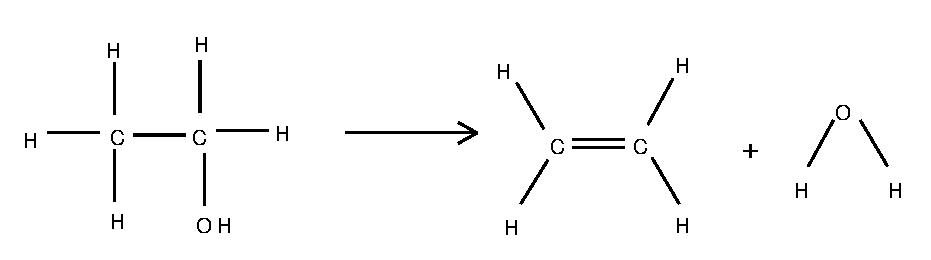
\includegraphics{../dehydration_alcohol.eps}
 % dehydration_alcohol.eps: 0x0 pixel, 300dpi, 0.00x0.00 cm, bb=9 14 440 123
\end{center}


 \begin{center}
 $\rm{CH_{3}CH_{2}OH \rightarrow CH_{2}CH_{2} + H_{2}O}$
 \end{center}
 
% \begin{center}
% \begin{pspicture}(-4,-2)(8,2)
% %\psgrid[gridcolor=lightgray]
% \rput(-4,0){\textbf{H}}
% \psline(-3.8,0)(-3.2,0)
% \rput(-3,0){\textbf{C}}
% \psline(-3,0.2)(-3,0.8)
% \rput(-3,1){\textbf{H}}
% \psline(-3,-0.2)(-3,-0.8)
% \rput(-3,-1){\textbf{H}}
% \rput(1,0){
% \psline(-3.8,0)(-3.2,0)
% \rput(-3,0){\textbf{C}}
% \psline(-3,0.2)(-3,0.8)
% \rput(-3,1){\textbf{H}}
% \psline(-3,-0.2)(-3,-0.8)
% \rput(-3,-1){\textbf{OH}}
% }
% 
% \psline(-1.8,0)(-1.2,0)
% \rput(-1,0){\textbf{H}}
% \psline[arrows=->](-0.6,0)(0.6,0)
% \rput(1,1){\textbf{H}}
% \rput(1,-1){\textbf{H}}
% \rput(2,0){\textbf{C}}
% \psline(1.8,0.3)(1.2,0.7)
% \psline(1.8,-0.3)(1.2,-0.7)
% \psline(2.2,0.05)(2.8,0.05)
% \psline(2.2,-0.05)(2.8,-0.05)
% \rput(3,0){\textbf{C}}
% \psline(3.2,0.3)(3.8,0.7)
% \psline(3.2,-0.3)(3.8,-0.7)
% \rput(4,1){\textbf{H}}
% \rput(4,-1){\textbf{H}}
% \rput(5,0){\textbf{+}}
% \rput(6,0){\textbf{H}}
% \psline(6.2,0)(6.8,0)
% \rput(7,0){\textbf{O}}
% \psline(7.2,0)(7.8,0)
% \rput(8,0){\textbf{H}}
% \psline(7,-0.2)(7,-0.8)
% \rput(7,-1){\textbf{H}}
% \end{pspicture}
% \end{center}
}

\item{The elimination of \textbf{potassium bromide from a bromoalkane}. 

\begin{center}
$\rm{CH_{3}CH_{2}Br + KOH \rightarrow CH_{2}CH_{2} + KBr + H_{2}O}$
\end{center}

\begin{center}
 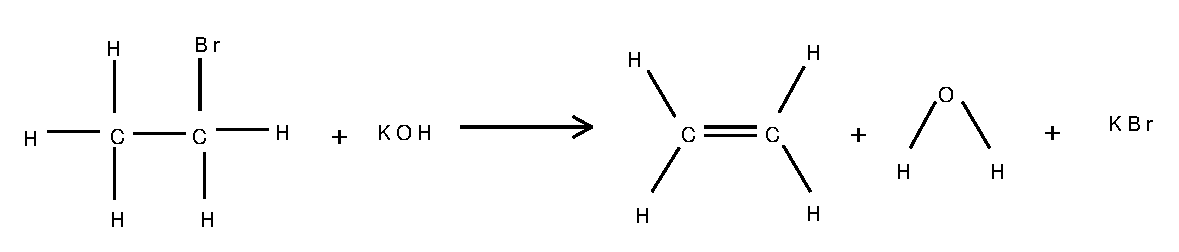
\includegraphics{../KBr_rearrange.eps}
 % KBr_rearrange.eps: 0x0 pixel, 300dpi, 0.00x0.00 cm, bb=9 15 559 120
\end{center}


% \begin{center}
% \begin{pspicture}(-6,-1.5)(6,1.5)
% \rput(-6,0){H}
% \psline(-5.7,0)(-5.3,0)
% \rput(-5,0){C}
% \psline(-5,0.3)(-5,0.7)
% \rput(-5,1){H}
% \psline(-5,-0.3)(-5,-0.7)
% \rput(-5,-1){H}
% \psline(-4.7,0)(-4.3,0)
% \rput(-4,0){C}
% \psline(-4,0.3)(-4,0.7)
% \rput(-4,1){Br}
% \psline(-4,-0.3)(-4,-0.7)
% \rput(-4,-1){H}
% \psline(-3.7,0)(-3.3,0)
% \rput(-3,0){H}
% \rput(-2.7,0){+}
% \rput(-2,0){KOH}
% \psline[arrows=->](-1.5,0)(-0.5,0)
% \rput(0,0){C}
% \psline(0,0.3)(0,0.7)
% \rput(0,1){H}
% \psline(0,-0.3)(0,-0.7)
% \rput(0,-1){H}
% \psline(0.3,0.05)(0.7,0.05)
% \psline(0.3,-0.05)(0.7,-0.05)
% \rput(1,0){
% \rput(0,0){C}
% \psline(0,0.3)(0,0.7)
% \rput(0,1){H}
% \psline(0,-0.3)(0,-0.7)
% \rput(0,-1){H}
% \rput(0.5,0){+}
% \rput(1.2,0){KBr}
% \rput(2,0){+}
% \rput(2.7,0){H$_{2}$O}
% }
% 
% 
% \end{pspicture}
% \end{center}

}

\item{Ethane cracking is an important industrial process used by SASOL and other petrochemical industries. Hydrogen is eliminated from ethane (C$_{2}$H$_{6}$) to produce an alkene called ethene (C$_{2}$H$_{4}$). Ethene is then used to produce other products such as polyethylene. You will learn more about these compounds in Grade 12. The equation for the cracking of ethane looks like this:

\begin{center}
$\rm{C_{2}H_{6} \rightarrow C_{2}H_{4} + H_{2}}$
\end{center}
}

\end{enumerate}

\subsection{Substitution reactions}

A substitution reaction occurs when an exchange of elements in the reactants takes place. The initial reactants are transformed or 'swopped around' to give a final product. A simple example of a reaction like this is shown below:

\begin{equation*}
AB + CD \rightarrow AC + BD
\end{equation*}

Some simple examples of substitution reactions are shown below:

\begin{equation*}
CH_{4} + Cl_{2} \rightarrow CH_{3}Cl + HCl
\end{equation*}

In this example, a chlorine atom and a hydrogen atom are exchanged to create a new product.

\begin{equation*}
Cu(H_{2}O)_{4}^{2+} + 4Cl^{-} \rightleftharpoons Cu(Cl)_{4}^{2-} + 4H_{2}O
\end{equation*}

In this example, four waters and four chlorines are exchanged to create a new product.

\Exercise{Addition, substitution and elimination reactions\\}{
\begin{enumerate}

\item{Refer to the diagram below and then answer the questions that follow:}
% \begin{center}
% \begin{pspicture}(-6,-1.5)(6,1.5)
% \rput(-6,-1.2){(i)}
% \rput(-6,0){H}
% \psline(-5.7,0)(-5.3,0)
% \rput(-5,0){C}
% \psline(-5,0.3)(-5,0.7)
% \rput(-5,1){H}
% \psline(-5,-0.3)(-5,-0.7)
% \rput(-5,-1){H}
% \psline(-4.7,0)(-4.3,0)
% \rput(-4,0){C}
% \psline(-4,0.3)(-4,0.7)
% \rput(-4,1){Cl}
% \psline(-4,-0.3)(-4,-0.7)
% \rput(-4,-1){H}
% \psline(-3.7,0)(-3.3,0)
% \rput(-3,0){H}
% \rput(-2.7,0){+}
% \rput(-2,0){KOH}
% \psline[arrows=->](-1.5,0)(-0.5,0)
% \rput(0,0){C}
% \psline(0,0.3)(0,0.7)
% \rput(0,1){H}
% \psline(0,-0.3)(0,-0.7)
% \rput(0,-1){H}
% \psline(0.3,0.05)(0.7,0.05)
% \psline(0.3,-0.05)(0.7,-0.05)
% \rput(1,0){
% \rput(0,0){C}
% \psline(0,0.3)(0,0.7)
% \rput(0,1){H}
% \psline(0,-0.3)(0,-0.7)
% \rput(0,-1){H}
% \rput(0.5,0){+}
% \rput(1.2,0){KCl}
% \rput(2,0){+}
% \rput(2.7,0){H$_{2}$O}
% }
% \end{pspicture}
% \end{center}

\begin{center}
 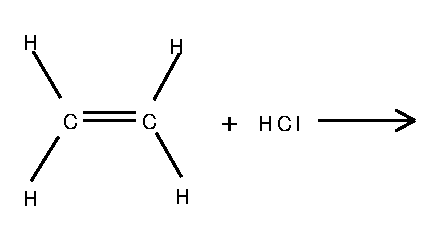
\includegraphics{../addition_rxn.eps}
 % addition_rxn.eps: 0x0 pixel, 300dpi, 0.00x0.00 cm, bb=7 8 203 104
\end{center}


	\begin{enumerate}
	\item{Is this reaction an example of substitution, elimination or addition?}
	\item{Give a reason for your answer above.}
	\end{enumerate}

\item{The following diagram shows the reactants in an addition reaction.}

% \begin{center}
% \begin{pspicture}(-6,-1.5)(6,1)
% 
% \rput(-5,0){
% \rput(0,0){C}
% \psline(0,0.3)(0,0.7)
% \rput(0,1){H}
% \psline(0,-0.3)(0,-0.7)
% \rput(0,-1){H}
% \psline(0.3,0.05)(0.7,0.05)
% \psline(0.3,-0.05)(0.7,-0.05)
% \rput(1,0){
% \rput(0,0){C}
% \psline(0,0.3)(0,0.7)
% \rput(0,1){H}
% \psline(0,-0.3)(0,-0.7)
% \rput(0,-1){H}
% \rput(0.5,0){+}
% \rput(1.2,0){HCl}
% \psline[arrows=->](2,0)(3,0)
% }
% }
% \end{pspicture}
% \end{center}

\begin{center}
 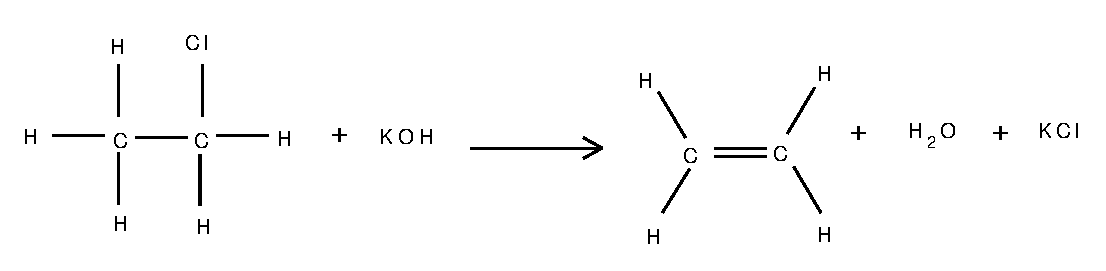
\includegraphics{../KCl_rearrange.eps}
 % KCl_rearrange.eps: 0x0 pixel, 300dpi, 0.00x0.00 cm, bb=4 4 519 118
\end{center}



	\begin{enumerate}
	\item{Draw the final product in this reaction.}
	\item{What is the chemical formula of the product?}
	\end{enumerate}

\item{The following reaction takes place:}

% \begin{center}
% \begin{pspicture}(-6,-1.5)(6,1)
% \rput(-6,0){H}
% \psline(-5.7,0)(-5.3,0)
% \rput(-5,0){C}
% \psline(-5,0.3)(-5,0.7)
% \rput(-5,1){H}
% \psline(-5,-0.3)(-5,-0.7)
% \rput(-5,-1){H}
% \psline(-4.7,0)(-4.3,0)
% \rput(-4,0){C}
% \psline(-4,0.3)(-4,0.7)
% \rput(-4,1){OH}
% \psline(-4,-0.3)(-4,-0.7)
% \rput(-4,-1){H}
% \psline(-3.7,0)(-3.3,0)
% \rput(-3,0){H}
% \rput(-1,0){
% \psline[arrows=->](-1.5,0)(-0.5,0)
% \rput(-1,0.2){H$_{2}$SO$_{4}$}
% \rput(0,0){C}
% \psline(0,0.3)(0,0.7)
% \rput(0,1){H}
% \psline(0,-0.3)(0,-0.7)
% \rput(0,-1){H}
% \psline(0.3,0.05)(0.7,0.05)
% \psline(0.3,-0.05)(0.7,-0.05)
% \rput(1,0){
% \rput(0,0){C}
% \psline(0,0.3)(0,0.7)
% \rput(0,1){H}
% \psline(0,-0.3)(0,-0.7)
% \rput(0,-1){H}
% \rput(0.5,0){+}
% \rput(1.2,0){H$_{2}$O}
% }
% }
% 
% \end{pspicture}
% \end{center}

\begin{center}
 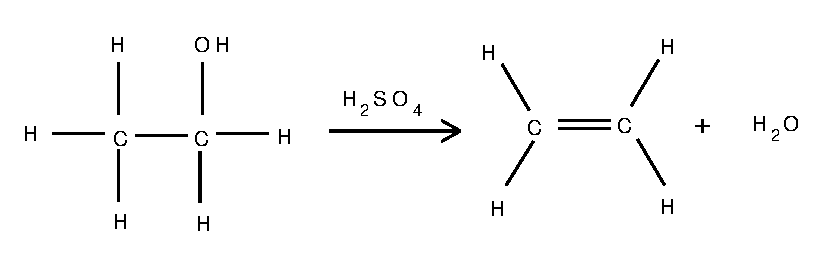
\includegraphics{../OH_rearrange.eps}
 % OH_rearrange.eps: 0x0 pixel, 300dpi, 0.00x0.00 cm, bb=4 6 387 113
\end{center}


Is this reaction a substitution, addition or dehydration reaction? Give a reason for your answer.

\item{
Consider the following reaction:
\begin{center}
$\rm{Ca(OH)_{2}(s) + 2NH_{4}Cl (s) \rightarrow CaCl_{2}(s) + 2NH_{3}(g) + 2H_{2}O(g)}$
\end{center}

Which one of the following best describes the type of reaction which takes place?
		\begin{enumerate}
		\item{Redox reaction}
		\item{Acid-base reaction}
		\item{Dehydration reaction}
		\end{enumerate}
}
\end{enumerate}
\practiceinfo
}
Presentation on types of reactions: SIYAVULA-PRESENTATION:http://cnx.org/content/m39090/latest/#slidesharefigure3
\summary{aaa}

\begin{itemize}
\item{There are many different \textbf{types of reactions} that can take place. These include acid-base, acid-carbonate, redox, addition, substitution and elimination reactions.}
\item{The \textbf{Arrhenius} definition of acids and bases defines an acid as a substance that increases the concentration of hydrogen ions (H$^{+}$ or H$_{3}$O$^{+}$) in a solution. A base is a substance that increases the concentration of hydroxide ions (OH$^{-}$) in a solution. However this definition only applies to substances that are in water.}
\item{The \textbf{Bronsted-Lowry} definition is a much broader one. An \textbf{acid} is a substance that \textbf{donates protons} and a \textbf{base} is a substance that \textbf{accepts protons}. }
\item{In different reactions, certain substances can act as both an acid and a base. These substances are called \textbf{ampholytes} and are said to be \textbf{amphoteric}. Water is an example of an amphoteric substance.}
\item{A \textbf{conjugate acid-base pair} refers to two compounds in a reaction (one reactant and one product) that transform or change into the other through the loss or gain of a proton.}
\item{When an acid and a base react, they form a \textbf{salt} and water. The salt is made up of a cation from the base and an anion from the acid. An example of a salt is sodium chloride (NaCl), which is the product of the reaction between sodium hydroxide (NaOH) and hydrochloric acid (HCl).}
\item{The reaction between an acid and a base is a \textbf{neutralisation} reaction.}
\item{\textbf{Titrations} are reactions between an acid and a base that are used to calculate the concentration of one of the reacting substances. The concentration of the other reacting substance must be known.}
\item{In an \textbf{acid-carbonate reaction}, an acid and a carbonate react to form a salt, carbon dioxide and water.}
\item{A \textbf{redox reaction} is one where there is always a change in the oxidation numbers of the elements that are involved in the reaction.}
\item{\textbf{Oxidation} is the loss of electrons and \textbf{reduction} is the gain of electrons.}
\item{When two or more reactants combine to form a product that contains all the atoms that were in the reactants, then this is an \textbf{addition reaction}. Examples of addition reactions include the reaction between ethene and bromine, polymerisation reactions and hydrogenation reactions.}
\item{A reaction where the reactant is broken down into one or more product, is called an \textbf{elimination reaction}. Alcohol dehydration and ethane cracking are examples of elimination reactions.}
\item{A \textbf{substitution reaction} is one where the reactants are transformed or swopped around to form the final product.}
\end{itemize}

\begin{eocexercises}{}
\begin{enumerate}
\item{
Give one word/term for each of the following descriptions:
	\begin{enumerate}
	\item{A chemical reaction during which electrons are transferred}
	\item{The addition of hydrogen across a double bond}
	\item{The removal of hydrogen and halogen atoms from an alkane to form an alkene}
	\end{enumerate}
}

\item{
For each of the following, say whether the statement is true or false. If the statement is false, re-write the statement correctly.
	\begin{enumerate}
	\item{The conjugate base of NH$_{4}^{+}$ is NH$_{3}$.}
	\item{The reactions $\rm{C + O_{2} \rightarrow CO_{2}}$ and $\rm{2KClO_{3} \rightarrow 2KCl + 3O_{2}}$ are examples of redox reactions.}
	\end{enumerate}
}

\item{For each of the following questions, choose the one correct statement from the list provided.}
\renewcommand{\labelenumii}{\Alph{enumii}}

	\begin{enumerate}
	\item{
The following chemical equation represents the formation of the hydronium ion:
	\begin{center}
	$\rm{H^{+} (aq) + H_{2}O (l) \rightarrow H_{3}O^{+} (aq)}$
	\end{center}

In this reaction, water acts as a Lewis base because it...
		\begin{enumerate}
		\item{accepts protons}
		\item{donates protons}
		\item{accepts electrons}
		\item{donates electrons}
		\end{enumerate}
}

(IEB Paper 2, 2005)

	\item{
When chlorine water (Cl$_{2}$ dissolved in water) is added to a solution of potassium bromide, bromine is produced. Which one of the following statements concerning this reaction is correct?
		\begin{enumerate}
		\item{Br$^{-}$ is oxidised}
		\item{Cl$_{2}$ is oxidised}
		\item{Br$^{-}$ is the oxidising agent}
		\item{Cl$^{-}$ is the oxidising agent}
		\end{enumerate}
}
(IEB Paper 2, 2005)
	\end{enumerate}
\renewcommand{\labelenumii}{\alph{enumii}}

\item{
The stomach secretes gastric juice, which contains hydrochloric acid. The gastric juice helps with digestion. Sometimes there is an overproduction of acid, leading to heartburn or indigestion. Antacids, such as milk of magnesia, can be taken to neutralise the excess acid. Milk of magnesia is only slightly soluble in water and has the chemical formula Mg(OH)$_{2}$.
	\begin{enumerate}
	\item{Write a balanced chemical equation to show how the antacid reacts with the acid.}
	\item{The directions on the bottle recommend that children under the age of 12 years take one teaspoon of milk of magnesia, whereas adults can take two teaspoons of the antacid. Briefly explain why the dosages are different.}
	\item{Why is it not advisable to take an overdose of the antacid in the stomach? Refer to the hydrochloric acid concentration in the stomach in your answer.}

\textit{In an experiment, 25.0 cm$^{3}$ of a standard solution of sodium carbonate of concentration 0.1 mol.dm$^{-3}$ was used to neutralise 35.0 cm$^{3}$ of a solution of hydrochloric acid.}

	\item{Write a balanced chemical equation for the reaction.}
	\item{Calculate the concentration of the acid.} 
	\end{enumerate}
}
(DoE Grade 11 Exemplar, 2007)
\end{enumerate}

\practiceinfo
\end{eocexercises}


% CHILD SECTION END 



% CHILD SECTION END 



% CHILD SECTION START 

\chapter{The Lithosphere}
\label{chap:lith}

%\nts{Need map showing major mining areas in SA}\\

% CHILD SECTION START 

\section{Introduction}
\label{sec:lith:intro}

If we were to cut the Earth in half we would see that our planet is made up of a number of layers, namely the \textbf{core} at the centre (seperated into the inner and outer core), the \textbf{mantle}, the \textbf{upper mantle}, the outer \textbf{crust} and the \textbf{atmosphere} (figure \ref{fig:earth section}). The core is made up mostly of iron. The mantle, which lies between the core and the crust, consists of molten rock, called \textbf{magma} which moves continuously because of convection currents. The crust is the thin, hard outer layer that 'floats' on the magma of the mantle. It is the upper part of the mantle and the crust that make up the \textbf{lithosphere} ('lith' means 'types of stone' and 'sphere' refers to the round shape of the earth). Together, the lithosphere, hydrosphere and atmosphere make up the world as we know it. \\

\begin{figure}[h]
\begin{center}
% \usepackage{pst-plot} % For axes
\scalebox{0.6} % Change this value to rescale the drawing.
{
\begin{pspicture}(0,-4.08)(23.94,9.181)
\pscircle[linewidth=0.04,dimen=outer](4.63,1.41){0.71}
\pscircle[linewidth=0.04,dimen=outer](4.63,1.39){1.59}
\pscircle[linewidth=0.04,dimen=outer](4.63,1.43){2.65}
\pscircle[linewidth=0.04,dimen=outer](4.63,1.43){3.51}
\pscircle[linewidth=0.04,dimen=outer](4.63,1.43){3.79}
\pscircle[linewidth=0.04,linestyle=dashed,dash=0.16cm 0.16cm,dimen=outer](4.65,1.39){4.65}
\psline[linewidth=0.04cm](10.44,4.18)(13.48,-2.46)
\psline[linewidth=0.04cm](13.44,-2.46)(16.44,4.34)
\psline[linewidth=0.04cm](13.52,-2.46)(16.32,-1.54)
\psline[linewidth=0.04cm](16.36,-1.54)(19.36,4.78)
\psline[linewidth=0.04cm](14.04,-1.22)(16.92,-0.42)
\psline[linewidth=0.04cm](14.4,-0.42)(17.24,0.34)
\psline[linewidth=0.04cm](15.28,1.62)(18.24,2.3)
\psline[linewidth=0.04cm](16.0,3.18)(18.92,3.7)
\psline[linewidth=0.04cm](16.12,3.46)(19.0,3.98)
\psline[linewidth=0.04cm](16.12,3.42)(16.04,3.42)
\psline[linewidth=0.04cm](15.48,-1.42)(19.64,-1.3)
\psline[linewidth=0.04cm](16.72,-0.18)(19.48,-0.1)
\psline[linewidth=0.04cm](17.08,1.5)(19.52,1.62)
\psline[linewidth=0.04cm](17.72,3.06)(19.56,3.1)
\psline[linewidth=0.04cm](18.48,3.74)(19.56,3.78)
\psline[linewidth=0.04cm](18.52,4.26)(19.56,4.3)
\usefont{T1}{ptm}{m}{n}
\rput(20.710938,-1.27){Inner Core}
\usefont{T1}{ptm}{m}{n}
\rput(20.808437,-0.03){Outer Core}
\usefont{T1}{ptm}{m}{n}
\rput(20.520937,1.69){Mantle}
\usefont{T1}{ptm}{m}{n}
\rput(20.931875,3.17){Upper Mantle}
\usefont{T1}{ptm}{m}{n}
\rput(20.321095,3.81){Crust}
\usefont{T1}{ptm}{m}{n}
\rput(20.836094,4.33){Atmosphere}
\psarc[linewidth=0.04](13.48,-1.7){0.68}{45.0}{135.0}
\psarc[linewidth=0.04](13.48,-1.58){1.52}{54.462322}{125.53768}
\psarc[linewidth=0.04](13.46,0.0){2.42}{42.455196}{139.28915}
\psarc[linewidth=0.04](13.54,0.32){3.78}{49.66686}{132.47388}
\psarc[linewidth=0.04](13.5,0.32){4.02}{51.241913}{131.53177}
\psarc[linewidth=0.04,linestyle=dashed,dash=0.16cm 0.16cm](13.56,0.78){4.6}{50.355824}{132.13759}
\psline[linewidth=0.04cm,linestyle=dashed,dash=0.16cm 0.16cm](16.48,4.3)(19.32,4.78)
\psarc[linewidth=0.04,linestyle=dashed,dash=0.16cm 0.16cm](15.14,0.76){5.78}{42.81836}{143.88066}
\psline[linewidth=0.04cm](4.6,1.34)(0.96,5.74)
\psline[linewidth=0.04cm](4.6,1.3)(4.96,6.9)
\psarc[linewidth=0.24200001,arrowsize=0.05291667cm 2.0,arrowlength=1.4,arrowinset=0.4]{<-<}(7.1,4.24){4.82}{24.968987}{155.90797}
\end{pspicture} 
}
\caption{A cross-section through the earth to show its different layers}
\label{fig:earth section}
\end{center}
\end{figure}


\Definition{Lithosphere}{The lithosphere is the solid outermost shell of our planet. The lithosphere includes the crust and the upper part of the mantle, and is made up of material from both the continents and the oceans on the Earth's surface.}


In grade 10 have focused on the hydrosphere and the atmosphere. The lithosphere is also very important, not only because it is the surface on which we live, but also because humans gain many valuable resources from this part of the planet. 


% CHILD SECTION END 



% CHILD SECTION START 

\section{The chemistry of the earth's crust}

The crust is made up of about 80 elements, which occur in over 2000 different compounds and minerals. However, most of the mass of the material in the crust is made up of only 8 of these elements. These are oxygen (O), silica (Si), aluminium (Al), iron (Fe), calcium (Ca), sodium (Na), potassium (K) and magnesium (Mg). These metal elements are seldom found in their pure form, but are usually part of other more complex \textbf{minerals}. A mineral is a compound that is formed through geological processes, which give it a particular structure. A mineral could be a pure element, but more often minerals are made up of many different elements combined. \textit{Quartz} is just one example. It is a mineral that is made up of silicon and oxygen. Some more examples are shown in table \ref{tab:minerals}. 

\Definition{Mineral}{Minerals are natural compounds formed through geological processes. The term 'mineral' includes both the material's chemical composition and its structure. Minerals range in composition from pure elements to complex compounds.}

\begin{table}[h]
\begin{center}
\caption{Table showing examples of minerals and their chemistry}
\label{tab:minerals}
\begin{tabular}{|l|p{4cm}|p{6cm}|}\hline
\textbf{Mineral} & \textbf{Chemistry} & \textbf{Comments}\\\hline
Quartz & SiO$_{2}$ (silicon dioxide) & Quartz is used for glass, in electrical components, optical lenses and in building stone \\\hline
Gold & Au (pure element) or AuTe$_{2}$ (Calaverite, a gold mineral) & Gold is often found in a group of minerals called the \textit{tellurides}. Calaverite is a mineral that belongs to this group, and is the most common gold-bearing mineral. Gold has an affinity for tellurium (Te). \\\hline
Hematite & Fe$_{2}$O$_{3}$ (iron oxide) & Iron usually occurs in iron oxide minerals or as an alloy of iron and nickel. \\\hline
Orthoclase & KAlSi$_{3}$O$_{8}$ (potassium aluminium silicate) & Orthoclase belongs to the \textit{feldspar} group of minerals. \\\hline
Copper & Cu (pure element) or Cu$_{2}$(CO$_{3}$)(OH)$_{2}$ (malachite or copper carbonate hydroxide) & copper can be mined as a pure element or as a mineral such as malachite. \\\hline
\end{tabular}
\end{center}
\end{table}

A \textbf{rock} is a combination of one or more minerals. \textit{Granite} for example, is a rock that is made up of minerals such as SiO$_{2}$, Al$_{2}$O$_{3}$, CaO, K$_{2}$O, Na$_{2}$O and others. There are three different types of rocks, \textbf{igneous}, \textbf{sedimentary} and \textbf{metamorphic}. Igneous rocks (e.g. granite, basalt) are formed when magma is brought to the earth's surface as lava, and then solidifies. Sedimentary rocks (e.g. sandstone, limestone) form when rock fragments, organic matter or other sediment particles are deposited and then compacted over time until they solidify. Metamorphic rock is formed when any other rock types are subjected to intense heat and pressure over a period of time. Examples include slate and marble.\\


Many of the elements that are of interest to us (e.g. gold, iron, copper), are unevenly distributed in the lithosphere. In places where these elements are abundant, it is profitable to extract them (e.g. through mining) for economic purposes. If their concentration is very low, then the cost of extraction becomes more than the money that would be made if they were sold. Rocks that contain valuable minerals are called \textbf{ores}. As humans, we are particularly interested in the ores that contain metal elements, and also in those minerals that can be used to produce energy. 

\Definition{Ore}{An ore is a volume of rock that contains minerals which make it valuable for mining.}

\begin{IFact}{
A \textbf{gemstone} (also sometimes called a \textbf{gem} or \textbf{semi-precious stone}), is a highly attractive and valuable piece of mineral which, when cut and polished, is used in jewelry and other adornments. Examples of gemstones are amethyst, diamond, cat's eye and sapphire.
}
\end{IFact}

\Exercise{Rocks and minerals\\}{
\begin{enumerate}
\item{Where are most of the earth's minerals concentrated?}
\item{Explain the difference between a \textit{mineral}, a \textit{rock} and an \textit{ore}.}
\item{Carry out your own research to find out which elements are found in the following minerals:
	\begin{enumerate}
	\item{gypsum}
	\item{calcite}
	\item{topaz}
	\end{enumerate}
}
\item{Which minerals are found in the following rocks?}
	\begin{enumerate}
	\item{basalt}
	\item{sandstone}
	\item{marble}
	\end{enumerate}
\end{enumerate}
\practiceinfo
}



% CHILD SECTION END 



% CHILD SECTION START 

\section{A brief history of mineral use}

Many of the minerals that are important to humans are \textbf{metals} such as gold, aluminium, copper and iron. Throughout history, metals have played a very important role in making jewelery, tools, weapons and later machinery and other forms of technology. We have become so used to having metals around us that we seldom stop to think what life might have been like before metals were discovered. During the \textbf{Stone Age} for example, \textbf{stones} were used to make tools. Slivers of stone were cut from a rock and then sharpened. In Africa, some of the stone tools that have been found date back to 2.5 million years ago! \\

It was the discovery of \textit{metals} that led to some huge advances in agriculture, warfare, transport and even cookery. One of the first metals to be discovered was \textbf{gold}, probably because of its beautiful shiny appearance. Gold was used mostly to make jewelery because it was too soft to make harder tools. Later, \textbf{copper} became an important metal because it could be hammered into shape, and it also lasted a lot longer than the stone that had previously been used in knives, cooking utensils and weapons. Copper can also be melted and then put into a mould to re-shape it. This is known as \textbf{casting}. \\

At about the time that copper was in widespread use, it was discovered that if certain kinds of stones are heated to high enough temperatures, liquid metals flow from them. These rocks are \textbf{ores}, and contain the metal minerals inside them. The process of heating mineral ores in this way is called \textbf{smelting}. It was also found that ores do not only occur at the earth's surface, but also deep \textit{below} it. This discovery led to the beginning of \textbf{mining}.\\

But humans' explorations into the world of metals did not end here! In some areas, the ores of \textit{iron} and \textit{tin} were found close together. The cast alloy of these two metals is \textbf{bronze}. Bronze is a very useful metal because it produces a sharper edge than copper. Another important discovery was that of \textbf{iron}. Iron is the most abundant metal at the earth's surface but it is more difficult to work with than copper or tin. It is very difficult to extract iron from its ore because it has an extremely high melting point, and only specially designed furnaces are able to produce the temperatures that are needed. An important discovery was that if iron is heated in a furnace with \textit{charcoal}, some of the carbon in the charcoal is transferred to the iron, making the metal even harder. If this hot metal has its temperature reduced very suddenly, it becomes even harder and produces \textbf{steel}. Today, steel is a very important part of industry and construction.\\


\begin{IFact}{
Originally it was believed that much of Africa's knowledge of metals and their uses was from the Middle East. But this may not be the case. More recent studies have shown that iron was used far earlier than it would have been if knowledge of this metal had started in the Middle East. Many metal technologies may in fact have developed independently in Africa and in many African countries, metals have an extremely important place in society. In Nigeria's Yoruba country for example, iron has divine status because it is used to make instruments for survival. 'Ogun', the God of Iron, is seen as the protector of the kingdom.
}
\end{IFact}




% CHILD SECTION END 



% CHILD SECTION START 

\section{Energy resources and their uses}
\label{sec:mining:energy}

Apart from minerals and ores, the products of the lithosphere are also important in meeting our energy needs.\\

\textbf{Coal} is one of the most important fuels that is used in the production of electricity. Coal is formed from organic material when plants and animals decompose, leaving behind organic remains that accumulate and become compacted over millions of years under sedimentary rock. The layers of compact organic material that can be found between sedimentary layers, are coal. When coal is burned, a large amount of heat energy is released, which is used to produce electricity. South Africa is the world's sixth largest coal producer, with Mpumalanga contributing about 83\% of our total production. Other areas in which coal is produced, include the Free State, Limpopo and KwaZulu-Natal. One of the problems with coal however, is that it is a non-renewable resource, meaning that once all resources have been used up, it cannot simply be produced again. Burning coal also produces large quantities of greenhouse gases, which may play a role in global warming. At present, ESKOM, the South African government's electric power producer, is the coal industry's main customer.\\

Another element that is found in the crust, and which helps to meet our energy needs, is \textbf{uranium}. Uranium produces energy through the process of \textit{nuclear fission}. Neutrons are aimed at the nucleii of the uranium atoms in order to split them. When the nucleus of a uranium atom is split, a large amount of energy is released as heat. This heat is used to produce steam, which turns turbines to generate electricity. Uranium is produced as a by-product of gold in some mines in the Witwatersrand, and as a by-product in some copper mines, for example in Phalaborwa. This type of nuclear power is relatively environmentally friendly since it produces low gas emissions. However, the process does produce small amounts of radioactive wastes , which must be carefully disposed of in order to prevent contamination.\\

\textbf{Oil} is another product of the lithosphere which is critical in meeting our fuel needs. While most of South Africa's oil is imported and then processed at a refinery in either Durban, Cape Town or Sasolburg, some is extracted from coal. The technology behind this type of extraction has largely been developed by SASOL (South African Coal, Oil and Gas Corporation). Oil, like coal, is organic in origin and normally forms from organic deposits on the ocean floor. Oil requires unique geological and geochemical conditions in order to be produced. Part of this process involves the burial of organic-rich sediments under extremely high temperatures and pressures. The oil that is produced is then pushed out into nearby sedimentary layers. Oil will then move upwards until it is trapped by an impermeable rock layer. It accumulates here, and can then be accessed by oil rigs and other advanced equipment.



% CHILD SECTION END 

\Activity{Research}{Mining Areas}{Using any reference resources you have available, try to find a map of the mining regions of South Africa.}

% CHILD SECTION START 

\section{Mining and Mineral Processing: Gold}

\subsection{Introduction}

Gold was discovered in South Africa in the late 1800's and since then has played a very important role in South Africa's \emph{history} and \emph{economy}. Its discovery brought many foreigners into South Africa, who were lured by the promises of wealth. They set up small mining villages, which later grew into larger settlements, towns and cities. One of the first of these settlements was the beginning of present-day Johannesburg, also known as 'Egoli' or 'Place of Gold'.\\

Most of South Africa's gold is concentrated in the 'Golden Arc', which stretches from Johannesburg to Welkom. Geologists believe that, millions of years ago, this area was a massive inland lake. Rivers feeding into this lake brought sand, silt, pebbles and fine particles of gold and deposited them over a long period of time. Eventually these deposits accumulated and became compacted to form gold-bearing sedimentary rock or \textbf{gold reefs}. It is because of this complex, but unique, set of circumstances that South Africa's gold deposits are so concentrated in that area. In other countries like Zimbabwe, gold occurs in smaller 'pockets', which are scattered over a much greater area.

\subsection{Mining the Gold}

A number of different techniques can be used to mine gold. The three most common methods in South Africa are \textbf{panning}, \textbf{open cast} and \textbf{shaft} mining.

\begin{enumerate}

\item{\textbf{Panning}

Panning for gold is a manual technique that is used to sort gold from other sediments. Wide, shallow pans are filled with sand and gravel (often from river beds) that may contain gold. Water is added and the pans are shaken so that the gold is sorted from the rock and other materials. Because gold is much more dense, it settles to the bottom of the pan. \textbf{Pilgrim's Rest} in Mpumalanga, was the first site for gold panning in South Africa.
}

\item{\textbf{Open cast mining}

This is a form of surface mining. Surface layers of rock and sediments are removed so that the deeper gold rich layers can be reached. This type of mining is not suitable if the gold is buried very deep below the surface.
}

\item{\textbf{Shaft mining}

South Africa's thin but extensive gold reefs slope at an angle underneath the ground, and this means that some deposits are very deep and often difficult to reach.  Shaft mining is needed to reach the gold ore. After the initial drilling, blasting and equipping of a mine shaft, tunnels are built leading outwards from the main shaft so that the gold reef can be reached. Shaft mining is a dangerous operation, and roof supports are needed so that the rock does not collapse. There are also problems of the intense heat and high pressure below the surface which make shaft mining very complex, dangerous and expensive. A diagram illustrating open cast and shaft mining is shown in figure \ref{fig:gold mining}.
}

\begin{figure}[h]
\begin{center}
% \usepackage{pst-plot} % For axes
\scalebox{1} % Change this value to rescale the drawing.
{
\begin{pspicture}(0,-5.183)(13.84,5.197)
\psline[linewidth=0.04cm](10.84,-2.263)(2.12,-2.243)
\pscustom[linewidth=0.04]
{
\newpath
\moveto(0.54,0.737)
\lineto(0.63,0.737)
\curveto(0.675,0.737)(0.745,0.737)(0.77,0.737)
\curveto(0.795,0.737)(0.855,0.737)(0.89,0.737)
\curveto(0.925,0.737)(1.085,0.717)(1.21,0.697)
\curveto(1.335,0.677)(1.505,0.652)(1.55,0.647)
\curveto(1.595,0.642)(1.675,0.632)(1.71,0.627)
\curveto(1.745,0.622)(1.805,0.617)(1.83,0.617)
\curveto(1.855,0.617)(1.905,0.607)(1.93,0.597)
\curveto(1.955,0.587)(2.015,0.572)(2.05,0.567)
\curveto(2.085,0.562)(2.16,0.552)(2.2,0.547)
\curveto(2.24,0.542)(2.315,0.532)(2.35,0.527)
\curveto(2.385,0.522)(2.455,0.502)(2.49,0.487)
\curveto(2.525,0.472)(2.605,0.447)(2.65,0.437)
\curveto(2.695,0.427)(2.79,0.407)(2.84,0.397)
\curveto(2.89,0.387)(2.975,0.372)(3.01,0.367)
\curveto(3.045,0.362)(3.105,0.352)(3.13,0.347)
\curveto(3.155,0.342)(3.21,0.322)(3.24,0.307)
\curveto(3.27,0.292)(3.335,0.262)(3.37,0.247)
\curveto(3.405,0.232)(3.48,0.197)(3.52,0.177)
\curveto(3.56,0.157)(3.625,0.122)(3.65,0.107)
\curveto(3.675,0.092)(3.725,0.057)(3.75,0.037)
\curveto(3.775,0.017)(3.84,-0.038)(3.88,-0.073)
\curveto(3.92,-0.108)(3.985,-0.153)(4.01,-0.163)
\curveto(4.035,-0.173)(4.085,-0.198)(4.11,-0.213)
\curveto(4.135,-0.228)(4.19,-0.253)(4.22,-0.263)
\curveto(4.25,-0.273)(4.295,-0.298)(4.31,-0.313)
\curveto(4.325,-0.328)(4.36,-0.368)(4.38,-0.393)
\curveto(4.4,-0.418)(4.435,-0.468)(4.45,-0.493)
\curveto(4.465,-0.518)(4.5,-0.568)(4.52,-0.593)
\curveto(4.54,-0.618)(4.58,-0.663)(4.6,-0.683)
\curveto(4.62,-0.703)(4.66,-0.738)(4.68,-0.753)
\curveto(4.7,-0.768)(4.745,-0.793)(4.77,-0.803)
\curveto(4.795,-0.813)(4.85,-0.833)(4.88,-0.843)
\curveto(4.91,-0.853)(4.96,-0.868)(4.98,-0.873)
\curveto(5.0,-0.878)(5.045,-0.883)(5.07,-0.883)
\curveto(5.095,-0.883)(5.15,-0.883)(5.18,-0.883)
\curveto(5.21,-0.883)(5.28,-0.883)(5.32,-0.883)
\curveto(5.36,-0.883)(5.435,-0.873)(5.47,-0.863)
\curveto(5.505,-0.853)(5.575,-0.838)(5.61,-0.833)
\curveto(5.645,-0.828)(5.705,-0.813)(5.73,-0.803)
\curveto(5.755,-0.793)(5.795,-0.773)(5.81,-0.763)
\curveto(5.825,-0.753)(5.865,-0.728)(5.89,-0.713)
\curveto(5.915,-0.698)(5.965,-0.658)(5.99,-0.633)
\curveto(6.015,-0.608)(6.055,-0.553)(6.07,-0.523)
\curveto(6.085,-0.493)(6.11,-0.443)(6.12,-0.423)
\curveto(6.13,-0.403)(6.15,-0.348)(6.16,-0.313)
\curveto(6.17,-0.278)(6.195,-0.213)(6.21,-0.183)
\curveto(6.225,-0.153)(6.255,-0.103)(6.27,-0.083)
\curveto(6.285,-0.063)(6.31,-0.023)(6.32,-0.0029999996)
\curveto(6.33,0.017)(6.36,0.052)(6.38,0.067)
\curveto(6.4,0.082)(6.44,0.107)(6.46,0.117)
\curveto(6.48,0.127)(6.525,0.147)(6.55,0.157)
\curveto(6.575,0.167)(6.61,0.192)(6.62,0.207)
\curveto(6.63,0.222)(6.66,0.252)(6.68,0.267)
\curveto(6.7,0.282)(6.745,0.307)(6.77,0.317)
\curveto(6.795,0.327)(6.845,0.337)(6.87,0.337)
\curveto(6.895,0.337)(6.95,0.342)(6.98,0.347)
\curveto(7.01,0.352)(7.065,0.362)(7.09,0.367)
\curveto(7.115,0.372)(7.16,0.392)(7.18,0.407)
\curveto(7.2,0.422)(7.25,0.457)(7.28,0.477)
\curveto(7.31,0.497)(7.36,0.527)(7.38,0.537)
\curveto(7.4,0.547)(7.445,0.567)(7.47,0.577)
\curveto(7.495,0.587)(7.55,0.597)(7.58,0.597)
\curveto(7.61,0.597)(7.685,0.602)(7.73,0.607)
\curveto(7.775,0.612)(7.85,0.627)(7.88,0.637)
\curveto(7.91,0.647)(7.965,0.657)(7.99,0.657)
\curveto(8.015,0.657)(8.07,0.657)(8.1,0.657)
\curveto(8.13,0.657)(8.2,0.657)(8.24,0.657)
\curveto(8.28,0.657)(8.355,0.652)(8.39,0.647)
\curveto(8.425,0.642)(8.485,0.637)(8.51,0.637)
\curveto(8.535,0.637)(8.59,0.627)(8.62,0.617)
\curveto(8.65,0.607)(8.71,0.592)(8.74,0.587)
\curveto(8.77,0.582)(8.825,0.577)(8.85,0.577)
\curveto(8.875,0.577)(8.925,0.577)(8.95,0.577)
\curveto(8.975,0.577)(9.03,0.577)(9.06,0.577)
\curveto(9.09,0.577)(9.145,0.582)(9.17,0.587)
\curveto(9.195,0.592)(9.245,0.602)(9.27,0.607)
\curveto(9.295,0.612)(9.345,0.617)(9.37,0.617)
\curveto(9.395,0.617)(9.45,0.617)(9.48,0.617)
\curveto(9.51,0.617)(9.565,0.622)(9.59,0.627)
\curveto(9.615,0.632)(9.67,0.637)(9.7,0.637)
\curveto(9.73,0.637)(9.785,0.637)(9.81,0.637)
\curveto(9.835,0.637)(9.89,0.637)(9.92,0.637)
\curveto(9.95,0.637)(10.005,0.637)(10.03,0.637)
\curveto(10.055,0.637)(10.12,0.637)(10.16,0.637)
\curveto(10.2,0.637)(10.27,0.637)(10.3,0.637)
\curveto(10.33,0.637)(10.395,0.637)(10.43,0.637)
\curveto(10.465,0.637)(10.525,0.637)(10.55,0.637)
\curveto(10.575,0.637)(10.62,0.642)(10.64,0.647)
\curveto(10.66,0.652)(10.7,0.657)(10.76,0.657)
}
\pscustom[linewidth=0.04]
{
\newpath
\moveto(4.32,-0.343)
\lineto(4.24,-0.363)
\curveto(4.2,-0.373)(4.135,-0.383)(4.11,-0.383)
\curveto(4.085,-0.383)(4.035,-0.388)(4.01,-0.393)
\curveto(3.985,-0.398)(3.93,-0.408)(3.9,-0.413)
\curveto(3.87,-0.418)(3.81,-0.428)(3.78,-0.433)
\curveto(3.75,-0.438)(3.69,-0.443)(3.66,-0.443)
\curveto(3.63,-0.443)(3.57,-0.448)(3.54,-0.453)
\curveto(3.51,-0.458)(3.45,-0.463)(3.42,-0.463)
\curveto(3.39,-0.463)(3.335,-0.463)(3.31,-0.463)
\curveto(3.285,-0.463)(3.235,-0.458)(3.21,-0.453)
\curveto(3.185,-0.448)(3.135,-0.443)(3.11,-0.443)
\curveto(3.085,-0.443)(3.04,-0.433)(3.02,-0.423)
\curveto(3.0,-0.413)(2.95,-0.388)(2.92,-0.373)
\curveto(2.89,-0.358)(2.835,-0.333)(2.81,-0.323)
\curveto(2.785,-0.313)(2.735,-0.303)(2.71,-0.303)
\curveto(2.685,-0.303)(2.64,-0.298)(2.62,-0.293)
\curveto(2.6,-0.288)(2.555,-0.283)(2.53,-0.283)
\curveto(2.505,-0.283)(2.46,-0.273)(2.44,-0.263)
\curveto(2.42,-0.253)(2.375,-0.243)(2.35,-0.243)
\curveto(2.325,-0.243)(2.275,-0.238)(2.25,-0.233)
\curveto(2.225,-0.228)(2.175,-0.218)(2.15,-0.213)
\curveto(2.125,-0.208)(2.075,-0.203)(2.05,-0.203)
\curveto(2.025,-0.203)(1.975,-0.208)(1.95,-0.213)
\curveto(1.925,-0.218)(1.88,-0.233)(1.86,-0.243)
\curveto(1.84,-0.253)(1.8,-0.268)(1.78,-0.273)
\curveto(1.76,-0.278)(1.715,-0.288)(1.69,-0.293)
\curveto(1.665,-0.298)(1.615,-0.313)(1.59,-0.323)
\curveto(1.565,-0.333)(1.515,-0.348)(1.49,-0.353)
\curveto(1.465,-0.358)(1.41,-0.363)(1.38,-0.363)
\curveto(1.35,-0.363)(1.29,-0.368)(1.26,-0.373)
\curveto(1.23,-0.378)(1.175,-0.388)(1.15,-0.393)
\curveto(1.125,-0.398)(1.075,-0.408)(1.05,-0.413)
\curveto(1.025,-0.418)(0.975,-0.423)(0.95,-0.423)
\curveto(0.925,-0.423)(0.875,-0.428)(0.85,-0.433)
\curveto(0.825,-0.438)(0.775,-0.438)(0.75,-0.433)
\curveto(0.725,-0.428)(0.675,-0.413)(0.65,-0.403)
\curveto(0.625,-0.393)(0.57,-0.368)(0.54,-0.353)
}
\pscustom[linewidth=0.04]
{
\newpath
\moveto(4.6,-0.703)
\lineto(4.52,-0.703)
\curveto(4.48,-0.703)(4.415,-0.708)(4.39,-0.713)
\curveto(4.365,-0.718)(4.32,-0.728)(4.3,-0.733)
\curveto(4.28,-0.738)(4.235,-0.748)(4.21,-0.753)
\curveto(4.185,-0.758)(4.135,-0.768)(4.11,-0.773)
\curveto(4.085,-0.778)(4.035,-0.788)(4.01,-0.793)
\curveto(3.985,-0.798)(3.935,-0.803)(3.91,-0.803)
\curveto(3.885,-0.803)(3.835,-0.808)(3.81,-0.813)
\curveto(3.785,-0.818)(3.735,-0.828)(3.71,-0.833)
\curveto(3.685,-0.838)(3.635,-0.843)(3.61,-0.843)
\curveto(3.585,-0.843)(3.535,-0.843)(3.51,-0.843)
\curveto(3.485,-0.843)(3.415,-0.843)(3.37,-0.843)
\curveto(3.325,-0.843)(3.255,-0.843)(3.23,-0.843)
\curveto(3.205,-0.843)(3.145,-0.843)(3.11,-0.843)
\curveto(3.075,-0.843)(3.01,-0.843)(2.98,-0.843)
\curveto(2.95,-0.843)(2.895,-0.838)(2.87,-0.833)
\curveto(2.845,-0.828)(2.8,-0.818)(2.78,-0.813)
\curveto(2.76,-0.808)(2.715,-0.798)(2.69,-0.793)
\curveto(2.665,-0.788)(2.615,-0.778)(2.59,-0.773)
\curveto(2.565,-0.768)(2.515,-0.763)(2.49,-0.763)
\curveto(2.465,-0.763)(2.415,-0.758)(2.39,-0.753)
\curveto(2.365,-0.748)(2.32,-0.738)(2.3,-0.733)
\curveto(2.28,-0.728)(2.24,-0.718)(2.22,-0.713)
\curveto(2.2,-0.708)(2.16,-0.698)(2.14,-0.693)
\curveto(2.12,-0.688)(2.07,-0.683)(2.04,-0.683)
\curveto(2.01,-0.683)(1.95,-0.678)(1.92,-0.673)
\curveto(1.89,-0.668)(1.835,-0.663)(1.81,-0.663)
\curveto(1.785,-0.663)(1.735,-0.663)(1.71,-0.663)
\curveto(1.685,-0.663)(1.635,-0.663)(1.61,-0.663)
\curveto(1.585,-0.663)(1.535,-0.663)(1.51,-0.663)
\curveto(1.485,-0.663)(1.44,-0.668)(1.42,-0.673)
\curveto(1.4,-0.678)(1.355,-0.693)(1.33,-0.703)
\curveto(1.305,-0.713)(1.255,-0.733)(1.23,-0.743)
\curveto(1.205,-0.753)(1.16,-0.773)(1.14,-0.783)
\curveto(1.12,-0.793)(1.075,-0.808)(1.05,-0.813)
\curveto(1.025,-0.818)(0.975,-0.828)(0.95,-0.833)
\curveto(0.925,-0.838)(0.87,-0.843)(0.84,-0.843)
\curveto(0.81,-0.843)(0.755,-0.848)(0.73,-0.853)
\curveto(0.705,-0.858)(0.655,-0.868)(0.63,-0.873)
\curveto(0.605,-0.878)(0.555,-0.888)(0.53,-0.893)
\curveto(0.505,-0.898)(0.465,-0.908)(0.42,-0.923)
}
\pscustom[linewidth=0.04]
{
\newpath
\moveto(6.18,-0.183)
\lineto(6.25,-0.193)
\curveto(6.285,-0.198)(6.335,-0.213)(6.35,-0.223)
\curveto(6.365,-0.233)(6.405,-0.248)(6.43,-0.253)
\curveto(6.455,-0.258)(6.51,-0.268)(6.54,-0.273)
\curveto(6.57,-0.278)(6.625,-0.288)(6.65,-0.293)
\curveto(6.675,-0.298)(6.73,-0.308)(6.76,-0.313)
\curveto(6.79,-0.318)(6.88,-0.323)(6.94,-0.323)
\curveto(7.0,-0.323)(7.105,-0.323)(7.15,-0.323)
\curveto(7.195,-0.323)(7.265,-0.323)(7.29,-0.323)
\curveto(7.315,-0.323)(7.365,-0.318)(7.39,-0.313)
\curveto(7.415,-0.308)(7.47,-0.298)(7.5,-0.293)
\curveto(7.53,-0.288)(7.59,-0.283)(7.62,-0.283)
\curveto(7.65,-0.283)(7.71,-0.278)(7.74,-0.273)
\curveto(7.77,-0.268)(7.825,-0.258)(7.85,-0.253)
\curveto(7.875,-0.248)(7.925,-0.238)(7.95,-0.233)
\curveto(7.975,-0.228)(8.02,-0.218)(8.04,-0.213)
\curveto(8.06,-0.208)(8.105,-0.203)(8.13,-0.203)
\curveto(8.155,-0.203)(8.215,-0.203)(8.25,-0.203)
\curveto(8.285,-0.203)(8.35,-0.203)(8.38,-0.203)
\curveto(8.41,-0.203)(8.465,-0.203)(8.49,-0.203)
\curveto(8.515,-0.203)(8.575,-0.203)(8.61,-0.203)
\curveto(8.645,-0.203)(8.715,-0.203)(8.75,-0.203)
\curveto(8.785,-0.203)(8.85,-0.203)(8.88,-0.203)
\curveto(8.91,-0.203)(8.97,-0.203)(9.0,-0.203)
\curveto(9.03,-0.203)(9.085,-0.203)(9.11,-0.203)
\curveto(9.135,-0.203)(9.19,-0.203)(9.22,-0.203)
\curveto(9.25,-0.203)(9.305,-0.203)(9.33,-0.203)
\curveto(9.355,-0.203)(9.405,-0.203)(9.43,-0.203)
\curveto(9.455,-0.203)(9.505,-0.203)(9.53,-0.203)
\curveto(9.555,-0.203)(9.61,-0.203)(9.64,-0.203)
\curveto(9.67,-0.203)(9.725,-0.203)(9.75,-0.203)
\curveto(9.775,-0.203)(9.825,-0.203)(9.85,-0.203)
\curveto(9.875,-0.203)(9.93,-0.208)(9.96,-0.213)
\curveto(9.99,-0.218)(10.045,-0.223)(10.07,-0.223)
\curveto(10.095,-0.223)(10.145,-0.233)(10.17,-0.243)
\curveto(10.195,-0.253)(10.245,-0.263)(10.27,-0.263)
\curveto(10.295,-0.263)(10.35,-0.268)(10.38,-0.273)
\curveto(10.41,-0.278)(10.465,-0.283)(10.49,-0.283)
\curveto(10.515,-0.283)(10.565,-0.283)(10.59,-0.283)
\curveto(10.615,-0.283)(10.665,-0.283)(10.69,-0.283)
\curveto(10.715,-0.283)(10.75,-0.283)(10.78,-0.283)
}
\pscustom[linewidth=0.04]
{
\newpath
\moveto(6.02,-0.583)
\lineto(6.07,-0.593)
\curveto(6.095,-0.598)(6.15,-0.608)(6.18,-0.613)
\curveto(6.21,-0.618)(6.265,-0.628)(6.29,-0.633)
\curveto(6.315,-0.638)(6.365,-0.643)(6.39,-0.643)
\curveto(6.415,-0.643)(6.47,-0.643)(6.5,-0.643)
\curveto(6.53,-0.643)(6.585,-0.643)(6.61,-0.643)
\curveto(6.635,-0.643)(6.685,-0.643)(6.71,-0.643)
\curveto(6.735,-0.643)(6.785,-0.643)(6.81,-0.643)
\curveto(6.835,-0.643)(6.885,-0.643)(6.91,-0.643)
\curveto(6.935,-0.643)(6.985,-0.648)(7.01,-0.653)
\curveto(7.035,-0.658)(7.08,-0.668)(7.1,-0.673)
\curveto(7.12,-0.678)(7.165,-0.688)(7.19,-0.693)
\curveto(7.215,-0.698)(7.265,-0.708)(7.29,-0.713)
\curveto(7.315,-0.718)(7.37,-0.723)(7.4,-0.723)
\curveto(7.43,-0.723)(7.5,-0.723)(7.54,-0.723)
\curveto(7.58,-0.723)(7.655,-0.723)(7.69,-0.723)
\curveto(7.725,-0.723)(7.79,-0.723)(7.82,-0.723)
\curveto(7.85,-0.723)(7.91,-0.723)(7.94,-0.723)
\curveto(7.97,-0.723)(8.095,-0.713)(8.19,-0.703)
\curveto(8.285,-0.693)(8.405,-0.683)(8.43,-0.683)
\curveto(8.455,-0.683)(8.51,-0.683)(8.54,-0.683)
\curveto(8.57,-0.683)(8.625,-0.683)(8.65,-0.683)
\curveto(8.675,-0.683)(8.74,-0.683)(8.78,-0.683)
\curveto(8.82,-0.683)(8.9,-0.678)(8.94,-0.673)
\curveto(8.98,-0.668)(9.08,-0.663)(9.14,-0.663)
\curveto(9.2,-0.663)(9.285,-0.663)(9.31,-0.663)
\curveto(9.335,-0.663)(9.385,-0.663)(9.41,-0.663)
\curveto(9.435,-0.663)(9.49,-0.663)(9.52,-0.663)
\curveto(9.55,-0.663)(9.605,-0.663)(9.63,-0.663)
\curveto(9.655,-0.663)(9.71,-0.663)(9.74,-0.663)
\curveto(9.77,-0.663)(9.825,-0.663)(9.85,-0.663)
\curveto(9.875,-0.663)(9.925,-0.663)(9.95,-0.663)
\curveto(9.975,-0.663)(10.025,-0.663)(10.05,-0.663)
\curveto(10.075,-0.663)(10.125,-0.663)(10.15,-0.663)
\curveto(10.175,-0.663)(10.225,-0.663)(10.25,-0.663)
\curveto(10.275,-0.663)(10.325,-0.663)(10.35,-0.663)
\curveto(10.375,-0.663)(10.425,-0.663)(10.45,-0.663)
\curveto(10.475,-0.663)(10.525,-0.663)(10.55,-0.663)
\curveto(10.575,-0.663)(10.625,-0.663)(10.65,-0.663)
\curveto(10.675,-0.663)(10.725,-0.663)(10.75,-0.663)
\curveto(10.775,-0.663)(10.81,-0.653)(10.84,-0.623)
}
\pscustom[linewidth=0.04]
{
\newpath
\moveto(0.6017364,-1.168705)
\lineto(0.7419229,-1.1756153)
\curveto(0.812016,-1.1790706)(0.92181915,-1.1873366)(0.96152896,-1.1921474)
\curveto(1.0012383,-1.1969582)(1.0707306,-1.2053767)(1.1005127,-1.2089851)
\curveto(1.1302948,-1.2125936)(1.199787,-1.2210121)(1.2394965,-1.2258229)
\curveto(1.2792059,-1.2306336)(1.3635888,-1.2408564)(1.4082624,-1.2462684)
\curveto(1.4529358,-1.2516804)(1.5224277,-1.2600996)(1.5472461,-1.2631062)
\curveto(1.5720649,-1.2661128)(1.6217017,-1.272126)(1.6465204,-1.2751325)
\curveto(1.6713392,-1.2781391)(1.720976,-1.2841536)(1.7457947,-1.2871602)
\curveto(1.7706131,-1.2901667)(1.8196487,-1.3011439)(1.843866,-1.3091145)
\curveto(1.8680832,-1.3170844)(1.9220825,-1.3286629)(1.9518646,-1.3322712)
\curveto(1.9816468,-1.3358797)(2.0362475,-1.3424946)(2.0610664,-1.3455012)
\curveto(2.085885,-1.3485078)(2.1299567,-1.3588837)(2.1492102,-1.3662525)
\curveto(2.1684637,-1.3736213)(2.2305865,-1.4012941)(2.2734559,-1.4215974)
\curveto(2.3163252,-1.4419001)(2.3840132,-1.4652107)(2.4088318,-1.4682173)
\curveto(2.43365,-1.4712238)(2.4826856,-1.4822011)(2.5069032,-1.4901717)
\curveto(2.5311205,-1.4981416)(2.5845184,-1.514684)(2.6136994,-1.5232557)
\curveto(2.6428802,-1.5318276)(2.696278,-1.5483699)(2.7204957,-1.5563399)
\curveto(2.744713,-1.5643104)(2.7981102,-1.5808527)(2.8272913,-1.5894246)
\curveto(2.8564723,-1.5979964)(2.910472,-1.6095747)(2.9352906,-1.6125813)
\curveto(2.9601088,-1.615588)(3.0147095,-1.6222029)(3.0444922,-1.6258113)
\curveto(3.0742743,-1.6294197)(3.1338384,-1.6366353)(3.1636207,-1.6402436)
\curveto(3.1934032,-1.643852)(3.2480042,-1.650467)(3.2728224,-1.6534736)
\curveto(3.297641,-1.6564802)(3.3472779,-1.6624935)(3.3720965,-1.6655)
\curveto(3.3969152,-1.6685066)(3.446552,-1.6745198)(3.471371,-1.6775264)
\curveto(3.4961889,-1.6805329)(3.5607178,-1.6883509)(3.6004272,-1.6931617)
\curveto(3.6401367,-1.6979725)(3.7145922,-1.7069929)(3.7493384,-1.7112019)
\curveto(3.7840846,-1.7154115)(3.848612,-1.7232295)(3.8783948,-1.7268373)
\curveto(3.908177,-1.730445)(3.967741,-1.7376618)(3.9975233,-1.7412697)
\curveto(4.027306,-1.7448775)(4.0918336,-1.7526954)(4.1265798,-1.7569051)
\curveto(4.1613255,-1.761114)(4.230818,-1.7695332)(4.265564,-1.7737422)
\curveto(4.30031,-1.7779511)(4.3747654,-1.7869716)(4.414475,-1.7917824)
\curveto(4.4541845,-1.7965932)(4.5286403,-1.8056135)(4.5633864,-1.8098226)
\curveto(4.598132,-1.8140321)(4.6582985,-1.8162849)(4.683718,-1.8143281)
\curveto(4.7091384,-1.8123714)(4.7699046,-1.8096602)(4.805252,-1.8089057)
\curveto(4.8405995,-1.8081514)(4.911294,-1.8066425)(4.9466414,-1.8058882)
\curveto(4.9819884,-1.8051338)(5.0427556,-1.8024226)(5.068176,-1.8004658)
\curveto(5.0935955,-1.798509)(5.143834,-1.7995589)(5.1686525,-1.8025655)
\curveto(5.193471,-1.805572)(5.273492,-1.8102297)(5.328694,-1.8118806)
\curveto(5.383896,-1.8135316)(5.4645176,-1.8132259)(5.489938,-1.811269)
\curveto(5.5153575,-1.8093122)(5.565596,-1.8103621)(5.590415,-1.8133687)
\curveto(5.615233,-1.8163753)(5.669834,-1.8229902)(5.699617,-1.826598)
\curveto(5.7293987,-1.8302058)(5.7988906,-1.838625)(5.8385997,-1.8434358)
\curveto(5.8783092,-1.8482466)(5.9478016,-1.8566657)(5.9775844,-1.8602736)
\curveto(6.007366,-1.8638813)(6.0718946,-1.8716993)(6.106641,-1.875909)
\curveto(6.1413865,-1.8801179)(6.210878,-1.8885372)(6.2456236,-1.8927461)
\curveto(6.2803698,-1.8969551)(6.344898,-1.9047725)(6.37468,-1.9083809)
\curveto(6.404463,-1.9119892)(6.4689903,-1.9198066)(6.5037365,-1.9240156)
\curveto(6.5384827,-1.9282253)(6.6179023,-1.9378468)(6.6625757,-1.9432588)
\curveto(6.7072487,-1.9486713)(6.7866673,-1.958293)(6.8214135,-1.962502)
\curveto(6.8561597,-1.9667115)(6.925652,-1.9751308)(6.9603977,-1.9793403)
\curveto(6.995144,-1.9835494)(7.0596714,-1.9913667)(7.089454,-1.9949751)
\curveto(7.1192365,-1.9985828)(7.173837,-2.0051973)(7.198656,-2.0082037)
\curveto(7.223474,-2.0112104)(7.2780747,-2.0178254)(7.3078575,-2.0214338)
\curveto(7.33764,-2.0250423)(7.402168,-2.0328596)(7.436914,-2.0370686)
\curveto(7.47166,-2.0412781)(7.5560427,-2.051501)(7.6056786,-2.0575147)
\curveto(7.6553164,-2.0635285)(7.7446632,-2.0743525)(7.7843723,-2.0791633)
\curveto(7.824082,-2.0839741)(7.893574,-2.0923927)(7.923357,-2.0960004)
\curveto(7.95314,-2.099609)(8.007739,-2.1062238)(8.032558,-2.1092305)
\curveto(8.057377,-2.112237)(8.111978,-2.1188521)(8.14176,-2.12246)
\curveto(8.171543,-2.1260676)(8.231106,-2.1332843)(8.260889,-2.1368923)
\curveto(8.290671,-2.1405)(8.354597,-2.1532815)(8.388742,-2.1624544)
\curveto(8.422887,-2.171628)(8.501704,-2.1862128)(8.546378,-2.1916256)
\curveto(8.591052,-2.1970375)(8.670471,-2.206659)(8.705217,-2.2108686)
\curveto(8.739964,-2.2150776)(8.804492,-2.222895)(8.834273,-2.2265034)
\curveto(8.864056,-2.2301118)(8.918656,-2.2367263)(8.943474,-2.2397327)
\curveto(8.968293,-2.2427394)(9.027858,-2.2499557)(9.062604,-2.2541645)
\curveto(9.09735,-2.2583742)(9.166241,-2.2717566)(9.200386,-2.2809298)
\curveto(9.23453,-2.2901032)(9.298457,-2.302884)(9.3282385,-2.3064923)
\curveto(9.35802,-2.3101008)(9.422549,-2.3179183)(9.457294,-2.322127)
\curveto(9.492041,-2.3263369)(9.551605,-2.333553)(9.576424,-2.3365595)
\curveto(9.601243,-2.3395662)(9.655842,-2.3461812)(9.685625,-2.3497896)
\curveto(9.715407,-2.3533978)(9.779937,-2.3612154)(9.814683,-2.3654244)
\curveto(9.849429,-2.369634)(9.908391,-2.381814)(9.932608,-2.3897846)
\curveto(9.956825,-2.3977547)(10.015789,-2.4099348)(10.050534,-2.4141438)
\curveto(10.08528,-2.4183533)(10.14981,-2.4261708)(10.179591,-2.4297786)
\curveto(10.2093725,-2.433387)(10.263973,-2.440002)(10.288792,-2.4430087)
\curveto(10.313611,-2.4460151)(10.363247,-2.4520283)(10.388066,-2.455035)
\curveto(10.412886,-2.4580414)(10.462522,-2.464056)(10.487341,-2.4670625)
\curveto(10.512159,-2.4700692)(10.56676,-2.476684)(10.596543,-2.4802918)
\curveto(10.626326,-2.4838996)(10.680925,-2.4905148)(10.705745,-2.4935212)
\curveto(10.730563,-2.496528)(10.760946,-2.4951727)(10.777641,-2.4820855)
}
\psdots[dotsize=0.12](0.52,-0.583)
\psdots[dotsize=0.12](0.74,-0.743)
\psdots[dotsize=0.12](0.84,-0.563)
\psdots[dotsize=0.12](0.94,-0.683)
\psdots[dotsize=0.12](1.1,-0.543)
\psdots[dotsize=0.12](1.14,-0.663)
\psdots[dotsize=0.12](1.34,-0.483)
\psdots[dotsize=0.12](1.46,-0.583)
\psdots[dotsize=0.12](1.62,-0.403)
\psdots[dotsize=0.12](1.78,-0.563)
\psdots[dotsize=0.12](1.86,-0.383)
\psdots[dotsize=0.12](2.08,-0.303)
\psdots[dotsize=0.12](2.0,-0.443)
\psdots[dotsize=0.12](1.96,-0.583)
\psdots[dotsize=0.12](2.18,-0.643)
\psdots[dotsize=0.12](2.16,-0.463)
\psdots[dotsize=0.12](2.32,-0.383)
\psdots[dotsize=0.12](2.48,-0.383)
\psdots[dotsize=0.12](2.44,-0.583)
\psdots[dotsize=0.12](2.6,-0.543)
\psdots[dotsize=0.12](2.76,-0.423)
\psdots[dotsize=0.12](2.9,-0.483)
\psdots[dotsize=0.12](2.8,-0.603)
\psdots[dotsize=0.12](2.68,-0.683)
\psdots[dotsize=0.12](2.88,-0.743)
\psdots[dotsize=0.12](2.98,-0.643)
\psdots[dotsize=0.12](3.08,-0.543)
\psdots[dotsize=0.12](3.3,-0.543)
\psdots[dotsize=0.12](3.14,-0.643)
\psdots[dotsize=0.12](3.26,-0.743)
\psdots[dotsize=0.12](3.46,-0.663)
\psdots[dotsize=0.12](3.6,-0.503)
\psdots[dotsize=0.12](3.6,-0.703)
\psdots[dotsize=0.12](3.7,-0.603)
\psdots[dotsize=0.12](3.82,-0.743)
\psdots[dotsize=0.12](3.9,-0.583)
\psdots[dotsize=0.12](3.98,-0.483)
\psdots[dotsize=0.12](4.04,-0.623)
\psdots[dotsize=0.12](4.28,-0.423)
\psdots[dotsize=0.12](4.24,-0.583)
\psdots[dotsize=0.12](4.38,-0.603)
\psdots[dotsize=0.12](6.16,-0.503)
\psdots[dotsize=0.12](6.38,-0.323)
\psdots[dotsize=0.12](6.56,-0.383)
\psdots[dotsize=0.12](6.54,-0.563)
\psdots[dotsize=0.12](6.76,-0.523)
\psdots[dotsize=0.12](6.86,-0.403)
\psdots[dotsize=0.12](7.0,-0.563)
\psdots[dotsize=0.12](7.1,-0.423)
\psdots[dotsize=0.12](7.18,-0.583)
\psdots[dotsize=0.12](7.34,-0.443)
\psdots[dotsize=0.12](7.62,-0.363)
\psdots[dotsize=0.12](7.52,-0.463)
\psdots[dotsize=0.12](7.4,-0.583)
\psdots[dotsize=0.12](7.54,-0.623)
\psdots[dotsize=0.12](7.78,-0.643)
\psdots[dotsize=0.12](8.0,-0.643)
\psdots[dotsize=0.12](7.8,-0.483)
\psdots[dotsize=0.12](7.94,-0.323)
\psdots[dotsize=0.12](8.0,-0.463)
\psdots[dotsize=0.12](8.14,-0.303)
\psdots[dotsize=0.12](8.4,-0.323)
\psdots[dotsize=0.12](8.26,-0.443)
\psdots[dotsize=0.12](8.18,-0.603)
\psdots[dotsize=0.12](8.42,-0.583)
\psdots[dotsize=0.12](8.66,-0.603)
\psdots[dotsize=0.12](8.52,-0.403)
\psdots[dotsize=0.12](8.74,-0.303)
\psdots[dotsize=0.12](8.76,-0.423)
\psdots[dotsize=0.12](8.96,-0.303)
\psdots[dotsize=0.12](8.94,-0.543)
\psdots[dotsize=0.12](9.2,-0.583)
\psdots[dotsize=0.12](9.06,-0.403)
\psdots[dotsize=0.12](9.28,-0.343)
\psdots[dotsize=0.12](9.44,-0.563)
\psdots[dotsize=0.12](9.44,-0.423)
\psdots[dotsize=0.12](9.58,-0.303)
\psdots[dotsize=0.12](9.66,-0.443)
\psdots[dotsize=0.12](9.8,-0.583)
\psdots[dotsize=0.12](9.78,-0.403)
\psdots[dotsize=0.12](9.9,-0.303)
\psdots[dotsize=0.12](9.92,-0.463)
\psdots[dotsize=0.12](10.12,-0.603)
\psdots[dotsize=0.12](10.1,-0.403)
\psdots[dotsize=0.12](10.32,-0.363)
\psdots[dotsize=0.12](10.28,-0.503)
\psdots[dotsize=0.12](10.42,-0.543)
\psdots[dotsize=0.12](10.62,-0.383)
\psdots[dotsize=0.12](10.72,-0.583)
\psdots[dotsize=0.12,dotangle=-6.907633](0.6889838,-1.2800063)
\psdots[dotsize=0.12,dotangle=-6.907633](0.6252203,-1.4737438)
\psdots[dotsize=0.12,dotangle=-6.907633](0.8165524,-1.5573621)
\psdots[dotsize=0.12,dotangle=-6.907633](0.818346,-1.3762633)
\psdots[dotsize=0.12,dotangle=-6.907633](1.0873039,-1.650602)
\psdots[dotsize=0.12,dotangle=-6.907633](1.029533,-1.462287)
\psdots[dotsize=0.12,dotangle=-6.907633](1.1853545,-1.3401408)
\psdots[dotsize=0.12,dotangle=-6.907633](1.297879,-1.5753816)
\psdots[dotsize=0.12,dotangle=-6.907633](1.379092,-1.4039043)
\psdots[dotsize=0.12,dotangle=-6.907633](1.5313262,-1.6439558)
\psdots[dotsize=0.12,dotangle=-6.907633](1.43988,-1.7336085)
\psdots[dotsize=0.12,dotangle=-6.907633](1.6907766,-1.8244429)
\psdots[dotsize=0.12,dotangle=-6.907633](1.5427413,-1.3834378)
\psdots[dotsize=0.12,dotangle=-6.907633](1.689553,-1.5019549)
\psdots[dotsize=0.12,dotangle=-6.907633](1.8429691,-1.3996636)
\psdots[dotsize=0.12,dotangle=-6.907633](1.7298745,-1.6680096)
\psdots[dotsize=0.12,dotangle=-6.907633](1.8808851,-1.5855732)
\psdots[dotsize=0.12,dotangle=-6.907633](2.0144465,-1.4808766)
\psdots[dotsize=0.12,dotangle=-6.907633](2.138386,-1.4555992)
\psdots[dotsize=0.12,dotangle=-6.907633](2.077028,-1.6294819)
\psdots[dotsize=0.12,dotangle=-6.907633](1.9458722,-1.7143236)
\psdots[dotsize=0.12,dotangle=-6.907633](2.0108593,-1.8430742)
\psdots[dotsize=0.12,dotangle=-6.907633](2.2292624,-1.8695334)
\psdots[dotsize=0.12,dotangle=-6.907633](2.2557216,-1.6511303)
\psdots[dotsize=0.12,dotangle=-6.907633](2.4265869,-1.5710992)
\psdots[dotsize=0.12,dotangle=-6.907633](2.4049385,-1.7497927)
\psdots[dotsize=0.12,dotangle=-6.907633](2.4548814,-1.836428)
\psdots[dotsize=0.12,dotangle=-6.907633](2.6089094,-1.8953809)
\psdots[dotsize=0.12,dotangle=-6.907633](2.5535438,-1.687211)
\psdots[dotsize=0.12,dotangle=-6.907633](2.7743523,-1.6938154)
\psdots[dotsize=0.12,dotangle=-6.907633](2.7352545,-1.8502486)
\psdots[dotsize=0.12,dotangle=-6.907633](2.8844717,-1.948911)
\psdots[dotsize=0.12,dotangle=-6.907633](3.0102048,-1.7425348)
\psdots[dotsize=0.12,dotangle=-6.907633](3.0854251,-1.95311)
\psdots[dotsize=0.12,dotangle=-6.907633](3.2141757,-1.8881229)
\psdots[dotsize=0.12,dotangle=-6.907633](3.3080273,-1.7786155)
\psdots[dotsize=0.12,dotangle=-6.907633](3.350754,-1.9248154)
\psdots[dotsize=0.12,dotangle=-6.907633](3.4157412,-2.053566)
\psdots[dotsize=0.12,dotangle=-6.907633](3.5168087,-1.8844941)
\psdots[dotsize=0.12,dotangle=-6.907633](3.6852689,-1.8243178)
\psdots[dotsize=0.12,dotangle=-6.907633](3.6636205,-2.0030112)
\psdots[dotsize=0.12,dotangle=-6.907633](3.5673635,-2.1323736)
\psdots[dotsize=0.12,dotangle=-6.907633](3.7635064,-2.1762822)
\psdots[dotsize=0.12,dotangle=-6.907633](3.8026044,-2.0198488)
\psdots[dotsize=0.12,dotangle=-6.907633](3.861557,-1.865821)
\psdots[dotsize=0.12,dotangle=-6.907633](4.0029464,-1.8628039)
\psdots[dotsize=0.12,dotangle=-6.907633](4.318218,-1.9211448)
\psdots[dotsize=0.12,dotangle=-6.907633](4.156974,-1.9217566)
\psdots[dotsize=0.12,dotangle=-6.907633](3.9271557,-2.1558156)
\psdots[dotsize=0.12,dotangle=-6.907633](4.1509814,-2.3038092)
\psdots[dotsize=0.12,dotangle=-6.907633](4.19489,-2.1076663)
\psdots[dotsize=0.12,dotangle=-6.907633](4.4499855,-1.997547)
\psdots[dotsize=0.12,dotangle=-6.907633](4.6009965,-1.9151105)
\psdots[dotsize=0.12,dotangle=-6.907633](4.4632363,-2.2207608)
\psdots[dotsize=0.12,dotangle=-6.907633](4.3314686,-2.1443586)
\psdots[dotsize=0.12,dotangle=-6.907633](4.317036,-2.2634876)
\psdots[dotsize=0.12,dotangle=-6.907633](4.674423,-2.3067846)
\psdots[dotsize=0.12,dotangle=-6.907633](4.636507,-2.120875)
\psdots[dotsize=0.12,dotangle=-6.907633](4.77969,-1.936759)
\psdots[dotsize=0.12,dotangle=-6.907633](4.9433393,-1.9162923)
\psdots[dotsize=0.12,dotangle=-6.907633](4.881981,-2.0901752)
\psdots[dotsize=0.12,dotangle=-6.907633](4.904853,-2.2339697)
\psdots[dotsize=0.12,dotangle=-6.907633](5.0835466,-2.255618)
\psdots[dotsize=0.12,dotangle=-6.907633](5.0408196,-2.1094182)
\psdots[dotsize=0.12,dotangle=-6.907633](5.139482,-1.960201)
\psdots[dotsize=0.12,dotangle=-6.907633](5.3055367,-1.9198796)
\psdots[dotsize=0.12,dotangle=-6.907633](5.561244,-1.9710044)
\psdots[dotsize=0.12,dotangle=-6.907633](5.3308144,-2.0438192)
\psdots[dotsize=0.12,dotangle=-6.907633](5.4752207,-2.1821914)
\psdots[dotsize=0.12,dotangle=-6.907633](5.2670507,-2.2375567)
\psdots[dotsize=0.12,dotangle=-6.907633](5.673769,-2.2062452)
\psdots[dotsize=0.12,dotangle=-6.907633](5.912027,-2.2351098)
\psdots[dotsize=0.12,dotangle=-6.907633](6.1352406,-2.2218592)
\psdots[dotsize=0.12,dotangle=-6.907633](6.336194,-2.2260582)
\psdots[dotsize=0.12,dotangle=-6.907633](6.614162,-2.2597337)
\psdots[dotsize=0.12,dotangle=-6.907633](6.909579,-2.315669)
\psdots[dotsize=0.12,dotangle=-6.907633](5.8217626,-1.9824195)
\psdots[dotsize=0.12,dotangle=-6.907633](5.8470397,-2.1063592)
\psdots[dotsize=0.12,dotangle=-6.907633](6.1123686,-2.0780647)
\psdots[dotsize=0.12,dotangle=-6.907633](6.3554373,-2.0672197)
\psdots[dotsize=0.12,dotangle=-6.907633](6.5118704,-2.1063175)
\psdots[dotsize=0.12,dotangle=-6.907633](6.7675776,-2.1574423)
\psdots[dotsize=0.12,dotangle=-6.907633](7.0106463,-2.1465971)
\psdots[dotsize=0.12,dotangle=-6.907633](7.0756335,-2.2753477)
\psdots[dotsize=0.12,dotangle=-6.907633](7.2091947,-2.170651)
\psdots[dotsize=0.12,dotangle=-6.907633](7.269371,-2.339111)
\psdots[dotsize=0.12,dotangle=-6.907633](7.3830776,-2.2320092)
\psdots[dotsize=0.12,dotangle=-6.907633](7.5936527,-2.1567888)
\psdots[dotsize=0.12,dotangle=-6.907633](7.5124397,-2.3282661)
\psdots[dotsize=0.12,dotangle=-6.907633](7.398733,-2.4353683)
\psdots[dotsize=0.12,dotangle=-6.907633](6.6628814,-2.023881)
\psdots[dotsize=0.12,dotangle=-6.907633](7.5924706,-2.4991317)
\psdots[dotsize=0.12,dotangle=-6.907633](7.6490183,-2.3649585)
\psdots[dotsize=0.12,dotangle=-6.907633](7.8517656,-2.1880589)
\psdots[dotsize=0.12,dotangle=-6.907633](8.169442,-2.2265449)
\psdots[dotsize=0.12,dotangle=-6.907633](8.020838,-2.2891266)
\psdots[dotsize=0.12,dotangle=-6.907633](7.9570737,-2.4828641)
\psdots[dotsize=0.12,dotangle=-6.907633](7.817478,-2.3047824)
\psdots[dotsize=0.12,dotangle=-6.907633](7.7934246,-2.5033307)
\psdots[dotsize=0.12,dotangle=-6.907633](8.106291,-2.5815265)
\psdots[dotsize=0.12,dotangle=-6.907633](8.352377,-2.7120705)
\psdots[dotsize=0.12,dotangle=-6.907633](8.242257,-2.456975)
\psdots[dotsize=0.12,dotangle=-6.907633](8.440194,-2.3197846)
\psdots[dotsize=0.12,dotangle=-6.907633](8.423356,-2.4587686)
\psdots[dotsize=0.12,dotangle=-6.907633](8.665813,-2.2866795)
\psdots[dotsize=0.12,dotangle=-6.907633](8.92152,-2.3378043)
\psdots[dotsize=0.12,dotangle=-6.907633](8.830687,-2.5887008)
\psdots[dotsize=0.12,dotangle=-6.907633](8.635155,-2.706036)
\psdots[dotsize=0.12,dotangle=-6.907633](8.621904,-2.4828224)
\psdots[dotsize=0.12,dotangle=-6.907633](8.873413,-2.7349007)
\psdots[dotsize=0.12,dotangle=-6.907633](9.03164,-2.5928998)
\psdots[dotsize=0.12,dotangle=-6.907633](8.735611,-2.3757203)
\psdots[dotsize=0.12,dotangle=-6.907633](9.299375,-2.5447505)
\psdots[dotsize=0.12,dotangle=-6.907633](9.530416,-2.6331797)
\psdots[dotsize=0.12,dotangle=-6.907633](10.550228,-2.6962895)
\psdots[dotsize=0.12,dotangle=-6.907633](10.319186,-2.6078606)
\psdots[dotsize=0.12,dotangle=-6.907633](9.956988,-2.6042733)
\psdots[dotsize=0.12,dotangle=-6.907633](9.701282,-2.5531485)
\psdots[dotsize=0.12,dotangle=-6.907633](9.830032,-2.4881616)
\psdots[dotsize=0.12,dotangle=-6.907633](9.512355,-2.4496753)
\psdots[dotsize=0.12,dotangle=-6.907633](9.245233,-2.6590686)






\psdots[dotsize=0.12,dotangle=-6.907633](9.097809,-2.3793075)
\psdots[dotsize=0.12,dotangle=-6.907633](10.701239,-2.6138532)
\psdots[dotsize=0.12,dotangle=-6.907633](10.085739,-2.5392864)
\psdots[dotsize=0.12,dotangle=-6.907633](6.025121,-1.9667637)
\psdots[dotsize=0.12,dotangle=-6.907633](9.805978,-2.6867096)
\psdots[dotsize=0.12,dotangle=-6.907633](1.2190715,-1.727004)
\psdots[dotsize=0.12,dotangle=-6.907633](0.9844008,-1.3359419)
\psdots[dotsize=0.12,dotangle=-6.907633](0.88153946,-1.6861126)
\psdots[dotsize=0.12,dotangle=-6.907633](0.58131164,-1.6698867)
\psdots[dotsize=0.12](6.32,-0.503)
\psline[linewidth=0.04cm](10.76,0.657)(10.76,-0.083)
\psline[linewidth=0.04cm](10.8,-0.923)(10.82,-2.243)
\psline[linewidth=0.04cm](10.84,-3.223)(10.86,-5.083)
\psline[linewidth=0.04cm](11.78,0.797)(11.86,-5.163)
\pscustom[linewidth=0.04]
{
\newpath
\moveto(11.76,0.777)
\lineto(11.82,0.807)
\curveto(11.85,0.822)(11.91,0.847)(11.94,0.857)
\curveto(11.97,0.867)(12.02,0.882)(12.04,0.887)
\curveto(12.06,0.892)(12.115,0.897)(12.15,0.897)
\curveto(12.185,0.897)(12.27,0.902)(12.32,0.907)
\curveto(12.37,0.912)(12.485,0.907)(12.55,0.897)
\curveto(12.615,0.887)(12.74,0.842)(12.8,0.807)
\curveto(12.86,0.772)(12.985,0.687)(13.05,0.637)
\curveto(13.115,0.587)(13.2,0.507)(13.22,0.477)
\curveto(13.24,0.447)(13.275,0.397)(13.29,0.377)
\curveto(13.305,0.357)(13.335,0.322)(13.35,0.307)
\curveto(13.365,0.292)(13.4,0.292)(13.42,0.307)
\curveto(13.44,0.322)(13.475,0.347)(13.49,0.357)
\curveto(13.505,0.367)(13.535,0.397)(13.55,0.417)
\curveto(13.565,0.437)(13.595,0.467)(13.61,0.477)
\curveto(13.625,0.487)(13.655,0.507)(13.67,0.517)
\curveto(13.685,0.527)(13.725,0.537)(13.75,0.537)
\curveto(13.775,0.537)(13.805,0.542)(13.82,0.557)
}
\psline[linewidth=0.04cm](10.74,-0.042999998)(6.22,-0.163)
\psline[linewidth=0.04cm](10.8,-0.963)(6.12,-1.043)
\psline[linewidth=0.04cm](6.12,-1.043)(6.12,-0.563)
\pscustom[linewidth=0.04]
{
\newpath
\moveto(0.51453096,-1.7222352)
\lineto(0.60387754,-1.7330592)
\curveto(0.64855105,-1.7384712)(0.7478253,-1.7504976)(0.80242616,-1.7571125)
\curveto(0.857027,-1.7637275)(0.9414099,-1.7739509)(0.971192,-1.7775587)
\curveto(1.0009742,-1.7811666)(1.0500097,-1.7921443)(1.0692633,-1.7995131)
\curveto(1.0885168,-1.8068818)(1.1325891,-1.8172578)(1.1574075,-1.8202645)
\curveto(1.182226,-1.823271)(1.2312618,-1.8342488)(1.2554791,-1.8422188)
\curveto(1.279696,-1.8501893)(1.3336957,-1.8617684)(1.3634778,-1.8653761)
\curveto(1.3932599,-1.8689839)(1.4478607,-1.8755989)(1.4726795,-1.8786055)
\curveto(1.4974979,-1.8816121)(1.547135,-1.8876264)(1.5719534,-1.8906331)
\curveto(1.5967718,-1.8936397)(1.6513727,-1.9002546)(1.6811551,-1.9038625)
\curveto(1.7109375,-1.9074702)(1.7804291,-1.9158894)(1.8201388,-1.9207002)
\curveto(1.8598486,-1.925511)(1.9343042,-1.9345307)(1.9690499,-1.9387398)
\curveto(2.0037959,-1.9429493)(2.068324,-1.9507673)(2.0981064,-1.9543751)
\curveto(2.1278887,-1.9579829)(2.187453,-1.9651997)(2.2172353,-1.9688075)
\curveto(2.2470179,-1.9724153)(2.31651,-1.9808345)(2.3562195,-1.9856453)
\curveto(2.3959289,-1.9904561)(2.460457,-1.9982735)(2.485276,-2.00128)
\curveto(2.510094,-2.0042865)(2.564695,-2.0109017)(2.5944777,-2.01451)
\curveto(2.6242597,-2.0181184)(2.67886,-2.0247328)(2.7036786,-2.0277393)
\curveto(2.7284973,-2.030746)(2.793025,-2.0385633)(2.832735,-2.043374)
\curveto(2.872445,-2.0481849)(2.9419367,-2.0566034)(2.9717188,-2.060212)
\curveto(3.0015008,-2.0638204)(3.0561018,-2.0704353)(3.0809205,-2.073442)
\curveto(3.1057386,-2.0764484)(3.155376,-2.0824616)(3.1801941,-2.0854683)
\curveto(3.2050128,-2.0884748)(3.2633746,-2.1056185)(3.2969177,-2.1197553)
\curveto(3.3304615,-2.1338923)(3.3888233,-2.1510358)(3.4136415,-2.1540425)
\curveto(3.43846,-2.1570492)(3.4874964,-2.168027)(3.5117133,-2.1759968)
\curveto(3.5359302,-2.1839674)(3.5794013,-2.1993074)(3.5986547,-2.2066762)
\curveto(3.6179078,-2.2140448)(3.6564147,-2.2287836)(3.6756682,-2.2361524)
\curveto(3.694922,-2.2435212)(3.7389941,-2.2538972)(3.7638123,-2.256904)
\curveto(3.7886305,-2.2599103)(3.837666,-2.270888)(3.8618836,-2.2788582)
\curveto(3.886101,-2.2868288)(3.939499,-2.3033712)(3.96868,-2.3119428)
\curveto(3.9978607,-2.3205147)(4.0518603,-2.332093)(4.0766783,-2.3350997)
\curveto(4.101497,-2.3381062)(4.1610622,-2.345323)(4.195808,-2.349532)
\curveto(4.230554,-2.3537416)(4.300045,-2.3621607)(4.334791,-2.3663704)
\curveto(4.3695374,-2.3705792)(4.429102,-2.3777955)(4.453921,-2.3808022)
\curveto(4.478739,-2.3838086)(4.5283766,-2.3898225)(4.5531945,-2.3928292)
\curveto(4.5780125,-2.3958356)(4.633816,-2.3925228)(4.664801,-2.3862038)
\curveto(4.695786,-2.3798847)(4.752191,-2.3716085)(4.7776113,-2.3696516)
\curveto(4.803031,-2.3676949)(4.8588343,-2.3643818)(4.8892183,-2.3630257)
\curveto(4.919602,-2.36167)(4.974804,-2.363321)(4.999623,-2.3663275)
\curveto(5.024441,-2.3693342)(5.1050634,-2.369029)(5.1608667,-2.365716)
\curveto(5.21667,-2.3624036)(5.318349,-2.3545759)(5.364225,-2.3500605)
\curveto(5.4101014,-2.345545)(5.4764333,-2.3384712)(5.4968896,-2.3359132)
\curveto(5.5173464,-2.3333552)(5.583077,-2.3312452)(5.628351,-2.331694)
\curveto(5.673626,-2.3321419)(5.7393565,-2.3300326)(5.7598133,-2.3274739)
\curveto(5.7802696,-2.3249152)(5.8255444,-2.3253634)(5.850363,-2.3283699)
\curveto(5.875181,-2.3313766)(5.92542,-2.3324263)(5.95084,-2.3304694)
\curveto(5.9762597,-2.3285127)(6.0370264,-2.3258016)(6.072374,-2.325047)
\curveto(6.107721,-2.3242927)(6.1784153,-2.3227847)(6.2137628,-2.32203)
\curveto(6.24911,-2.3212757)(6.3148413,-2.3191657)(6.3452244,-2.3178103)
\curveto(6.375608,-2.3164546)(6.4314117,-2.3131416)(6.4568315,-2.311185)
\curveto(6.4822516,-2.309228)(6.5324903,-2.310278)(6.557308,-2.3132844)
\curveto(6.582127,-2.316291)(6.636728,-2.322906)(6.66651,-2.3265145)
\curveto(6.696293,-2.3301227)(6.7552557,-2.3423023)(6.7844367,-2.3508742)
\curveto(6.8136177,-2.3594458)(6.8769436,-2.3771906)(6.9110875,-2.3863642)
\curveto(6.945232,-2.3955371)(7.018485,-2.4144843)(7.0575933,-2.4242592)
\curveto(7.0967016,-2.4340339)(7.1687517,-2.4629085)(7.2016935,-2.4820087)
\curveto(7.234636,-2.5011091)(7.2961574,-2.5337458)(7.324736,-2.547281)
\curveto(7.353316,-2.560816)(7.4110765,-2.5829237)(7.4402575,-2.5914955)
\curveto(7.4694386,-2.6000674)(7.5432935,-2.614051)(7.5879664,-2.6194637)
\curveto(7.632639,-2.6248755)(7.7219872,-2.6356995)(7.76666,-2.6411116)
\curveto(7.811333,-2.6465242)(7.890752,-2.6561458)(7.925498,-2.6603549)
\curveto(7.960244,-2.6645644)(8.019208,-2.6767445)(8.043426,-2.684715)
\curveto(8.067641,-2.6926851)(8.116677,-2.7036622)(8.141497,-2.7066689)
\curveto(8.166315,-2.7096753)(8.225277,-2.721855)(8.259421,-2.7310286)
\curveto(8.293567,-2.7402015)(8.3618555,-2.7585475)(8.396001,-2.7677205)
\curveto(8.430145,-2.776894)(8.498434,-2.79524)(8.532578,-2.8044136)
\curveto(8.566724,-2.8135865)(8.635013,-2.8319325)(8.669158,-2.8411055)
\curveto(8.703302,-2.850279)(8.777156,-2.8642628)(8.816865,-2.8690736)
\curveto(8.856575,-2.8738844)(8.926067,-2.882303)(8.95585,-2.8859115)
\curveto(8.985632,-2.8895197)(9.040232,-2.8961349)(9.065051,-2.8991413)
\curveto(9.0898695,-2.902148)(9.154397,-2.9099653)(9.194106,-2.914776)
\curveto(9.233816,-2.919587)(9.323164,-2.9304109)(9.3728,-2.9364247)
\curveto(9.422438,-2.9424384)(9.506822,-2.9526606)(9.541568,-2.9568703)
\curveto(9.576313,-2.9610798)(9.635877,-2.9682953)(9.660696,-2.971302)
\curveto(9.685515,-2.9743085)(9.745078,-2.9815254)(9.779824,-2.9857345)
\curveto(9.81457,-2.989944)(9.903917,-3.000768)(9.958518,-3.0073824)
\curveto(10.013119,-3.0139973)(10.112392,-3.0260248)(10.157066,-3.0314374)
\curveto(10.20174,-3.0368502)(10.271232,-3.045268)(10.29605,-3.0482748)
\curveto(10.320869,-3.0512812)(10.380433,-3.0584981)(10.415179,-3.062707)
\curveto(10.449925,-3.066916)(10.52002,-3.0703719)(10.5553665,-3.0696175)
\curveto(10.590713,-3.0688632)(10.642756,-3.0550215)(10.659451,-3.0419343)
\curveto(10.676145,-3.0288472)(10.703369,-3.0119991)(10.734956,-3.0007164)
}
\psdots[dotsize=0.12,dotangle=-6.907633](9.144164,-2.8281405)
\psdots[dotsize=0.12,dotangle=-6.907633](9.411899,-2.7799914)
\psdots[dotsize=0.12,dotangle=-6.907633](9.727171,-2.8383322)
\psdots[dotsize=0.12,dotangle=-6.907633](10.195859,-2.7943819)
\psdots[dotsize=0.12,dotangle=-6.907633](10.484059,-2.9098818)
\psdots[dotsize=0.12,dotangle=-6.907633](10.285511,-2.885828)
\psdots[dotsize=0.12,dotangle=-6.907633](9.908269,-2.8401258)
\psdots[dotsize=0.12,dotangle=-6.907633](9.543666,-2.8563933)
\psdots[dotsize=0.12,dotangle=-6.907633](10.67478,-2.832256)
\psdots[dotsize=0.12,dotangle=-6.907633](10.042442,-2.8966732)
\psdots[dotsize=0.12,dotangle=-6.907633](10.401623,-2.758871)
\psdots[dotsize=0.12,dotangle=-6.907633](10.620638,-2.9465744)
\psline[linewidth=0.04cm](10.82,-3.263)(2.16,-3.203)
\psline[linewidth=0.04cm](2.14,-2.243)(2.16,-3.243)
\pscircle[linewidth=0.04,dimen=inner](1.14,-0.042999998){0.3}
\pscircle[linewidth=0.04,dimen=inner](5.18,-0.563){0.28}
\pscircle[linewidth=0.04,dimen=inner](4.16,-1.483){0.24}
\pscircle[linewidth=0.04,dimen=inner](11.35,-1.473){0.25}
\pscircle[linewidth=0.04,dimen=inner](6.21,-2.813){0.29}
\usefont{T1}{ptm}{m}{n}
\rput(1.0895313,-0.073){1}
\usefont{T1}{ptm}{m}{n}
\rput(5.177969,-0.573){2}
\usefont{T1}{ptm}{m}{n}
\rput(4.1357813,-1.513){3}
\usefont{T1}{ptm}{m}{n}
\rput(11.332188,-1.493){4}
\usefont{T1}{ptm}{m}{n}
\rput(6.170625,-2.813){5}
\pscircle[linewidth=0.04,dimen=inner](0.37,3.867){0.27}
\usefont{T1}{ptm}{m}{n}
\rput(0.32953125,3.867){1}
\pscircle[linewidth=0.04,dimen=inner](0.37,3.207){0.27}
\usefont{T1}{ptm}{m}{n}
\rput(0.33796874,3.207){2}
\pscircle[linewidth=0.04,dimen=inner](0.36,2.537){0.28}
\usefont{T1}{ptm}{m}{n}
\rput(0.33578125,2.527){3}
\pscircle[linewidth=0.04,dimen=inner](0.37,1.887){0.27}
\usefont{T1}{ptm}{m}{n}
\rput(0.3521875,1.867){4}
\pscircle[linewidth=0.04,dimen=inner](0.39,1.247){0.29}
\usefont{T1}{ptm}{m}{n}
\rput(0.370625,1.207){5}
\usefont{T1}{ptm}{m}{n}
\rput(3.3284376,3.847){Gold seam close to surface}
\usefont{T1}{ptm}{m}{n}
\rput(4.3825,3.187){Open cast mining at shallow gold seam}
\usefont{T1}{ptm}{m}{n}
\rput(2.6892188,2.607){Sloping gold seams}
\usefont{T1}{ptm}{m}{n}
\rput(4.364375,1.307){Tunnel from main shaft to access gold}
\usefont{T1}{ptm}{m}{n}
\rput(3.1135938,1.907){Main underground shaft}
\psframe[linewidth=0.04,dimen=inner](0.8,5.157)(0.0,4.397)
\psdots[dotsize=0.092](0.1,5.037)
\psdots[dotsize=0.092](0.34,5.057)
\psdots[dotsize=0.092](0.2,4.837)
\psdots[dotsize=0.092](0.44,4.717)
\psdots[dotsize=0.092](0.4,4.977)
\psdots[dotsize=0.092](0.58,5.077)
\psdots[dotsize=0.092](0.58,4.817)
\psdots[dotsize=0.092](0.66,4.977)
\psdots[dotsize=0.092](0.64,4.637)
\psdots[dotsize=0.092](0.48,4.517)
\psdots[dotsize=0.092](0.66,4.517)
\psdots[dotsize=0.092](0.1,4.677)
\psdots[dotsize=0.092](0.28,4.737)
\psdots[dotsize=0.092](0.24,4.517)
\psdots[dotsize=0.092](0.08,4.477)
\psdots[dotsize=0.092](0.68,4.797)
\psdots[dotsize=0.092](0.4,4.817)
\psdots[dotsize=0.092](0.2,4.977)
\psdots[dotsize=0.092](0.72,5.117)
\psdots[dotsize=0.092](0.32,4.437)
\psdots[dotsize=0.092](0.32,4.637)
\usefont{T1}{ptm}{m}{n}
\rput(2.16875,4.747){Gold deposits}
\end{pspicture} 
}
\caption{Diagram showing open cast and shaft mining}
\label{fig:gold mining}
\end{center}
\end{figure}


\end{enumerate}

\subsection{Processing the gold ore}

For every ton of ore that is mined, only a very small amount of gold is extracted. A number of different methods can be used to separate gold from its ore, but one of the more common methods is called \textbf{gold cyanidation}.\\

In the process of gold cyanidation, the ore is crushed and then cyanide (CN$^{-}$) solution is added so that the gold particles are chemically dissolved from the ore. In this step of the process, gold is oxidised. Zinc dust is then added to the cyanide solution. The zinc takes the place of the gold, so that the gold is precipitated out of the solution. This process is shown in figure \ref{fig:gold:processing}.

\begin{figure}[h]
\begin{center}
\begin{pspicture}(-7,-2.5)(7,7)
%\psgrid[gridcolor=lightgray]
\rput(0,6){\textbf{STEP 1} - The ore is crushed until it is in fine pieces}
\psline[linewidth=1pt,arrows=->](0,5.6)(0,4.6)
\rput(0,4){\textbf{STEP 2} - A sodium cyanide (NaCN) solution is mixed with the finely ground rock}
\rput(0,3.5){\rm${4Au + 8NaCN + O_{2} + 2H_{2}O \rightarrow 4NaAu(CN)_{2} + 4NaOH}$}
\rput(0,3){Gold is \textbf{oxidised}.}
\psline[linewidth=1pt,arrows=->](0,2.5)(0,2)
\rput(0,1.5){\textbf{STEP 3} - The gold-bearing solution can then be separated from the}
\rput(0,1){remaining solid ore through filtration}
\psline[linewidth=1pt,arrows=->](0,0.5)(0,-0.5)
\rput(0,-1){\textbf{STEP 4} - Zinc is added. Zinc replaces the gold in the gold-cyanide solution.}
\rput(0,-1.5){The gold is precipitated from the solution.}
\rput(0,-2){This is the \textbf{reduction} part of the reaction.}
\end{pspicture}
\caption{Flow diagram showing how gold is processed}
\label{fig:gold:processing}
\end{center}
\end{figure}

\begin{IFact}{
Another method that is used to process gold is called the 'carbon-in-pulp' (CIP) method. This method makes use of the high affinity that activated carbon has for gold, and there are three stages to the process. The first stage involves the \emph{absorption} of gold in the cyanide solution to carbon. In the \emph{elution} stage, gold is removed from the carbon into an alkaline cyanide solution. In the final stage, \emph{electro-winning} is used to remove gold from the solution through a process of electrolysis. Gold that has been removed is deposited on steel wool electrodes. The carbon is then treated so that it can be re-used.}
\end{IFact}

\subsection{Characteristics and uses of gold}
Gold has a number of uses because of its varied and unique characteristics. Below is a list of some of these characteristics that have made gold such a valuable metal:
\begin{itemize}

\item \emph{Shiny}

Gold's beautiful appearance has made it one of the favourite metals for use in jewelery.

\item \emph{Durable}

Gold does not tarnish or corrode easily, and therefore does not deteriorate in quality. It is sometimes used in dentistry to make the crowns for teeth.

\item \emph{Malleable and ductile}

Since gold can be bent and twisted into shape, as well as being flattened into very thin sheets, it is very useful in fine wires and to produce sheets of gold. 

\item \emph{Good conductor}

Gold is a good conductor of electricity and is therefore used in transistors, computer circuits and telephone exchanges.

\item \emph{Heat ray reflector}

Because gold reflects heat very effectively, it is used in space suits and in vehicles. It is also used in the protective outer coating of artificial satellites. One of the more unusual applications of gold is its use in firefighting, where a thin layer of gold is placed in the masks of the firefighters to protect them from the heat.

\end{itemize}

\Activity{Case Study}{Dropping like a gold balloon\\}{
Read the article below, which has been adapted from one that appeared in the \textit{Financial Mail} on 15th April 2005 and then answer the questions that follow.\\

\begin{quote}{
As recently as 1980, South Africa accounted for over 70\% of world gold production. In 2004, that figure was a dismal 14\%. Chamber of Mines figures showed that SA's annual gold production last year slipped to its lowest level since 1931.

Chamber economist Roger Baxter says the 'precipitous' fall in production was caused by the dual impact of the fall in the rand gold price due to the strong rand, and the continued upward rise in costs. Many of these costs, laments Baxter, are 'costs we do not have control over'. These include water, transport, steel and labour costs, which rose by 13\% on average in 2004.

He provides a breakdown of the cost components faced by mines:
\begin{itemize}
\item{Water prices have risen by 10\% per year for the past 3 years}
\item{Steel prices have increased by double-digit rates for each of the past 3 years}
\item{Spoornet's tariffs rose 35\% in 2003 and 16.5\% in 2004}
\item{Labour costs, which make up 50\% of production costs, rose above inflation in 2003 and 2004}
\end{itemize}
}

At these costs, and at current rand gold prices, about 10 mines, employing 90 000 people, are marginal or loss-making, says Baxter.
\end{quote}

\begin{enumerate}
\item{Refer to the table below showing SA's gold production in tons between 1980 and 2004.
\begin{center}
\begin{tabular}{|p{2cm}|p{2cm}|}\hline
\textbf{Year} & \textbf{Production (t)}\\\hline
1980 & 675 \\\hline
1985 & 660 \\\hline
1990 & 600 \\\hline
1995 & 525 \\\hline
2000 & 425 \\\hline
2004 & 340 \\\hline
\end{tabular}
\end{center}

Draw a line graph to illustrate these statistics.}

\item{What percentage did South Africa's gold production contribute towards global production in:
\begin{enumerate}
\item{1980}
\item{2004}
\end{enumerate}
}
\item{Outline two reasons for this drop in gold production.}
\item{Briefly explain how the increased cost of resources such as water contributes towards declining profitability in gold mines.}
\item{Suggest a reason why the cost of \textit{steel} might affect gold production.}
\item{Suggest what impact a decrease in gold production is likely to have on...
\begin{enumerate}
\item{South Africa's economy}
\item{mine employees}
\end{enumerate}
}
\item{Find out what the current price of gold is. Discuss why you think gold is so expensive.}

\end{enumerate}
}

\subsection{Environmental impacts of gold mining}
However, despite the incredible value of gold and its usefulness in a variety of applications, all mining has an environmental cost. The following are just a few of the environmental impacts of gold mining:

\begin{itemize}
\item{\textit{Resource consumption}

Gold mining needs large amounts of electricity and water.
}

\item{\textit{Poisoned water}

Acid from gold processing can leach into nearby water systems such as rivers, causing damage to animals and plants, as well as humans that may rely on that water for drinking. The disposal of other toxic waste (e.g. cyanide) can also have a devastating effect on biodiversity.
}

\item{\textit{Solid waste}

This applies particularly to open pit mines, where large amounts of soil and rock must be displaced in order to access the gold reserves. Processing the gold ore also leaves solid waste behind.
}

\item{\textit{Air pollution}

Dust from open pit mines, as well as harmful gases such as sulfur dioxide and nitrogen dioxide which are released from the furnaces, contribute to air pollution.
}

\item{\textit{Threaten natural areas}

Mining activities often encroach on protected areas and threaten biodiversity in their operation areas.
}
\end{itemize}

\Activity{Discussion}{Mine rehabilitation\\}{

There is a growing emphasis on the need to rehabilitate old mine sites that are no longer in use. If it is too difficult to restore the site to what it was before, then a new type of land use might be decided for that area. Any mine rehabilitation programme should aim to achieve the following:\\

\begin{itemize}
\item{ensure that the site is safe and stable}
\item{remove pollutants that are contaminating the site}
\item{restore the biodiversity that was there before mining started}
\item{restore waterways to what they were before mining\\}
\end{itemize}

There are different ways to achieve these goals. Plants for example, can be used to remove metals from polluted soils and water, and can also help to stabilise the soil so that other vegetation can grow. Land contouring can help to restore drainage in the area.\\

\textbf{Discussion:}\\

\textit{In groups of 3-4, discuss the following questions:}\\

\begin{enumerate}
\item{What are the main benefits of mine rehabilitation?}
\item{What are some of the difficulties that may be experienced in trying to rehabilitate a mine site?}
\item{Suggest some creative ideas that could be used to encourage mining companies to rehabilitate old sites.}
\item{One rehabilitation project that has received a lot of publicity is the rehabilitation of dunes that were mined for titanium by Richards Bay Minerals (RBM). As a group, carry out your own research to try to find out more about this project.}
	\begin{itemize}
	\item{What actions did RBM take to rehabilitate the dunes?}
	\item{Was the project successful?}
	\item{What were some of the challenges faced?}
	\end{itemize}
\end{enumerate}
}

\Exercise{Gold mining\\}{
Mapungubwe in the Limpopo Province is evidence of gold mining in South Africa as early as 1200. Today, South Africa is a world leader in the technology of gold mining. The following flow diagram illustrates some of the most important steps in the recovery of gold from its ore.

\begin{center}
\begin{pspicture}(-6,-1.4)(6,0.8)
\psframe(-5.8,-1)(-3.3,0.5)
\rput(-4.5,0){Gold}
\rput(-4.5,-0.3){bearing ore}

\psframe(-2.8,-1)(-0.3,0.5)
\rput(-1.5,0){NaAu(CN)$_{2}$}

\psframe(0.2,-1)(2.7,0.5)
\rput(1.5,0){Gold}
\rput(1.5,-0.3){precipitate}

\psframe(3.2,-1)(5.7,0.5)
\rput(4.5,0){Pure gold}

\psline[arrows=->,linewidth=2pt](-3.3,-0.25)(-2.8,-0.25)
\rput(-3,0){\textbf{A}}
\psline[arrows=->,linewidth=2pt](-0.3,-0.25)(0.2,-0.25)
\rput(0,0){\textbf{B}}
\psline[arrows=->,linewidth=2pt](2.7,-0.25)(3.2,-0.25)
\rput(3,0){\textbf{C}}

\end{pspicture} 
\end{center}

\begin{enumerate}
\item{Name the process indicated by A.}
\item{During process A, gold is extracted from the ore. Is gold oxidised or reduced during this process?}
\item{Use oxidation numbers to explain your answer to the question above.}
\item{Name the chemical substance that is used in process B.}
\item{During smelting (illustrated by C in the diagram), gold is sent into a calcining furnace. Briefly explain the importance of this process taking place in the furnace.}
\item{The recovery of gold can have a negative impact on water in our country, if not managed properly. State at least one negative influence that the recovery of gold can have on water resources and how it will impact on humans and the environment.}  
\end{enumerate}
\practiceinfo
}



% CHILD SECTION END 



% CHILD SECTION START 

\section{Mining and mineral processing: Iron}
\label{sec:mining:iron}

Iron is one of the most abundant metals on Earth. Its concentration is highest in the core, and lower in the crust. It is extracted from \textbf{iron ore} and is almost never found in its elemental form. Iron ores are usually rich in \textbf{iron oxide} minerals and may vary in colour from dark grey to rusty red. Iron is usually found in minerals such as magnetite (Fe$_{3}$O$_{4}$) and hematite (Fe$_{2}$O$_{3}$). Iron ore also contains other elements, which have to be removed in various ways. These include silica (Si), phosphorus (P), aluminium (Al) and sulfur (S).

\subsection{Iron mining and iron ore processing}

One of the more common methods of mining for iron ore is \textbf{open cast mining}. Open cast mining is used when the iron ore is found near the surface. Once the ore has been removed, it needs to be crushed into fine particles before it can be processed further.\\

As mentioned earlier, iron is commonly found in the form of \textbf{iron oxides}. To create pure iron, the ore must be \textbf{smelted} to remove the oxygen. 

\Definition{Smelting}{
Smelting is a method used to extract a metal from its ore and then purify it.
}

Smelting usually involves heating the ore and also adding a reducing agent (e.g. carbon) so that the metal can be freed from its ore. The bonds between iron and oxygen are very strong, and therefore it is important to use an element that will form stronger bonds with oxygen that the iron. This is why carbon is used. In fact, carbon monoxide is the main ingredient that is needed to strip oxygen from iron. These reactions take place in a \textbf{blast furnace}.\\

A blast furnace is a huge steel container many metres high and lined with heat-resistant material. In the furnace the solid raw materials, i.e. iron ore, carbon (in the form of 'coke', a type of coal) and a flux (e.g. limestone) are fed into the top of the furnace and a blast of heated air is forced into the furnace from the bottom. Temperatures in a blast furnace can reach 2000$^{\degree}$C. A simple diagram of a blast furnace is shown in figure \ref{fig:blast furnace}. The equations for the reactions that take place are shown in the flow diagram below. \\

\begin{center}

STEP 1: Production of carbon monoxide\\

\rm${C + O_{2} \rightarrow CO_{2}}$

\rm${CO_{2} + C \rightarrow 2CO}$
\end{center}

\begin{center}
STEP 2: Reduction of iron oxides takes place in a number of stages to produce iron.\\

\rm${3Fe_{2}O_{3} + CO \rightarrow 2Fe_{3}O_{4} + CO_{2}}$

\rm${Fe_{3}O_{4} + CO \rightarrow 3FeO + CO_{2}}$

\rm${FeO + CO \rightarrow Fe + CO_{2}}$
\end{center} 

\begin{center}
STEP 3: Fluxing

The flux is used to melt impurities in the ore. A common flux is limestone (CaCO$_{3}$). Common impurities are silica, phosphorus (makes steel brittle), aluminium and sulfur (produces SO$_{2}$ gases during smelting and interferes with the smellting process).\\


\rm${CaCO_{3} \rightarrow CaO + CO_{2}}$

\rm${CaO + SiO_{2} \rightarrow CaSiO_{3}}$
\end{center}

In step 3, the calcium carbonate breaks down into calcium oxide and carbon dioxide. The calcium oxide then reacts with silicon dioxide (the impurity) to form a \textbf{slag}. In this case the slag is the CaSiO$_{3}$. The slag melts in the furnace, whereas the silicon dioxide would not have, and floats on the more dense iron. This can then be separated and removed.

\begin{figure}[h]
\begin{center}
% \usepackage{pst-plot} % For axes
\scalebox{1} % Change this value to rescale the drawing.
{
\begin{pspicture}(0,-5.3301563)(12.657051,5.3501563)
\psline[linewidth=0.04cm](7.256426,1.6698438)(6.256426,-2.2901564)
\psline[linewidth=0.04cm](6.276426,-2.2901564)(5.756426,-2.5901563)
\psline[linewidth=0.04cm](6.356426,-2.6101563)(5.856426,-2.8701563)
\pscustom[linewidth=0.04]
{
\newpath
\moveto(6.9164257,-3.8301563)
\lineto(6.853569,-3.8301563)
\curveto(6.8221397,-3.8301563)(6.717378,-3.8301563)(6.644045,-3.8301563)
\curveto(6.5707116,-3.8301563)(6.49214,-3.8301563)(6.4764256,-3.8301563)
}
\pscustom[linewidth=0.04]
{
\newpath
\moveto(6.4564257,-4.1701565)
\lineto(6.536426,-4.1701565)
\curveto(6.576426,-4.1701565)(6.6735687,-4.1701565)(6.730712,-4.1701565)
\curveto(6.787854,-4.1701565)(6.873568,-4.1701565)(6.90214,-4.1701565)
\curveto(6.9307117,-4.1701565)(6.953568,-4.1701565)(6.9364257,-4.1701565)
}
\psline[linewidth=0.04cm](6.9564257,-4.150156)(6.9564257,-5.3101563)
\pscustom[linewidth=0.04]
{
\newpath
\moveto(6.336426,-2.6301563)
\lineto(6.4564257,-2.7601562)
\curveto(6.516426,-2.8251562)(6.631426,-2.9851563)(6.6864257,-3.0801563)
\curveto(6.741426,-3.1751564)(6.816426,-3.3551562)(6.836426,-3.4401562)
\curveto(6.856426,-3.5251563)(6.881426,-3.6601562)(6.8964257,-3.8101563)
}
\psline[linewidth=0.04cm](7.296426,1.6698438)(6.756426,1.9498438)
\psline[linewidth=0.04cm](6.937431,2.2187123)(7.495421,1.9209751)
\pscustom[linewidth=0.04]
{
\newpath
\moveto(7.5002637,1.8958292)
\lineto(7.5439095,1.9770392)
\curveto(7.5657325,2.017644)(7.6290884,2.1171985)(7.670621,2.1761477)
\curveto(7.7121534,2.235097)(7.8138733,2.3602097)(7.8740597,2.426373)
\curveto(7.9342456,2.4925363)(8.046786,2.5896685)(8.09914,2.6206372)
}
\psline[linewidth=0.04cm](9.39914,1.6898438)(10.39914,-2.2701561)
\psline[linewidth=0.04cm](10.37914,-2.2701561)(10.89914,-2.5701563)
\psline[linewidth=0.04cm](10.29914,-2.5901563)(10.79914,-2.8501563)
\pscustom[linewidth=0.04]
{
\newpath
\moveto(9.75914,-4.630156)
\lineto(9.821997,-4.630156)
\curveto(9.853425,-4.630156)(9.958187,-4.630156)(10.031521,-4.630156)
\curveto(10.104854,-4.630156)(10.183425,-4.630156)(10.199141,-4.630156)
}
\pscustom[linewidth=0.04]
{
\newpath
\moveto(10.219141,-4.970156)
\lineto(10.139141,-4.970156)
\curveto(10.099141,-4.970156)(10.001997,-4.970156)(9.944855,-4.970156)
\curveto(9.887712,-4.970156)(9.801997,-4.970156)(9.773426,-4.970156)
\curveto(9.744855,-4.970156)(9.721997,-4.970156)(9.7391405,-4.970156)
}
\psline[linewidth=0.04cm](9.756426,-4.990156)(9.75914,-5.2901564)
\pscustom[linewidth=0.04]
{
\newpath
\moveto(10.31914,-2.6101563)
\lineto(10.199141,-2.832699)
\curveto(10.139141,-2.9439697)(10.02414,-3.2178686)(9.969141,-3.3804955)
\curveto(9.914141,-3.5431225)(9.83914,-3.851258)(9.81914,-3.9967663)
\curveto(9.79914,-4.142275)(9.77414,-4.3733764)(9.75914,-4.630156)
}
\psline[linewidth=0.04cm](9.35914,1.6898438)(9.89914,1.9698437)
\psline[linewidth=0.04cm](9.718135,2.2387123)(9.160145,1.9409751)
\pscustom[linewidth=0.04]
{
\newpath
\moveto(9.155302,1.9158292)
\lineto(9.111656,1.9970392)
\curveto(9.089834,2.0376441)(9.026479,2.1371984)(8.984945,2.1961477)
\curveto(8.943412,2.2550972)(8.841693,2.3802097)(8.781507,2.446373)
\curveto(8.721319,2.5125363)(8.608779,2.6096685)(8.556426,2.6406372)
}
\psline[linewidth=0.04cm](6.9364257,-5.3101563)(9.776426,-5.3101563)
\rput{237.22333}(18.706892,6.0239577){\psarc[linewidth=0.1,arrowsize=0.05291667cm 2.0,arrowlength=1.4,arrowinset=0.4]{<-}(10.996426,-2.0901563){0.64}{0.0}{117.58224}}
\rput{311.693}(3.4347844,3.4790485){\psarc[linewidth=0.1,arrowsize=0.05291667cm 2.0,arrowlength=1.4,arrowinset=0.4]{->}(5.596426,-2.0901563){0.64}{242.41776}{0.0}}
\psline[linewidth=0.1cm,arrowsize=0.05291667cm 2.0,arrowlength=1.4,arrowinset=0.4]{<-}(5.536426,-4.010156)(6.796426,-3.9901562)
\psline[linewidth=0.1cm,arrowsize=0.05291667cm 2.0,arrowlength=1.4,arrowinset=0.4]{<-}(6.0736995,2.4623232)(7.179152,1.8573643)
\psline[linewidth=0.1cm,arrowsize=0.05291667cm 2.0,arrowlength=1.4,arrowinset=0.4]{<-}(10.419152,2.4423232)(9.3137,1.8373643)
\psline[linewidth=0.1cm,arrowsize=0.05291667cm 2.0,arrowlength=1.4,arrowinset=0.4]{<-}(11.056426,-4.8301563)(9.796426,-4.8101563)
\psline[linewidth=0.1cm,arrowsize=0.05291667cm 2.0,arrowlength=1.4,arrowinset=0.4]{<-}(8.3322935,2.4897916)(8.316426,4.2098436)
\psline[linewidth=0.1cm,arrowsize=0.05291667cm 2.0,arrowlength=1.4,arrowinset=0.4]{<-}(8.435275,2.4910934)(8.977577,3.6285942)
\psline[linewidth=0.1cm,arrowsize=0.05291667cm 2.0,arrowlength=1.4,arrowinset=0.4]{<-}(8.217577,2.4910934)(7.675275,3.6285942)
\psline[linewidth=0.04cm](6.9364257,-4.090156)(9.796426,-4.070156)
\psline[linewidth=0.04cm](6.696426,-3.0901563)(10.1164255,-3.0701563)
\pscustom[linewidth=0.04]
{
\newpath
\moveto(6.9164257,-3.3301563)
\lineto(7.096426,-3.2801561)
\curveto(7.1864257,-3.2551563)(7.346426,-3.2301562)(7.4164257,-3.2301562)
}
\pscustom[linewidth=0.04]
{
\newpath
\moveto(7.8964257,-3.2501562)
\lineto(7.716426,-3.3501563)
\curveto(7.6264257,-3.4001563)(7.446426,-3.4751563)(7.356426,-3.5001562)
\curveto(7.266426,-3.5251563)(7.131426,-3.5501564)(6.9964256,-3.5501564)
}
\pscustom[linewidth=0.04]
{
\newpath
\moveto(8.496426,-3.2301562)
\lineto(8.236425,-3.4201562)
\curveto(8.106426,-3.5151563)(7.801426,-3.6451561)(7.6264257,-3.6801562)
\curveto(7.451426,-3.7151563)(7.211426,-3.7651563)(7.016426,-3.8101563)
}
\pscustom[linewidth=0.04]
{
\newpath
\moveto(7.316426,-3.9901562)
\lineto(7.526426,-3.9201562)
\curveto(7.631426,-3.8851562)(7.8764257,-3.8451562)(8.016426,-3.8401563)
\curveto(8.156425,-3.8351562)(8.341426,-3.8351562)(8.476426,-3.8501563)
}
\pscustom[linewidth=0.04]
{
\newpath
\moveto(8.296426,-3.6501563)
\lineto(8.456426,-3.5701563)
\curveto(8.536426,-3.5301561)(8.736425,-3.4601562)(8.856426,-3.4301562)
\curveto(8.976426,-3.4001563)(9.171426,-3.4001563)(9.396426,-3.4901562)
}
\pscustom[linewidth=0.04]
{
\newpath
\moveto(8.996426,-3.7101562)
\lineto(9.266426,-3.6901562)
\curveto(9.401426,-3.6801562)(9.626426,-3.5801563)(9.716426,-3.4901562)
\curveto(9.806426,-3.4001563)(9.906425,-3.3001564)(9.936426,-3.2701561)
}
\pscustom[linewidth=0.04]
{
\newpath
\moveto(8.976426,-3.2501562)
\lineto(9.146426,-3.2501562)
\curveto(9.231426,-3.2501562)(9.381426,-3.2701561)(9.446425,-3.2901564)
\curveto(9.511426,-3.3101563)(9.581426,-3.3351562)(9.596426,-3.3501563)
}
\pscustom[linewidth=0.04]
{
\newpath
\moveto(8.916426,-3.9101562)
\lineto(9.106426,-3.9201562)
\curveto(9.201426,-3.9251564)(9.381426,-3.9151564)(9.466426,-3.9001563)
\curveto(9.551426,-3.8851562)(9.676426,-3.8451562)(9.716426,-3.8201563)
\curveto(9.756426,-3.7951562)(9.806426,-3.7551563)(9.816426,-3.7401562)
}
\pscustom[linewidth=0.04]
{
\newpath
\moveto(8.456426,-3.9701562)
\lineto(8.576426,-3.9301562)
\curveto(8.636426,-3.9101562)(8.731426,-3.8401563)(8.766426,-3.7901564)
\curveto(8.801426,-3.7401562)(8.841426,-3.6901562)(8.856426,-3.6901562)
}
\pscustom[linewidth=0.04]
{
\newpath
\moveto(7.076426,-3.9501562)
\lineto(6.986426,-3.9801562)
\curveto(6.941426,-3.9951563)(6.881426,-4.0201564)(6.836426,-4.050156)
}
\pscustom[linewidth=0.04]
{
\newpath
\moveto(7.076426,-4.4101562)
\lineto(7.216426,-4.3301563)
\curveto(7.286426,-4.2901564)(7.446426,-4.255156)(7.536426,-4.260156)
\curveto(7.6264257,-4.2651563)(7.786426,-4.3101563)(7.856426,-4.3501563)
\curveto(7.926426,-4.3901563)(8.111425,-4.4601564)(8.226426,-4.490156)
\curveto(8.341426,-4.5201564)(8.566426,-4.5001564)(8.676426,-4.450156)
\curveto(8.786426,-4.400156)(8.931426,-4.3151565)(8.966426,-4.280156)
\curveto(9.001426,-4.2451563)(9.101426,-4.215156)(9.166426,-4.220156)
\curveto(9.231426,-4.2251563)(9.3664255,-4.2701564)(9.436426,-4.3101563)
\curveto(9.506426,-4.3501563)(9.596426,-4.425156)(9.6164255,-4.4601564)
\curveto(9.636426,-4.4951563)(9.666426,-4.5451565)(9.676426,-4.5601563)
}
\pscustom[linewidth=0.04]
{
\newpath
\moveto(7.036426,-4.7901564)
\lineto(7.2064257,-4.6701565)
\curveto(7.2914257,-4.610156)(7.4764256,-4.5601563)(7.576426,-4.570156)
\curveto(7.676426,-4.5801563)(7.856426,-4.6651564)(7.9364257,-4.740156)
\curveto(8.016426,-4.8151565)(8.201426,-4.900156)(8.306426,-4.9101562)
\curveto(8.411426,-4.9201565)(8.626426,-4.845156)(8.736425,-4.760156)
\curveto(8.846426,-4.675156)(9.021426,-4.575156)(9.086426,-4.5601563)
\curveto(9.151426,-4.5451565)(9.301426,-4.575156)(9.386426,-4.6201563)
\curveto(9.471426,-4.6651564)(9.581426,-4.755156)(9.606426,-4.800156)
\curveto(9.631426,-4.845156)(9.681426,-4.8951564)(9.756426,-4.9101562)
}
\pscustom[linewidth=0.04]
{
\newpath
\moveto(7.036426,-5.130156)
\lineto(7.1864257,-4.990156)
\curveto(7.261426,-4.9201565)(7.401426,-4.8301563)(7.466426,-4.8101563)
\curveto(7.531426,-4.7901564)(7.6864257,-4.8351564)(7.776426,-4.900156)
\curveto(7.866426,-4.965156)(8.026426,-5.070156)(8.096426,-5.110156)
\curveto(8.166426,-5.150156)(8.326426,-5.1851563)(8.416426,-5.180156)
\curveto(8.506426,-5.175156)(8.676426,-5.1201563)(8.756426,-5.070156)
\curveto(8.836426,-5.0201564)(8.966426,-4.950156)(9.016426,-4.930156)
\curveto(9.066426,-4.9101562)(9.191426,-4.9201565)(9.266426,-4.950156)
\curveto(9.341426,-4.9801564)(9.461426,-5.055156)(9.506426,-5.1001563)
\curveto(9.551426,-5.1451564)(9.621426,-5.195156)(9.696425,-5.2101564)
}
\pscustom[linewidth=0.04]
{
\newpath
\moveto(7.236426,-5.1901565)
\lineto(7.326426,-5.130156)
\curveto(7.3714256,-5.1001563)(7.471426,-5.0801563)(7.526426,-5.090156)
\curveto(7.5814257,-5.1001563)(7.691426,-5.130156)(7.7464256,-5.150156)
\curveto(7.801426,-5.1701565)(7.866426,-5.1901565)(7.8964257,-5.1901565)
}
\pscustom[linewidth=0.04]
{
\newpath
\moveto(8.816426,-5.2501564)
\lineto(8.956426,-5.1901565)
\curveto(9.026426,-5.1601562)(9.136426,-5.1451564)(9.176426,-5.1601562)
\curveto(9.216426,-5.175156)(9.281425,-5.2051563)(9.356426,-5.2501564)
}
\pscustom[linewidth=0.04]
{
\newpath
\moveto(8.016426,-4.2301564)
\lineto(8.106426,-4.260156)
\curveto(8.151426,-4.275156)(8.266426,-4.300156)(8.336426,-4.3101563)
\curveto(8.406425,-4.320156)(8.511426,-4.3101563)(8.546426,-4.2901564)
\curveto(8.581426,-4.2701564)(8.631426,-4.235156)(8.676426,-4.1901565)
}
\pscustom[linewidth=0.04]
{
\newpath
\moveto(9.516426,-4.1701565)
\lineto(9.586426,-4.1901565)
\curveto(9.621426,-4.200156)(9.671426,-4.2301564)(9.716426,-4.2901564)
}
\usefont{T1}{ptm}{m}{n}
\rput(5.184395,1.0598438){iron}
\usefont{T1}{ptm}{m}{n}
\rput(11.707363,-1.7201562){air}
\usefont{T1}{ptm}{m}{n}
\rput(12.189395,-2.0401564){blast}
\usefont{T1}{ptm}{m}{n}
\rput(10.662989,2.7798438){waste}
\usefont{T1}{ptm}{m}{n}
\rput(10.984707,2.4798439){gases}
\usefont{T1}{ptm}{m}{n}
\rput(9.676739,3.8198438){limestone}
\usefont{T1}{ptm}{m}{n}
\rput(7.2643948,3.7598438){coke}
\usefont{T1}{ptm}{m}{n}
\rput(4.9143944,-4.0001564){molten}
\usefont{T1}{ptm}{m}{n}
\rput{91.50117}(-0.66477084,-1.0555471){\rput(0.16423836,-0.84015626){Step 1}}
\usefont{T1}{ptm}{m}{n}
\rput{89.71741}(1.6050956,1.0038431){\rput(0.2806446,1.3198438){Step 2}}
\usefont{T1}{ptm}{m}{n}
\rput(11.534394,-4.5401564){molten}
\usefont{T1}{ptm}{m}{n}
\rput(4.9586134,-4.300156){slag}
\usefont{T1}{ptm}{m}{n}
\rput(11.464395,-4.880156){iron}
\usefont{T1}{ptm}{m}{n}
\rput(4.647363,-2.0201561){air}
\usefont{T1}{ptm}{m}{n}
\rput(4.329395,-2.3201563){blast}
\usefont{T1}{ptm}{m}{n}
\rput(5.484707,2.3398438){gases}
\usefont{T1}{ptm}{m}{n}
\rput(5.662988,2.6998436){waste}
\usefont{T1}{ptm}{m}{n}
\rput(8.244394,5.159844){iron}
\usefont{T1}{ptm}{m}{n}
\rput(8.2943945,4.8398438){oxide}
\usefont{T1}{ptm}{m}{n}
\rput(7.7420506,-1.4001563){carbon}
\usefont{T1}{ptm}{m}{n}
\rput(9.194395,-1.4001563){dioxide}
\usefont{T1}{ptm}{m}{n}
\rput(8.287363,-1.7601563){forms}
\usefont{T1}{ptm}{m}{n}
\rput(8.322051,0.19984375){carbon}
\usefont{T1}{ptm}{m}{n}
\rput(7.756738,-0.26015624){monoxide}
\usefont{T1}{ptm}{m}{n}
\rput(9.267364,-0.26015624){forms}
\usefont{T1}{ptm}{m}{n}
\rput(8.304395,1.5598438){iron}
\usefont{T1}{ptm}{m}{n}
\rput(8.327363,1.1798438){forms}
\usefont{T1}{ptm}{m}{n}
\rput(3.1220508,-1.2001562){carbon}
\usefont{T1}{ptm}{m}{n}
\rput(3.1004884,-1.4401562){+}
\usefont{T1}{ptm}{m}{n}
\rput(3.182051,-1.6201563){oxygen}
\psline[linewidth=0.06cm,arrowsize=0.05291667cm 2.0,arrowlength=1.4,arrowinset=0.4]{<-}(4.776426,-1.3901563)(3.7964258,-1.3701563)
\usefont{T1}{ptm}{m}{n}
\rput(5.442051,-1.1801562){carbon}
\usefont{T1}{ptm}{m}{n}
\rput(5.5143948,-1.5201563){dioxide}
\usefont{T1}{ptm}{m}{n}
\rput(1.6220509,0.15984374){carbon}
\usefont{T1}{ptm}{m}{n}
\rput(3.1543946,0.15984374){dioxide}
\usefont{T1}{ptm}{m}{n}
\rput(2.3620508,-0.40015626){carbon}
\usefont{T1}{ptm}{m}{n}
\rput(2.4004884,-0.08015625){+}
\usefont{T1}{ptm}{m}{n}
\rput(5.342051,0.15984374){carbon}
\usefont{T1}{ptm}{m}{n}
\rput(5.3967385,-0.24015625){monoxide}
\usefont{T1}{ptm}{m}{n}
\rput(2.3820508,2.0198438){carbon}
\usefont{T1}{ptm}{m}{n}
\rput(2.4367383,1.6198437){monoxide}
\usefont{T1}{ptm}{m}{n}
\rput(4.462051,1.5998437){carbon}
\usefont{T1}{ptm}{m}{n}
\rput(5.8943944,1.5998437){dioxide}
\usefont{T1}{ptm}{m}{n}
\rput(5.140488,1.3598437){+}
\psline[linewidth=0.06cm,arrowsize=0.05291667cm 2.0,arrowlength=1.4,arrowinset=0.4]{<-}(4.616426,1.1898438)(3.476426,1.1898438)
\psline[linewidth=0.06cm,arrowsize=0.05291667cm 2.0,arrowlength=1.4,arrowinset=0.4]{<-}(4.4564257,-0.19015625)(3.2364259,-0.19015625)
\psline[linewidth=0.1cm,dotsize=0.07055555cm 2.0]{-**}(0.59642583,1.3098438)(1.6164259,1.3098438)
\psline[linewidth=0.1cm,dotsize=0.07055555cm 2.0]{-**}(6.336426,1.2498437)(7.576426,1.2498437)
\psline[linewidth=0.1cm,dotsize=0.07055555cm 2.0]{-**}(0.47642586,-0.17015626)(1.2164259,-0.17015626)
\psline[linewidth=0.1cm,dotsize=0.07055555cm 2.0]{-**}(0.47642586,-1.5301563)(2.196426,-1.5301563)
\psline[linewidth=0.1cm](0.49642587,-0.13015625)(0.47642586,-1.5901562)
\psline[linewidth=0.1cm,dotsize=0.07055555cm 2.0]{-**}(6.236426,0.04984375)(7.276426,0.04984375)
\psline[linewidth=0.1cm,dotsize=0.07055555cm 2.0]{-**}(6.196426,-1.4701562)(7.116426,-1.4701562)
\usefont{T1}{ptm}{m}{n}
\rput(8.284863,4.4398437){(haematite)}
\psline[linewidth=0.16cm,arrowsize=0.05291667cm 2.0,arrowlength=1.4,arrowinset=0.4]{<-}(8.316426,-0.43015626)(8.296426,-1.1901562)
\psline[linewidth=0.16cm,arrowsize=0.05291667cm 2.0,arrowlength=1.4,arrowinset=0.4]{<-}(8.316426,1.0098437)(8.316426,0.44984376)
\psbezier[linewidth=0.04](8.412824,1.9086435)(8.571933,2.6926615)(9.41556,1.4194393)(9.280028,0.6510441)
\psbezier[linewidth=0.04](7.2402534,-1.6578374)(6.6797194,-2.1944404)(7.328253,-3.2701561)(7.776426,-2.8301563)
\psbezier[linewidth=0.04](7.459749,0.049658842)(7.021253,0.71877825)(7.4146056,1.359148)(7.853102,0.69002867)
\psbezier[linewidth=0.04](8.996426,-2.4101562)(8.996426,-3.2101562)(9.956426,-2.3901563)(9.956426,-1.5901562)
\psbezier[linewidth=0.04](9.396426,-0.5101563)(9.696425,-1.0974618)(9.396074,-1.5101563)(9.061253,-0.95354635)
\psbezier[linewidth=0.04](7.432822,-1.0704511)(6.9199033,-1.2119691)(6.7934175,-0.7855624)(7.3026414,-0.5994883)
\psbezier[linewidth=0.04](8.614286,-2.1141438)(8.896426,-2.7358274)(8.445101,-3.105397)(8.11353,-2.5095587)
\rput{-74.25834}(5.536593,12.852634){\psarc[linewidth=0.04](11.256426,2.7698438){0.5}{349.69516}{233.1301}}
\rput{62.216858}(5.8972445,-2.9184053){\psarc[linewidth=0.04](5.366766,3.427159){0.30801213}{271.97495}{180.0}}
\rput{150.16873}(10.600184,2.8552308){\psarc[linewidth=0.04](4.919816,2.8394094){0.25428185}{272.93204}{180.0}}
\rput{-87.8947}(9.107019,13.307641){\psarc[linewidth=0.04](11.456426,1.9298438){0.14}{279.4623}{180.0}}
\rput{73.14646}(10.4659395,-7.7064753){\psarc[linewidth=0.04](10.426426,3.1998436){0.27}{271.97495}{180.0}}
\rput{15.593642}(1.0204523,-1.3928704){\psarc[linewidth=0.04](5.596426,3.0298438){0.14}{279.4623}{180.0}}
\rput{-119.127205}(14.54583,12.661449){\psarc[linewidth=0.04](10.9925375,2.0575178){0.2929101}{279.4623}{180.0}}
\rput{-14.260295}(-0.56463444,1.6110893){\psarc[linewidth=0.04](6.157355,3.0624402){0.16360788}{279.4623}{180.0}}
\usefont{T1}{ptm}{m}{n}
\rput(2.4404883,1.2998438){+}
\usefont{T1}{ptm}{m}{n}
\rput(1.9443946,1.0798438){iron}
\usefont{T1}{ptm}{m}{n}
\rput(3.0143945,1.0798438){oxide}
\end{pspicture} 
}
\caption{A blast furnace, showing the reactions that take place to produce iron}
\label{fig:blast furnace}
\end{center}
\end{figure}


\subsection{Types of iron}

Iron is the most used of all the metals. Its combination of low cost and high strength make it very important in applications such as industry, automobiles, the hulls of large ships and in the structural components of buildings. Some of the different forms that iron can take include:

\begin{itemize}

\item{\textbf{Pig iron} is raw iron and is the direct product when iron ore and coke are smelted. It has between 4\% and 5\% carbon and contains varying amounts of contaminants such as sulfur, silicon and phosphorus. Pig iron is an intermediate step between iron ore, cast iron and steel.}

\item{\textbf{Wrought iron} is commercially pure iron and contains less than 0.2\% carbon. It is tough, malleable and ductile. Wrought iron does not rust quickly when it is used outdoors. It has mostly been replaced by mild steel for 'wrought iron' gates and blacksmithing. Mild steel does not have the same corrosion resistance as true wrought iron, but is cheaper and more widely available.}

\item{\textbf{Steel} is an alloy made mostly of iron, but also containing a small amount of carbon. Elements other than carbon can also be used to make alloy steels. These include manganese and tungsten. By varying the amounts of the alloy elements in the steel, the following characteristics can be altered: hardness, elasticity, ductility and tensile strength.
}

\item{\textbf{Corrugated iron} is actually sheets of galvanised steel that have been rolled to give them a corrugated pattern. Corrugated iron is a common building material.}
\end{itemize}

One problem with iron and steel is that pure iron and most of its alloys rust. These products therefore need to be protected from water and oxygen, and this is done through painting, galvanisation and plastic coating.

\begin{IFact}{
Iron is also a very important element in all living organisms. One important role that iron plays is that it is a component of the protein \textbf{haemoglobin} which is the protein in blood. It is the iron in the haemoglobin that helps to attract and hold oxygen so that this important gas can be transported around the body in the blood, to where it is needed.
}
\end{IFact}

\subsection{Iron in South Africa}

The primary steel industry is an important part of the South African economy and it generates a great deal of foreign exchange. 

\begin{itemize}
\item{About 40 million tons of iron ore is mined annually in South Africa. Approximately 15 million tons are consumed locally, and the remaining 25 million tons are exported.}
\item{South Africa is ranked about 20th in the world in terms of its crude steel production.}
\item{South Africa is the largest steel producer in Africa.}
\item{South Africa exports crude steel and finished steel products, and a lot is also used locally.}
\item{Some of the products that are manufactured in South Africa include reinforcing bars, railway track material, wire rod, plates and steel coils and sheets.}
\end{itemize}

\Exercise{Iron\\}{
Iron is usually extracted from heamatite (iron(III)oxide). Iron ore is mixed with limestone and coke in a blast furnace to produce the metal. The following incomplete word equations describe the extraction process:\\

\begin{itemize} \item[A] coke + oxygen $\rightarrow$ gasX\\ \item[B] gasX + coke $\rightarrow$ gasY\\ \item[C] iron(III)oxide + gasY $\rightarrow$ iron + gasX \\
\end{itemize} \begin{enumerate} \item Name the gases X and Y.
\item Write a balanced chemical equation for reaction C.
\item What is the function of gas Y in reaction C?
\item Why is limestone added to the reaction mixture?
\item Briefly describe the impact that the mining of iron has on the economy and the environment in our country.
\end{enumerate}

(DoE Exemplar Paper, Grade 11, 2007)

\practiceinfo
}



% CHILD SECTION END 



% CHILD SECTION START 

\section{Mining and mineral processing: Phosphates}

A phosphate is a salt of \textbf{phosphoric acid} (H$_{3}$PO$_{4}$). Phosphates are the naturally occurring form of the element phosphorus. Phosphorus is seldom found in its pure elemental form, and \textbf{phosphate} therefore refers to a rock or ore that contains phosphate ions. The chemical formula for the phosphate ion is PO$_{4}^{3-}$.

\subsection{Mining phosphates}

Phosphate is found in beds in sedimentary rock, and has to be quarried to access the ore. A quarry is a type of open pit mine that is used to extract ore. In South Africa, the main phosphate producer is at the Palaborwa alkaline igneous complex, which produces about 3 million tons of ore per year. The ore is crushed into a powder and is then treated with sulfuric acid to form a superphosphate (Ca(H$_{2}$PO$_{4}$)$_{2}$), which is then used as a fertilizer. In the equation below, the phosphate mineral is calcium phosphate (Ca$_{3}$(PO$_{4}$)$_{2}$.

\begin{center}
\rm${Ca_{10}(PO_{4})_{6}F_{2} + 7H_{2}SO_{4} + 3H_{2}O \rightarrow 3Ca(H_{2}PO_{4})_{2}H_{2}O + 7CaSO_{4}}$
\end{center}

Alternatively, the ore can be treated with concentrated phosphoric acid (which forms a triple superphosphate), in which case the reaction looks like this:

\begin{center}
\rm${Ca_{10}(PO_{4})_{6}F_{2} + 14H_{3}PO_{4} + 10H_{2}O \rightarrow 10Ca(H_{2}PO_{4})_{2}H_{2}O + 2HF}$
\end{center} 

\subsection{Uses of phosphates}

Phosphates are mostly used in \textbf{agriculture}. Phosphates are one of the three main nutrients needed by plants, and they are therefore an important component of \textbf{fertilisers} to stimulate plant growth. 

\begin{IFact}{Exploring the lithosphere for minerals is not a random process! \textbf{Geologists} help to piece together a picture of what past environments might have been like, so that predictions can be made about where minerals might have a high concentration. \textbf{Geophysicists} measure gravity, magnetics and the electrical properties of rocks to try to make similar predictions, while \textbf{geochemists} sample the soils at the earth's surface to get an idea of what lies beneath them. You can see now what an important role scientists play in mineral exploration!
}
\end{IFact}

\Exercise{Phosphates}{
Rock phosphate [Ca$_{10}$(PO$_4$)$_6$F$_2$], mined from open pit mines at Phalaborwa, is an important raw material in the production of fertilisers. The following two reactions are used to transform rock phosphate into water soluble phosphates:

\begin{itemize}
\item[A:] Ca$_{10}$(PO$_4$)$_6$F$_2$ + 7X + 3H$_2$O $\rightarrow$ 3Ca(H$_2$PO$_4$)$_2$H$_2$O + 2HF + 7CaSO$_4$\\ 
\item[B:] Ca$_{10}$(PO$_4$)$_6$F$_2$ + 14Y + 10H$_2$O $\rightarrow$ 10Ca(H$_2$PO$_4$)$_2$H$_2$O + 2HF\\ 
\end{itemize} 

\begin{enumerate}
\item Identify the acids represented by X and Y. 
\item Despite similar molecular formulae, the products Ca(H$_2$PO$_4$)$_2$ formed in the two reactions have different common names. Write down the names for each of these products in reactions A and B. 
\item Refer to the products in reactions A and B and write down TWO advantages of reaction B over reaction A.
\item Why is rock phosphate unsuitable as fertiliser? 
\item State ONE advantage and ONE disadvantage of phosphate mining.
\end{enumerate} 

(DoE Exemplar Paper, Grade 11, 2007)
\practiceinfo
}

\Activity{Case Study}{Controversy on the Wild Coast - Titanium mining\\}{
\textit{Read the extract below, which has been adapted from an article that appeared in the} Mail and Guardian \textit{on 4th May 2007, and then answer the questions that follow.\\}

\begin{quote}{A potentially violent backlash looms in Pondoland over efforts by an Australian company to persuade villagers to back controversial plans to mine an environmentally sensitive strip of the Wild Coast. The mining will take place in the Xolobeni dunes, south of Port Edward. The application has outraged environmental groups, largely because the proposed mining areas form part of the Pondoland centre of endemism, which has more species than the United Kingdom, some of which are endemic and facing extinction.\\

Exploratory drilling revealed Xolobeni has the world's 10th largest titanium deposit, worth about R11 billion. The amount of money that will be spent over the mine's 22 years, including a smelter, is estimated at R1.4 billion. The Australian mining company predicts that 570 direct jobs will be created.\\

But at least two communities fiercely oppose the mining plans. Some opponents are former miners who fear Gauteng's mine dumps and compounds will be replicated on the Wild Coast. Others are employees of failed ecotourism ventures, who blame the mining company for their situation. Many are suspicious of outsiders. The villagers have also complained that some of the structures within the mining company are controlled by business leaders with political connections, who are in it for their own gain. Intimidation of people who oppose the mining has also been alleged. Headman Mandoda Ndovela was shot dead after his outspoken criticism of the mining.\\

Mzamo Dlamini, a youth living in one of the villages that will be affected by the mining, said 10\% of the Amadiba 'who were promised riches by the mining company' support mining. 'The rest say if people bring those machines, we will fight.'
}

\end{quote}

\begin{enumerate}
\item{Explain what the following words means:}
	\begin{enumerate}
	\item{endemic}
	\item{smelter}
	\item{ecotourism}
	\end{enumerate}
\item{What kinds of 'riches' do you think the Amadiba people have been promised by the mining company?}
\item{In two columns, list the potential \textbf{advantages} and \textbf{disadvantages} of mining in this area.}
\item{Imagine that you were one of the villagers in this area. Write down \textit{three questions} that you would want the mining company to answer before you made a decision about whether to oppose the mining or not. Share your ideas with the rest of the class.}
\item{Imagine that you are an environmentalist. What would your main concerns be about the proposed mining project? Again share your answers with the rest of the class.}
\end{enumerate}

}



% CHILD SECTION END 



% CHILD SECTION START 

\section{Energy resources and their uses: Coal}
\label{sec:mining:energy}

The products of the lithosphere are also important in meeting our \textbf{energy needs}. Coal is one product that is used to produce energy. In South Africa, coal is particularly important because most of our electricity is generated using coal as a fuel.  South Africa is the world's sixth largest coal producer, with Mpumalanga contributing about 83\% of our total production. Other areas in which coal is produced, include the Free State, Limpopo and KwaZulu-Natal. One of the problems with coal however, is that it is a \textbf{non-renewable resource}, meaning that once all resources have been used up, it cannot simply be produced again. Burning coal also produces large quantities of greenhouse gases, which may play a role in global warming. At present, ESKOM, the South African government's electric power producer, is the coal industry's main customer.\\


\subsection{The formation of coal}

Coal is what is known as a \textbf{fossil fuel}. A fossil fuel is a \textit{hydrocarbon} that has been formed from organic material such as the remains of plants and animals. When plants and animals decompose, they leave behind organic remains that accumulate and become compacted over millions of years under sedimentary rock. Over time, the \textit{heat} and \textit{pressure} in these parts of the earth's crust also increases, and coal is formed. When coal is burned, a large amount of heat energy is released, which is used to produce electricity. \textbf{Oil} is also a fossil fuel and is formed in a similar way. 

\Definition{Fossil Fuel}{A fossil fuel is a hydrocarbon that is formed from the fossilised remains of dead plants and animals that have been under conditions of intense heat and pressure for millions of years.}

\subsection{How coal is removed from the ground}

Coal can be removed from the crust in a number of different ways. The most common methods used are \textit{strip mining}, \textit{open cast mining} and \textit{underground mining}.

\begin{enumerate}
\item{\textbf{Strip mining}

Strip mining is a form of surface mining that is used when the coal reserves are very shallow. The \textit{overburden} (overlying sediment) is removed so that the coal seams can be reached. These sediments are replaced once the mining is finished, and in many cases, attempts are made to \textit{rehabilitate} the area. 
}

\item{\textbf{Open cast mining}

Open cast mining is also a form of surface mining, but here the coal deposits are too deep to be reached using strip mining. One of the environmental impacts of open cast mining is that the overburden is dumped somewhere else away from the mine, and this leaves a huge pit in the ground.
}

\item{\textbf{Underground mining}

Undergound mining is normally used when the coal seams are amuch deeper, usually at a depth greater than 40 m. As with shaft mining for gold, the problem with underground mining is that it is very dangerous, and there is a very real chance that the ground could collapse during the mining if it is not supported. One way to limit the danger is to use \textit{pillar support} methods, where some of the ground is left unmined so that it forms pillars to support the roof. All the other surfaces underground will be mined. Using another method called \textit{longwalling}, the roof is allowed to collapse as the mined-out area moves along. In South Africa, only a small percentage of coal is mined in this way. 
}
\end{enumerate}

\subsection{The uses of coal}

Although in South Africa, the main use of coal is to produce electricity, it can also be used for other purposes.

\begin{enumerate}
\item{\textbf{Electricity}

In order to generate electricity, solid coal must be crushed and then burned in a furnace with a boiler. A lot of steam is produced and this is used to spin turbines which then generate electricity.
}

\item{\textbf{Gasification}

If coal is broken down and subjected to very high temperatures and pressures, it forms a \textit{synthesis gas}, which is a mix of carbon dioxide and hydrogen gases. This is very important in the \textit{chemical industry} (this will be discussed in Grade 12).
}

\item{\textbf{Liquid fuels}

Coal can also be changed into liquid fuels like petrol and diesel using the \textbf{Fischer-Tropsch process}. In fact, South Africa is one of the leaders in this technology (refer to Grade 12). The only problem is that producing liquid fuels from coal, rather than refining petroleum that has been drilled, releases much greater amounts of carbon dioxide into the atmosphere, and this contributes further towards global warming.
}
\end{enumerate}

\subsection{Coal and the South African economy}

In South Africa, the coal industry is second only to the gold industry. More than this, South Africa is one of the world's top coal \textit{exporters}, and also one of the top \textit{producers}. Of the coal that is produced, most is used locally to produce electricity and the rest is used in industry and domestically.\\

The problem with coal however, is that it is a \textbf{non-renewable resource} which means that once all the coal deposits have been mined, there will be none left. Coal takes such a long time to form, and requires such specific environmental conditions, that it would be impossible for coal to re-form at a rate that would keep up with humankind's current consumption. It is therefore very important that South Africa, and other countries that rely on coal, start to look for alternative energy resources.

\subsection{The environmental impacts of coal mining}

There are a number of environmental impacts associated with coal mining.

\begin{itemize}
\item{\textit{Visual impact and landscape scars}

Coal mining leaves some very visible scars on the landscape, and destroys biodiversity (e.g. plants, animals). During strip mining and open cast mining, the visual impact is particularly bad, although this is partly reduced by rehabilitation in some cases.
}

\item{\textit{Spontaneous combustion and atmospheric pollution}

Coal that is left in mine dumps may spontaneously combust, producing large amounts of sulfurous smoke which contributes towards atmospheric pollution.}

\item{\textit{Acid formation}

Waste products from coal mining have a high concentration of sulfur compounds. When these compounds are exposed to water and oxygen, sulfuric acid is formed. If this acid washes into nearby water systems, it can cause a lot of damage to the ecosystem. Acid can also leach into soils and alter its acidity. This in turn affects what will be able to grow there.
}

\item{\textit{Global warming}

As was discussed earlier, burning coal to generate electricity produces \textit{carbon dioxide} and \textit{nitrogen oxides} which contribute towards global warming (refer to chapter \ref{chap:atmosphere}). Another gas that causes problems is \textit{methane}. All coal contains methane, and deeper coal contains the most methane. As a greenhouse gas, methane is about twenty times more potent than carbon dioxide.
}
\end{itemize}

\begin{IFact}{It is easy to see how mining, and many other activities including industry and vehicle transport, contribute towards Global Warming. It was for this reason that South Africa joined the \textbf{Carbon Sequestration Leadership Forum (CSLF)}. The forum is an international climate change initiative that focuses on developing cost effective technologies to separate and capture carbon dioxide from the atmosphere so that it can be stored in some way. The CSLF also aims to make these technologies as widely available as possible.
}
\end{IFact}

\Exercise{Coal in South Africa\\}{
The following advertisement appeared in a local paper:\\

\begin{center}
\scalebox{0.5} % Change this value to rescale the drawing.
{
\begin{pspicture}(0,-7.0)(22.06,7.0)
\psframe[linewidth=0.04,dimen=outer](22.06,7.0)(0.0,-7.0)
\usefont{T1}{ptm}{m}{n}
\rput(10.87625,5.6){\Huge ENERGY STARTS WITH SOUTH AFRICAN COAL}
\usefont{T1}{ptm}{m}{n}
\rput(10.9245,-5.76){\Huge Coal SOUTH AFRICA}
\psframe[linewidth=0.04,dimen=outer](7.02,4.38)(2.02,4.2)
\psframe[linewidth=0.04,dimen=outer](3.2,4.2)(3.0,-4.62)
\psframe[linewidth=0.04,dimen=outer](6.0,4.2)(5.8,-4.62)
\psline[linewidth=0.04cm](3.18,3.9)(5.82,1.18)
\psline[linewidth=0.04cm](3.2,3.68)(5.8,0.98)
\psline[linewidth=0.04cm](5.8,3.88)(4.5,2.58)
\psline[linewidth=0.04cm](5.8,3.68)(4.6,2.48)
\psline[linewidth=0.04cm](4.4,2.48)(3.2,1.18)
\psline[linewidth=0.04cm](4.5,2.38)(3.2,0.98)
\psellipse[linewidth=0.04,dimen=outer](2.32,4.06)(0.2,0.06)
\psellipse[linewidth=0.04,dimen=outer](2.32,3.94)(0.2,0.06)
\psellipse[linewidth=0.04,dimen=outer](2.32,3.82)(0.2,0.06)
\psellipse[linewidth=0.04,dimen=outer](2.32,3.7)(0.2,0.06)
\psellipse[linewidth=0.04,dimen=outer](2.32,3.58)(0.2,0.06)
\psframe[linewidth=0.04,dimen=outer](2.38,4.22)(2.28,4.1)
\psframe[linewidth=0.04,dimen=outer](2.38,3.54)(2.28,3.42)
\psellipse[linewidth=0.04,dimen=outer](4.44,4.06)(0.2,0.06)
\psellipse[linewidth=0.04,dimen=outer](4.44,3.94)(0.2,0.06)
\psellipse[linewidth=0.04,dimen=outer](4.44,3.82)(0.2,0.06)
\psellipse[linewidth=0.04,dimen=outer](4.44,3.7)(0.2,0.06)
\psellipse[linewidth=0.04,dimen=outer](4.44,3.58)(0.2,0.06)
\psframe[linewidth=0.04,dimen=outer](4.5,4.22)(4.4,4.1)
\psframe[linewidth=0.04,dimen=outer](4.5,3.54)(4.4,3.42)
\psellipse[linewidth=0.04,dimen=outer](6.68,4.06)(0.2,0.06)
\psellipse[linewidth=0.04,dimen=outer](6.68,3.94)(0.2,0.06)
\psellipse[linewidth=0.04,dimen=outer](6.68,3.82)(0.2,0.06)
\psellipse[linewidth=0.04,dimen=outer](6.68,3.7)(0.2,0.06)
\psellipse[linewidth=0.04,dimen=outer](6.68,3.58)(0.2,0.06)
\psframe[linewidth=0.04,dimen=outer](6.74,4.22)(6.64,4.1)
\psframe[linewidth=0.04,dimen=outer](6.74,3.54)(6.64,3.42)
\psline[linewidth=0.03cm](2.3,3.38)(1.2,2.98)
\psline[linewidth=0.03cm](4.5,3.38)(1.2,2.28)
\psline[linewidth=0.03cm](6.7,3.38)(1.2,1.58)
\psline[linewidth=0.03cm](6.8,3.44)(10.22,3.92)
\psline[linewidth=0.03cm](4.5,3.38)(5.4,3.48)
\psline[linewidth=0.03cm](9.06,3.94)(6.9,3.68)
\psline[linewidth=0.03cm](6.5,3.6)(6.0,3.54)
\psline[linewidth=0.03cm](5.66,3.48)(5.76,3.5)
\psline[linewidth=0.03cm](2.42,3.4)(3.0,3.48)
\psline[linewidth=0.03cm](3.14,3.48)(3.3,3.52)
\psline[linewidth=0.03cm](3.48,3.58)(4.28,3.64)
\psline[linewidth=0.03cm](4.64,3.7)(5.7,3.82)
\psline[linewidth=0.03cm](6.0,3.84)(6.5,3.88)
\psline[linewidth=0.03cm](6.86,3.88)(7.46,3.94)
\psdots[dotsize=0.12](1.84,3.18)
\psdots[dotsize=0.12](1.78,3.1)
\psdots[dotsize=0.12](1.92,3.18)
\psdots[dotsize=0.12](4.0,3.2)
\psdots[dotsize=0.12](4.1,3.18)
\psdots[dotsize=0.12](3.96,3.16)
\psdots[dotsize=0.12](3.96,3.12)
\psdots[dotsize=0.12](6.06,3.16)
\psdots[dotsize=0.12](6.14,3.12)
\psdots[dotsize=0.12](5.98,3.08)
\psdots[dotsize=0.12](2.98,3.48)
\psdots[dotsize=0.12](5.16,3.46)
\psdots[dotsize=0.12](5.1,3.4)
\psdots[dotsize=0.12](5.22,3.46)
\psdots[dotsize=0.12](7.38,3.52)
\psdots[dotsize=0.12](7.3,3.46)
\psdots[dotsize=0.12](7.48,3.5)
\usefont{T1}{ptm}{m}{n}
\rput{24.10856}(1.724999,-4.530826){\rput(11.415065,1.725853){\LARGE No additives}}
\usefont{T1}{ptm}{m}{n}
\rput{24.10856}(1.5106086,-4.678201){\rput(11.652934,1.2187845){\LARGE No preservatives}}
\usefont{T1}{ptm}{m}{n}
\rput{24.10856}(1.3008013,-4.8148274){\rput(11.867928,0.64469594){\LARGE No artificial colouring}}
\usefont{T1}{ptm}{m}{n}
\rput{24.10856}(1.1123062,-4.979809){\rput(12.159968,0.0649246){\LARGE Best before 2300}}
\usefont{T1}{ptm}{m}{n}
\rput(14.189375,-2.86){\LARGE Coal is as old as the hills and}
\usefont{T1}{ptm}{m}{n}
\rput(12.3359375,-3.46){\LARGE just as natural.}
\usefont{T1}{ptm}{m}{n}
\rput(13.995313,-4.28){\LARGE It's like juice from real fruit.}
\psbezier[linewidth=0.04](17.02,3.6741111)(17.42,3.774111)(18.82,3.774111)(19.22,3.6741111)(19.62,3.5741112)(19.62,1.4741111)(19.22,1.374111)(18.82,1.2741112)(17.42,1.2741112)(17.02,1.374111)(16.62,1.4741111)(16.62,3.5741112)(17.02,3.6741111)
\psbezier[linewidth=0.04](17.12,1.374111)(17.12,0.97411114)(17.32,-1.625889)(17.32,-1.625889)(17.32,-1.625889)(18.92,-1.625889)(18.92,-1.625889)(18.92,-1.625889)(19.12,0.97411114)(19.12,1.374111)
\psframe[linewidth=0.04,dimen=outer](19.12,-1.625889)(17.12,-1.9258889)
\psframe[linewidth=0.04,dimen=outer](18.76,4.634111)(18.62,3.734111)
\psline[linewidth=0.04cm](19.5,3.1341112)(19.64,3.054111)
\psline[linewidth=0.04cm](19.64,3.054111)(19.52,2.714111)
\psline[linewidth=0.04cm](19.56,2.794111)(19.6,2.5941112)
\psline[linewidth=0.04cm](19.6,2.5941112)(19.54,2.474111)
\psdots[dotsize=0.06](19.6,2.5941112)
\psdots[dotsize=0.06](19.64,3.054111)
\psdots[dotsize=0.06](19.5,3.1341112)
\psdots[dotsize=0.06](19.54,2.474111)
\psbezier[linewidth=0.04,doubleline=true,doublesep=0.08](18.68,3.754111)(18.68,4.374111)(19.240385,4.781829)(19.58,4.594111)(19.919617,4.406393)(20.08,3.514111)(20.02,2.954111)(19.96,2.3941112)(19.5,0.6341111)(19.5,-0.4058889)(19.5,-1.4458889)(20.34,-1.6058888)(20.42,-0.76588887)(20.5,0.07411111)(20.46,0.5541111)(20.42,0.8941111)(20.38,1.2341111)(20.26,2.5941112)(19.64,2.9141111)
\psbezier[linewidth=0.04](19.659061,2.9155788)(19.616848,2.7784832)(19.548103,2.8015883)(19.587189,2.9208252)(19.626274,3.040062)(19.701275,3.0526748)(19.659061,2.9155788)
\psline[linewidth=0.02cm](19.92,2.754111)(20.02,2.5941112)
\psline[linewidth=0.02cm](19.9,2.6141112)(20.0,2.434111)
\psbezier[linewidth=0.04](17.22,3.3741112)(17.42,3.474111)(18.82,3.474111)(19.02,3.3741112)(19.22,3.274111)(19.24,1.7741112)(19.02,1.6741111)(18.8,1.5741111)(17.42,1.5741111)(17.22,1.6741111)(17.02,1.7741112)(17.02,3.274111)(17.22,3.3741112)
\psframe[linewidth=0.04,dimen=outer](18.72,3.0741112)(18.12,2.9141111)
\psframe[linewidth=0.04,dimen=outer](18.72,2.8741112)(18.12,2.714111)
\psframe[linewidth=0.04,dimen=outer](18.72,2.6741111)(18.12,2.514111)
\psdots[dotsize=0.12](18.22,2.994111)
\psdots[dotsize=0.12](18.32,2.994111)
\psdots[dotsize=0.12](18.2,2.794111)
\psdots[dotsize=0.12](18.3,2.794111)
\psdots[dotsize=0.12](18.4,2.794111)
\psdots[dotsize=0.12](18.2,2.5941112)
\psdots[dotsize=0.12](18.3,2.5941112)
\end{pspicture} 
}
\end{center}

\begin{enumerate}
\item{\textit{"Coal is as old as the hills, and just as natural."} Is this statement TRUE? Motivate your answer by referring to how coal is formed.}
\item{Coal is a non-renewable energy source. Quote a statement from the advertisement that gives an indication that coal is non-renewable. Give a reason for your choice.}
\item{Is coal actually a healthy source of energy? Motivate your answer by referring to all influences that coal and coal mining have on both humans and the environment.}
\item{Why is coal used as a primary energy source in South Africa?}
\end{enumerate}

(DoE Exemplar Paper 2, Grade 11, 2007)
\practiceinfo
}



% CHILD SECTION END 



% CHILD SECTION START 

\section{Energy resources and their uses: Oil}
\label{sec:oil}

\textbf{Oil} is another product of the lithosphere which is very important in meeting our fuel needs. 

\subsection{How oil is formed}

Oil is formed in a very similar way to coal, except that the organic material is laid down in \textbf{oceans}. Organisms such as zooplankton and algae settle to the ocean floor and become buried under layers of mud. Over time, as these layers of sediment accumulate and the heat and pressure also increase, the organic material changes to a waxy material called \textit{kerogen}. Eventually, with continuing heat and pressure, liquid and gas \textbf{hydrocarbons} are formed. These hydrocarbons are lighter than rock and therefore move upwards through the rock layers before being trapped by an impermeable layer. Here the oil will slowly accumulate until there is enough that it can be accessed by oil rigs and other equipment. \textbf{Crude oil} or \textbf{petroleum}, is actually a mixture of hydrocarbons (mostly alkanes) of different lengths, ranging from 5 carbons to 18 carbons in the hydrocarbon chain. If the mixture contains mostly short hydrocarbons, then it is a gas called \textbf{natural gas}. As the hydrocarbon chains in the mixture become longer, the product becomes more and more solid. Coal is made up of the longest hydrocarbons. For more information on hydrocarbons, refer to Grade 12.

\subsection{Extracting oil}

When enough oil has accumulated in a well, it becomes economically viable to try to extract it either through \textbf{drilling} or \textbf{pumping}. If the pressure in the oil reservoir is high, the oil is forced naturally to the surface. This is known as \textit{primary recovery} of oil. If the pressure is low, then pumps must be used to extract it. This is known as \textit{secondary recovery}. When the oil is very difficult to extract, steam injection into the reservoir can be used to heat the oil, reduce its viscosity and make it easier to extract.\\

While most of South Africa's oil is imported and then processed at a refinery in either Durban, Cape Town or Sasolburg, some is extracted from coal, as discussed in section \ref{sec:mining:energy}.


\subsection{Other oil products}

Oil can also be used to make a variety of different products. You will find more information on this in Grade 12.

\begin{itemize}
\item{\textit{Fractional distillation}

Fractional distillation is the separation of a mixture into the parts that make it up. In oil refineries, crude oil is separated into useful products such as asphalt, diesel, fuel oil, gasoline, kerosine, liquid petroleum gas (LPG) and tar, to name just a few.
}

\item{\textit{Cracking}

There are two types of cracking, \textit{steam cracking} and \textit{hydrocracking}. Cracking is used to change heavy hydrocarbons such as petroleum into lighter hydrocarbons such as fuels (LPG and gasoline), plastics (ethylene) and other products that are needed to make fuel gas (propylene).
}
\end{itemize}

\subsection{The environmental impacts of oil extraction and use}

Some of the key environmental impacts associated with the extraction and use of oil are as follows:

\begin{itemize}
\item{\textit{Pollution}

Exploring the oceans for oil, and the actual drilling process, can result in major pollution.}

\item{\textit{Ecosystem impacts}

Dredging the ocean floors for oil can disrupt seabed ecosystems.
}

\item{\textit{Global warming}

Burning oil as a fuel source produces carbon dioxide, which contributes towards global warming.
}
\end{itemize}


% CHILD SECTION END 



% CHILD SECTION START 

\section{Alternative energy resources}
\label{sec:mining:alternative energy}

As the world's population increases, so does the demand for energy. As we have already mentioned, many of our energy resources are \textbf{non-renewable} and will soon run out. In addition, many of the fuels that we use produce large amounts of greenhouse gases, which can contribute towards global warming. If we are to maintain the quality and health of our planet, and also meet our growing need for energy, we will need to investigate alternative energy resources. In this next section, we are going to take a closer look at some of these possible alternatives. Many of these options are very controversial, and may have both pros and cons.

\begin{itemize}

\item{\textit{Nuclear power}}

Another element that is found in the crust, and which helps to meet our energy needs, is \textbf{uranium}. Uranium produces energy through the process of \textit{nuclear fission} (chapter \ref{chap:an}). Neutrons are aimed at the nucleii of the uranium atoms in order to split them. When the nucleus of a uranium atom is split, a large amount of energy is released as heat. This heat is used to produce steam, which turns turbines to generate electricity. Uranium is produced as a by-product of gold in some mines in the Witwatersrand, and as a by-product in some copper mines, for example in Palaborwa. Many people regard this type of nuclear power as relatively environmentally friendly because it doesn't produce a lot of greenhouse gases. However, generating nuclear power does produce radioactive wastes, which must be carefully disposed of in order to prevent contamination. There are also concerns around leaking of nuclear materials.

\item{\textit{Natural gas}

Natural gas is formed in a similar way to oil and is often located above oil deposits in the earth's crust. 'Natural gas' refers to a hydrocarbon gas, composed mostly of methane. It is highly combustible and produces low emissions.\\

In June 2002, construction began on a pipeline that would stretch for 865 km between Mozambique and South Africa. Mozambique has large sources of under-utilised natural gas and so an agreement was reached between SASOL and the South African and Mozambican governments to build the pipeline, which would transport natural gas from Mozambique to South Africa. The benefits of natural gas include the fact that it is a clean-burning fossil fuel and few by-products are emitted as pollutants. It is also an economical and efficient energy source as the gas can easily be piped directly to a customer's facility.}

\item{\textit{Biofuels}

In many parts of the world, ethanol is currently being used as a substitute for crude petroleum. Ethanol can be produced through the fermentation of sugar-containing products such as sugar cane. One of the problems with this however, is the vast areas of land that are needed to cultivate the necessary crops. Crops such as maize can also be used in the process. 
In South Africa, a company called 'Ethanol Africa' has been set up by commercial farmers to convert their surplus maize into environmentally-friendly biofuel, and plans are underway to establish ethanol plants in some of the maize-producing provinces.}

\item{\textit{Hydropower}

Hydropower produces energy from the action of falling water. As water falls from a height, the energy is used to turn turbines which produce electricity. However, for hydropower to be effective, a large dam is needed to store water. The building of a dam comes with its own set of problems such as the expense of construction, as well as the social and environmental impacts of relocating people (if the area is populated),and disrupting a natural river course.}

\item{\textit{Solar energy}

Solar energy is energy from the sun. The sun's radiation is trapped in solar panels and is then converted into electricity. While this process is environmentally friendly, and solar energy is a renewable resource, the supply of radiation is not constant (think for example of cloudy days, and nights), and the production of electricity is not efficient. Solar energy can however meet small energy needs such as the direct heating of homes.}

\item{\textit{Geothermal energy}

This type of energy comes from the natural heat below the Earth's surface. If hot underground steam can be tapped and brought to the surface, it has the potential to produce electricity.}
\end{itemize}

\Activity{Discussion}{Using energy wisely\\}{
The massive power cuts or 'load shedding' that South Africans began to experience at the beginning of 2008, were a dramatic wake-up call to the growing energy crisis that the country faces. \\

There are alternative energy sources available, but they will take years to become functional, and many of them have their own problems. Another way to look at the problem, is to put the focus on reducing how much energy is \textit{used} rather than focusing only on ways to meet the growing demand.\\

\begin{enumerate}
\item{In your groups, discuss ways that each of the following groups of people could save energy.}
	\begin{enumerate}
	\item{industries}
	\item{domestic users}
	\item{farmers}
	\end{enumerate}
\item{Discuss creative incentives that could be used to encourage each of these groups to reduce their energy consumption.}
\end{enumerate}
}

\summary{aaa}

\begin{itemize}
\item{The \textbf{lithosphere} is the solid, outermost part of our planet and contains many important metal elements such as gold and iron, as well as products that are needed to produce energy.}
\item{These elements are seldom found in their pure form, but rather as \textbf{minerals} in \textbf{rocks}.}
\item{A \textbf{mineral} is formed through geological processes. It can either be a pure element (e.g. gold) or may consist of a number of different elements e.g. the gold-bearing mineral calaverite (AuTe$_{2}$).}
\item{A \textbf{rock} is an aggregate of a number of different minerals.}
\item{An \textbf{ore} is rock that contains minerals which make it valuable for mining.}
\item{Minerals have been used throughout \textbf{history}. As new metals and minerals were discovered, important growth took place in industry, agriculture and technology.}
\item{\textbf{Gold} is one of the most important metals in the history of South Africa. It was the discovery of gold that led to an influx of fortune-seeking foreigners, and a growth in mining villages and towns.}
\item{Most of South Africa's gold is concentrated in the 'Golden Arc' in the area between Johannesburg and Welkom.}
\item{Three methods are used to obtain gold from the lithosphere: \textbf{panning}, \textbf{open cast mining} and \textbf{shaft mining}.}
\item{Gold ore must be processed so that the metal can be removed. One way to process the ore after it has been crushed is a method called \textbf{gold cyanidation}. A cyanide solution is added to the crushed ore so that a gold-cyanide solution is formed. Zinc is then added to this solution so that the gold is precipitated out.}
\item{Gold has a number of important \textbf{characteristics} which make it a useful metal for jewelery and other applications. The metal is shiny, durable, malleable, ductile, is a good conductor of electricity and is also a good heat reflector.}
\item{Gold mining has a number of \textbf{environmental impacts}, which include resource consumption, air pollution, poisoned water, solid waste and the destruction of biodiversity in natural areas.}
\item{\textbf{Mine rehabilitation} is one way of restoring old mine sites to what they were like before.}
\item{\textbf{Iron} is another important metal and is used in industry, furniture and building materials.}
\item{Iron is usually found in minerals such as \textbf{iron oxides}. These minerals must be processed to remove the metal.}
\item{When iron ore is \textbf{processed}, a blast furnace is used. The iron ore, carbon and a flux are added to the top of the furnace and hot air is blasted into the bottom of the furnace. A number of reactions occur in the furnace to finally remove the iron from its ore. Iron oxides are reduced by carbon monoxide to produce iron.}
\item{Iron can occur in a number of forms, depending on its level of purity and carbon content. It can also occur in an \textbf{alloy} e.g. steel.}
\item{\textbf{Phosphates} are found in sedimentary rock, which must be quarried to access the ore.}
\item{Phosphates react with phosphoric acid or sulfuric acid to produce a \textbf{superphosphate} (Ca(H$_{2}$PO$_{4}$)$_{2}$), which is an important component in \textbf{fertilisers}.}
\item{The products of the lithosphere are also important in meeting \textbf{energy needs}. \textbf{Coal} and \textbf{oil} can be extracted from the lithosphere for this purpose.}
\item{Coal and oil are both \textbf{fossil fuels}. A fossil fuel is a hydrocarbon that has been formed from the fossilsed remains of plants and animals that have been under conditions of high heat and pressure over a long period of time.}
\item{Coal and oil are \textbf{non-renewable resources}, meaning that once they have been used up, no more can be produced.}
\item{Coal can be removed from the ground using \textbf{strip mining}, \textbf{open cast mining} or \textbf{underground mining}. }
\item{Coal is burned to produce energy, which can be used to generate \textbf{electricity}. Coal can also be used to produce \textbf{liquid fuels} or a \textbf{syngas} which can be converted into other useful products for the chemical industry.}
\item{Some of the \textbf{environmental impacts} associated with coal mining include landscape scars, spontaneous combustion, acid formation and global warming.}
\item{Oil is also a fossil fuel but it forms in the \textbf{oceans}. It can extracted using either \textbf{pumping} or \textbf{drilling}, depending on the pressure of the oil.}
\item{\textbf{Fractional distillation} of oil can be used to make products such as diesel, gasoline and liquid petroleum gas.}
\item{\textbf{Cracking} can be used to convert heavy hydrocarbons to light hydrocarbons.}
\item{The \textbf{environmental impacts} of oil extraction and use are similar to those for coal.}
\item{In view of the number of environmental impacts associated with the extraction and use of coal and oil, other \textbf{alternative energy sources} should be considered. These include nuclear power, biofuels, hydropower and a number of others. All of these alternatives have their own advantages and disadvantages.}
\end{itemize}

\begin{eocexercises}{}
\begin{enumerate}
\item{Give one word to describe each of the following phrases:}
	\begin{enumerate}
	\item{earth's crust together with the upper layer of the mantle}
	\item{a mineral containing silica and oxygen}
	\item{an alloy of iron and tin}
	\item{a manual technique used to sort gold from other sediments} 
	\end{enumerate}

\item{For each of the following questions, choose the \textit{one correct answer} from the list provided.}

	\begin{enumerate}
	\item{One of the main reasons that South Africa's gold industry has been so economically viable is that...}
		\begin{enumerate}
		\item{gold panning can be used as an additional method to extract gold}
		\item{open cast mining can be used to extract gold reserves}
		\item{South Africa's geological history is such that its gold reserves are concentrated in large reefs}
		\item{South Africa has large amounts of water to use in mining}
		\end{enumerate}

	\item{The complete list of reactants in an iron blast furnace is...}
		\begin{enumerate}
		\item{carbon and oxygen}
		\item{coal, oxygen, iron ore and limestone}
		\item{carbon, oxygen and iron ore}
		\item{coal, air, iron ore and slag}
		\end{enumerate}

	\end{enumerate}

\item{\begin{quote}{
\textbf{More profits, more poisons}\\

In the last three decades, gold miners have made use of \textit{cyanidation} to recover gold from the ore. Over 99\% of gold from ore can be extracted in this way. It allows miners to obtain gold flakes - too small for the eye to see. Gold can also be extracted from the waste of old operations which sometimes leave as much as a third of the gold behind.\\

The left-over cyanide can be re-used, but is more often stored in a pond behind a dam or even dumped directly into a local river. A teaspoonful of 2\% solution of cyanide can kill a human adult.\\

Mining companies insist that cyanide breaks down when exposed to sunlight and oxygen which render it harmless. They also point to scientific studies that show that cyanide swallowed by fish will not 'bio-accumulate', which means it does not pose a risk to anyone who eats the fish. In practice, cyanide solution that seeps into the ground will not break down because of the absence of sunlight. If the cyanide solution is very acidic, it could turn into cyanide gas, which is toxic to fish. On the other hand, if the solution is alkaline the cyanide does not break down.\\

There are no reported cases of human death from cyanide spills. If you don't see corpses, everything is okay.
}
\end{quote}
}
	\begin{enumerate}
	\item{What is \textit{cyanidation}?}
	\item{What type of chemical reaction takes place during this process: precipitation, acid-base or redox?}
	\item{Is the pH of the solution after cyanidation greater than, less than or equal to 7?}
	\item{How is solid gold recovered from this solution?}
	\item{Refer to cyanidation and discuss the meaning of the heading of this extract: \textit{More profits, more poisons}.}

(DoE Grade 11 Paper 2, 2007)
	\end{enumerate}
\end{enumerate}

\practiceinfo
\end{eocexercises}



% CHILD SECTION END 



% CHILD SECTION END 



% CHILD SECTION START 

\chapter{The Atmosphere}
\label{chap:atmosphere}

Our earth is truly an amazing planet! Not only is it exactly the right distance from the sun to have temperatures that will support life, but it is also one of the only planets in our solar system to have liquid water on its surface. In addition, our earth has an atmosphere that has just the right composition to allow life to exist. The \textbf{atmosphere} is the layer of gases that surrounds the earth. We may not always be aware of them, but without these gases, life on earth would definitely not be possible. The atmosphere provides the gases that animals and plants need for respiration (breathing) and photosynthesis (the production of food), it helps to keep temperatures on earth constant and also protects us from the sun's harmful radiation. \\ 

In this chapter, we are going to take a closer look at the chemistry of the earth's atmosphere and at some of the human activities that threaten the delicate balance that exists in this part of our planet.

\section{The composition of the atmosphere}
\label{sec:atmos:comp}

Earth's atmosphere is made up of a mixture of gases. Two important gases are nitrogen and oxygen, which make up about 78.1\% and 20.9\% of the atmosphere respectively. A third gas, argon, contributes about 0.9\%, and a number of other gases such as carbon dioxide, methane, water vapour, helium and ozone make up the remaining 0.1\%. In an earlier chapter, we discussed the importance of nitrogen as a component of proteins, the building blocks of life. Similarly, oxygen is essential for life because it is the gas we need for respiration. We will discuss the importance of some of the other gases later in this chapter.

\begin{IFact}

The earth's early atmosphere was very different from what it is today. When the earth formed around 4.5 billion years ago, there was probably no atmosphere. Some scientists believe that the earliest atmosphere contained gases such as water vapour, carbon dioxide, nitrogen and sulfur which were released from inside the planet as a result of volcanic activity. Many scientists also believe that the first stage in the evolution of life, around 4 billion years ago, needed an oxygen-free environment. At a later stage, these primitive forms of plant life began to release small amounts of oxygen into the atmosphere as a product of photosynthesis. During photosynthesis, plants use carbon dioxide, water and sunlight to produce simple sugars. Oxygen is also released in the process. 

\begin{center}
\rm${6CO_{2} + 6H_{2}O}$ + sunlight \rm${\rightarrow C_{6}H_{12}O_{6} + 6O_{2}}$
\end{center}

This build-up of oxygen in the atmosphere eventually led to the formation of the ozone layer, which helped to filter the sun's harmful UV radiation so that plants were able to flourish in different environments. As plants became more widespread and photosythesis increased, so did the production of oxygen. The increase in the amount of oxygen in the atmosphere allowed more forms of life to exist on Earth.

\end{IFact}

If you have ever had to climb to a very high altitude (altitude means the 'height' in the atmosphere), you will have noticed that it becomes very difficult to breathe, and many climbers suffer from 'altitude sickness' before they reach their destination. This is because the density of gases becomes less as you move higher in the atmosphere. It is \textbf{gravity} that holds the atmosphere close to the earth. As you move higher, this force weakens slightly and so the gas particles become more spread out. In effect, when you are at a high altitude, the gases in the atmosphere haven't changed, but there are fewer oxygen molecules in the same amount of air that you are able to breathe.  

\Definition{Earth's atmosphere}{
The Earth's atmosphere is a layer of gases that surround the planet, and which are held there by the Earth's gravity. The atmosphere contains roughly 78.1\% nitrogen, 20.9\% oxygen, 0.9\% argon, 0.038\% carbon dioxide, trace amounts of other gases, and a variable amount of water vapour. This mixture of gases is commonly known as air. The atmosphere protects life on Earth by absorbing ultraviolet solar radiation and reducing temperature extremes between day and night.
}

\section{The structure of the atmosphere}
\label{sec:atmos:structure}

The earth's atmosphere is divided into different layers, each with its own particular characteristics (figure \ref{fig:atmos:structure}).\\

\begin{figure}[h]
\begin{center}
\begin{pspicture}(0,-0.5)(13,13)
%\psgrid[gridcolor=lightgray]
\rput(1,0){\psline(0,0)(0,12)
\psline(0,0)(12,0)
\rput(-0.25,0){0}
\rput(-0.25,1){10} \rput(-0.25,2){20} \rput(-0.25,3){30} \rput(-0.25,4){40} \rput(-0.25,5){50} \rput(-0.25,6){60} \rput(-0.25,7){70} \rput(-0.25,8){80} \rput(-0.25,9){90} \rput(-0.25,10){100} \rput(-0.25,11){110} \rput(-0.25,12){120}
\rput(0,-0.25){-100} \rput(1,-0.25){-90} \rput(2,-0.25){-80} \rput(3,-0.25){-70} \rput(4,-0.25){-60} \rput(5,-0.25){-50} \rput(6,-0.25){-40} \rput(7,-0.25){-30} \rput(8,-0.25){-20} \rput(9,-0.25){-10} \rput(10,-0.25){0} \rput(11,-0.25){10} \rput(12,-0.25){20} 
\rput(-2,6){\textbf{Height (km)}}
\rput(6,-0.6){\textbf{Temperature ($\degree$C)}}
\psline(11.5,0)(5,1)
\psline(5,1)(5,2)
\psline(5,2)(6,3.5)
\psline(6,3.5)(10,4.5)
\psline(10,4.5)(10,5.2)
\psline(10,5.2)(8,6.2)
\psline(8,6.2)(1,8)
\psline(1,8)(1,9)
\psline(1,9)(3,10)
\psline(3,10)(7,11)
\psline(7,11)(8,11.1)
\psline{<->}(12,0.1)(12,2)
\psline{<->}(12,2.1)(12,5)
\psline{<->}(12,5.1)(12,9)
\psline{<->}(12,9.1)(12,11)
\rput(13.5,1){Troposphere}
\rput(13.5,3.5){Stratosphere}
\rput(13.5,6.5){Mesosphere}
\rput(13.5,10){Thermosphere}}
\end{pspicture}
\end{center}
\caption{A generalised diagram showing the structure of the atmosphere and the changing temperatures up to a height of 110 km}
\label{fig:atmos:structure}
\end{figure}

\subsection{The troposphere}

The \textbf{troposphere} is the lowest level in the atmosphere, and it is the part in which we live. The troposphere varies in thickness, and extends from the ground to a height of about 7km at the poles and about 18km at the equator. An important characteristic of the troposphere is that its temperature \textit{decreases} with an increase in altitude. In other words, as you climb higher, it will get colder. You will have noticed this if you have climbed a mountain, or if you have moved from a city at a high altitude to one which is lower; the average temperature is often lower where the altitude is higher. This is because the troposphere is heated from the 'bottom up'. In other words, places that are closer to the Earth's surface will be warmer than those at higher altitudes. The heating of the atmosphere will be discussed in more detail later in this chapter.\\ 

The word troposphere comes from the Greek \textit{tropos}, meaning \textit{turning} or \textit{mixing}. The troposphere is the most turbulent (or agitated) part of the atmosphere and is the part where our \textbf{weather} takes place. Weather is the state of the air at a particular place and time e.g. if it is warm or cold, wet or dry, and how cloudy or windy it is. Generally, jet aircraft fly just above the troposphere to avoid all this turbulence. \\

\subsection{The stratosphere}

Above the troposphere is another layer called the \textbf{stratosphere}, where most long distance aircraft fly. The stratosphere extends from altitudes of 10 to 50km. If you have ever been in an aeroplane and have looked out the window once you are well into the flight, you will have noticed that you are actually flying above the level of the clouds. As we have already mentioned, clouds and weather occur in the troposphere, whereas the stratosphere has very stable atmospheric conditions and very little turbulence. It is easy to understand why aircraft choose to fly here! \\

The stratosphere is different from the troposphere because its temperature \textit{increases} as altitude increases. This is because the stratosphere absorbs solar radiation directly, meaning that the upper layers closer to the sun will be warmer. The upper layers of the stratosphere are also warmer because of the presence of the \textbf{ozone layer}. Ozone (O$_{3}$) is formed when solar radiation splits an oxygen molecule (O$_{2}$) into two atoms of oxygen. Each individual atom is then able to combine with an oxygen molecule to form ozone. The two reactions are shown below:


\begin{equation*}
O_{2} \rightarrow O + O
\end{equation*}

\begin{equation*}
O + O_{2} \rightarrow O_{3}
\end{equation*}



The change from one type of molecule to another produces energy, and this contributes to higher temperatures in the upper part of the stratosphere. An important function of the ozone layer is to absorb UV radiation and reduce the amount of harmful radiation that reaches the Earth's surface. 

\Extension{CFCs and the ozone layer}{
You may have heard people talking about 'the hole in the ozone layer'. What do they mean by this and do we need to be worried about it? \\

Most of the earth's ozone is found in the stratosphere and this limits the amount of UV radiation that reaches the earth. However, human activities have once again disrupted the chemistry of the atmosphere. Chlorofluorocarbons (CFC's) are compounds found in aerosol cans, fridges and airconditioners. In aerosol cans, it is the CFC's that cause the substance within the can to be sprayed outwards. The negative side of CFC's is that, when they are released into the atmosphere, they break down ozone molecules so that the ozone is no longer able to protect us as much from UV rays. The 'ozone hole' is actually a thinning of the ozone layer approximately above Antarctica. Let's take a closer look at the chemical reactions that are involved in breaking down ozone:

\begin{enumerate}
\item{When CFC's react with UV radiation, a carbon-chlorine bond in the chlorofluorocarbon breaks and a new compound is formed, with a chlorine atom.

\begin{equation*}
CFCl_{3} + UV light \rightarrow CFCl_{2}^{-} + Cl^{+}
\end{equation*}
}

\item{The single chlorine atom reacts with ozone to form a molecule of chlorine monoxide and oxygen gas. In the process, ozone is destroyed.
\begin{equation*}
Cl^{-} + O_{3} \rightarrow ClO + O_{2}
\end{equation*}
}

\item{The chlorine monoxide then reacts with a free oxygen atom (UV radiation breaks O$_{2}$ down into single oxygen atoms) to form oxygen gas and a single chlorine atom.  
\begin{equation*}
ClO + O \rightarrow Cl + O_{2}
\end{equation*}
}

\item{The chlorine atom is then free to attack more ozone molecules, and the process continues. A single CFC molecule can destroy 100 000 ozone molecules.}
\end{enumerate}

One observed consequence of ozone depletion is an increase in the incidence of skin cancer in affected areas because there is more UV radiation reaching earth's surface. CFC replacements are now being used to reduce emissions, and scientists are trying to find ways to restore ozone levels in the atmosphere.}

\subsection{The mesosphere}

The mesosphere is located about 50-80 km above Earth's surface. Within this layer, temperature decreases with increasing altitude. Temperatures in the upper mesosphere can fall as low as -100$\degree$C in some areas. Millions of meteors burn up daily in the mesosphere because of collisions with the gas particles that are present in this layer. This leads to a high concentration of iron and other metal atoms. 

\subsection{The thermosphere}

The thermosphere exists at altitudes above 80 km. In this part of the atmosphere, ultraviolet (UV) and shorter X-Ray radiation from the sun cause neutral gas atoms to be \textit{ionised}. At these radiation frequencies, photons from the solar radiation are able to dislodge electrons from neutral atoms and molecules during a collision. A \textit{plasma} is formed, which consists of negative free electrons and positive ions. The part of the atmosphere that is ionized by solar radiation is called the \textbf{ionosphere}. At the same time that ionisation takes place however, an opposing process called recombination also begins. Some of the free electrons are drawn to the positive ions, and combine again with them if they are in close enough contact. Since the gas density increases at lower altitudes, the recombination process occurs more often here because the gas molecules and ions are closer together. The ionisation process produces energy which means that the upper parts of the thermosphere, which are dominated by ionisation, have a higher temperature than the lower layers where recombination takes place. Overall, temperature in the thermosphere increases with an increase in altitude.\\

\Extension{The ionosphere and radio waves}{The ionosphere is of practical importance because it allows \textbf{radio waves} to be transmitted. A radio wave is a type of electromagnetic radiation that humans use to transmit information without wires. When using high-frequency bands, the ionosphere is used to reflect the transmitted radio beam. When a radio wave reaches the ionosphere, the electric field in the wave forces the electrons in the ionosphere into oscillation at the same frequency as the radio wave. Some of the radio wave energy is given up to this mechanical oscillation. The oscillating electron will then either recombine with a positive ion, or will re-radiate the original wave energy back downward again. The beam returns to the Earth's surface, and may then be reflected back into the ionosphere for a second bounce.}

\begin{IFact}

The ionosphere is also home to the \textbf{auroras}. Auroras are caused by the collision of charged particles (e.g. electrons) with atoms in the earth's upper atmosphere. Charged particles are energised and so, when they collide with atoms, the atoms also become energised. Shortly afterwards, the atoms emit the energy they have gained, as light. Often these emissions are from oxygen atoms, resulting in a greenish glow (wavelength 557.7 nm) and, at lower energy levels or higher altitudes, a dark red glow (wavelength 630 nm). Many other colours can also be observed. For example, emissions from atomic nitrogen are blue, and emissions from molecular nitrogen are purple. Auroras emit visible light (as described above), and also infra-red, ultraviolet and x-rays, which can be observed from space.
\end{IFact}

\Exercise{The composition of the atmosphere\\}{
\begin{enumerate}
\item{Complete the following summary table by providing the missing information for each layer in the atmosphere.}

\begin{tabular}{|p{2cm}|p{2cm}|p{2.5cm}|p{2.5cm}|}\hline
\textbf{Atmospheric layer} & \textbf{Height (km)} & \textbf{Gas composition} & \textbf{General characteristics} \\\hline
Troposphere & 0-18 & & Turbulent; part of atmosphere where weather occurs \\\hline
 & & & Ozone reduces harmful radiation reaching Earth \\\hline
Mesosphere & & & High concentration of metal atoms\\\hline
 & more than 80 km & & \\\hline
\end{tabular}

\item{
Use your knowledge of the atmosphere to explain the following statements:
	\begin{enumerate}
	\item{Athletes who live in coastal areas need to acclimatise if they are competing at high altitudes.}
	\item{Higher incidences of skin cancer have been recorded in areas where the ozone layer in the atmosphere is thin.}
	\item{During a flight, turbulence generally decreases above a certain altitude.}
	\end{enumerate}
}

\end{enumerate}
\practiceinfo
}

\section{Greenhouse gases and global warming}
\label{sec:atmosphere:greenhouse}

\subsection{The heating of the atmosphere}

As we mentioned earlier, the distance of the earth from the sun is not the only reason that temperatures on earth are within a range that is suitable to support life. The composition of the atmosphere is also critically important. \\

The earth receives electromagnetic energy from the sun in the \textit{visible spectrum}. There are also small amounts of infrared and ultraviolet radiation in this incoming solar energy. Most of the radiation is \textit{shortwave} radiation, and it passes easily through the atmosphere towards the earth's surface, with some being reflected before reaching the surface. At the surface, some of the energy is absorbed, and this heats up the earth's surface. But the situation is a little more complex than this. \\

A large amount of the sun's energy is re-radiated from the surface back into the atmosphere as \textbf{infrared} radiation, which is invisible. As this radiation passes through the atmosphere, some of it is absorbed by \textbf{greenhouse gases} such as carbon dioxide, water vapour and methane. These gases are very important because they re-emit the energy back towards the surface. By doing this, they help to warm the lower layers of the atmosphere even further. It is this 're-emission' of heat by greenhouse gases, combined with surface heating and other processes (e.g. conduction and convection) that maintain temperatures at exactly the right level to support life. Without the presence of greenhouse gases, most of the sun's energy would be lost and the Earth would be a lot colder than it is! A simplified diagram of the heating of the atmosphere is shown in figure \ref{fig:heating the earth}.


\begin{figure}[h]
\begin{center}
\begin{pspicture}(-5,-5)(5,5)
%psgrid

%the sun
\psarc(-5,5){3.0}{270}{0}
\rput[l](-4,4){sun}
%the earth
\psarc(6,-6){8.0}{100}{165}
\rput[l](2,-2){earth's surface}
%the atmosphere
\psarc(6,-6){6.5}{100}{165}
\rput[l](4.4,1){atmosphere}
%solar radiation
\rput[l]{-45}(-3,3){
\psCoil[coilaspect=2,coilheight=1.33,coilwidth=.5]{60}{3220}
\pscurve{->}(5.9,0.22)(6,0.22)(6.1,0.07)(6.25,0)
}
\rput[l](-4.2,1.2){\begin{tabular}{l}Incoming \\short-wave \\solar radiation\end{tabular}}

%infrared
\rput[l]{-45}(-0.2,1.6){
\psCoil[coilaspect=2,coilheight=2.5,coilwidth=.5]{-180}{945}
\psline{->}(-0.6,-0.25)(-0.8,-0.25)
}
\rput[l](-0.6,2.2){\begin{tabular}{l}Outgoing long-wave \\infrared radiation  \end{tabular}}

%reflected 1
\rput{-20}(-0.2,-1.6){
\psCoil[coilaspect=2,coilheight=2.5,coilwidth=.5]{-135}{360}
}
\rput{290}(-0.9,-1.7){
\psCoil[coilaspect=2,coilheight=2.5,coilwidth=.5]{0}{620}
\pscurve{->}(2.1,-0.05)(2.2,0)(2.25,0)
}
\rput[l](-4,-1.9){\begin{tabular}{l}infrared radiation \\is absorbed and \\re-emitted by \\greenhouse gases \\in the atmosphere\end{tabular}}

\rput{-40}(5,2.3){
\rput{-20}(-0.2,-1.6){
\psCoil[coilaspect=2,coilheight=2.5,coilwidth=.5]{-135}{330}
}
\rput{290}(-0.9,-1.7){
\psCoil[coilaspect=2,coilheight=2.5,coilwidth=.5]{0}{640}
}
}
\pscurve{->}(4.4,0.4)(4.45,0.35)(4.5,0.3)

\end{pspicture}
\caption{The heating of the Earth's atmosphere}
\label{fig:heating the earth}
\end{center}
\end{figure}


\subsection{The greenhouse gases and global warming}

Many of the greenhouse gases occur naturally in small quantities in the atmosphere. However, human activities have greatly increased their concentration, and this has led to a lot of concern about the impact that this could have in \textit{increasing} global temperatures. This phenomenon is known as \textbf{global warming}. Because the natural concentrations of these gases are low, even a small increase in their concentration as a result of human emissions, could have a big effect on temperature. But before we go on, let's look at where some of these human gas emissions come from.

\begin{itemize}

\item{\textbf{Carbon dioxide} (CO$_{2}$)

Carbon dioxide enters the atmosphere through the burning of fossil fuels (oil, natural gas, and coal), solid waste, trees and wood products, and also as a result of other chemical reactions (e.g. the manufacture of cement). Carbon dioxide can also be \textit{removed} from the atmosphere when it is absorbed by plants during photosynthesis.}

\item{\textbf{Methane} (CH$_{4}$)
 
Methane is emitted when coal, natural gas and oil are produced and transported. Methane emissions can also come from livestock and other agricultural practices and from the decay of organic waste.}

\item{\textbf{Nitrous oxide} (N$_{2}$O)

Nitrous oxide is emitted by agriculture and industry, and when fossil fuels and solid waste are burned.}
 
\item{\textbf{Fluorinated gases} (e.g. hydrofluorocarbons, perfluorocarbons, and sulfur hexafluoride)

These gases are all \textit{synthetic}, in other words they are man-made. They are emitted from a variety of industrial processes. Fluorinated gases are sometimes used in the place of other ozone-depleting substances (e.g. CFC's). These are very powerful greenhouse gases, and are sometimes referred to as High Global Warming Potential gases ('High GWP gases').}
 
\end{itemize}

\textbf{Overpopulation} is a major problem in reducing greenhouse gas emissions, and in slowing down global warming. As populations grow, their demands on resources (e.g. energy) increase, and so does their production of greenhouse gases.\\

\Extension{Ice core drilling - Taking a look at earth's past climate}{

Global warming is a very controversial issue. While many people are convinced that the increase in average global temperatures is directly related to the increase in atmospheric concentrations of carbon dioxide, others argue that the climatic changes we are seeing are part of a natural pattern. One way in which scientists are able to understand what is happening at present, is to understand the earth's \textit{past} atmosphere, and the factors that affected its temperature.\\

So how, you may be asking, do we know what the earth's \textit{past} climate was like? One method that is used is \textbf{ice core drilling}. Antarctica is the coldest continent on earth, and because of this there is very little melting that takes place. Over thousands of years, ice has accumulated in layers and has become more and more compacted as new ice is added. This is partly why Antarctica is also on average one of the \textit{highest} continents! On average, the ice sheet that covers Antarctica is 2500 m thick, and at its deepest location, is 4700 m thick.\\

As the snow is deposited on top of the ice sheet each year, it traps different chemicals and impurities which are dissolved in the ice. The ice and impurities hold information about the Earth's environment and climate at the time that the ice was deposited. Drilling an ice core from the surface down, is like taking a journey back in time. The deeper into the ice you venture, the older the layer of ice. By analysing the gases and oxygen isotopes that are present (along with many other techniques) in the ice at various points in the earth's history, scientists can start to piece together a picture of what the earth's climate must have been like.

\begin{center}
\begin{pspicture}(-3,-1)(2,7)
%\psgrid[gridcolor=lightgray]
\psline(-2,0)(-2,5)
\psline(1,0)(1,5)
\psellipse(-0.5,5)(1.5,0.5)
\psellipse(-0.5,0)(1.5,0.5)
\psline(-0.5,3.5)(2,3.5)
\psline(-0.5,1)(2,1)
\rput(3.8,3.5){Top layers are the most}
\rput(3.8,3.2){recently deposited}
\rput(3.8,1){Bottom layers are}
\rput(3.8,0.7){the oldest}
\psline[arrows=<-](-2.5,0)(-2.5,5)
\rput(-4,2.5){Increasing age}
\end{pspicture}
\end{center}

One of the most well known ice cores was the one drilled at a Russian station called \textbf{Vostok} in central Antarctica. So far, data has been gathered for dates as far back as 160 000 years!
}

\Activity{Case Study}{Looking at past climatic trends\\}{

\textit{Make sure that you have read the 'Information box' on ice core drilling before you try this activity.}\\

The values in the table below were extrapolated from data obtained by scientists studying the Vostok ice core. 'Local temperature change' means by how much the temperature at that time was different from what it is today. For example, if the local temperature change 160 000 years ago was -9$\degree$C, this means that atmospheric temperatures at that time were 9$\degree$C \textit{lower} than what they are today. 'ppm' means 'parts per million' and is a unit of measurement for gas concentrations.\\

\begin{center}
\begin{tabular}{|p{3cm}|p{3cm}|p{1.5cm}|}\hline
-textbf{Years before present (x 1000)} & \textbf{Local temperature change ($\degree$C)} & \textbf{Carbon dioxide (ppm)}\\\hline\hline
160 & -9 & 190 \\\hline
150 & -10 & 205 \\\hline
140 & -10 & 240 \\\hline
130 & -3 & 280 \\\hline
120 & +1 & 278 \\\hline
110 & -4 & 240 \\\hline
100 & -8  & 225 \\\hline
90 & -5  & 230 \\\hline
80 & -6 & 220 \\\hline
70 & -8 & 250 \\\hline
60 & -9 & 190 \\\hline
50 & -7 & 220 \\\hline
40 & -8 & 180 \\\hline
30 & -7 & 225 \\\hline
20 & -9 & 200 \\\hline
10 & -2 & 260 \\\hline
0 (1850) & -0.5 & 280 \\\hline
Present &  & 371 \\\hline
\end{tabular}
\end{center}

\textbf{Questions}

\begin{enumerate}
\item{On the same set of axes, draw graphs to show how temperature and carbon dioxide concentrations have changed over the last 160 000 years. Hint: 'Years before present' will go on the x-axis, and should be given \textit{negative} values.}
\item{Compare the graphs that you have drawn. What do you notice?}
\item{Is there a relationship between temperature and the atmospheric concentration of carbon dioxide?}
\item{Do these graphs \textit{prove} that temperature changes are determined by the concentration of gases such as carbon dioxide in the atmosphere? Explain your answer.}
\item{What other factors might you need to consider when analysing climatic trends?}
\end{enumerate}
}

\subsection{The consequences of global warming}

\Activity{Group Discussion}{The impacts of global warming\\}{

\textit{In groups of 3-4, read the following extracts and then answer the questions that follow.}\\

\begin{quote}
\textbf{By 2050 Warming to Doom Million Species, Study Says}

By 2050, rising temperatures exacerbated by human-induced belches of carbon dioxide and other greenhouse gases could send more than a million of Earth's land-dwelling plants and animals down the road to extinction, according to a recent study. "Climate change now represents at least as great a threat to the number of species surviving on Earth as habitat-destruction and modification," said Chris Thomas, a conservation biologist at the University of Leeds in the United Kingdom. 

The researchers worked independently in six biodiversity-rich regions around the world, from Australia to South Africa, plugging field data on species distribution and regional climate into computer models that simulated the ways species' ranges are expected to move in response to temperature and climate changes. According to the researchers' collective results, the predicted range of climate change by 2050 will place 15 to 35 percent of the 1 103 species studied at risk of extinction. 

\textit{National Geographic News, 12 July 2004}
\end{quote}


\begin{quote}
\textbf{Global Warming May Dry Up Africa's Rivers, Study Suggests}

Many climate scientists already predict that less rain will fall annually in parts of Africa within 50 years due to global warming. Now new research suggests that even a small decrease in rainfall on the continent could cause a drastic reduction in river water, the lifeblood for rural populations in Africa. 

A decrease in water availability could occur across about 25 percent of the continent, according to the new study. Hardest hit would be areas in northwestern and southern Africa, with some of the most serious effects striking large areas of Botswana and South Africa. 

To predict future rainfall, the scientists compared 21 of what they consider to be the best climate change models developed by research teams around the world. On average, the models forecast a 10 to 20\% drop in rainfall in northwestern and southern Africa by 2070. With a 20\% decrease, Cape Town would be left with just 42\% of its river water, and "Botswana would completely dry up," de Wit said. In parts of northern Africa, river water levels would drop below 50\%. 

Less river water would have serious implications not just for people but for the many animal species whose habitats rely on regular water supplies. 

\textit{National Geographic News, 3 March 2006}
\end{quote}

\textbf{Discussion questions}

\begin{enumerate}
\item{What is meant by 'biodiversity'?}
\item{Explain why global warming is likely to cause a \textit{loss of biodiversity}.}
\item{Why do you think a loss of biodiversity is of such concern to conservationists?} 
\item{Suggest some plant or animal species in South Africa that you think might be particularly vulnerable to extinction if temperatures were to rise significantly. Explain why you chose these species.}
\item{In what way do people, animals and plants rely on river water?}
\item{What effect do you think a 50\% drop in river water level in some parts of Africa would have on the people living in these countries?} 
\item{Discuss some of the other likely impacts of global warming that we can expect (e.g. sea level rise, melting of polar ice caps, changes in ocean currents).} 
\end{enumerate}
}

\subsection{Taking action to combat global warming}

Global warming is a major concern at present. A number of organisations, panels and research bodies have been working to gather accurate and relevant information so that a true picture of our current situation can be painted. One important orgaisation that you may have heard of is the \textbf{Intergovernmental Panel on Climate Change} (IPCC). The IPCC was established in 1988 by two United Nations organizations, the World Meteorological Organization (WMO) and the United Nations Environment Programme (UNEP), to evaluate the risk of climate change brought on by humans. You may also have heard of the \textbf{Kyoto Protocol}, which will be discussed a little later.\\

\Activity{Group Discussion}{World carbon dioxide emissions\\}{The data in the table below shows carbon dioxide emissions from the consumption of fossil fuels (in million metric tons of carbon dioxide).\\

\begin{center}
\begin{tabular}{|l|c|c|c|c|c|c|}\hline
\textbf{Region or Country} & \textbf{1980} & \textbf{1985} & \textbf{1990} & \textbf{1995} & \textbf{2000} & \textbf{2004}\\\hline
United States & 4754 & 4585 & 5013 & 5292 & 5815 & 5912 \\\hline
Brazil & 186 & 187 & 222 & 288 & 345 & 336 \\\hline
France & 487 & 394 & 368 & 372 & 399 & 405 \\\hline	
UK & 608 & 588 & 598 & 555 & 551 & 579 \\\hline	
Saudi Arabia & 175 & 179 & 207 & 233 & 288 & 365 \\\hline	
Botswana & 1.26	& 1.45 & 2.68 & 3.44 & 4.16 & 3.83 \\\hline	
South Africa & 234 & 298 & 295 & 344 & 378 & 429 \\\hline
India & 299 & 439 & 588 & 867 & 1000 & 1112\\\hline
World Total & 18333 & 19412 & 21426 & 22033 & 23851 & 27043\\\hline
\end{tabular}
\end{center}

\textbf{Questions}

\begin{enumerate}
\item{Redraw the table and use a coloured pen to highlight those countries that are 'developed' and those that are 'developing'.}
\item{Explain why CO$_{2}$ emissions are so much higher in developed countries than in developing countries.}
\item{How does South Africa compare to the other developing countries, and also to the developed countries?}
\end{enumerate}

Carbon dioxide emissions are a major problem worldwide. The \textbf{Kyoto Protocol} was signed in Kyoto, Japan in December 1997. Its main objective was to reduce global greenhouse gas emissions by encouraging countries to become signatories to the guidelines that had been laid out in the protocol. These guidelines set targets for the world's major producers to reduce their emissions within a certain time. However, some of the worst contributors to greenhouse gas emissions (e.g. USA) were not prepared to sign the protocol, partly because of the potential effect this would have on the country's economy, which relies on industry and other 'high emission' activities.\\

\textbf{Panel discussion}\\

Form groups with 5 people in each. Each person in the group must adopt one of the following roles during the discussion:
\begin{itemize}
\item{the owner of a large industry}
\item{an environmental scientist}
\item{an economist}
\item{a politician}
\item{a chairperson for the discussion}
\end{itemize}

In your group, you are going to discuss some of the economic and environmental implications for a country that decides to  sign the Kyoto Protocol. Each person will have the opportunity to express the view of the character they have adopted. You may ask questions of the other people, or challenge their ideas, provided that you ask permission from the chairperson first.
}

\summary{aaa}

\begin{itemize}
\item{The \textbf{atmosphere} is the layer of gases that the surrounds Earth. These gases are important in sustaining life, regulating temperature and protecting the Earth from harmful radiation.}
\item{The gases that make up the atmosphere are nitrogen, oxygen, carbon dioxide, argon and others e.g. water vapour, methane.}
\item{There are four layer in the atmosphere, each with their own characteristics.}
\item{The \textbf{troposphere} is the lowest layer and here, temperature decreases with an increase in altitude. The troposphere is where weather occurs.}
\item{The next layer is the \textbf{stratosphere} where temperature increases with an increase in altitude because of the presence of ozone in this layer, and the direct heating from the sun.}
\item{The depletion of the ozone layer is largely because of CFC's, which break down ozone through a series of chemical reactions.}
\item{The \textbf{mesosphere} is characterised by very cold temperatures and meteor collisions. The mesosphere contains high concentrations of metal atoms.}
\item{In the \textbf{thermosphere}, neutral atoms are ionised by UV and X-ray radiation from the sun. Temperature increases with an increase in altitude because of the energy that is released during this ionisation process, which occurs mostly in the upper thermosphere. }
\item{The thermosphere is also known as the \textbf{ionosphere}, and is the part of the atmosphere where radio waves can be transmitted.}
\item{The \textbf{auroras} are bright coloured skies that occur when charged particles collide with atoms in the upper atmosphere. Depending on the type of atom, energy is released as light at different wavelengths.}
\item{The Earth is heated by radiation from the sun. Incoming radiation has a short wavelength and some is absorbed directly by the Earth's surface. However, a large amount of energy is re-radiated as longwave infrared radiation.}
\item{\textbf{Greenhouse gases} such as carbon dioxide, water vapour and methane absorb infrared radiation and re-emit it back towards the Earth's surface. In this way, the bottom layers of the atmsophere are kept much warmer than they would be if all the infrared radiation was lost.}
\item{Human activities such as the burning of fossil fuels, increase the concentration of greenhouse gases in the atmosphere and may contribute towards \textbf{global warming}.}
\item{Some of the impacts of global warming include changing climate patterns, rising sea levels and a loss of biodiversity, to name a few. Interventions are needed to reduce this phenomenon.}
\end{itemize}

\begin{eocexercises}{}

\begin{enumerate}

\item{
The atmosphere is a relatively thin layer of gases which support life and provide protection to living organisms. The force of gravity holds the atmosphere against the earth. The diagram below shows the temperatures associated with the various layers that make up the atmosphere and the altitude (height) from the earth's surface.

\begin{center}
\psset{unit=0.7}
\begin{pspicture}(0,-1)(13,13)
%\psgrid[gridcolor=lightgray]
\rput(1,0){\psline(0,0)(0,12)
\psline(0,0)(12,0)
\rput(-0.25,0){0}
\rput(-0.25,1){10} \rput(-0.25,2){20} \rput(-0.25,3){30} \rput(-0.25,4){40} \rput(-0.25,5){50} \rput(-0.25,6){60} \rput(-0.25,7){70} \rput(-0.25,8){80} \rput(-0.25,9){90} \rput(-0.25,10){100} \rput(-0.25,11){110} \rput(-0.25,12){120}
\rput(0,-0.25){-100} \rput(1,-0.25){-90} \rput(2,-0.25){-80} \rput(3,-0.25){-70} \rput(4,-0.25){-60} \rput(5,-0.25){-50} \rput(6,-0.25){-40} \rput(7,-0.25){-30} \rput(8,-0.25){-20} \rput(9,-0.25){-10} \rput(10,-0.25){0} \rput(11,-0.25){10} \rput(12,-0.25){20} 
\rput(-2,6){\textbf{Height (km)}}
\rput(6,-0.8){\textbf{Temperature ($\degree$C)}}
\psline(11.5,0)(5,1)
\psline(5,1)(5,2)
\psline(5,2)(6,3.5)
\psline(6,3.5)(10,4.5)
\psline(10,4.5)(10,5.2)
\psline(10,5.2)(8,6.2)
\psline(8,6.2)(1,8)
\psline(1,8)(1,9)
\psline(1,9)(3,10)
\psline(3,10)(7,11)
\psline(7,11)(8,11.1)
\psline{<->}(12,0.1)(12,2)
\psline{<->}(12,2.1)(12,4)
\psline{<->}(12,4.1)(12,8)
\psline{<->}(12,8.1)(12,11)
\rput(13,1){A}
\rput(13,3.5){B}
\rput(13,6.5){C}
\rput(13,10){D}}
\end{pspicture}
\end{center}

	\begin{enumerate}
	\item{Write down the names of the layers A, B and D of the atmosphere.}
	\item{In which one of the layers of the atmosphere is ozone found?}
	\item{Give an explanation for the decrease in temperature as altitude increases in layer A.}
	\item{In layer B, there is a steady increase in temperature as the altitude increases. Write down an explanation for this trend.}
	\end{enumerate}
}

\item{
\begin{quote}
\textbf{Planet Earth in Danger}\\ It is now accepted that greenhouse gases are to blame for Planet Earth getting warmer. The increase in the number of sudden floods in Asia and droughts in Africa; the rising sea level and increasing average temperatures are global concerns. Without natural greenhouse gases,like carbon dioxide and water vapour,life on earth is not possible. However, the increase in levels of carbon dioxide in the atmosphere since the Industrial Revolution is of great concern. Greater disasters are to come, which will create millions of climate refugees. It is our duty to take action for the sake of future generations who will pay dearly for the wait-and-see attitude of the current generation. Urgent action to reduce waste is needed. Global warming is a global challenge and calls for a global response now, not later.\\ (Adapted from a speech by the French President, Jacques Chirac)\\ 

\end{quote}

\begin{enumerate} 
\item How do greenhouse gases, such as carbon dioxide, heat up the earth's surface?\\ 
\item Draw a Lewis structure for the carbon dioxide molecule\\ 
\item The chemical bonds within the carbon dioxide molecule are polar. Support this statement by performing a calculation using the table of electronegativities.\\ 
\item Classify the carbon dioxide molecule as polar or non-polar. Give a reason for your answer.\\ 
\item Suggest ONE way in which YOU can help to reduce the emissions of greenhouse gases.\\ \end{enumerate} 

}

\item{Plants need carbon dioxide (CO$_{2}$) to manufacture food. However, the engines of motor vehicles cause too much carbon dioxide to be released into the atmosphere.}
	\begin{enumerate}
	\item{State the possible consequence of having too much carbon dioxide in the atmosphere.}
	\item{Explain \textbf{two} possible effects on humans if the amount of carbon dioxide in the atmosphere becomes too low.}
	\end{enumerate}

(DoE Exemplar Paper Grade 11, 2007)
\end{enumerate}

\practiceinfo
\end{eocexercises}

